%\documentclass[12pt,draftcls]{ucdavisthesis}
\documentclass[12pt]{ucdavisthesis}

% PLEASE READ THE MANUAL - ucdavisthesis.pdf (in the package installation directory)

%%%%%%%%%%%%%%%%%%%%%%%%%%%%%%%%%%%%%%%%%%%%%%%%%%%%%%%%%%%%%%%%%%%%%%%%
%                                                                      %
%               LATEX COMMANDS FOR DOCUMENT SETUP                      %
%                                                                      %
%%%%%%%%%%%%%%%%%%%%%%%%%%%%%%%%%%%%%%%%%%%%%%%%%%%%%%%%%%%%%%%%%%%%%%%%

%\usepackage{bookmark}
\usepackage{lmodern}
\usepackage[us,nodayofweek,12hr]{datetime}
\usepackage{graphicx}
\usepackage{rotating}
\usepackage{subfigure}
\usepackage[none]{hyphenat}
\emergencystretch 3em
\usepackage{hyperref}
\hypersetup{%
    pdfborder = {0 0 0}
}
\usepackage{bm}
\usepackage[parfill]{parskip}
\newcommand*{\figref}[2][]{%
  \hyperref[{fig:#2}]{%
    {Figure~\ref*{fig:#2}}%
    \ifx\\#1\\%
    \else
      \,#1%
    \fi
  }%
}

\newcommand*{\eqnref}[2][]{%
  \hyperref[{eqn:#2}]{%
    {Equation~\ref*{eqn:#2}}%
    \ifx\\#1\\%
    \else
      \,#1%
    \fi
  }%
}

%\addtolength{\parskip}{1\parskip}
%\usepackage[square,comma,numbers,sort&compress]{natbib}
% Other useful packages to try
%\usepackage{amsmath}
%\usepackage{amssymb}
%
% Different fonts to try (uncomment only fontenc and one font at a time)
% (you may need to install these first)
%\usepackage[T1]{fontenc} %enable fontenc package if using one of the fonts below
%\usepackage[adobe-utopia]{mathdesign}
%\usepackage{tgschola}
%\usepackage{tgbonum}
%\usepackage{tgpagella}
%\usepackage{tgtermes}
%\usepackage{fourier}
%\usepackage{fouriernc}
%\usepackage{kmath,kerkis}
%\usepackage{kpfonts}
%\usepackage[urw-garamond]{mathdesign}
%\usepackage[bitstream-charter]{mathdesign}
%\usepackage[sc]{mathpazo}
%\usepackage{mathptmx}
%\usepackage[varg]{txfonts}

\hyphenation{dis-ser-ta-tion blue-print man-u-script pre-par-ing} %add hyphenation rules for words TeX doesn't know


%\renewcommand{\rightmark}{\scriptsize A University of California Davis\ldots \hfill Rev.~\#1.0 \quad Compiled: \currenttime, \today}
% a fancier running header that can be used with draftcls options

%%%%%%%%%%%%%%%%%%%%%%%%%%%%%%%%%%%%%%%%%%%%%%%%%%%%%%%%%%%%%%%%%%%%%%%%
%                                                                      %
%        DOCUMENT SETUP AND INFORMATION FOR PRELIMINARY PAGES          %
%                                                                      %
%%%%%%%%%%%%%%%%%%%%%%%%%%%%%%%%%%%%%%%%%%%%%%%%%%%%%%%%%%%%%%%%%%%%%%%%

\title          {Robust Image-Based Modeling and Simulation in Biomechanics}
%Exact title of your thesis. Indicate italics where necessary by underlining or using italics. Please capitalize the first letter of each word that would normally be capitalized in a title.

\author         {Omar Mohamed Hafez}
%Your full name as it appears on University records. Do not use initials.

\authordegrees  {B.S. Civil Engineering (University of California, Davis) 2009 \\
                 M.S. Civil Engineering (University of California, Davis) 2010 \\
                 M.S. Applied Mathematics (University of California, Davis) 2012}
%Indicate your previous degrees conferred.

\officialmajor  {CIVIL AND ENVIRONMENTAL ENGINEERING}
%This is your official major as it appears on your University records.

\graduateprogram{Civil and Environmental Engineering}
%This is your official graduate program name. Used for UMI abstract.

\degreeyear     {2018}
% Indicate the year in which your degree will be officially conferred.

\degreemonth    {March}
% Indicate the month in which your degree will be officially conferred. Used for UMI abstract.

\committee{Mark Rashid}{N. Sukumar}{John Bolander}{}{}
% These are your committee members. The command accepts up to five committee members so be sure to have five sets of braces, even if there are empties.

%%%%%%%%%%%%%%%%%%%%%%%%%%%%%%%%%%%%%%%%%%%%%%%%%%%%%%%%%%%%%%%%%%%%%%%%

%\copyrightyear{2018}
%\nocopyright

%%%%%%%%%%%%%%%%%%%%%%%%%%%%%%%%%%%%%%%%%%%%%%%%%%%%%%%%%%%%%%%%%%%%%%%%

\dedication{\textsl{To \ldots}}

%%%%%%%%%%%%%%%%%%%%%%%%%%%%%%%%%%%%%%%%%%%%%%%%%%%%%%%%%%%%%%%%%%%%%%%%

\abstract{The abstract submitted as part of your dissertation, in the introductory pages, does not have a word limit. It should follow the same format as the rest of your dissertation (1.5 inch left margin, double-spaced, consecutive page numbering, etc.).}

%%%%%%%%%%%%%%%%%%%%%%%%%%%%%%%%%%%%%%%%%%%%%%%%%%%%%%%%%%%%%%%%%%%%%%%%

\acknowledgments{Acknowledgements to those who helped you get to this point. }

%%%%%%%%%%%%%%%%%%%%%%%%%%%%%%%%%%%%%%%%%%%%%%%%%%%%%%%%%%%%%%%%%%%%%%%%

% Each chapter can be in its own file for easier editing and brought in with the \include command.
% Then use the \includeonly command to speed compilation when working on a particular chapter.
%%% \includeonly{chap1}

\begin{document}

\newcommand{\bibfont}{\singlespacing}
% need this command to keep single spacing in the bibliography when using natbib

\bibliographystyle{ieeetr}
%many other bibliography styles are available (IEEEtran, mla, etc.). Use one appropriate for your field.

\makeintropages %Processes/produces the preliminary pages

%\chapter{Overview}
\textit{Image-based modeling and simulation}, also known as \textit{patient-specific modeling and simulation} or \textit{in-silico modeling and simulation}, is the process of performing mathematical computations based on imaging data to analyze and predict the physical behavior of biological tissues. Imaging data directly provides the geometry and/or material properties of the biological structures of interest, in contrast to conventional engineering disciplines where the geometry and materials of an object originate from man-made designs. Historically, studies of biological tissues or organisms have been limited to either \textit{in vivo} (within the living) experimentation or \textit{ex vivo} (outside of the living) experimentation. \textit{In vivo} studies raise concerns about cost, study controls, and the ethics of experimenting on living beings, while \textit{ex vivo} studies can never truly represent how an organism behaves after it has been removed from its native environment. \textit{In silico} (in silicon) studies provide the ability to model \textit{in vivo} behavior without the same concerns of cost or ethics, and with more control of desired detail than what \textit{ex vivo} affords~\cite{colquitt_2011}. That control allows \textit{in silico} approaches to be used in conjunction with \textit{in vivo} and \textit{ex vivo} ones to advance the medical sciences in a number of exciting ways.

%%%%%

Image-based modeling and simulation has played an important predictive and analytic role in several areas, including:  medical device design optimization,  surgical planning, improved diagnosis and treatment, understanding causes of pathology, computer-assisted surgery, and surgeon training. These technologies have been applied to nearly every area of the body, including: the cardiovascular system~\cite{min_2015, updegrove_2016}, brain~\cite{weickenmeier_2016, behnia_2008}, knee~\cite{erdemir_2015, donahue_2002}, hip~\cite{anderson_2008, el'sheikh_2003}, spine~\cite{malandrino_2014, dumas_2005}, liver~\cite{shi_2008, schwen_2014}, kidney~\cite{eloot_2002, snedeker_2005}, jaw~\cite{idrus_2017, narra_2014}, and teeth~\cite{frisardi_2011, geng_2001}. 

Regulatory organizations and professional societies have identified the burgeoning potential of computational modeling in the medical device field. The American Society of Mechanical Engineers (ASME) and the U.S. Food and Drug Administration (FDA) formed a subcomittee in 2010 named ``V\&V 40: Verification and Validation in Computational Modeling of Medical Devices'', out of which a regulatory standard is expected to be published in early 2018~\cite{committee}. The Center for Devices and Radiological Health (CDRH) at the FDA identified Computational Modeling as a priority in FY2017~\cite{Morrison2017}. The FDA has published several guidelines in the last few years: ``Reporting of Computational Modeling Studies in Medical Device Submissions''~\cite{fda1_2016}, ``Software as a Medical Device (SAMD): Clinical Evaluation''~\cite{fda1_2016}, and ``Applicability Analysis of Validation Evidence for Biomedical Computational Models''~\cite{pathmanathan_2017}. The development of tools and regulations related to \textit{software as a medical device} demonstrates the extent to which industry and regulatory bodies have invested in computational modeling to move healthcare forward. And, \textit{in silico} modeling and simulation lies at the heart of those development efforts.

%%%%%

The field of image-based modeling and simulation covers a broad spectrum of topics, including image processing, computational geometry, numerical methods, and biomechanics. The workflow entails: medical imaging and image segmentation, image-based mesh generation, physics-based modeling and simulation, and use in medical applications. Each of these steps is described in turn. The work described herein outlines novel contributions to certain elements of this workflow, as well as novel combinations of existing technologies.

\chapref{2} describes the basic physics involved in acquiring medical images for a number of imaging modalities. Medical images will be assumed here to be three-dimensional rectilinear grids of \textit{voxels}, or 3D pixels. The chapter also presents a review of current image segmentation techniques, which delimit the voxels in an image into the various objects and tissues of interest. \chapref{3} discusses image-based mesh generation, which involves generating geometrical meshes suitable for simulation based on segmented images. Image-based meshing is often separated into two steps: 1) surface generation,  and 2) conventional CAD-based volume meshing. A novel Voronoi-based surface generation technique is presented, and a brief review of CAD-based meshing techniques is covered. A novel image-based meshing tool \textit{Shabaka} is introduced, that makes important improvements to the speed and robustness of generating meshes from image data.

The next step in the workflow - physics-based modeling and simulation - may refer to a number of different physical phenomena and numerical methods. \chapref{4} presents pertinent theory and implementation specific to modeling nonlinear solid mechanics using finite element methods (FEM). Principles of continuum mechanics and finite element methods are discussed, as well as a particular type of polyhedral finite elements. An implementation of incremental kinematics within finite element codes is presented, and the use of hyperelastic materials in an incremental kinematics framework is demonstrated. \chapref{5} covers the use of image-based modeling and simulation in the field of cardiac mechanics. The important numerical considerations in performing human heart modeling are discussed. Contributions made to an existing cardiac mechanics code are highlighted, and simulation results using that code are shown.

Future work is discussed on several fronts in \chapref{6}. Progress toward demonstrating polyhedral finite element methods as a viable option in human heart modeling is presented. Potential improvements to both the image-based meshing and cardiac mechanics codes are noted. Broader topics in the future of image-based modeling and simulation are also mentioned, specifically how it is playing a role in the \textit{simulation of clinical trials} and in applications in \textit{rapid prototyping} and \textit{additive manufacturing}. A continuing project is discussed that uses machine learning in conjunction with the novel image-based meshing tool introduced in \chapref{3}. Lastly, concluding remarks are given in \chapref{7}.

For the electronic version of this document, images may be enlarged for detail.

\chapter{Medical Imaging and Image Segmentation}
%

The first steps in image-based modeling and simulation involve \textit{image acquisition}, \textit{image processing}, and \textit{image segmentation}. Several techniques are available to produce three-dimensional image data of an anatomical region of interest and are reviewed herein. State-of-the art image processing and image segmentation approaches are also summarized.

%%%%%%%%%%%%%%%%%%%%%%%%%%%%%%%%%%%%%%%%%%%%%%%
%%%%%%%%%%%%%%%%%%%%%%%%%%%%%%%%%%%%%%%%%%%%%%%
\section{Medical Imaging Approaches}
\label{Medical Imaging Approaches}

Medical imaging is the process of generating discrete image representations of biological tissues. Of the many imaging modalities found in clinical and research settings, the most prevalent are \textit{magnetic resonance imaging} (MRI) and \textit{x-ray computed tomography} (CT). Both approaches are \textit{tomographic} in that they produce a series of two-dimensional images representing thin slices of the region of interest, that are subsequently combined to produce a three-dimensional volume representation \cite{larobina_murino_2014}. The data measured during acquisition are different for each modality, and thus the appropriate imaging technique for a particular use depends on the tissues of interest. Images typically have on the order of millimeter or sub-millimeter voxel resolution. The basic physics of MRI and CT technologies are discussed. Several other imaging techniques exist - some of which provide more information than do MRI and CT - and are briefly presented in this section as well. Finally, typical data storage approaches and file formats are discussed.

\subsection{Magnetic Resonance Imaging}
\label{Magnetic Resonance Imaging}

Magnetic resonance imaging (MRI) is the process of generating images via the physical phenomenon of nuclear magnetic resonance (NMR), in which nuclei in a magnetic field absorb and re-emit electromagnetic radiation at their \textit{resonant frequency}. Gradients in the magnetic field are used to encode the response at different locations in the region. MRI provides excellent soft tissue contrast, for tissues such as articular cartilage, bone marrow, muscle, ligaments, and gray and white matter in the brain. Unlike CT, it does not use any harmful ionizing radiation~\cite{waldman_campbell}. A brief description of the basic physics in acquiring an MRI follows.

A strong external magnet generates a magnetic field $B_0\bm{e}_z$ that is constant in time and space, within which the patient or object is placed. The $z$ direction corresponds to the image slice thickness direction. For most clinical applications, the strength of this field is 1.5 Tesla or 3 Tesla. For reference, a 3 T magnetic field is roughly 60,000 times stronger than Earth's magnetic field. Shim coils are used to correct or ``shim'' the magnetic field so as to ensure good field homogeneity, which results in a high-quality signal~\cite{jacobs_2007}. Dipole moments in the nuclei of certain elements align either in parallel or anti-parallel to the direction of the applied magnetic field, similarly to how a bar magnet orients itself in the presence of an external magnetic field~\cite{hendrick_1994}. The parallel orientation provides a slightly lower energy state than that for the anti-parallel orientation, and thus the dipole moments prefer to align with the direction of the applied magnetic field. Prior to applying the external magnetic field, the random orientation of the nuclear magnetic dipoles in the tissue produce a zero net magnetization, but following the imposition of a static magnetic field, a net magnetization of tissue $M_0\bm{e}_z$ is produced from the preferential alignment of dipoles (see \figref{mr1}).

Due to the prevalence of hydrogen in biological tissues - most notably in water and fat - MR imaging is typically based on the behavior of the nuclear magnetic dipole of hydrogen.

\begin{figure}[ht]
\centering
\subfigure[]{%
		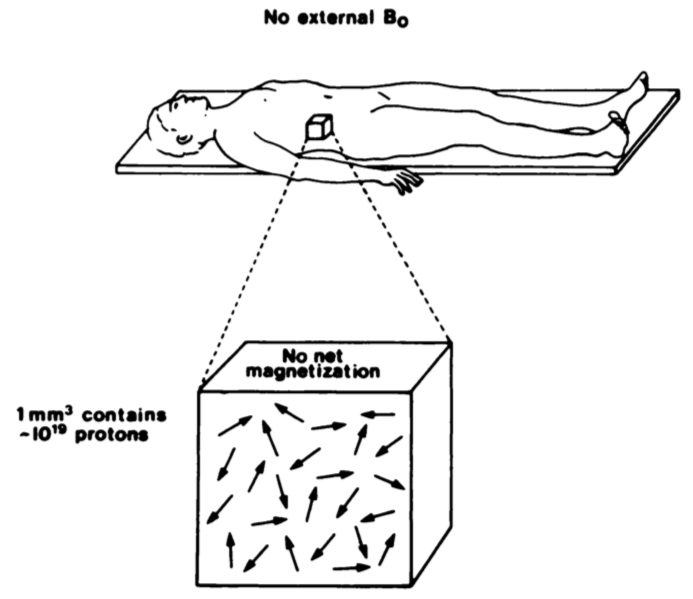
\includegraphics[scale=0.25]{media/0-imaging/mr1a.png}
\label{fig:mr11}}
\subfigure[]{%
		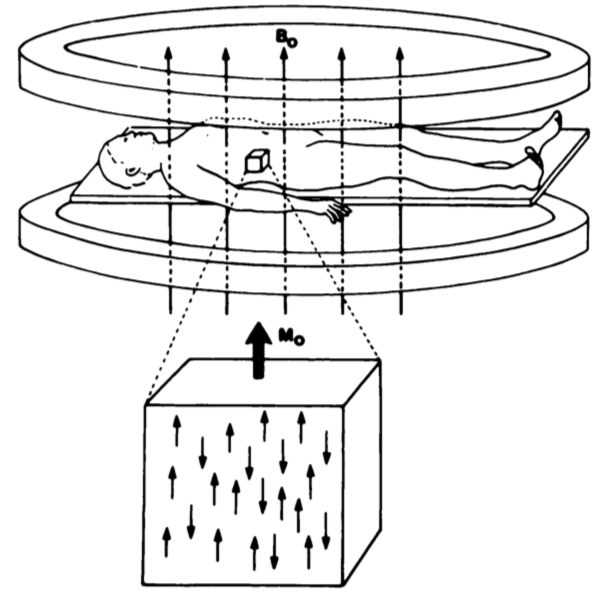
\includegraphics[scale=0.25]{media/0-imaging/mr1b.png}
\label{fig:mr12}}
%
\caption{Net magnetization $M_0$ in a voxel of tissue (a) prior to, and (b) following the application of a static external magnetic field $B_0$~\cite{hendrick_1994}}
\label{fig:mr1}
\end{figure}

If the net magnetization is perturbed from pointing in the same direction of a magnetic field $B\bm{e}_z$, the new magnetization $M$ \textit{precesses} about the $z$ axis. The \textit{precessional frequency} or \textit{Larmor frequency} $\omega$ is defined by the relationship:
\begin{equation}
\omega = \gamma B
\end{equation}
where the constant $\gamma$ is the \textit{gyromagnetic ratio}, which is 42.6 MHz/T for hydrogen. In MR imaging, the net magnetization is tipped away from the direction of $B_0$ by applying a radio-frequency (RF) pulse that oscillates exactly at the Larmor frequency. The precessing transverse magnetization produces a changing magnetic field, which induces an electric current and is recorded by the receiver coil (see \figref{mr2}).

\begin{figure}[ht]
\centering
\subfigure[]{%
		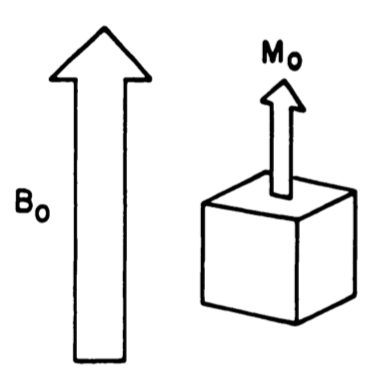
\includegraphics[scale=0.25]{media/0-imaging/mr2a.png}
\label{fig:mr21}}
\subfigure[]{%
		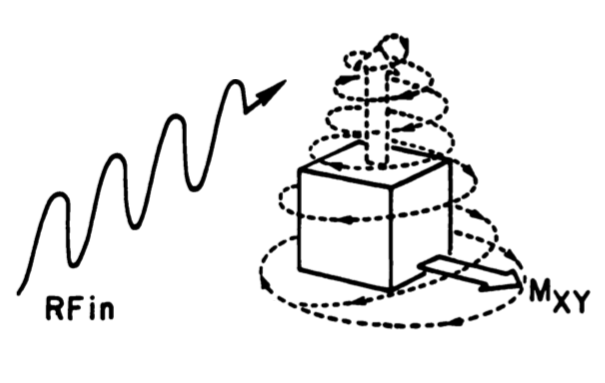
\includegraphics[scale=0.25]{media/0-imaging/mr2b.png}
\label{fig:mr22}}
\subfigure[]{%
		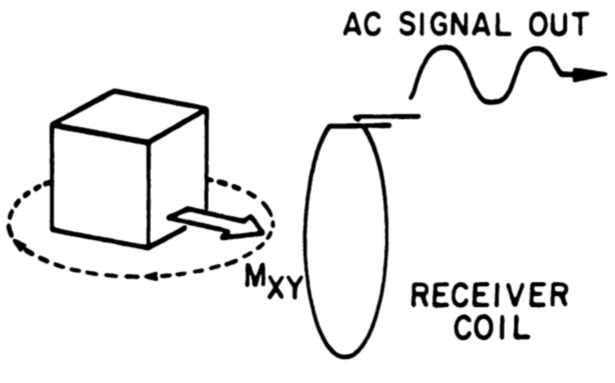
\includegraphics[scale=0.25]{media/0-imaging/mr2c.png}
\label{fig:mr23}}
%
\caption{Basic premise of MRI: (a) An external magnetic field $B_0$ causes a net magnetization $M_0$ of a voxel of tissue pointing in the same direction as the applied field, (b) an RF pulse applied at the precessional frequency of hydrogen causes the magnetization vector to tilt from a longitudinal direction into the transverse plane, and (c) the amplitude, frequency, and phase of the time-varying signal from the transverse magnetization $M_{xy}$ is recorded~\cite{hendrick_1994}}
\label{fig:mr2}
\end{figure}

In order for the receiver coil to distinguish between different locations in the object, \textit{spatial localization} of the MR signal is achieved by applying linear magnetic field gradients in each of the three spatial directions. Namely, the new spatially varying magnetic field $B(\bm{x})\bm{e}_z$ (still pointing in $z$ direction), following the imposition of magnetic gradients, becomes:
\begin{equation}
B(\bm{x}) = B_0 + \bm{G}(t) \cdot \bm{x}
\label{eqn:gradient}
\end{equation}
Multiplying \eqnref{gradient} by $\gamma$ yields:
\begin{equation}
\omega(\bm{x}) = \omega_0 + \bm{G}(t) \cdot \bm{x}
\label{eqn:freq}
\end{equation}
Thus, each RF signal oscillates at the appropriate frequency to excite and record information for each unique voxel in the image.

The magnetic field gradient $\bm{G}(t) = (G_x, G_y, G_z)$ is applied in stages.. Specifically, the magnetic gradient $G_z$ and corresponding RF pulse are first turned on to excite a particular slice (or section) of tissue. Excitation here refers to the perturbation of the net magnetization away from the $z$ direction into the transverse plane. $G_z$ is referred to as the \textit{slice-selection gradient}. The resolution of the image in the $z$ direction may be increased by reducing the bandwidth of the RF pulse or increasing the strength of the applied gradient. To resolve the selected section into voxels, gradients are applied separately in each of the two in-plane directions $x$ and $y$. The magnetic gradient $G_y$ is applied and removed following signal excitation. While turned on, the gradient causes strips of hydrogen nuclei within the slice to precess at different speeds for a brief period of time. When the gradient is turned off, different strips maintain the same precessional frequency within the same slice, but a fixed phase difference now exists among them. $G_y$ is referred to as the \textit{phase-encoding gradient}. Finally, the magnetic gradient $G_x$ alters the resonant frequency along the $x$ direction. It separates each strip into voxels, each voxel resonating at a different frequency. $G_x$ is applied at the time of signal measurement and is referred to as the  \textit{frequency-encoding gradient} or the \textit{readout gradient}. The resolution of the in-plane image may be improved by increasing the number of pulse sequence acquisitions and subsequent measurements. See \figref{mr3} for a visual representation of these steps.

\begin{figure}[ht]
\centering
\subfigure[]{%
		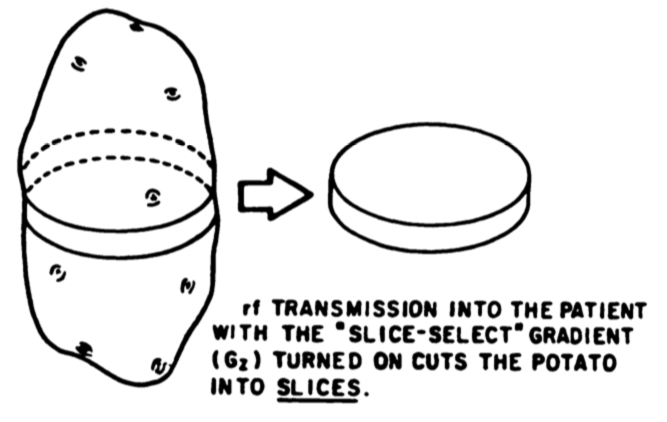
\includegraphics[scale=0.21]{media/0-imaging/mr3a.png}
\label{fig:mr31}}
\subfigure[]{%
		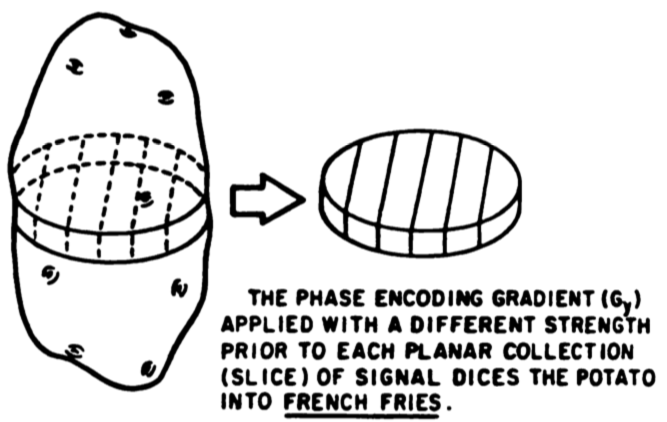
\includegraphics[scale=0.21]{media/0-imaging/mr3b.png}
\label{fig:mr32}}
\subfigure[]{%
		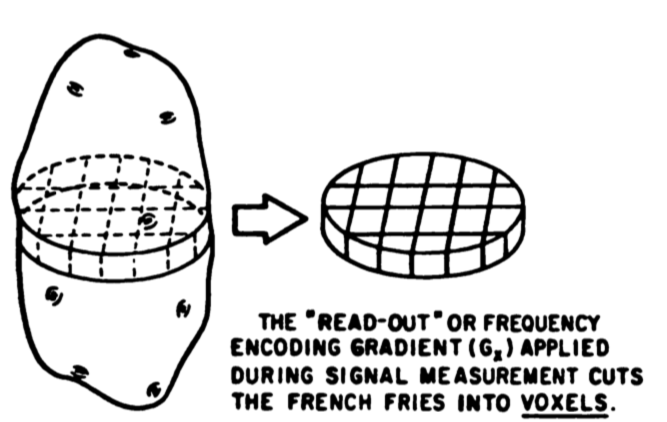
\includegraphics[scale=0.21]{media/0-imaging/mr3c.png}
\label{fig:mr33}}
%
\caption{Visual representation spatial localization based on successive application of magnetic gradients: (a) slice-selection gradient, (b) phase-encoding gradient, and (c) frequency-encoding gradient~\cite{hendrick_1994}}
\label{fig:mr3}
\end{figure}

MRI signal intensity at a particular voxel typically depends on the proton density of the tissue (via the strength of the net magnetization $M_0$) and two \textit{relaxation times} T1 and T2 corresponding to the exponential decay of the perturbed net magnetization back to its original state following an RF pulse. Following a typical $90^{\circ}$ RF pulse, which maximizes the transverse magnetization $M_{xy}$, the relaxation times are defined by the following relationships:
\begin{align}
M(t) &= M_0(1 - e^{(-t/T1)}) \\
M_{xy}(t) &= M_{xy}e^{(-t/T2)}
\end{align}
The \textit{T1 recovery time} (also known as the \textit{spin-lattice} or \textit{longitudinal recovery time}) corresponds to the recovery of the longitudinal magnetization $M_0$. This reorientation is caused by the transfer of energy from the excited magnetic dipoles to the surrounding lattice of molecules. The \textit{T2 recovery time}  (also known as the \textit{transverse} or \textit{spin-spin recovery time}) corresponds to neighboring precessing magnetic dipoles \textit{dephasing}. Dephasing occurs because as the transverse magnetization decays, slightly different magnetic environments exist for neighboring hydrogen nuclei in different regions of a particular voxel.

Tissue contrasts are created based on the strength and timing of the RF pulse; this is known as the \textit{MR sequence}. The parameters in MR pulse sequences weight the influence of proton density, T1, and T2 differently in the final MR signal. The most basic MR sequences are \textit{proton density} (PD), \textit{T1-weighted} (T1W), and \textit{T2-weighted} (T2W), each of which provide different tissue contrasts. The choice of an MR sequence will depend on the tissues and applications of interest of the scan. A number of references are available for a more detailed description of T1, T2, the parameters of an MR sequence, and their relationship in creating tissue contrast~\cite{nishimura_2010, brown_semelka_2003, webb_2003} .

For each voxel in a slice, the amplitude, phase, and frequency of the time-varying MR signal is recorded by the receiver coil in the \textit{frequency domain}, or what is known as \textit{k-space}. For each slice, the frequency domain is converted to the spatial domain (i.e., the two-dimensional image for a particular slice) via 2D inverse Fourier transform. The k-space of an image can be modified to identify artifacts, remove noise, and enhance contrast. Please refer to the references in this section for more detail on k-space and its manipulations. Finally, each 2D image is combined to form a 3D grayscale image corresponding to the object scanned. The intensity at each voxel in the three-dimensional rectilinear grid is a weighted proton density. The value at each voxel can represent many different units of measure depending on the pulse sequence~\cite{beek_hoffman_2008}.

\subsection{X-Ray Computed Tomography}
\label{X-Ray Computed Tomography}

X-ray computed tomography (CT) is the process of generating images via the emission of an x-ray beam source, and subsequently detecting the \textit{attenuation} of the x-ray beam through the various tissues in the patient or object. CT provides excellent contrast for bone, but is less suitable in measuring soft tissue contrast compared to MRI. Acquisition times are typically less than those for MRI, image resolutions are typically higher~\cite{pomeranz_2007}, and ionizing radiation from the x-ray beam must also be carefully considered. The basic principles of image acquisition via CT technology ensue.

In CT, an x-ray beam source is emitted through the plane of a finite thickness cross section of the object~\cite{mahesh_2002}. The mean attenuation of the x-ray beam through each voxel within the slice is measured by a detector on the other side of the object. The attenuation data is reconstructed into a digital two-dimensional image. Once again, the set of 2D images is stacked together to form a 3D image representation of the region being scanned.

Attenuation measures the amount by which x-ray radiation is reduced in passing through a material. For an inhomogeneous material, the attenuation along a particular ray line is expressed in the following relationship:
\begin{equation}
I= I_0e^{-\int\limits_{0}^{L}f(x,y) ds}
\label{eqn:init}
\end{equation}
where $I_0$ is the x-ray intensity emitted in front of the object, $I$ is the x-ray intensity received behind the object, $f(x,y)$ is the linear attenuation coefficient for the material at location $(x,y)$, $L$ is the length over which the beam travels through the material, and $ds$ is the length of a differential cut along the ray. The variable $s$ is parameterized as a function of $x$ and $y$. In first generation CT machines, for a particular slice, the x-ray tube and detector were rigidly translated together across the subject as x-ray beams were emitted and recorded~(see \figref{ct1}).

\begin{figure}[ht]
\centering
		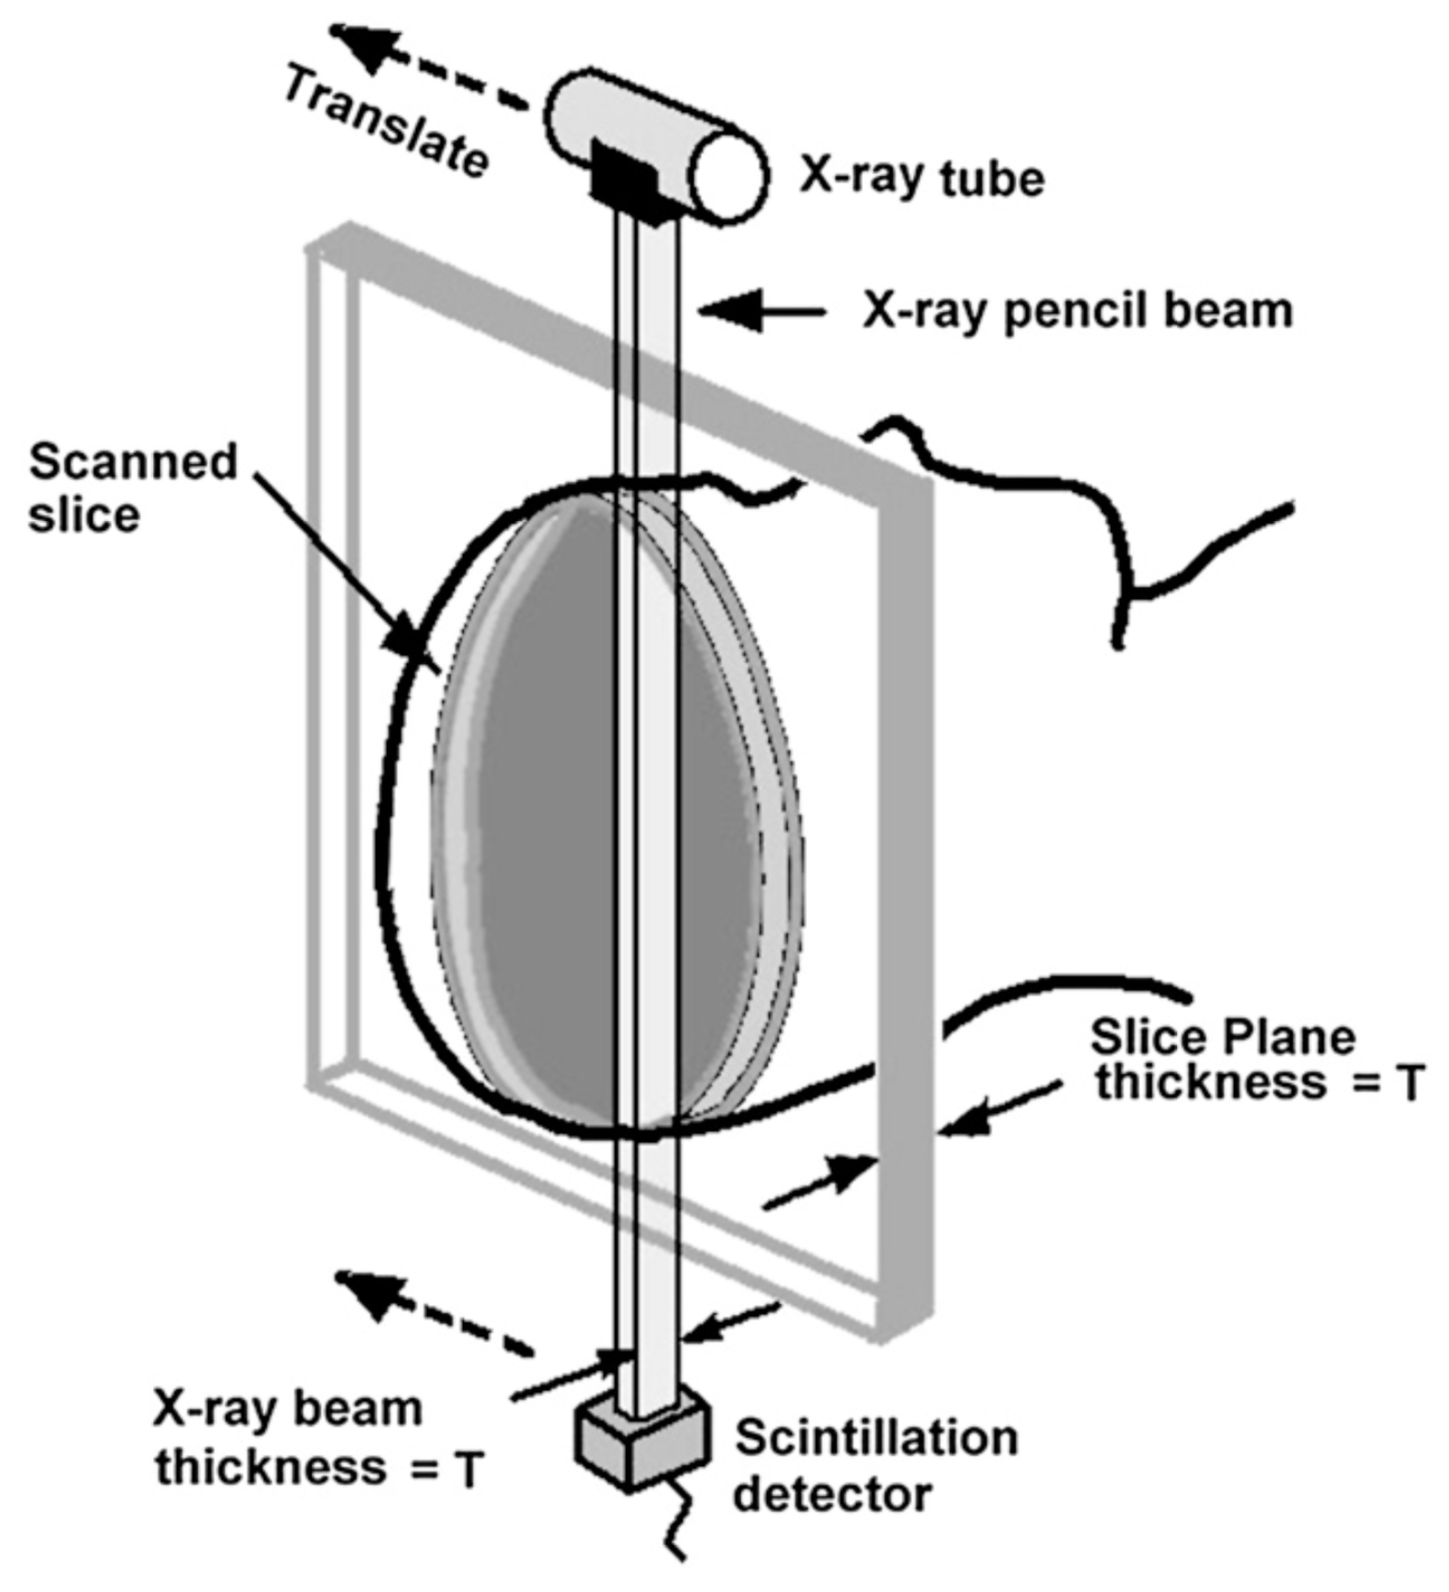
\includegraphics[scale=0.3]{media/0-imaging/ct1.png}
%
\caption{CT arrangement for linear transverse scanning motion of x-ray tube and detector. ~\cite{goldman_2007}}
\label{fig:ct1}
\end{figure}

The x-ray beam path is referred to as a \textit{ray}. The set of rays and measurements made during the translation is known as a \textit{view}. Several hundred rays are measured in a particular view. The assembly is then rotated about the axis perpendicular to the slice plane by a small increment and a new view is captured. Over 1000 views are captured as the assembly is rotated through 360$^{\circ}$. Thus, the total number of measurements for a particular slice is the number of rays per view multiplied by the number of views, and is on the order of one million measurements per slice in modern CT machines (see \figref{ct2}).

\begin{figure}[ht]
\centering
		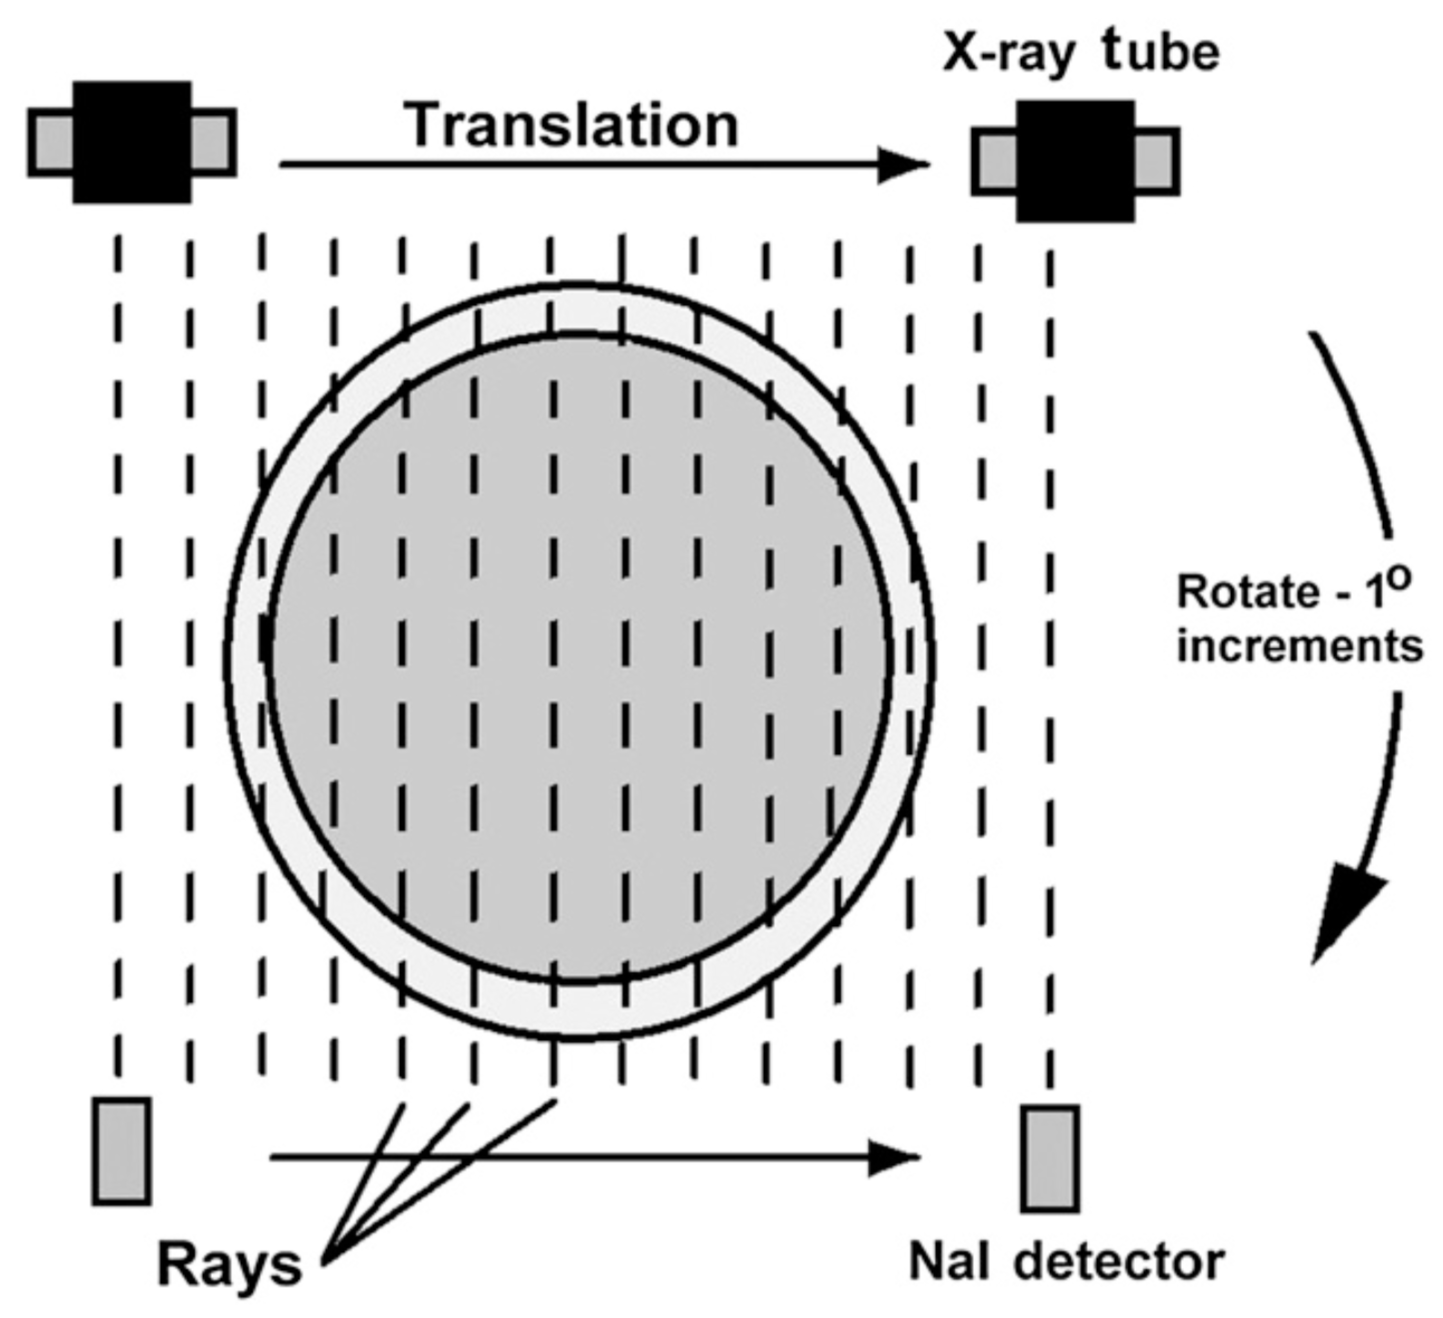
\includegraphics[scale=0.3]{media/0-imaging/ct2.png}
%
\caption{Measurement procedure for first-generation CT. Rays are emitted from the x-ray tube and the attenuated radiation is measured by the detector. The assembly is translated in increments to cover the span of the slice. The process is repeated as the assembly is rotated in increments through 360$^{\circ}$~\cite{goldman_2007}}
\label{fig:ct2}
\end{figure}

\textit{Image reconstruction} is the process of deriving the average attenuation coefficient values $f$ for each voxel in a slice from the attenuation measurements made by the x-ray detector. Attenuation increases with the density and atomic number of the tissues in the voxel. Rearranging~\eqnref{init} yields:
\begin{equation}
p(\xi, \theta) = -\ln(I/I_0) = \int\limits_{0}^{L}f(x,y) ds
\end{equation}
The function $p(\xi,\theta)$ is known as the \textit{Radon transform} of the attenuation function $f(x,y)$. The angle $\theta$ corresponds to the angle of rotation of the view, and $\xi$ corresponds to the position along the measured x-ray projection~(see \figref{ct3}).

\begin{figure}[ht]
\centering
		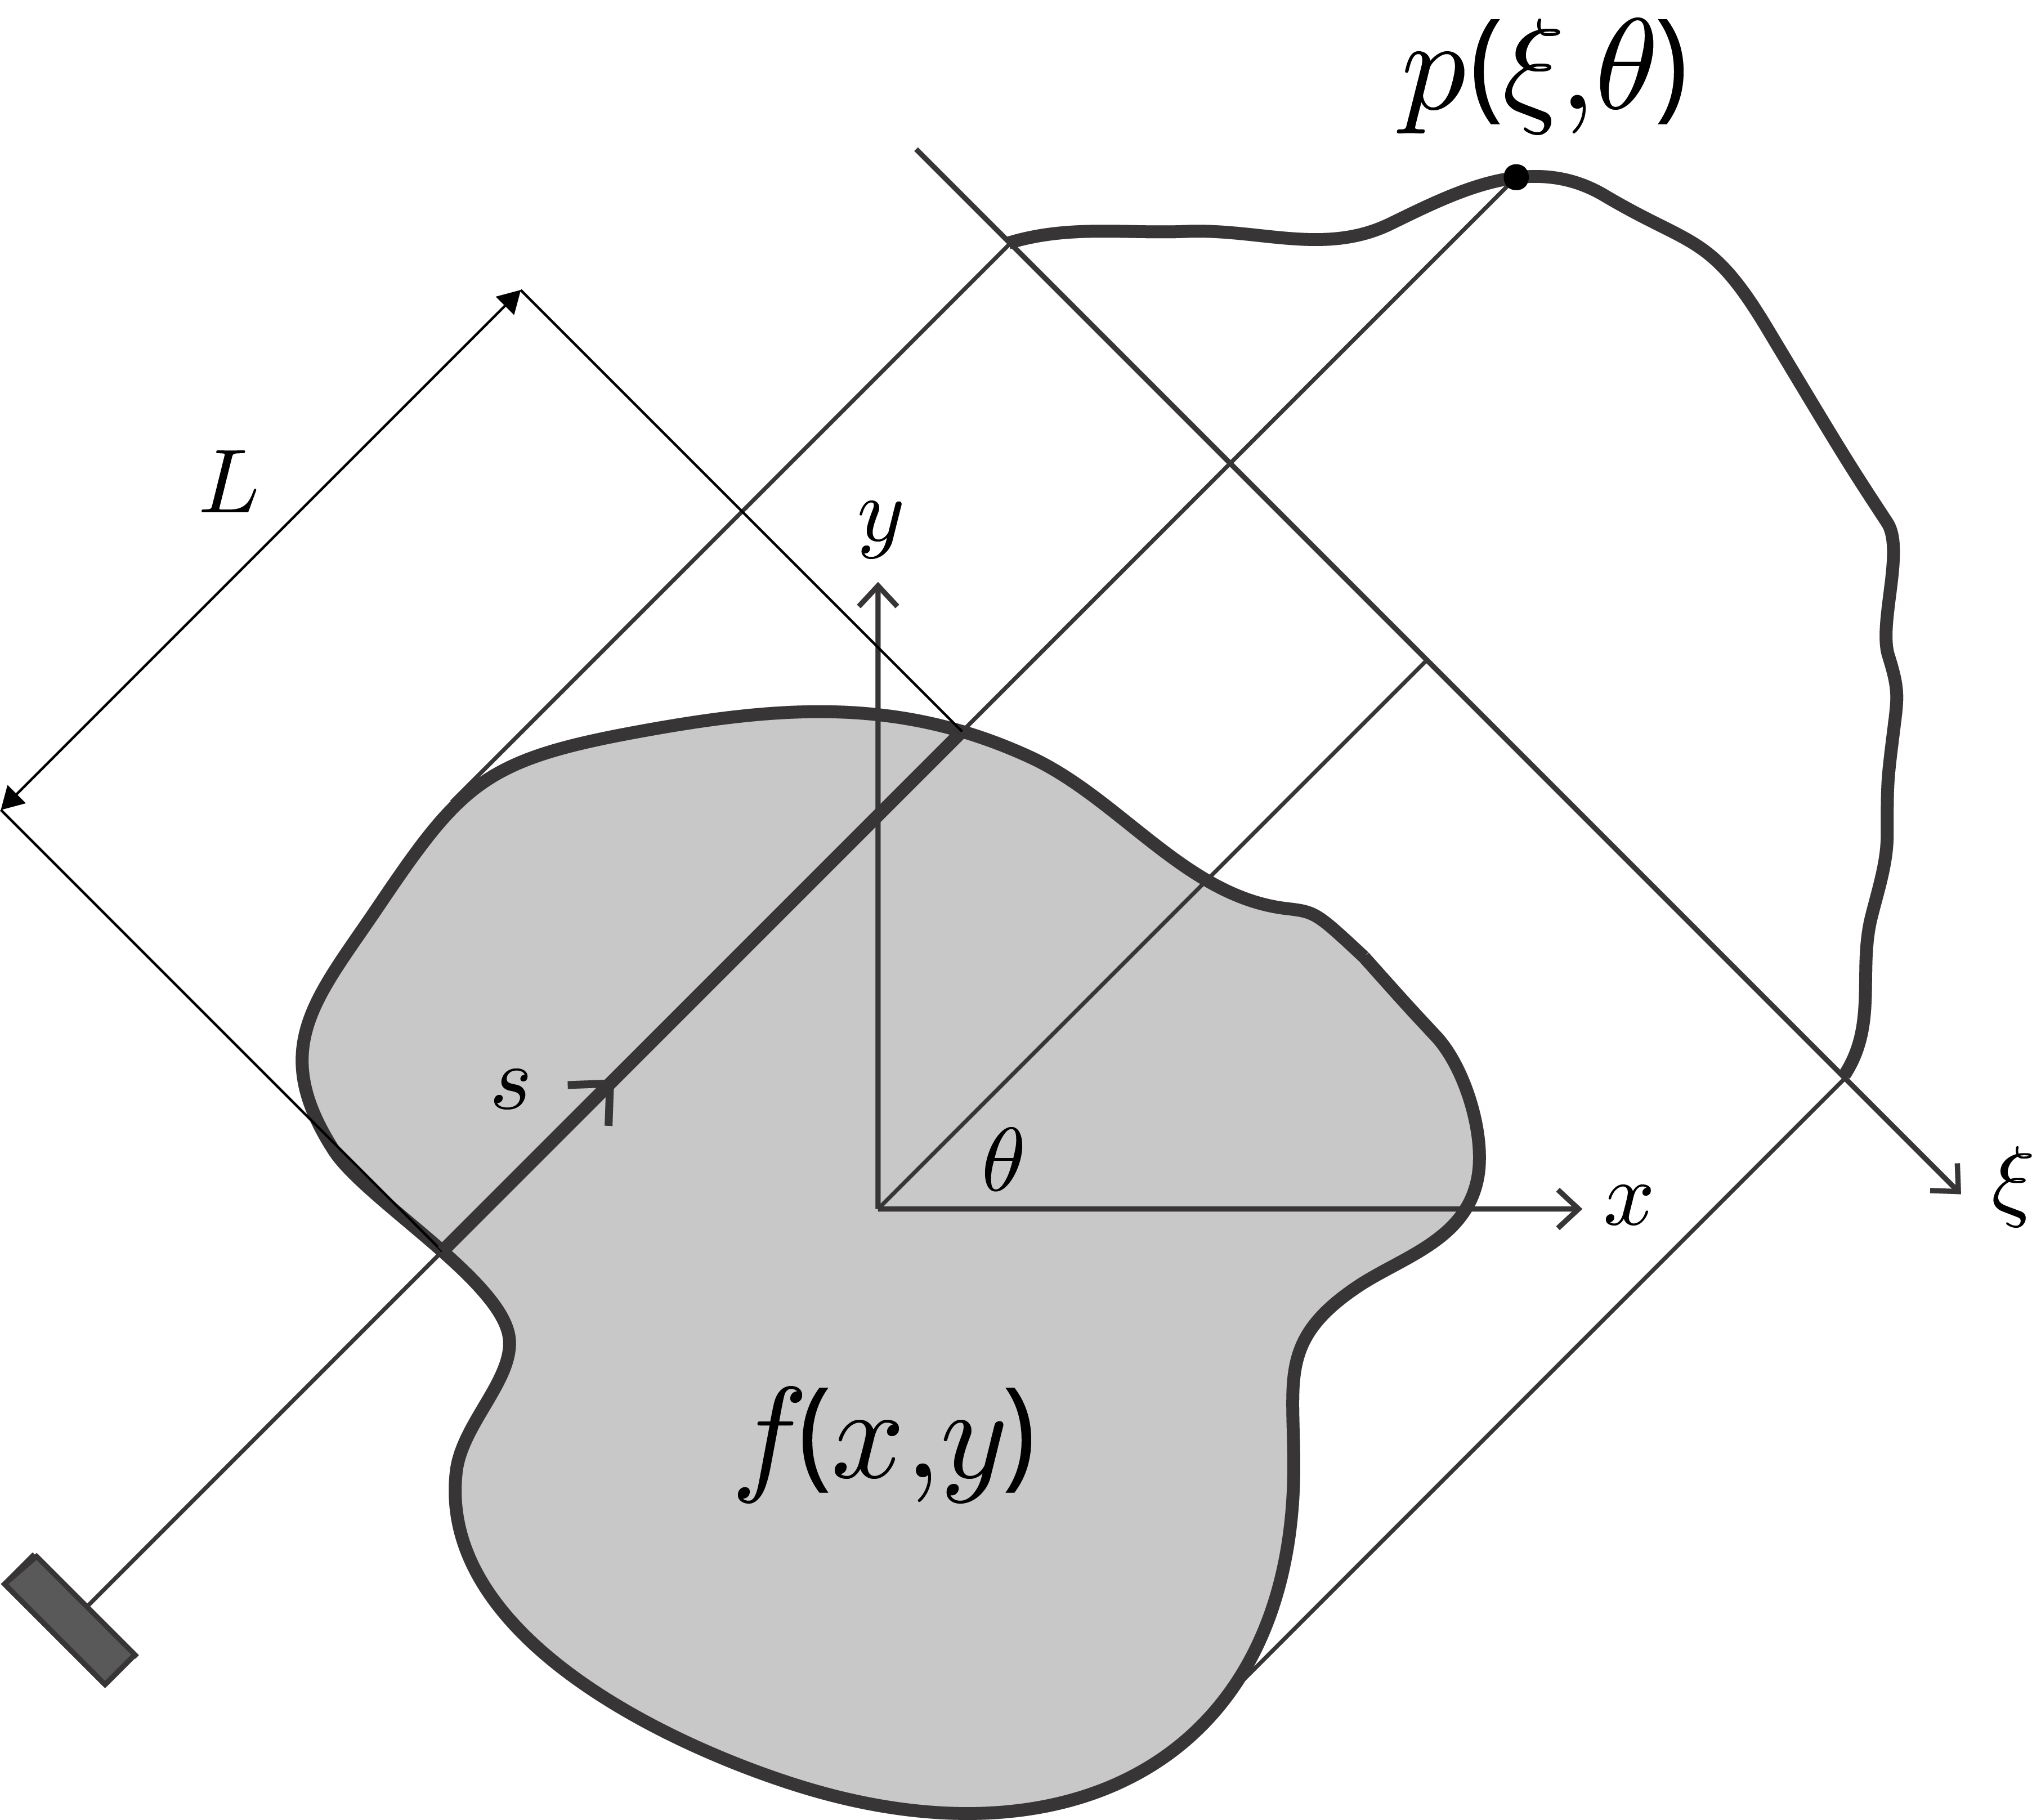
\includegraphics[scale=0.3]{media/0-imaging/ct3.png}
%
\caption{Linear attenuation function $f(x,y)$ for a particular slice, and corresponding projection $p(\xi,\theta)$}
\label{fig:ct3}
\end{figure}

The function $p$ for each $\theta$ view is known as a \textit{projection} of the image $f$. The most popular image reconstruction technique is \textit{backprojection}, in which the function $f$ is computed from the projections $p$. Backprojection leads to a blurring of the original image, so the projected images are first filtered prior to backprojection. The total technique is known as \textit{filtered backprojection}. The Fourier transform of $p$ is computed, a ramp filter is applied in frequency space, the inverse Fourier transform of the resulting function is computed, and finally the inverse Radon transform is applied to approximate $f(x,y)$. Filtered backprojection performs best in the presence of a large number of projections, which is the case in modern CT scanners. A more detailed description of the procedure is provided by Chetih \textit{et al.}~\cite{chetih_2015}.

Finally, the value computed at each voxel is rescaled to produce the \textit{CT number}. The CT number is defined as $K (f_i - f_w)/f_w$, measured in \textit{Hounsfield units}. The scaling parameter $K$ is typically a value of 1000 in modern machines. The value $f_i$ is the attenuation at a particular voxel, and the value $f_w$ is the attenuation of water. The attenuation coefficient of water is obtained during calibration of the machine.

Improvements in acquisition times, spatial resolution, and image reconstruction times have been made in the last 45 years since the first-generation CT machine was introduced. These improvements mostly involve an increase in x-ray detectors and more clever arrangements and motions of the x-ray beam and associated detector(s). Detailed descriptions of these improvements can be found in the references cited in this section.

\subsection{Additional Imaging Modalities}
\label{Other Imaging Modalities}

Several other popular imaging modalities exist in addition to MRI and CT. The discussion here will be restricted to a brief overview of \textit{ultrasound} (US), as well as some quantitative variations of MRI, CT, and US.

Ultrasound uses high-frequency sound pulses that are emitted from a hand-held ultrasound transducer~\cite{waldman_campbell}. The transducer is applied to the patient's skin through a coupling gel, and sound pulses are reflected back to the transducer from structures within the patient. The magnitude of the reflected sound, or \textit{echo}, is converted into a 2D grayscale image. Images are acquired in real-time, and do not require any ionizing radiation. Ultrasound is most commonly used for imaging the abdominal and pelvic regions, as well as imaging the musculoskeletal system. When used to image the heart, ultrasound is referred to as \textit{echocardiography}. Three-dimensional ultrasound techniques have been gaining traction in recent decades, of which there are two varieties for 3D reconstruction: random or \textit{freehand scanning} which is based on free motion of the ultrasound transducer; and \textit{sequential scanning} where the ultrasound motion is predetermined in linear, fan-like or rotational patterns~\cite{valocik_2005, bruining_2000}.

Quantitative versions of the modalities discussed attempt to extract material property information in addition to only contrasting different tissues. \textit{Diffusion-tensor imaging} (DTMRI) is used to measure the anisotropy of tissues. Additional magnetic field gradients are applied repeatedly to create images that are sensitized to the diffusion of water in specific directions~\cite{o'donnell_westin_2011}. The diffusivity tensor is approximated at each voxel, and may be used to visualize irregularities in the microstructure of the brain~\cite{alexander_lee_lazar_field_2007}, or to approximate cardiac muscle fiber orientations. \textit{Elastography} is the process of quantitatively imaging the mechanical properties of soft tissues \textit{in vivo}, and is performed using either magnetic resonance or ultrasound techniques~\cite{zaleska_2014}. The process involves first applying a stress or source of motion that deforms the tissue, next imaging the tissue response, and finally processing the data to generate images (\textit{elastograms}) of tissue mechanical properties~\cite{glaser_manduca_ehman_2012}. \textit{Quantitative computed tomography} (QCT) estimates bone mineral density from CT attenuation data by using a calibration phantom during image acquisition. This information can be used to inform heterogeneous material definitions in computational models of bone~\cite{knowles_2016}.

A more complete review of medical imaging technologies can be found in a number of texts~\cite{webb_2003, suetens_2017}.

\subsection{File Formats}
\label{Data Format-IMG}

Medical images are typically stored as a combination of a short \textit{header} followed by \textit{voxel data}. The header is typically stored in ASCII format and the voxel data is typically binary. They may be found in the same file or in separate ones. Voxel data is often stored either as a set of two-dimensional images representing each slice, or as a single block of information corresponding to the 3D volume. In either case, data is stored as a 1D array, from which the data can be unrolled based on the axis ordering specified in the header. The header provides metadata to allow software to read and store the image based on the voxel data. Namely, the header contains the matrix dimensions, image resolution, image origin, axis order, data type of the voxel data (i.e., unsigned char, int, etc.), endianness of the voxel data, and data compression encoding (e.g., raw, gzip, bzip2). Additional information may be provided as well, including patient data, image acquisition parameters (e.g., MRI pulse sequence), and date of acquisition. On the clinical side, DICOM (Digital Imaging and Communications in Medicine) files are by far the most popular format for storing medical images, due to it's extensive metadata including patient information and image acquisition protocol. Several formats are available in research, including MATLAB, NRRD (Nearly Raw Raster Data), NIfTI (Neuroimaging Informatics Technology Initiative), and Analyze. These file formats are different flavors of the same general format described above. By containing less detailed and cumbersome metadata sections, they are geared more towards image post-processing compared to DICOM.

%%%%%%%%%%%%%%%%%%%%%%%%%%%%%%%%%%%%%%%%%%%%%%%
%%%%%%%%%%%%%%%%%%%%%%%%%%%%%%%%%%%%%%%%%%%%%%%
\section{Image Segmentation Approaches}
\label{Image Segmentation Approaches}

Arguably the most challenging step in producing a robust workflow is the subsequent processing and segmenting of the image of interest. \textit{Image segmentation} is the process of partitioning an image into nonoverlapping regions corresponding to different tissues or objects in an image. Contrast differences between neighboring tissues can be difficult to identify, and thus \textit{image processing} is first performed.

\subsection{Image Processing}
\label{Image Processing}
In image processing, filters are applied to the image to alter voxel intensity values, which can remove noise and emphasize features of the image so as to improve the performance of image segmentation algorithms. Processing the image data begins with \textit{resampling}. Images almost always have a higher resolution in-plane than in the slice direction. Segmentation techniques typically prefer \textit{isotropic voxel spacing}, meaning the resolution of the image is the same in all three directions. Thus, images are resampled such that isotropic voxel spacing is achieved. Resampling simply involves interpolating voxel data from the original coarser image to the new voxel locations of the artificially finer resampled image. Any number of interpolation bases may be used, but practically speaking the basis choice is insignificant for images with clinical resolutions, and can be as simple as linear interpolation.

The image is additionally processed to remove noise and artifacts, as well as to emphasize tissue interfaces for more successful application of image segmentation techniques. Image filters include the \textit{Gaussian blur filter}, \textit{mean filter}, and \textit{median filter}~\cite{Seg3D}. Each of these are known as smoothing filters, but in fact facilitate the identification of tissue interfaces by producing larger regions of more homogeneous voxel intensities. The median filter is particularly effective in reducing the \textit{salt and pepper sign} commonly found in MRI, in which tissues have a speckled appearance.

\subsection{Review of Image Segmentation Approaches}
\label{Review of Image Segmentation Approaches}

Following resampling and processing, image segmentation is performed to identify the tissues and objects of interest. If the domain of the image is given by $\Omega$, the segmentation problem is to determine the sets $S_k \subset \Omega$, such that:
\begin{align}
\Omega &= \bigcup \limits_{k=1}^{K} S_k \\
S_k \cap S_j &= \emptyset, \text{\ \ } k \neq j
\end{align}
where $K$ is the total number of classifications in the image. Often, the value of K is assumed to be known based on prior knowledge of the anatomy being considered~\cite{pham_2000}. Each voxel in the image is assigned a tag corresponding to the region to which it belongs, resulting in what is known as an \textit{image mask}, as shown in~\figref{seg}. An enormous number of image segmentation techniques exist in the literature; a few popular techniques are mentioned here.

\begin{figure}[ht]
\centering
\subfigure[]{%
		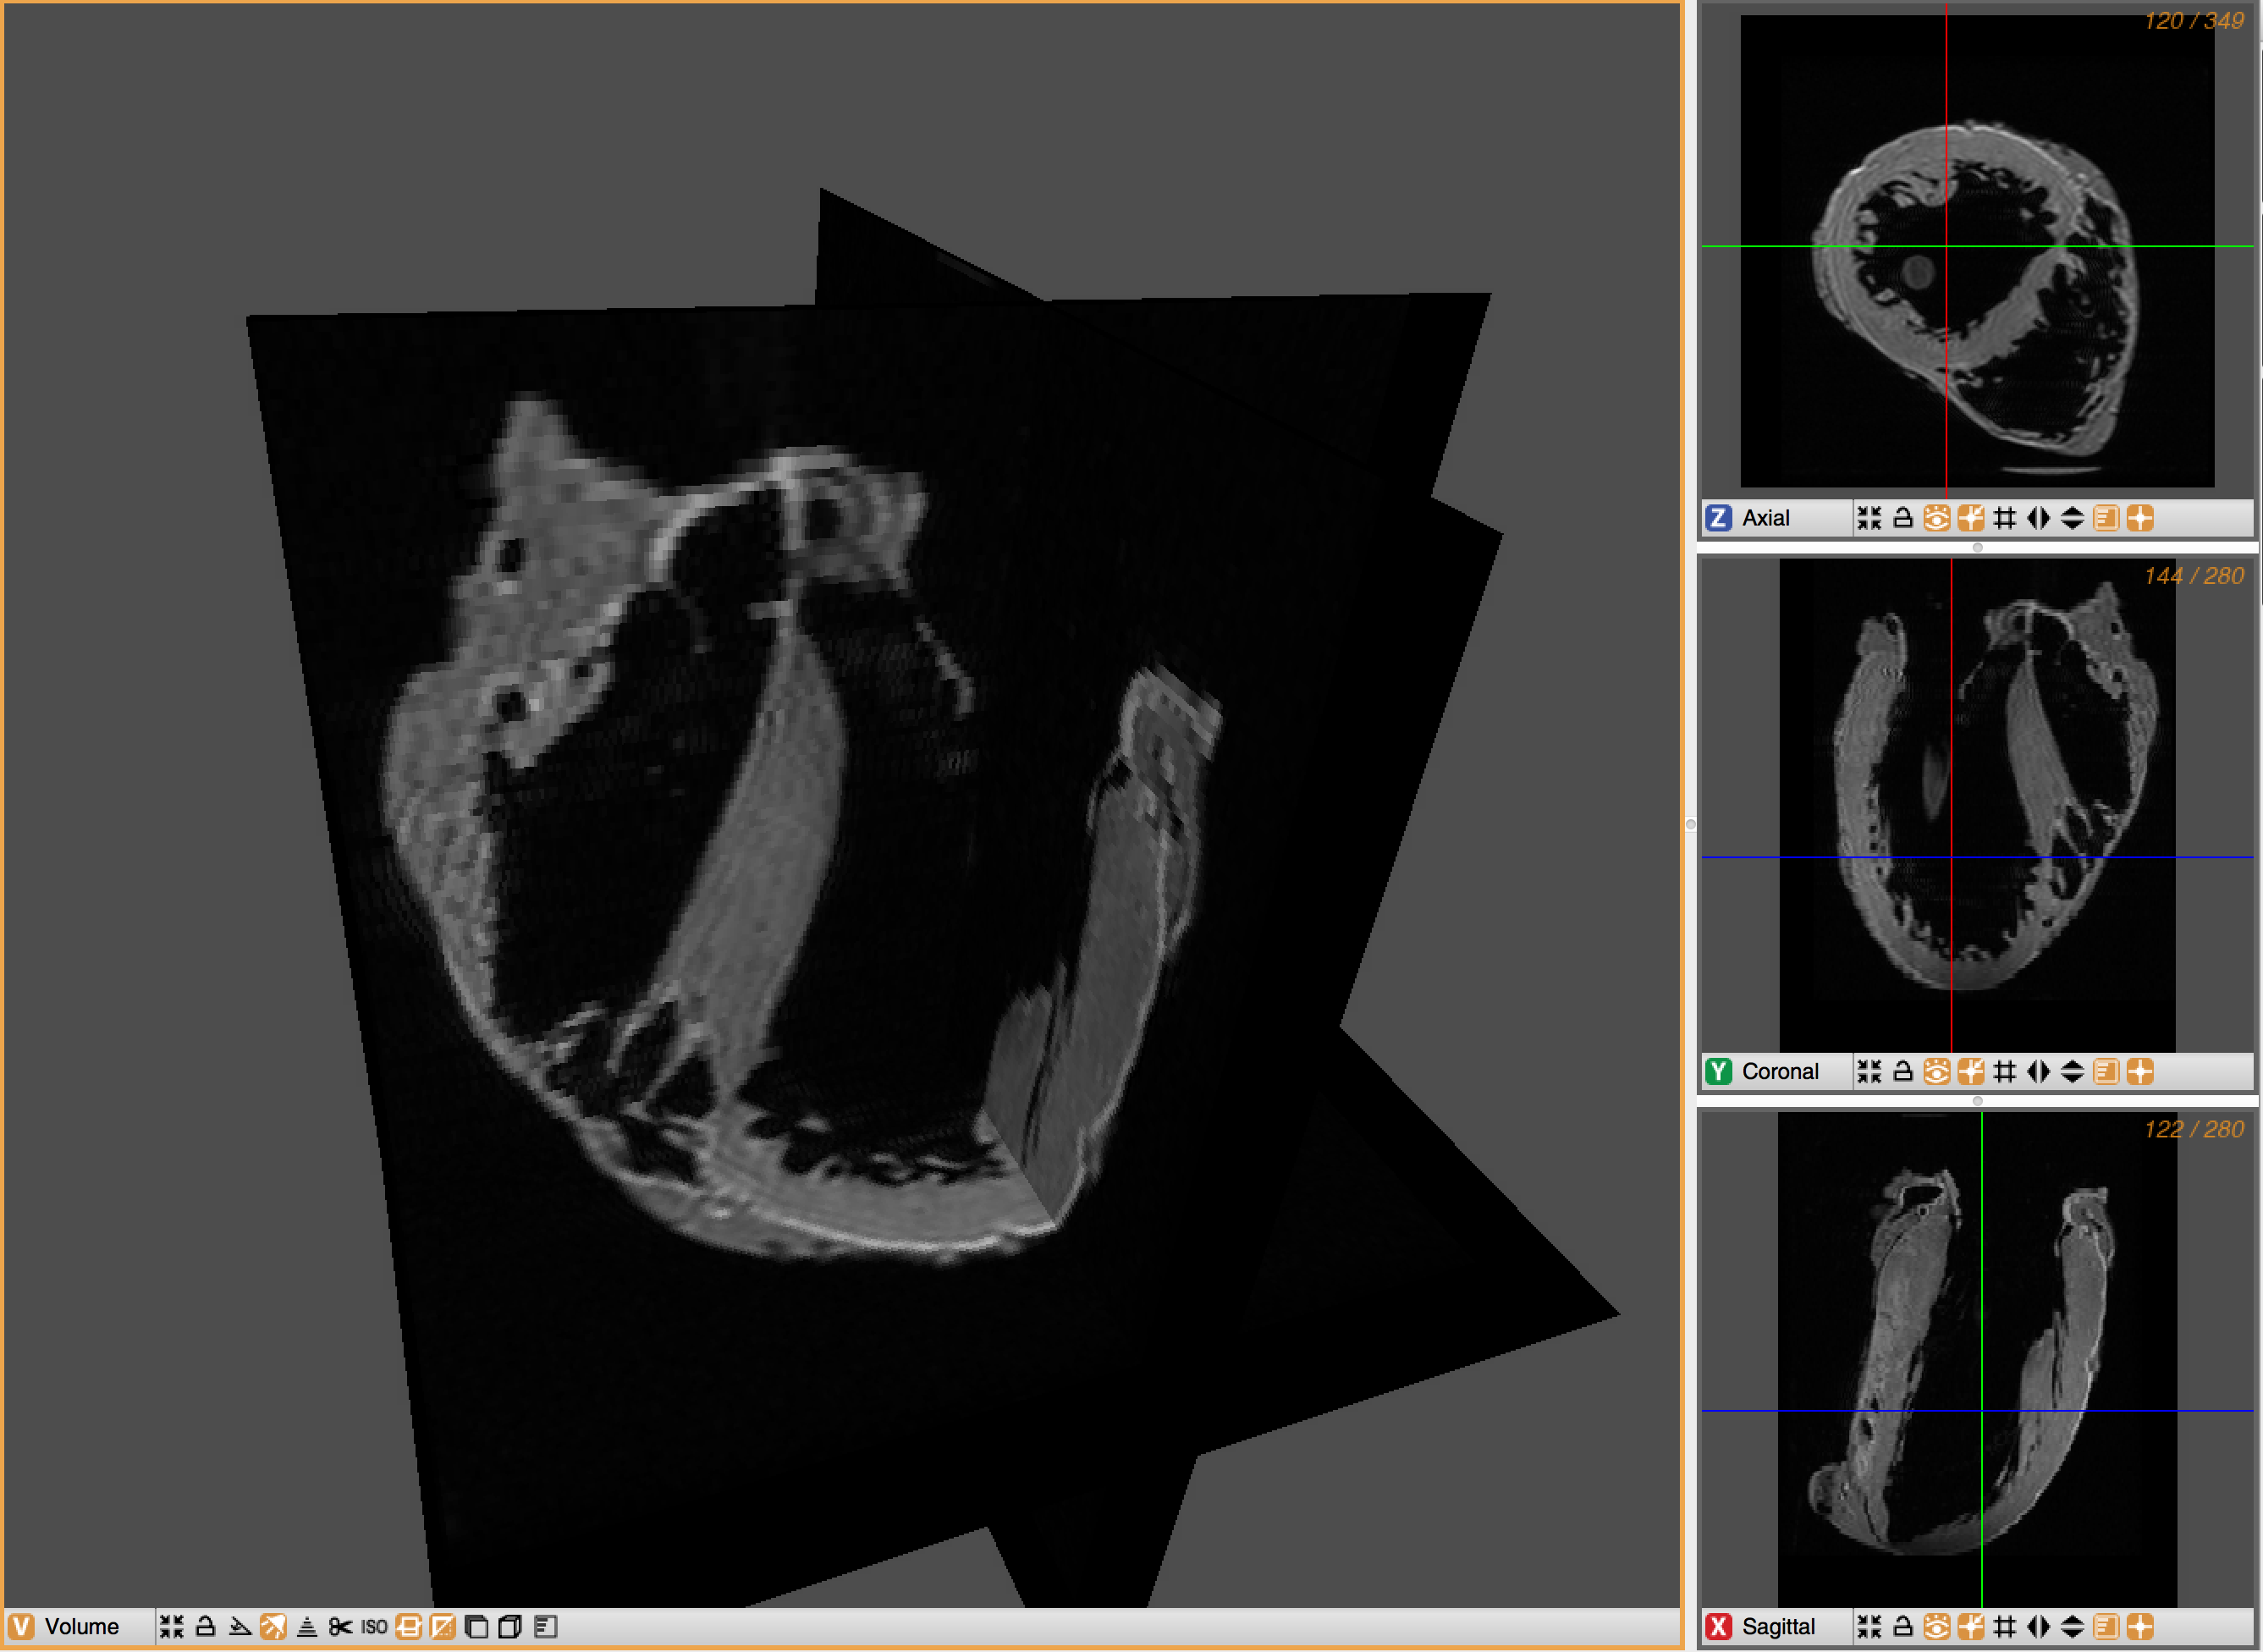
\includegraphics[scale=0.165]{media/1-seg3d/1-raw.png}
\label{fig:seg1}}
\subfigure[]{%
		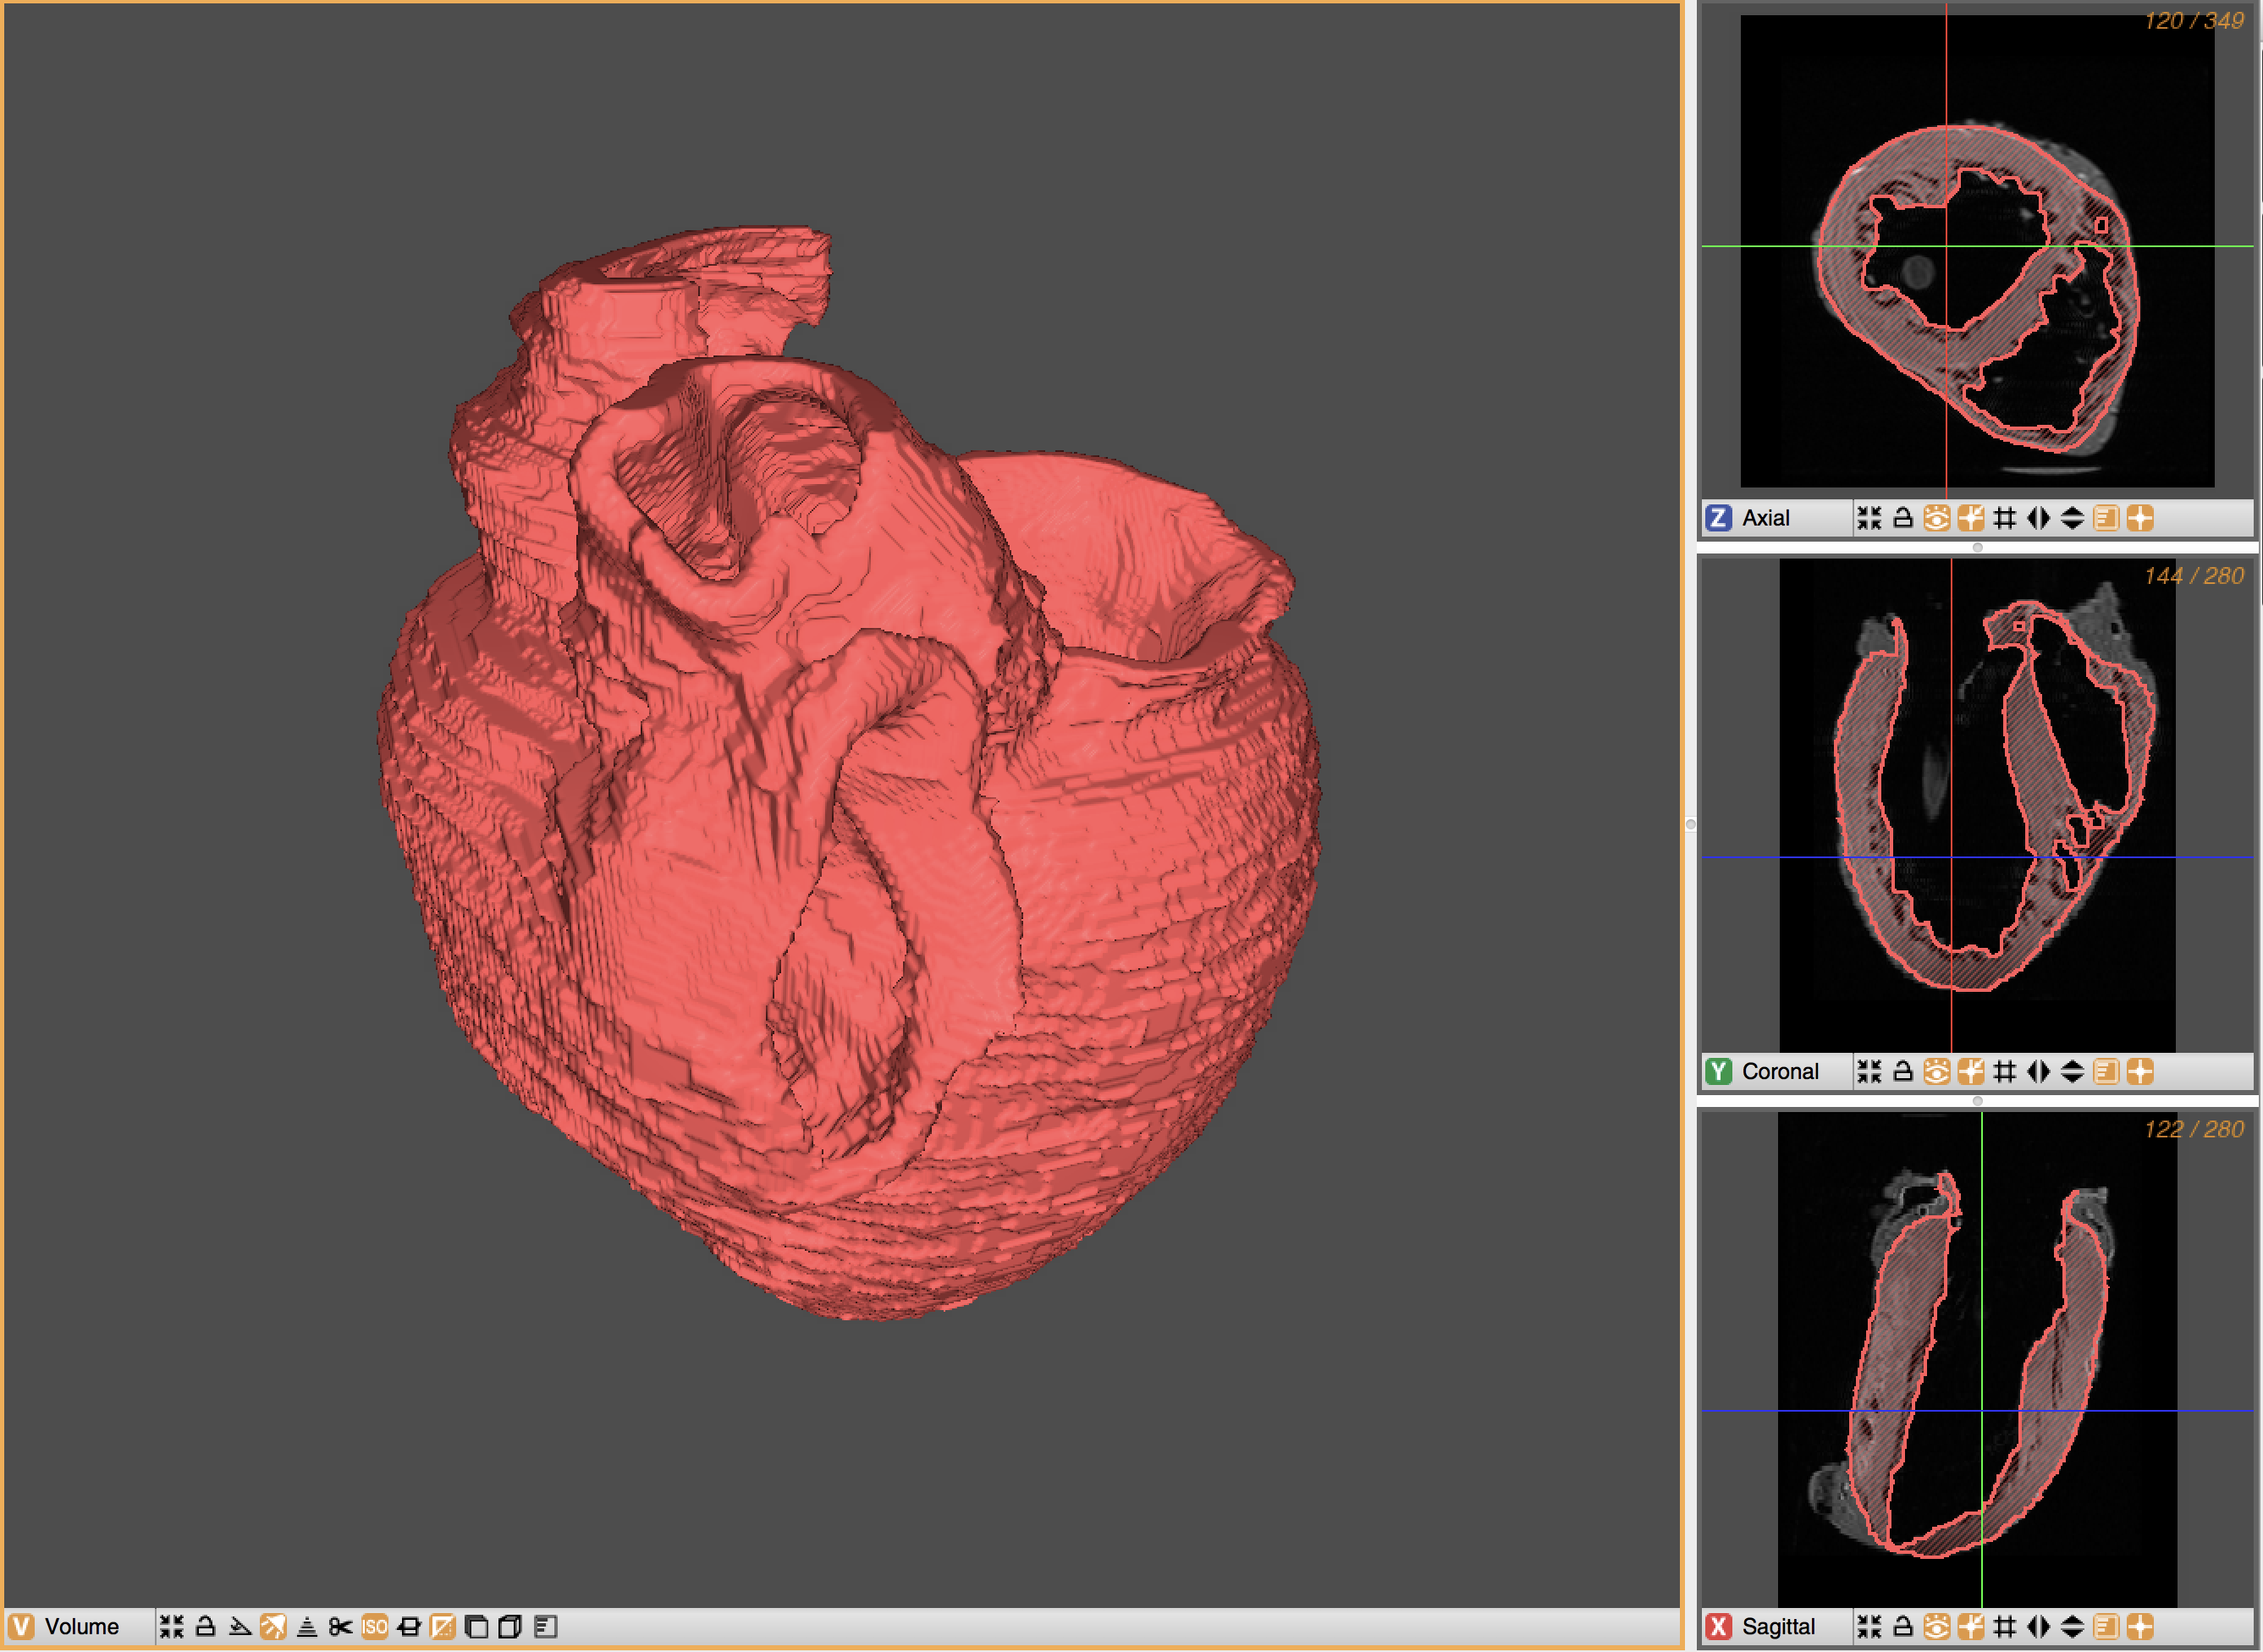
\includegraphics[scale=0.165]{media/1-seg3d/2-seg.png}
\label{fig:seg2}}
%
\caption{(a) MRI of \textit{ex-vivo} human heart, and (b) resulting segmented image mask}
\label{fig:seg}
\end{figure}

\textit{Thresholding} delineates images based on voxel intensities alone. A thresholding procedure attempts to determine the intensity value - the threshold - that separates two different regions. A histogram of image intensities may have several modes depending on the number of regions $K$, though, so several thresholds are generally applied (known as \textit{multithresholding}). These threshold values are selected based on the local minima present in the intensity histogram. Thresholding is often performed interactively, based on the operator's visual assessment of the resulting segmentation. It does not take into account the spatial characteristics of an image, which causes it to be sensitive to noise and intensity inhomogeneities. \textit{Region-based segmentation} merges or splits regions of voxels based on whether they share homogeneity criteria. \textit{Edge detection techniques} determine the edges of distinct regions based on gradients of the image intensity. Edge detection is not on its own a segmentation technique, but rather must be used in conjunction with region-based approaches to generate a segmentation. For example, following edge detection, a seed of voxels may be grown until the edges are reached.

\textit{Deformable models} use parametric surfaces that deform under the influence of artificial internal and external forces relating to characteristics of the image. A seed surface is initiated by the user, followed by an iterative process in which the surface deforms to the shape of the interface in the image. Internal forces aim to keep the surface smooth during deformation, and external forces drive the surface toward the desired shape. A particularly well known and effective set of approaches are \textit{level set methods}. In these approaches, a level set surface $\phi$ begins as a signed distance function $d(\bm{x})$ from the seed surface and evolves toward the desired surface with a speed whose normal component is $F$. The \textit{level set equation} is an advection equation that has the following form:
\begin{align}
\frac{\partial \phi}{\partial t} + F \left| \nabla \phi \right| = 0 \\
\phi(t=0) = d(\bm{x})
\end{align}
The front speed $F(\bm{x})$ depends on the gradient of image intensity and the curvature of the surface. This advection equation is solved using ordered upwind methods, most notably the \textit{fast marching method}~\cite{malladi_1995, sethian_1996}. The converged solution is the resultant surface for which $d = 0$. Being an implicit function, it must still be converted to an explicitly defined image mask, in the same way that edge detection methods rely on region-based methods.

\textit{Atlas guided approaches} treat segmentation as a \textit{registration} problem in which a presegmented atlas (or template) image is transformed to a target image requiring segmentation. Atlas-guided approaches are best suited for segmentation of structures that are stable over the population of the study, and may require manual selection of landmarks to constrain the nonlinear registration process. \textit{Machine learning methods} make use of \textit{neural networks} in which a set of weights associated with the nodes in a learning network are adapted based on \textit{training data}. See Litjens \textit{et al.} for a detailed description~\cite{litjens_2017}.

Many other image segmentation techniques exist, including \textit{classifier methods} and \textit{clustering methods}. The literature referenced in this section provide a detailed description of these other techniques.

Practically speaking, image segmentation algorithms to date are not typically robust enough for automated general purpose applications. In almost all cases, manual interaction and/or post-processing are required or at least preferable. Human intervention can unfortunately be laborious and time-consuming, though, and raises reliability issues for large population studies. Additionally, segmentations are typically most effective when multiple algorithms are used in conjunction with one another. For example, an image mask generated by thresholding is a an effective initial seed to region-based and deformable model approaches. Commercial and free software with graphical user interfaces (GUIs) significantly facilitate using multiple segmentation techniques, not the least of which manual fine-tuning techniques such as \textit{paintbrush} tools. Of the most popular tools available are OsiriX, Simpleware, Mimics, and Seg3D. Producing accurate image masks in a timely manner is to date still as much an art as it is a science.

\subsection{File Formats}
\label{Data Format-SEG}

Image masks are typically stored in the same format as the image data themselves, as described previously. The data at each entry in the matrix is simply an unsigned integer corresponding to the region to which the voxel belongs. The background, also referred to as \textit{void}, is assigned a value of 0. Image masks of a single tissue or object are known as \textit{binary masks}, for which voxel entries only have values of 0 for void or 1 for the tissue of interest.

%\chapter{Image-Based Meshing}
\label{chap:3}

\textit{Image-based meshing} is the process of generating explicitly defined volume meshes from imaging data for the purposes of 3D printing, visualization, or physics-based simulation. This discussion will focus on generating meshes specifically from segmented image data. The term \textit{explicit} refers to defining the mesh in terms of vertex coordinates, corresponding polytopes, and the connectivity of those polytopes, as opposed to an \textit{implicit} definition in which the surface is defined as the zero-set of a 4D \textit{indicator function}. The image-based meshing process is typically separated into two major steps: 1) \textit{surface generation} and 2) \textit{CAD-based mesh generation}. Surface generation (also known as \textit{surface extraction}) is a matter of generating a watertight, manifold, polygonized surface mesh or computer-aided design (CAD) model from an image mask. CAD-based mesh generation is the task of generating a volume discretization based on the enclosing polygonized surface. In the spirit of seeking an automated workflow, user interaction is ideally limited to specifying a target mesh density, and possibly spatial variation.

\textit{Watertight} is the property of a surface mesh being closed - namely, if the surface were filled with water, none of it would leak out. \textit{Manifold} refers to the property of a surface being locally mappable to a two-dimensional plane. A non-manifold surface in practice amounts to the unintentional existence or absence of surface polytopes and/or their connectivities. Multi-material interfaces will result in non-manifold surfaces at junctions of two or more non-void materials - for example, a \textit{T-junction} cannot be locally mapped to a two-dimensional plane. However, for our purposes, the requirement that hanging nodes and self-intersecting faces are not allowed still exists even in the case of multi-material interfaces. Surface meshes may also be referred to as \textit{boundary representations (b-reps)}. The term \textit{b-rep} can be used more generally, though, to refer to any type of surface representation, including patches of \textit{non-uniform rational basis splines (NURBS)}, which is not typically the end goal of surface generation. 

In this chapter, image-based meshing approaches in the literature are surveyed, and a novel image-based meshing approach for binary masks is described. Specifically, a novel surface generation technique is detailed, along with its interaction with existing CAD-based meshing tools. A free image-based meshing tool that has been developed - entitled \textit{Shabaka} - is also introduced.

%%%%%%%%%%%%%%%%%%%%%%%%%%%%%%%%%%%%%%%%%%%%%%%
%%%%%%%%%%%%%%%%%%%%%%%%%%%%%%%%%%%%%%%%%%%%%%%
\section{Image-Based Meshing Approaches}
\label{Image-Based Meshing Approaches}

Various approaches have been pursued to tackle image-based meshing, most of which are extensions of the highly popular \textit{marching cubes} algorithm~\cite{lorensen_1987}. It assumes an implicit \textit{isosurface} exists whose associated volume is the union of voxels in an image mask that belong to the same region. The algorithm considers the center points of voxels in the image to be the vertices of a grid that intersects the isosurface within each grid cell. Each vertex is assigned a region number based on its associated voxel. The edges that contain an interface are bisected, and those intersections are used to form triangular patches to approximate the interface within each cell. When making use of symmetries, there are 15 predefined ways in which the isosurface can intersect a grid cell. These are stored in a look-up table. The combination of triangular patches from each grid cell form a continuous surface~\cite{young_2008}.

The two most glaring limitations of the marching cubes algorithm are that 1) the resulting surfaces exhibit aliasing artifacts that poorly capture smooth and sharp features alike, and 2) the algorithm is limited to surface generation from binary masks (i.e., it cannot generate surfaces for multiple-material masks). Advances in the field of image-based meshing have mostly focused on modifications to the marching cubes algorithm to address these two limitations - namely, generating smooth surfaces that represent the original object accurately while preserving sharp features; and generating quality surface meshes for general multi-material image masks.

Updegrove \textit{et al.}~\cite{updegrove_2016} used a \textit{lofting} technique on a series of 2D segmentations to generate models of blood vessels. An approximate centerline must be drawn, and 2D segmentations are combined using spline interpolating functions to generate surfaces. Unstructured tetrahedral meshes are then generated from the surfaces. Lofting is known as a 2.5D approach because stacking contours of neighboring slices cannot capture arbitrary 3D topologies. The approach often suffers from significant loss of accuracy, and the interpolating splines typically require manual selection of control points~\cite{young_2008}. Treating an image mask as a series of 2D masks was a popular approach in past decades, but most modern approaches treat it as a single three-dimensional object to avoid the drawbacks of lofting techniques.

Young \textit{et al.}~\cite{young_2008} used a \textit{direct meshing} approach to generate meshes from multi-material image masks without the intermediate step of creating a surface mesh. The software developed by the authors - \textit{Simpleware} - is regarded among the state-of-the-art in image-based meshing tools. Young \textit{et al.} combine the surface generation and mesh generation stages into one process via their \textit{enhanced volumetric marching cubes} approach. Standard volumetric marching cubes generates tetrahedral volumes from the intersection of the isosurface with grid cells, rather than just triangular surface patches. The authors extended the volumetric algorithm to handle intersections of up to eight regions in one grid cell - the maximum number of intersections that can occur for a Cartesian grid. The number of entries in the look-up table increases accordingly to 70. The resulting mesh is \textit{mixed hex-tet}, in that tetrahedra exist near the surface based on the extended volumetric marching cubes approach; internal voxels are converted directly to hexahedra; and pyramidal and tetrahedral elements exist in the transitional layer in between. Additional efforts to reduce the mesh size are made by converting surface tetrahedra to hexahedra where appropriate, and by performing an octree-based approach to collect neighboring interior hexahedral elements into larger elements. Nonetheless, this \textit{grid-based} approach results in a surface mesh that is very fine, which subsequently constrains the size of interior elements in the volume mesh. Practically speaking, the resulting mesh from this approach yields an intractably large number of degrees of freedom (DOF) for simulation purposes. Thus, the number of points and polyhedra to define the surface must be reduced, a process known as \textit{decimation}. In turn, this allows for a coarser volumetric discretization as well.

Indeed, the default and recommended approach in \textit{Simpleware} (known as \textit{+FE Free}) is to follow the two-step process of surface generation followed by CAD-based meshing as explained in the beginning of this chapter, and not the direct meshing approach just described. Namely, the software extracts the resulting surface following the extended volumetric marching cubes step, performs multi-part decimation and smoothing~\cite{egst}, and finally uses a conventional CAD-based tetrahedral mesher to generate fully tetrahedral meshes from the polygonized surfaces.

Meyer \textit{et al.}~\cite{meyer_2008} employed a \textit{particle-based sampling} technique for multi-material volumes. Surface samples (called \textit{particles}) are constrained to the zero-set of an implicit function. The distance between particles are locally adapted to create higher densities of points near surface features. A Delaunay tetrahedralization of the sampling points is computed, and each tetrahedron is assigned a material label. The surface mesh is generated by extracting the faces bounded by tetrahedra with different material labels. Finally, a conventional CAD-based tetrahedral mesher is once again employed to produce an analysis-ready mesh. The approach faithfully and robustly captures the geometries of complex material interfaces, but has debilitating performance issues, even by the own admission of the authors.

A number of other techniques have been published on the topic of image-based meshing, often attacking the problem from completely different perspectives~\cite{bronson_2014,fang_2009,boissonnat_2009,zhao_2016}. Although several of the works presented here attempt to generate surfaces for multi-material image masks, a great deal of effort and applicability still exists for generating high-quality surfaces (and resulting meshes) from binary image masks. This will be the focus of the remainder of the chapter.

%%%%%%%%%%%%%%%%%%%%%%%%%%%%%%%%%%%%%%%%%%%%%%%
%%%%%%%%%%%%%%%%%%%%%%%%%%%%%%%%%%%%%%%%%%%%%%%
\section{Surface Generation}
\label{Surface Generation}

The most straightforward approach to extracting the surface from a binary image mask is simply applying the marching cubes algorithm. As alluded to in the previous section, though, surfaces generated by the marching cubes algorithm alone are inadequate for simulation purposes. Specifically, surfaces of this kind exhibit a ``Lego-like'' appearance that is visually displeasing, poorly represents the original object being scanned, and makes the resulting surface unacceptable for any simulation involving contact. Thus, the surface must be smoothed - ideally using a technique that attempts to preserve the volume of the original object such as \textit{HC Laplacian smoothing}~\cite{vollmer_1999} or \textit{Taubin smoothing}~\cite{taubin_1995}. Nonetheless, the step-like appearance of surfaces extracted by marching cubes often requires a degree of smoothing that causes a significant loss in features of the desired surface, and/or the surface to become non-manifold. Sophisticated surface generation techniques attempt to generate a surface that preserves both the smooth and sharp features of the original object.

Labsik \textit{et al.}~\cite{labsik_2002} extracted a coarse resolution surface using marching cubes, followed by iteratively remeshing to finer resolutions where features exist. Kobbelt \textit{et al.}~\cite{kobbelt_2001} retained sharp features from binary image masks by modifying the marching cubes algorithm in two ways: by enhancing the discrete distance field that defines the underlying isosurface of the image mask, and by adding additional sample points to detect edges and corners. Depending on the application, though, surface smoothness may well be more important than sharp feature preservation. Lempitsky~\cite{lempitsky_2010}, for example, enforced higher-order smoothness by modifying the isosurface function and solving a convex quadratic optimization problem for each grid cell.

The novel approach outlined herein involves generating a high-quality point cloud that approximates the interface, followed by a  surface reconstruction technique based on Voronoi partitioning. \textit{Surface reconstruction} is the process of generating watertight, explicit, manifold surfaces from \textit{point cloud} data. The approach attempts to create smooth surfaces without over-smoothing, and it can be straightforwardly extended to capture sharp features as well.

%%%%%%%%%%%%%%%%%%%%%%%%%%%%%%%%%%%%%%%%%%%%%%%
%%%%%%%%%%%%%%%%%%%%%%%%%%%%%%%%%%%%%%%%%%%%%%%
\subsection{Point Cloud Generation}
\label{Point Cloud Generation}

Given a segmented image, we seek to generate an \textit{oriented} point cloud to approximate the surface of the object of interest. A point cloud is oriented if the surface normal data is included at each point, in addition to spatial coordinates. To compute the point cloud, the image mask is sampled with overlapping \textit{windows} to locally approximate material interfaces. For each three-dimensional window, the following tasks are performed:
\begin{itemize}[noitemsep]
  \item Determine whether the window involves an interface
  \item Approximate the interface via functional minimization
  \item Place point and associated normal based on the approximated interface
\end{itemize}
The basic sequence is shown in 2D in panels (a-c) of~\figref{vor} and panels (a-b) of ~\figref{d2dvor}. Each step will be described in turn.

\begin{figure}[ht]
\centering
\subfigure[]{%
		
\includegraphics[scale=0.57]{media/2-shabaka/1-vor/dem1.png}
\label{fig:vor1}}
\subfigure[]{%
		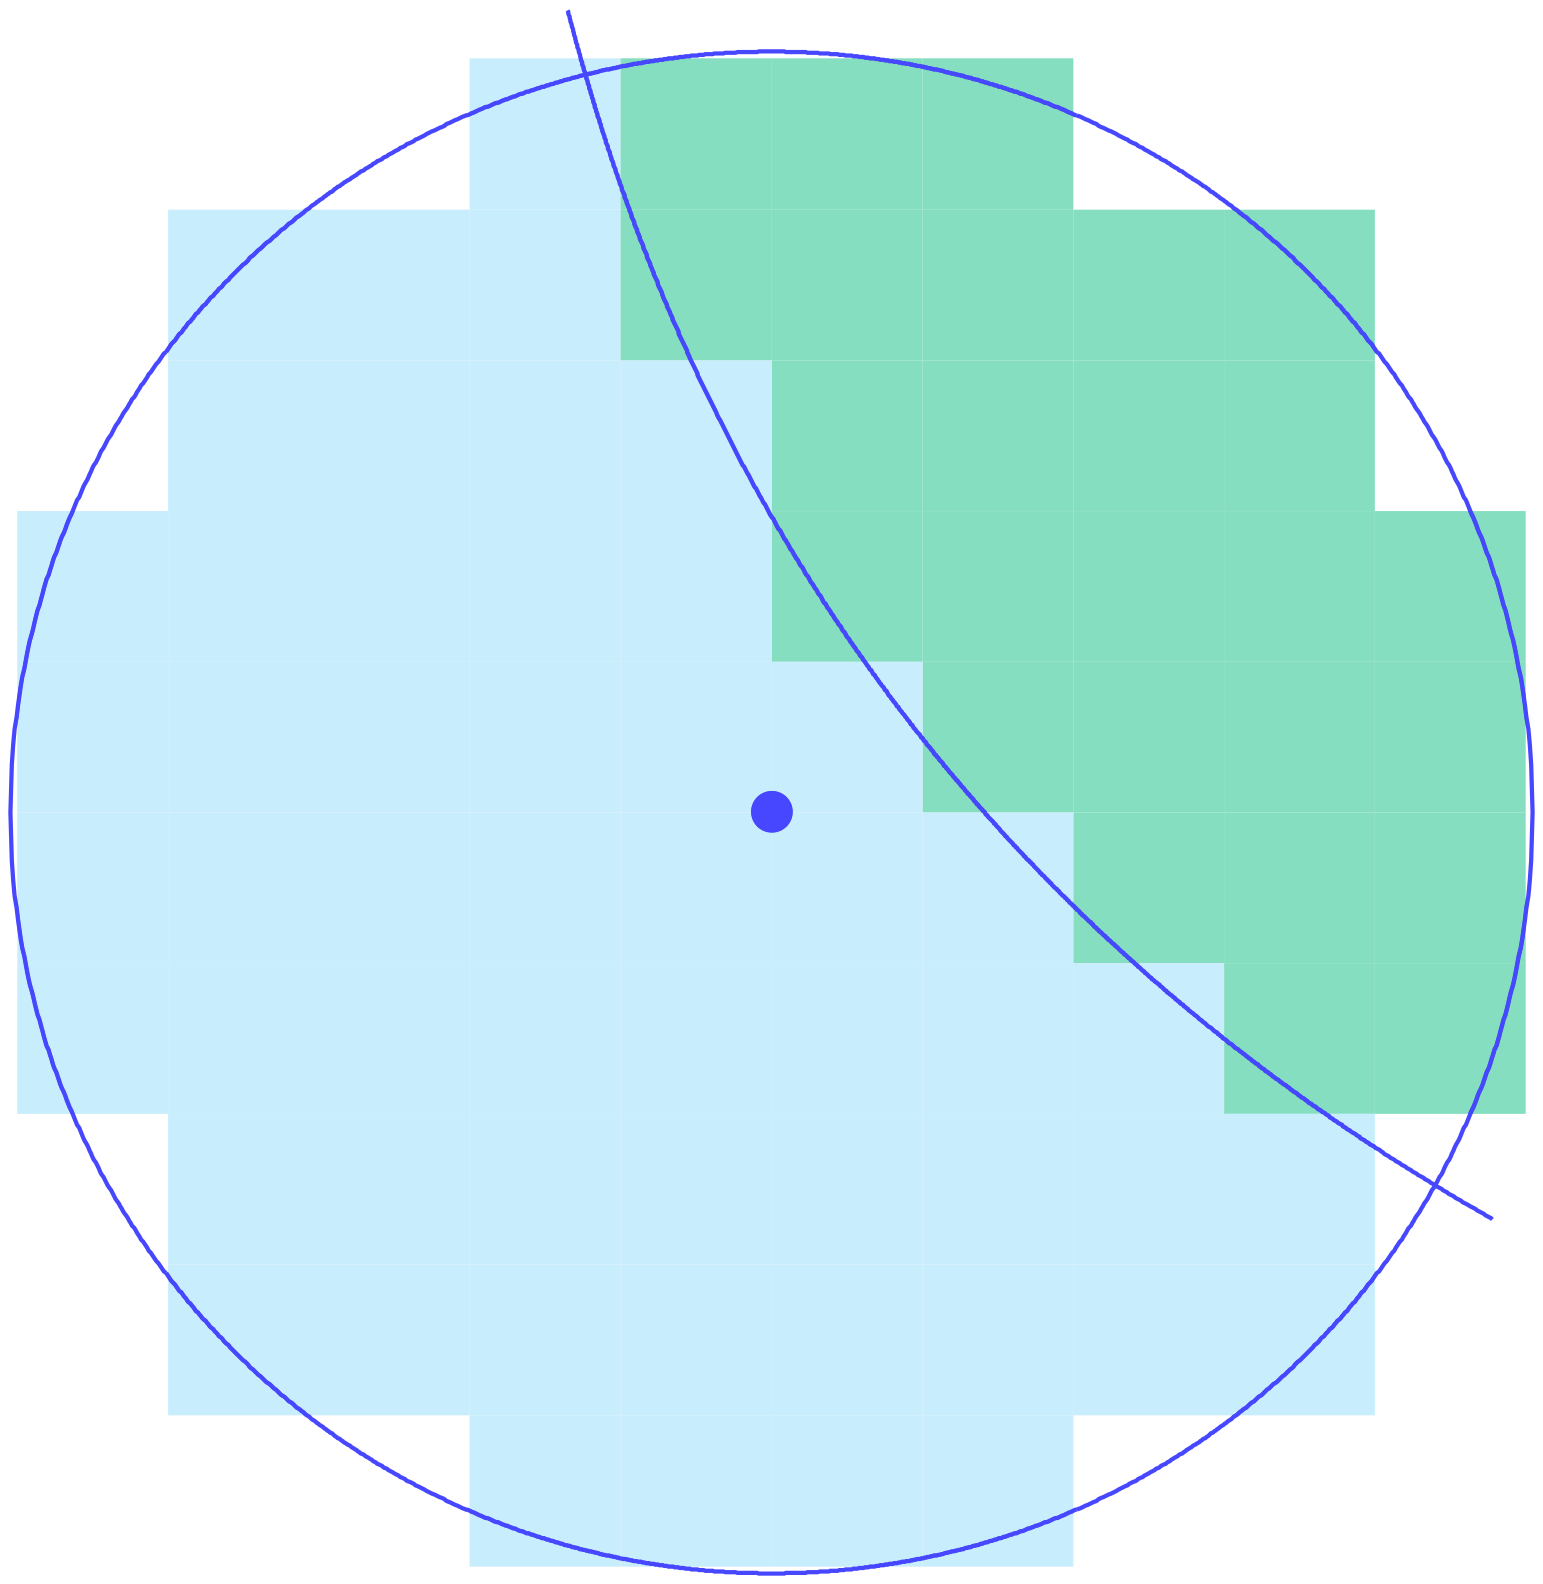
\includegraphics[scale=0.57]{media/2-shabaka/1-vor/dem2.png}
\label{fig:vor2}}
\subfigure[]{%
		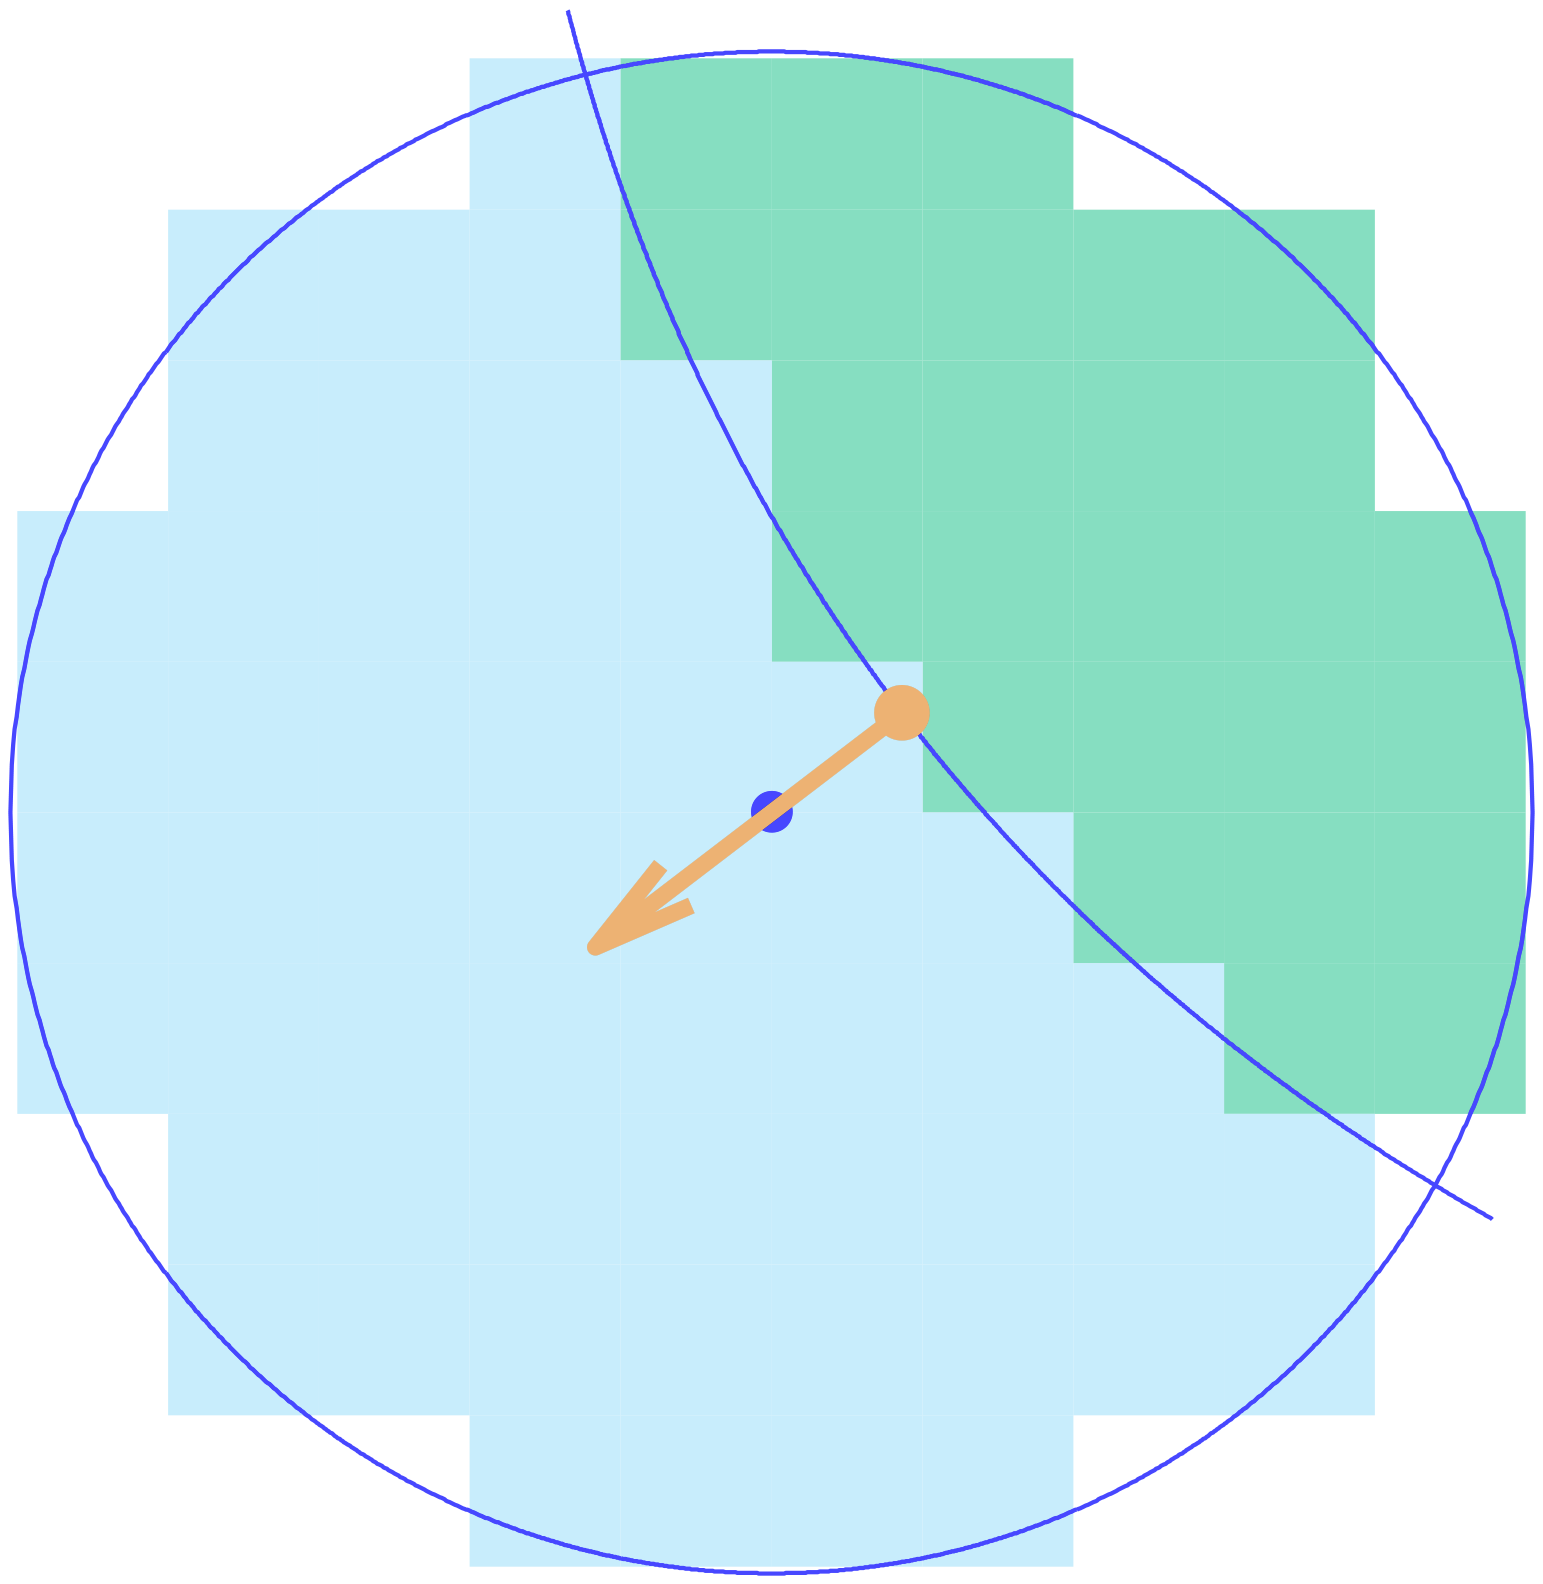
\includegraphics[scale=0.57]{media/2-shabaka/1-vor/dem3.png}
\label{fig:vor3}}
\subfigure[]{%
		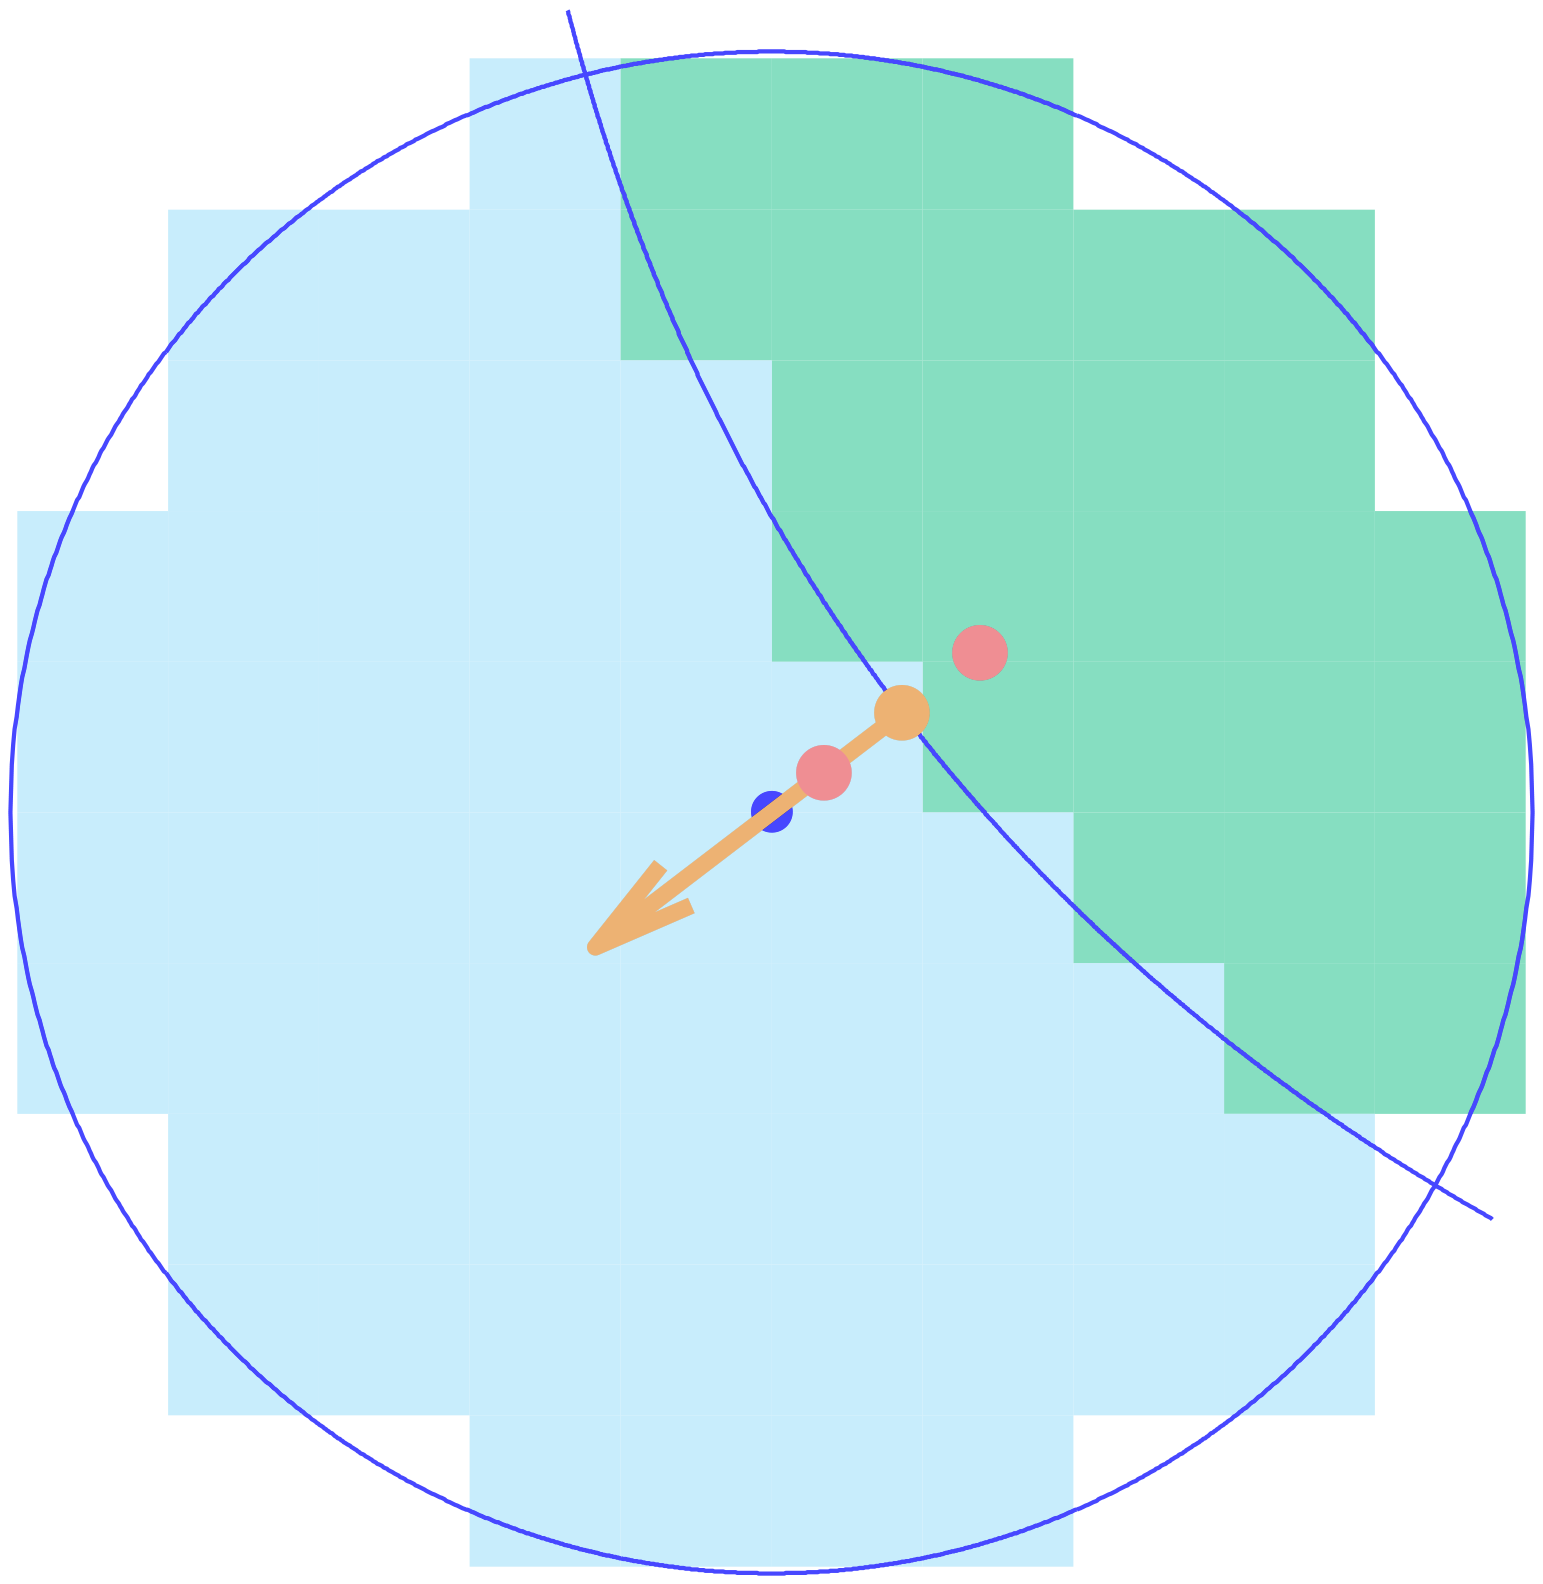
\includegraphics[scale=0.57]{media/2-shabaka/1-vor/dem4.png}
\label{fig:vor4}}
%
\caption{(a) Sampling window of segmented image, (b) interface approximation, (c) point/normal placement, and d) Voronoi site placement. Green voxels belong to the material of interest \textit{m} and blue voxels are void.}
\label{fig:vor}
\end{figure}

\begin{sidewaysfigure}[htbp!]
\centering
\subfigure[]{%
		
\includegraphics[scale=0.43]{media/vv/a1.png}
\label{fig:d2dvor1}}
\subfigure[]{%
		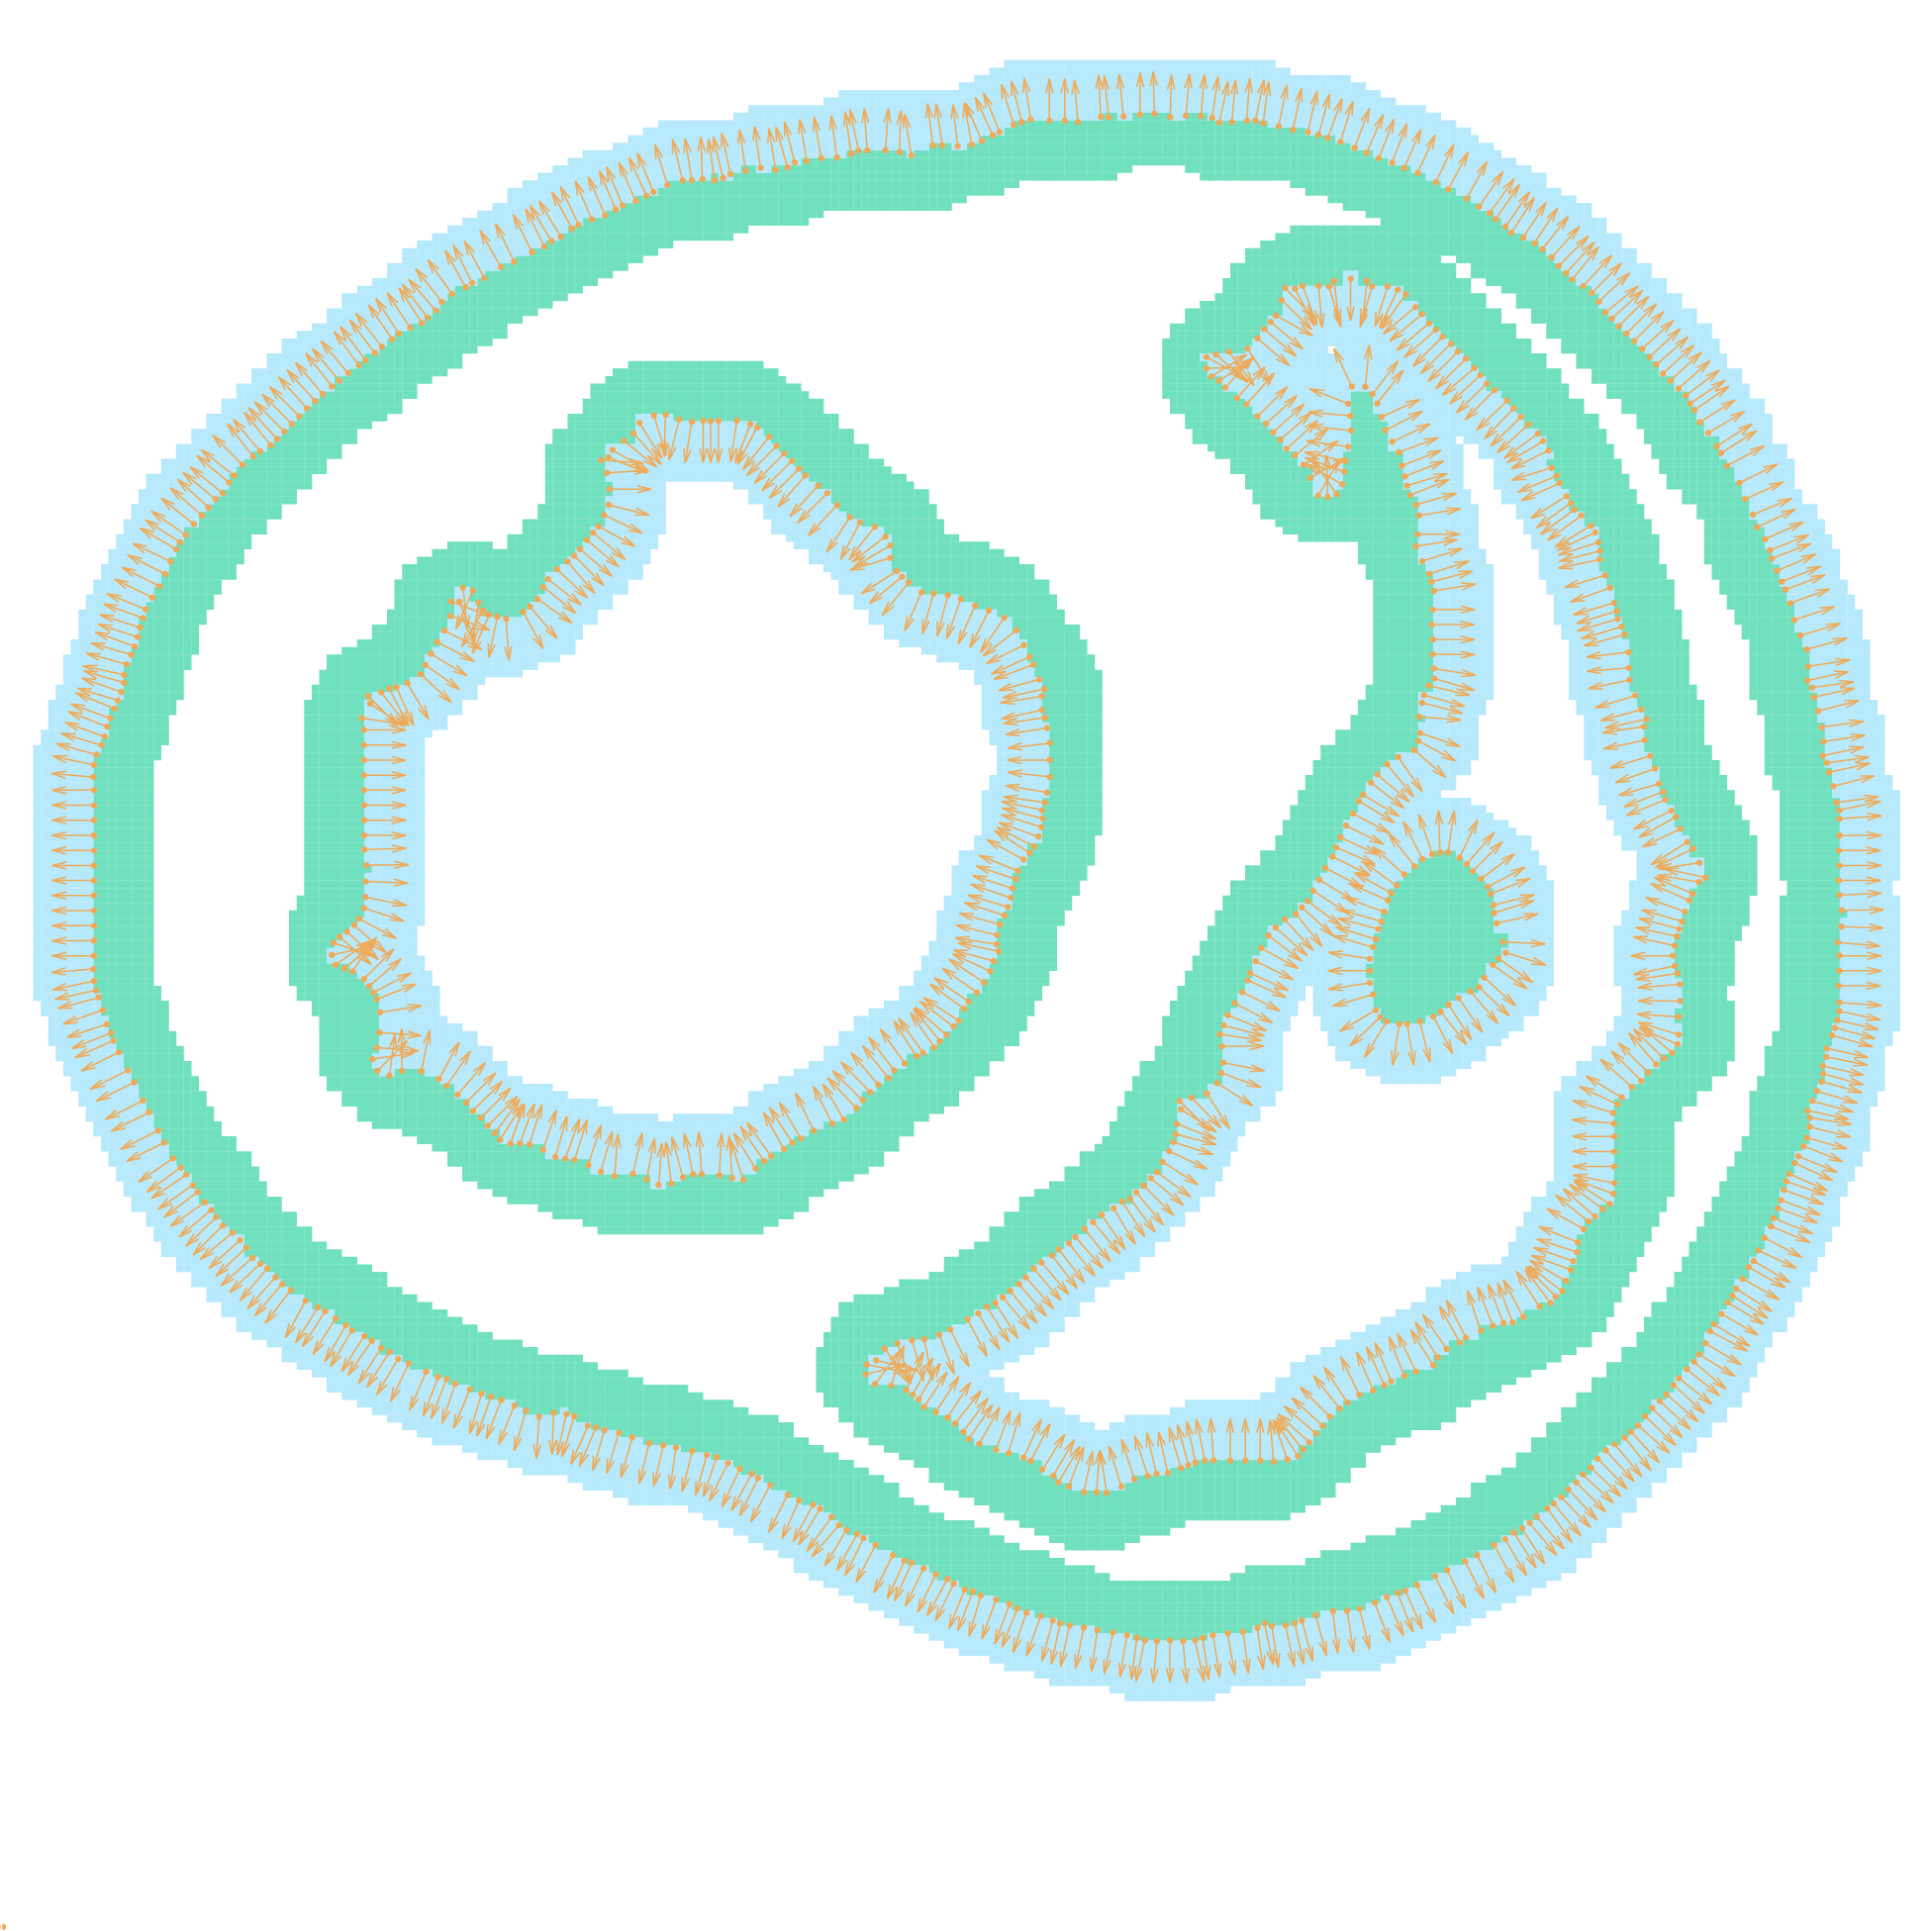
\includegraphics[scale=0.43]{media/vv/a2.png}
\label{fig:d2dvor2}}
\subfigure[]{%
		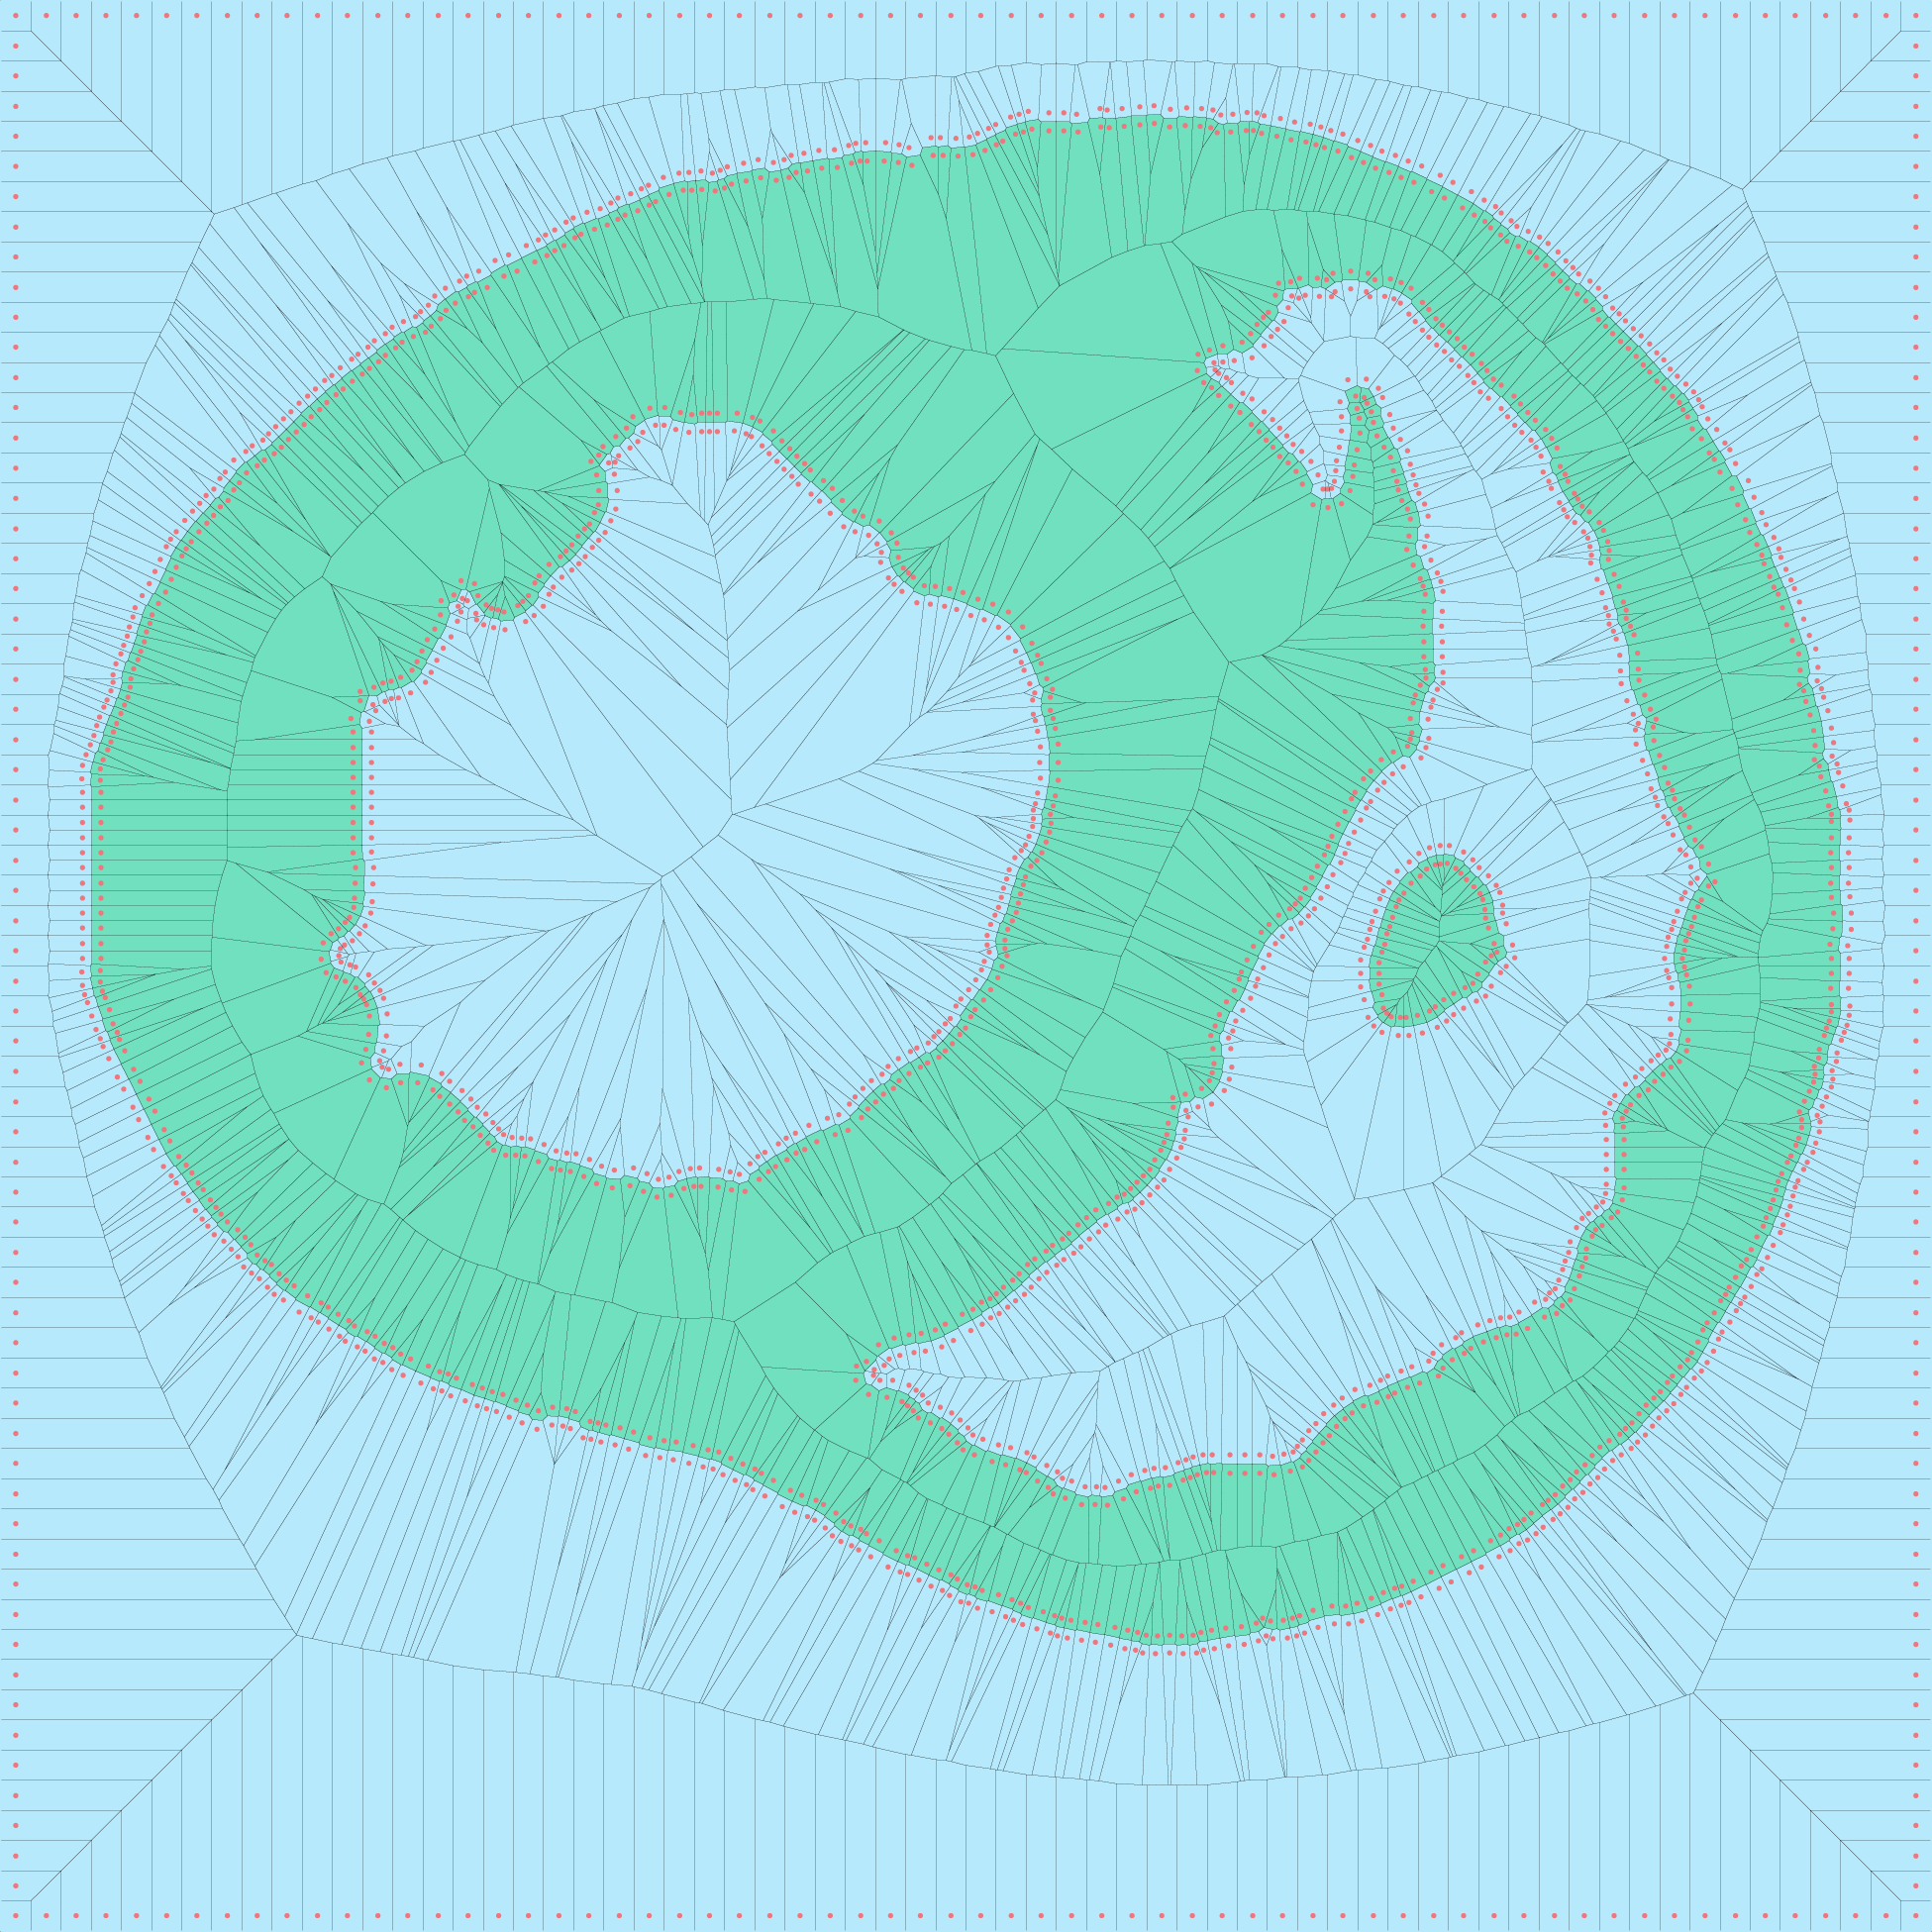
\includegraphics[scale=0.43]{media/vv/a3.png}
\label{fig:d2dvor3}}
%\subfigure[]{%
%		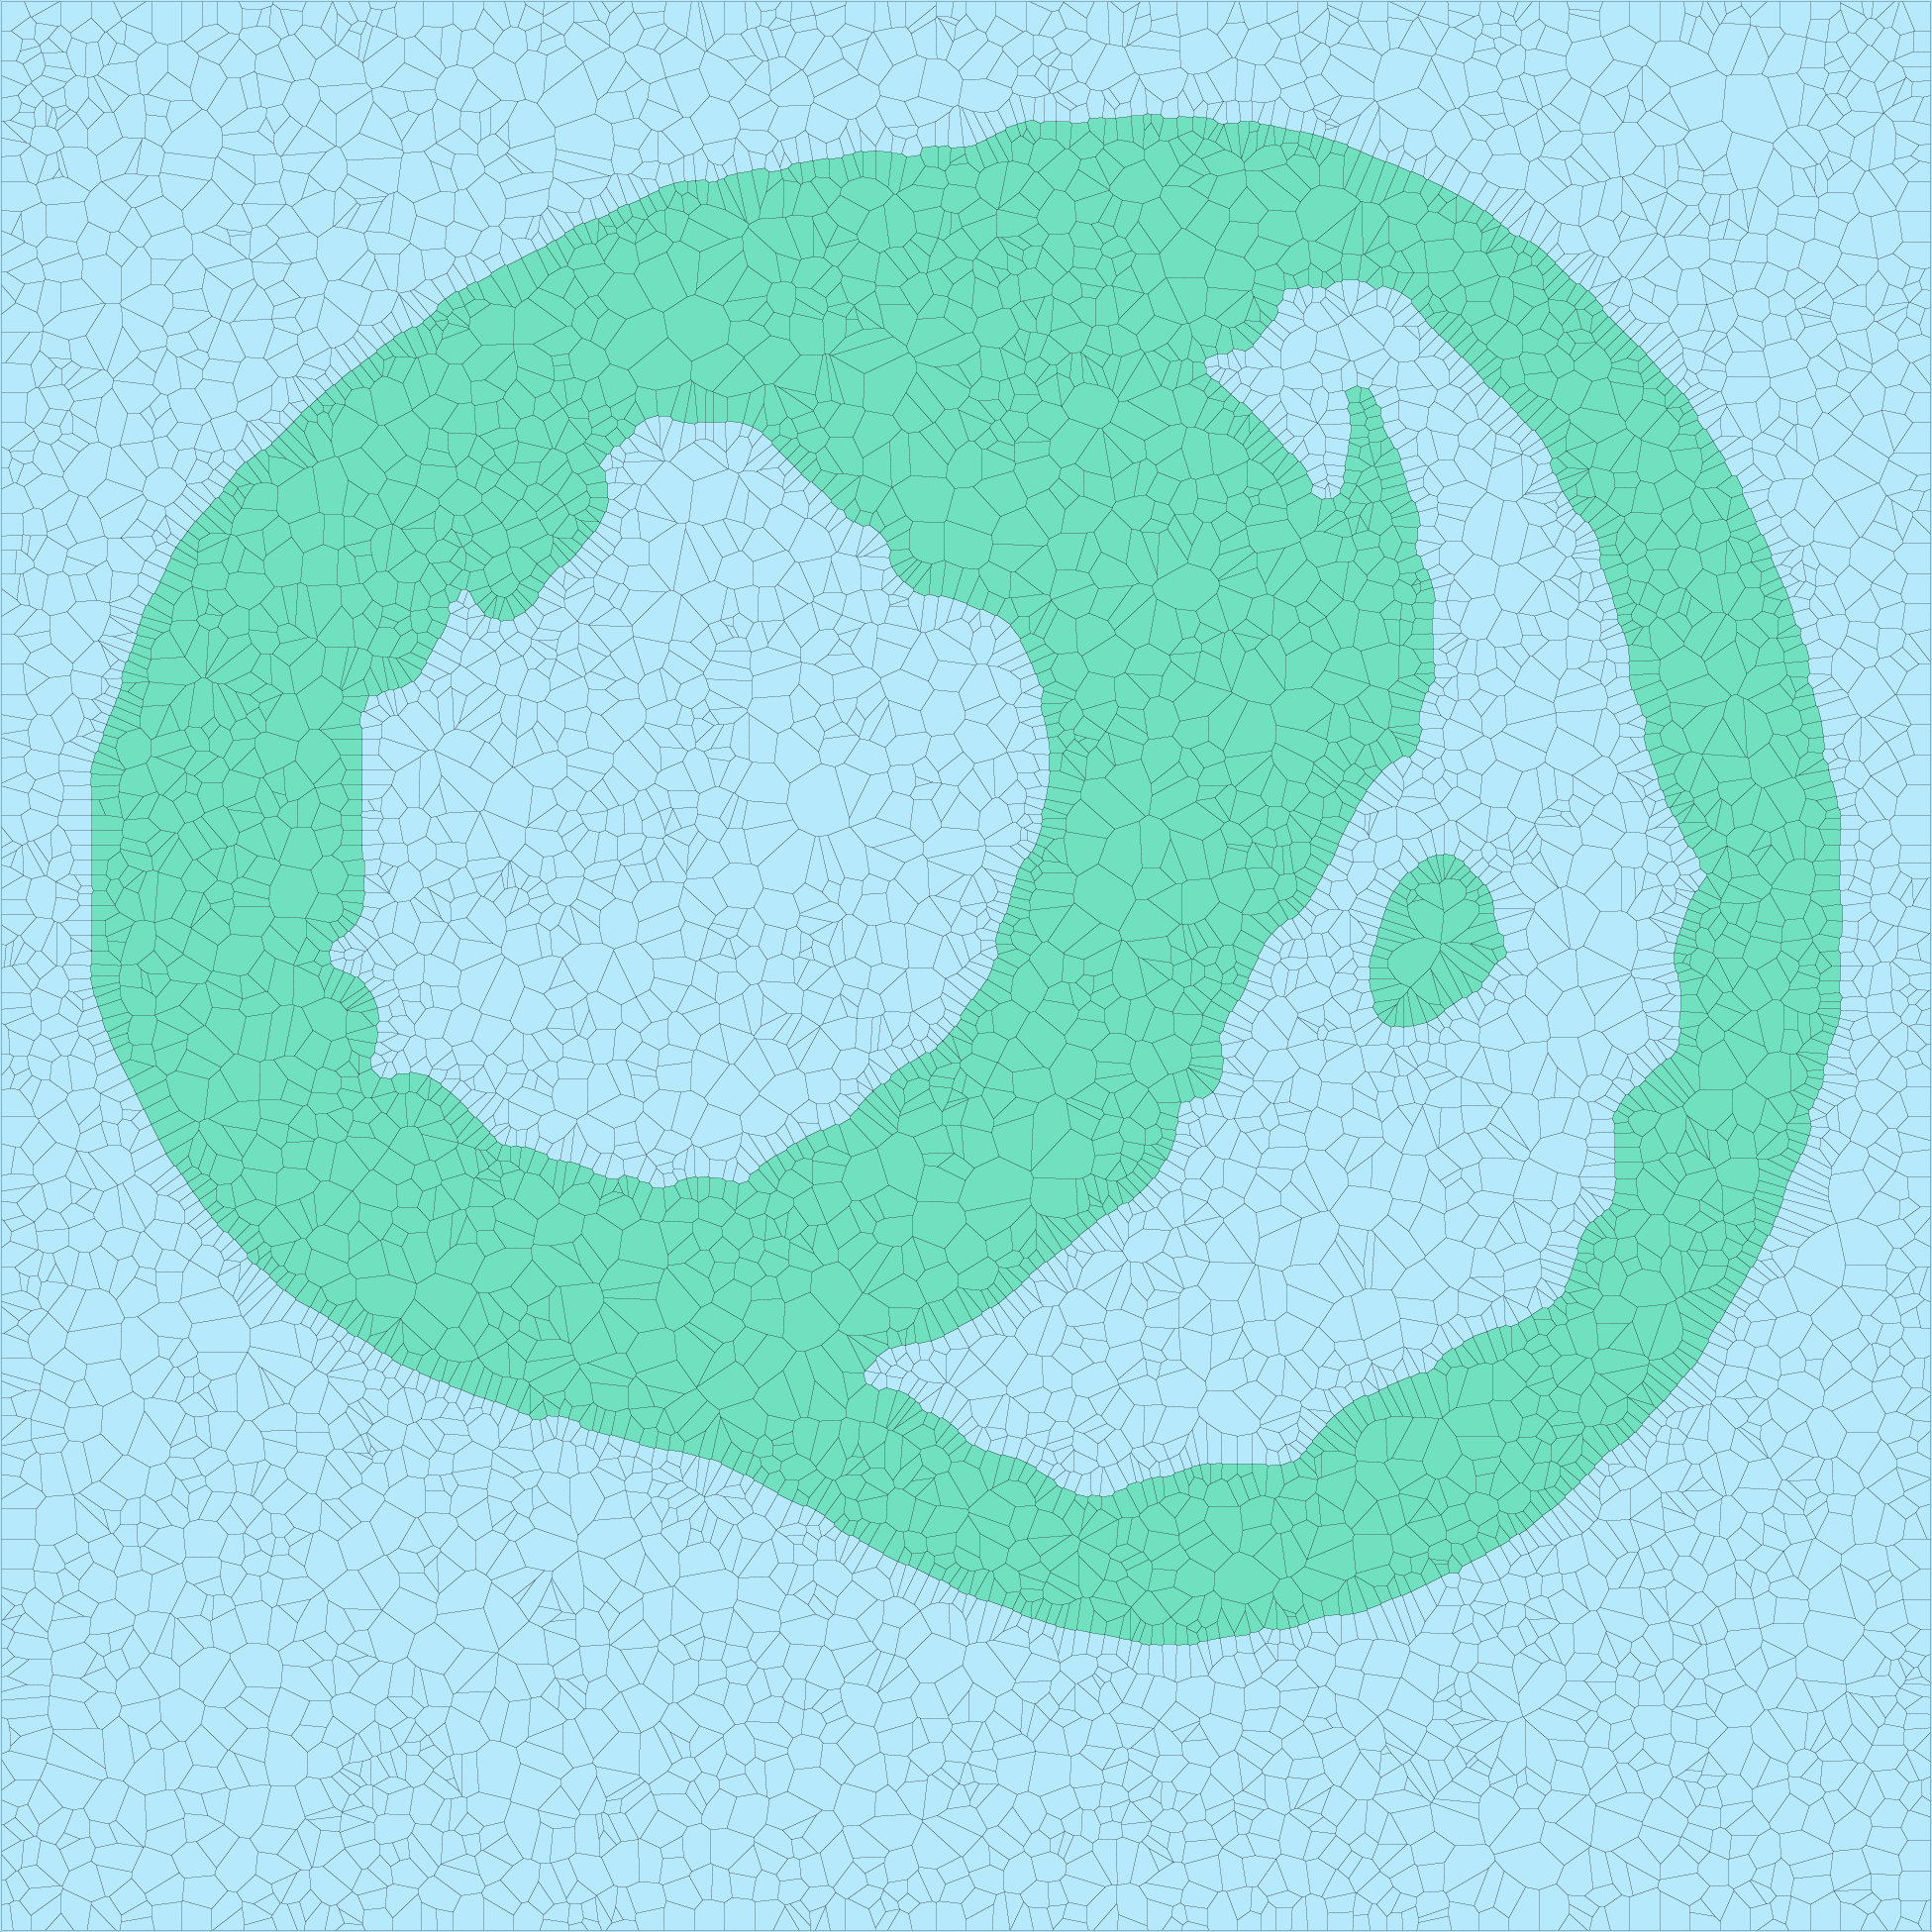
\includegraphics[scale=0.4]{media/vv/a4.png}
%\label{fig:d2dvor4}}
%
\caption{(a) Segmented image of 2D slice of \textit{ex vivo} canine heart, (b) resulting point cloud, and (c) Voronoi site placement and subsequent Voronoi partitioning and surface extraction}
\label{fig:d2dvor}
\end{sidewaysfigure}

\subsubsection{Window Selection}

Define the set of all voxels in a segmented image as $\mathcal{I}$. The segmented image  $\mathcal{I}$ is sampled with overlapping windows, each of which is a voxelized sphere with voxel radius $R_{\mathcal{W}}$. The sampling distance between adjacent windows is $d_{\mathcal{W}}$. The set of voxels in a particular window is defined as $\mathcal{W}$, and the number of voxels in that window is $n_{\mathcal{W}}$. Define the set of voxels in $\mathcal{W}$ that belong to the material of interest $m$ to be $\mathcal{M}$, and the number of voxels in $\mathcal{M}$ to be $n_{\mathcal{M}}$. A window $\mathcal{W}$ is deemed acceptable if it satisfies a threshold requirement. Define $k_{\mathcal{M}}$ as the ratio of voxels in $\mathcal{M}$ to the voxels in $\mathcal{W}$, i.e., $k_{\mathcal{M}} = n_{\mathcal{M}}/n_{\mathcal{W}}$. For a threshold value $\overline{k}_{\mathcal{M}}$, the window is discarded if $k_{\mathcal{M}} > \overline{k}_{\mathcal{M}}$ or $k_{\mathcal{M}} < 1 - \overline{k}_{\mathcal{M}}$. Thus, further calculations are only performed if there are enough voxels of both material \textit{m} and of void to justify approximating a material interface. Refer to~\tabref{window} for a list of these variables and their descriptions. 

\begin{table}[htbp!]
 \centering
   \begin{tabular}{|c||c|}
   \hline
   {\textbf{Variable}} & \textbf{Description} \\ \hline \hline
   $\mathcal{I}$ & set of all voxels in a segmented image \\ \hline
   $\mathcal{W}$ & set of all voxels in a window \\ \hline
   $m$ & material of interest \\ \hline
   {$k_{\mathcal{M}}$} & ratio of voxels in $\mathcal{M}$ to voxels in $\mathcal{W}$\\ \hline
   {$\overline{k}_{\mathcal{M}}$ \rule{0mm}{4mm}} & threshold value for $k_{\mathcal{M}}$ \\ \hline 
   $R_{\mathcal{W}}$ & window radius (in voxels) \\ \hline
   $d_{\mathcal{W}}$ & sampling distance between adjacent windows (in voxels) \\ \hline  
\end{tabular}
\caption{List of variables for window selection}
\label{tab:window}
\end{table}

\subsubsection{Interface Approximation}

For a particular window $\mathcal{W}$, we seek to approximate the interface between voxels belonging to $\mathcal{M}$ and voxels belonging to $\mathcal{W} \setminus \mathcal{M}$ by a surface $\mathcal{S}$. Assuming $\mathcal{W}$ has been deemed acceptable, an approximating sphere $\mathcal{D}$ of radius $R$ is defined, such that the center and volume of this sphere equal the center and volume of the window $\mathcal{W}$, respectively.

Define $\Omega_p$ as the physical space covered by the voxels belonging to $\mathcal{M}$. Define $\Omega$ as the physical space covered by an approximating lens to $\Omega_p$, determined by the space enclosed by the intersection of $\mathcal{D}$ and $\mathcal{S}$. The surface $\mathcal{S}$ is determined by minimizing the error between geometric properties of $\Omega$ and $\Omega_p$~(see~\figref{figure3}).

\begin{figure}[ht]
\centering
\subfigure[Window $\mathcal{W}$]{%
		
\includegraphics[scale=0.72]{media/om/dem2.pdf}
\label{fig:subfigure2}}
\subfigure[Approximating sphere $\mathcal{D}$]{%
		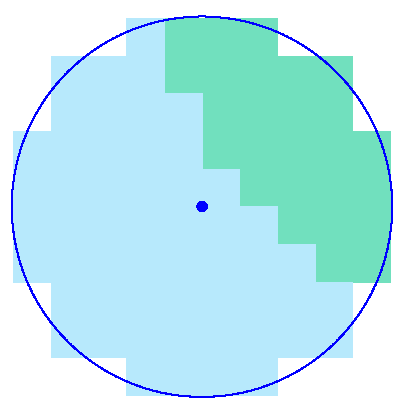
\includegraphics[scale=0.72]{media/om/dem3.pdf}
\label{fig:subfigure3}}

\subfigure[Approximating surface $\mathcal{S}$]{%
		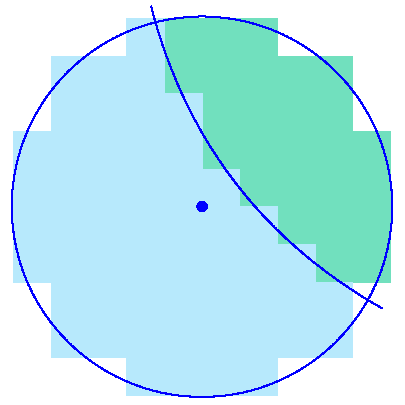
\includegraphics[scale=0.72]{media/om/dem4.pdf}
\label{fig:subfigure4}}
\subfigure[voxelized region $\Omega_p$]{%
		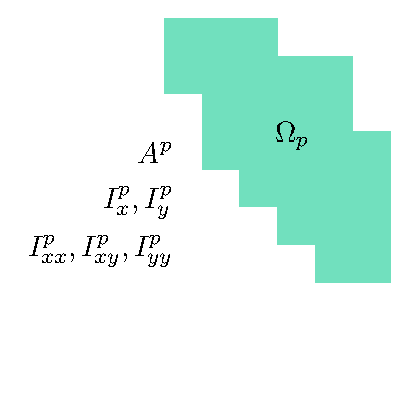
\includegraphics[scale=0.72]{media/om/omp.pdf}
\label{fig:subfigure5}}
\subfigure[Approximating lens $\Omega$]{%
		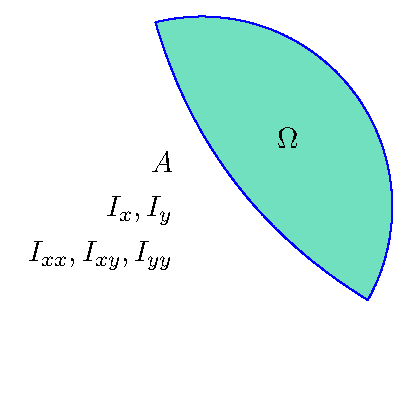
\includegraphics[scale=0.72]{media/om/om.pdf}
\label{fig:subfigure6}}

\caption{Interface approximation demonstrated in 2D}
\label{fig:figure3}
\end{figure}

The open surface $\mathcal{S}$ that approximates the interface takes an assumed form - for these purposes the interface is assumed a plane. If the center of the window is defined as the origin, the planar interface takes the form $x' = d$, where $(x',y',z')$ are the coordinates of a transformed coordinate system and $d$ is the perpendicular distance from the origin to the plane~(see~\figref{quad}).

\begin{figure}[ht!]
	\centering
		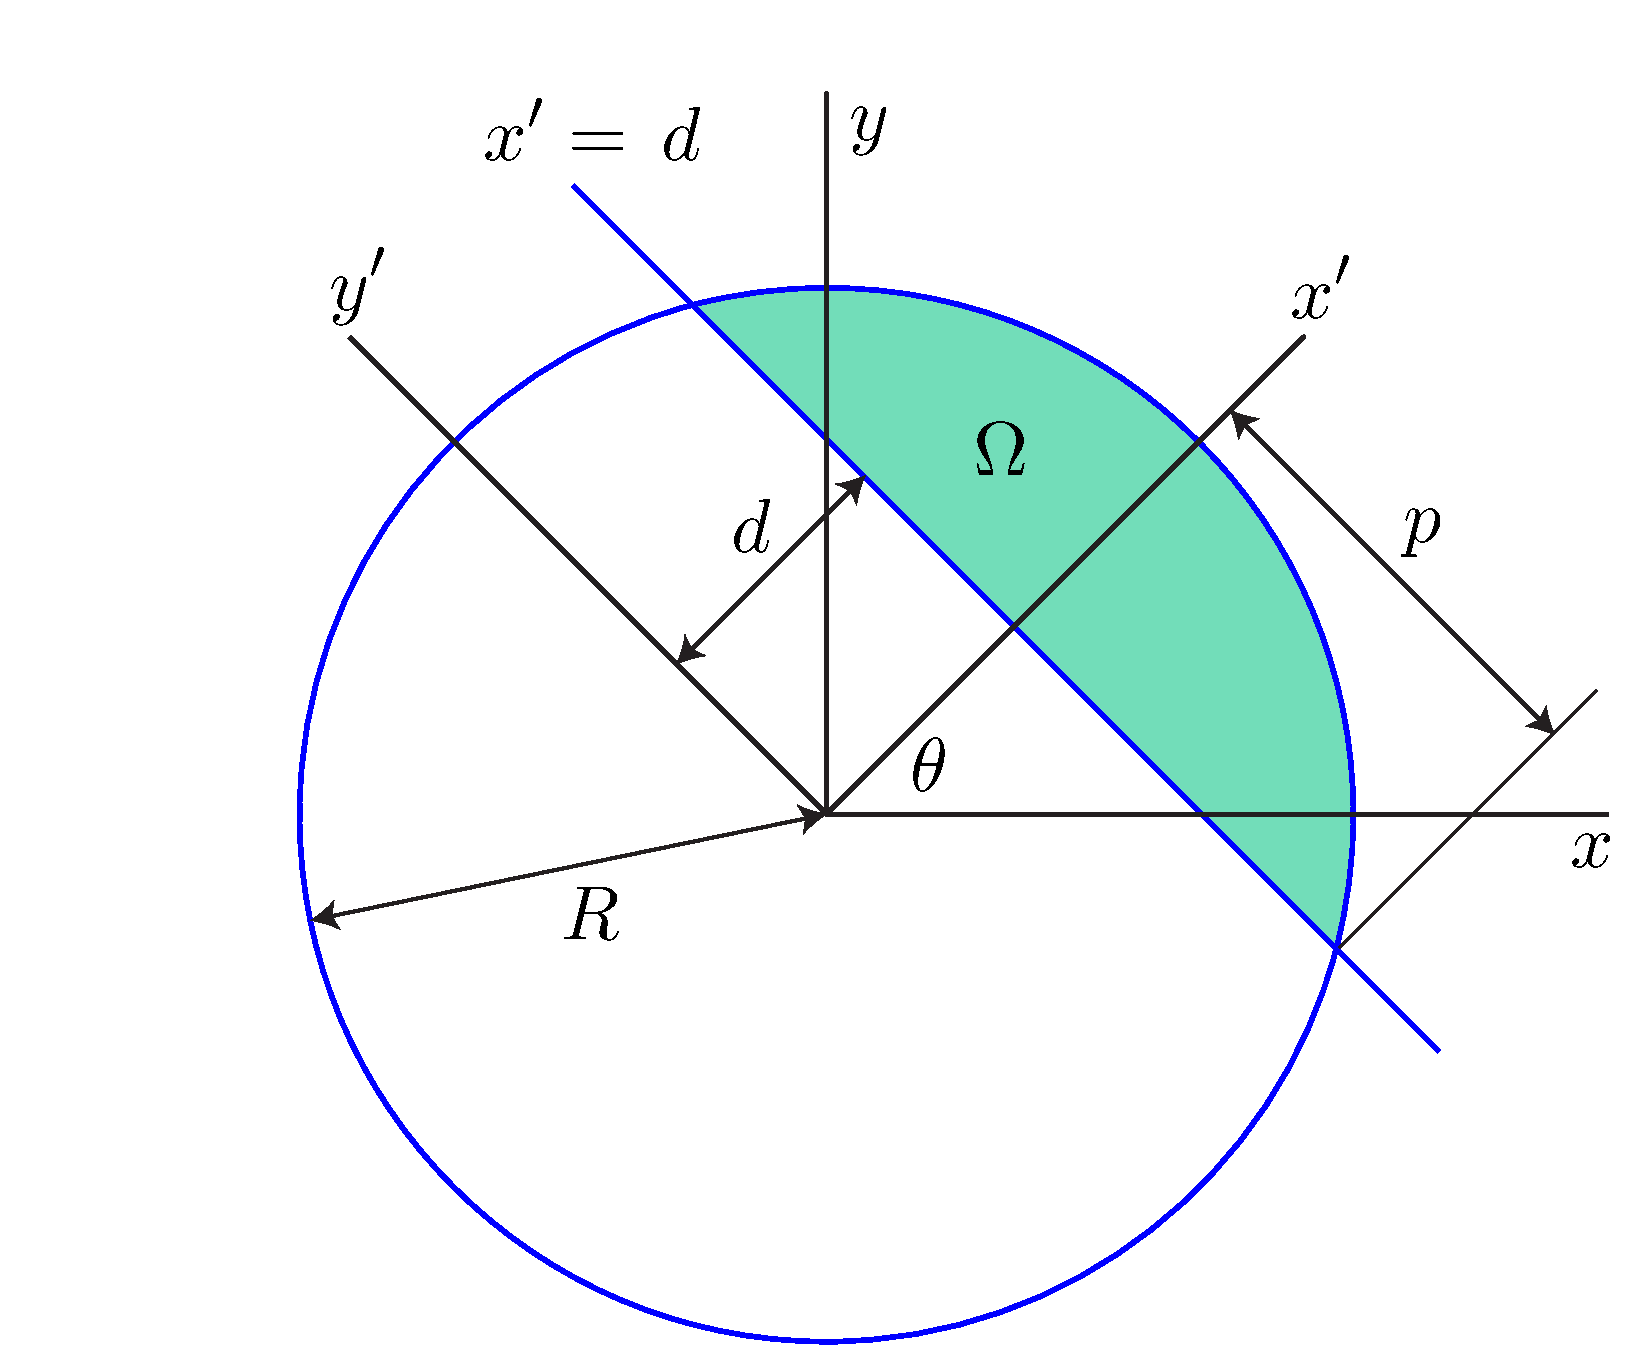
\includegraphics[scale=0.3]{media/om/window.pdf}
	\caption{Plane interface approximation demonstrated in 2D}
	\label{fig:quad}
\end{figure}

Define the following moments of volume for $\Omega_p$:
\begin{alignat}{5}
&{} &&V^p = \int_{\Omega_p}dv &&{} \\
I_{x\phantom{z}}^p &= \int_{\Omega_p}xdv, &&I_{y\phantom{z}}^p = \int_{\Omega_p}ydv, &&I_{z\phantom{z}}^p = \int_{\Omega_p}zdv \\
I^p_{xy} &= \int_{\Omega_p}xydv, &&I^p_{xz} = \int_{\Omega_p}xzdv, &&I^p_{yz} = \int_{\Omega_p}yzdv \\
I^p_{xx} &= \int_{\Omega_p}(y^2 + z^2)dv, \text{\ \ \ \ \ \ }&&I^p_{yy} = \int_{\Omega_p}(x^2 + z^2)dv, \text{\ \ \ \ \ \ }&&I^p_{zz} = \int_{\Omega_p}(x^2 + y^2)dv
\end{alignat}

The zeroth, first, and second moments of volume of $\Omega$ are defined in the same manner, with integrals performed over the domain of $\Omega$ instead.
%\begin{alignat}{5}
%&{} &&V = \int_{\Omega}dv &&{} \\
%I_{x\phantom{z}} &= \int_{\Omega}xdv, &&I_{y\phantom{z}} = \int_{\Omega}ydv, &&I_{z\phantom{z}} = \int_{\Omega}zdv \\
%I_{xy} &= \int_{\Omega}xydv, &&I_{xz} = \int_{\Omega}xzdv, &&I_{yz} = \int_{\Omega}yzdv \\
%I_{xx} &= \int_{\Omega}(y^2 + z^2)dv, \text{\ \ \ \ \ \ }&&I_{yy} = \int_{\Omega}(x^2 + z^2)dv, \text{\ \ \ \ \ \ }&&I_{zz} = \int_{\Omega}(x^2 + y^2)dv
%\end{alignat}
%For the purposes of computing an error functional, define the following quantities:
%\begin{alignat}{3}
%f^p &= V^p, \text{\ \ \ \ \ }&&f(d,\psi,\theta) = V \\
%\bm{g}^p &= \left[\begin{array} {ccc} {I_x^p} \\ {I_y^p} \\ {I_z^p} \end{array} \right], \text{\ \ \ \ \ }&&\bm{g}(d,\psi,\theta) = \left[\begin{array} {ccc} {I_x} \\ {I_y} \\ {I_z} \end{array} \right] \\
%\bm{h}^p &= \left[\begin{array} {ccc} {I_{xx}^p} & {-I_{xy}^p} & {-I_{xz}^p}\\ {-I_{xy}^p} & {I_{yy}^p} & {-I_{yz}^p} \\ -{I_{xz}^p} & {-I_{yz}^p} & {I_{zz}^p} \end{array} \right],\text{\ \ \ \ \ \ \ }&&\bm{h}(d,\psi,\theta) = \left[\begin{array} {ccc} {I_{xx}} & {-I_{xy}} & {-I_{xz}}\\ {-I_{xy}} & {I_{yy}} & {-I_{yz}} \\ -{I_{xz}} & {-I_{yz}} & {I_{zz}} \end{array} \right]
%\end{alignat}

Define the relative errors as:
\begin{align}
e_0(d,\psi,\theta) &=  \sqrt{\frac{(f - f^p)^2}{(f^p)^2}} \\
e_1(d,\psi,\theta) &=  \sqrt{\frac{(g_i - g_i^p)(g_i - g_i^p)}{g_j^{p}g_j^{p}}} \\
e_2(d,\psi,\theta) &=  \sqrt{\frac{(h_{ij} - h_{ij}^p)(h_{ij} - h_{ij}^p)}{h_{kl}^{p}h_{kl}^{p}}}
\end{align}
Finally, we define the relative error functional as follows:
\begin{align}
\mathcal{F}(d,\psi,\theta) = \beta_0e_0 + \beta_1e_1 + \beta_2e_2
\end{align}
where $e_0$, $e_1$, and $e_2$ are relative errors between the zeroth, first, and second order moments of volume of $\Omega_p$ and $\Omega$, respectively. They are functions of the interface parameters $d$, $\psi$, and $\theta$, where $\psi$ and $\theta$ are the yaw and pitch angles defining the plane. The values $\beta_0$, $\beta_1$, and $\beta_2$ are weighting coefficients, where $\beta_2 = 1 - \beta_0 - \beta_1$, and $\beta_i \in [0, 1]$. We seek the solution to the following unconstrained minimization problem: $\displaystyle \min_{d, \psi, \theta} \mathcal{F}(d,\psi,\theta)$, which can be solved by a variety of well-established techniques.

The moments of volume of $\Omega_p$ are computed based on a straightforward use of voxel dimensions and the parallel axis theorem. The moments of $\Omega$, on the other hand, are computed based on an intricate dependence on $d$, $\psi$, and $\theta$:
\begin{align}
p &= \sqrt{R^2 - d^2} \\
V^* &= 2\pi\left[-\frac{1}{2}dp^2 + \frac{1}{3}R^3 - \frac{1}{3}(R^2 - p^2)^{3/2} \right] \\
I^*_{x'x'} &= \frac{\pi}{30}\left[-15dp^4 + \sqrt{R^2-p^2}\left(12p^4 - 4p^2R^2 - 8R^4\right) + 8R^5 \right] \\
\begin{split}
I^*_{y'y'} &= \frac{\pi}{480}\Big[-160d^3p^2 + 128R^5 - \sqrt{R^2-p^2}\left(128R^4 - 96p^2R^2 - 32p^4\right) - 120dp^4 \Big]
\end{split}
\end{align}
\begin{align}
V &=  \begin{cases}
      V^*, & \text{if}\ d \geq 0 \\
      V^* + \frac{4\pi}{3}\left(R^2-p^2\right)^{3/2}, & \text{otherwise}
    \end{cases} \\
I_{x'} &= \frac{\pi}{4}\left[2p^2(R^2-d^2) - p^4 \right]\\
I_{y'} &= I_{z'} = 0 \\
I_{x'y'} &= I_{x'z'} = I_{y'z'} = 0 \\
I_{x'x'} &=  \begin{cases}
      I^*_{x'x'}, & \text{if}\ d \geq 0 \\
       I^*_{x'x'} + \frac{4\pi}{15}(R^2-p^2)^{3/2}(3p^2+2R^2), & \text{otherwise}
    \end{cases} \\
I_{y'y'} &=  \begin{cases}
     I^*_{y'y'}, & \text{if}\ d \geq 0 \\
     I^*_{y'y'} + \frac{2\pi}{15}(R^2-p^2)^{3/2}(p^2+4R^2), & \text{otherwise}
    \end{cases} \\
I_{z'z'} &= I_{y'y'}
\end{align}
Unsurprisingly, certain moments of volume exhibit symmetries in regard to the $y'$ and $z'$ axes. Note that additional terms may exist if $d$ is negative.

The geometric quantities are computed in the transformed coordinate frame and then transformed back to the original desired coordinate frame. This transformation is different for the zeroth, first, and second moments due to the different tensor rank for each of these quantities. Once the moments of $\Omega$ have been transformed to the original coordinate frame, they can be compared to those of $\Omega_p$. The first and second moments are transformed in the following manner (no transformation is required for the zeroth moment of volume):
\begin{align}
\bm{R} &= \left[\begin{array} {ccc} {\cos\psi\cos\theta} & {-\sin\psi} & {\cos\psi\sin\theta}\\ {\sin\psi\cos\theta} & {\cos\psi} & {\sin\psi\sin\theta} \\
{-\sin\theta} & {0} & {\cos\theta}\end{array} \right] \\
\left[\begin{array} {ccc} {I_x} \\ {I_y} \\ {I_z} \end{array} \right] &= \bm{R} \left[\begin{array} {ccc} {I_{x'}} \\ {I_{y'}} \\ {I_{z'}} \end{array} \right]\\
\bm{I}' &= \left[\begin{array} {ccc} {I_{x'x'}} & {-I_{x'y'}} & {-I_{x'z'}}\\ {-I_{x'y'}} & {I_{y'y'}} & {-I_{y'z'}} \\ -{I_{x'z'}} & {-I_{y'z'}} & {I_{z'z'}} \end{array} \right] \\
\bm{I} &= \left[\begin{array} {ccc} {I_{xx}} & {-I_{xy}} & {-I_{xz}}\\ {-I_{xy}} & {I_{yy}} & {-I_{yz}} \\ -{I_{xz}} & {-I_{yz}} & {I_{zz}} \end{array} \right] = \bm{R}\bm{I}'\mathbf{R}^T
\end{align}

With all relevant quantities defined, the \textit{subplex search method}~\cite{rowan} is used to minimize the error functional using an implementation in the package \textit{NLopt}~\cite{nlo}. The method is a \textit{derivative-free} method that is well suited for optimizing objective functions that are noisy or discontinuous. It was selected as the optimization approach due to the existence of square roots in the objective function, and the fact that robustness to a variety of inputs was the highest priority in developing the algorithm. A convergence tolerance $\varepsilon$ is defined such that on successive iterations, $\left| \mathcal{F}_{k+1} - \mathcal{F}_{k}\right| < \varepsilon$, where $k$ is the iteration number. For the specific examples and algorithm parameters to be discussed later in this chapter, convergence is achieved for each interface approximation after typically hundreds of iterations. This large value may be due to the admittedly tight tolerance value for $\varepsilon$ of $10^{-14}$, to nonlinearities or saddle points in the error functional not yet fully understood, or to inefficiencies in the nonlinear optimization tool used. However, because the point cloud generation step generates good results, and the entire process usually completes in less than one minute of wall clock time on a personal computer even for complex geometries, the convergence rate was not further explored as a means for improving the algorithm.

Finally, the solution is only accepted if the error functional is below a specified value $\overline{\mathcal{F}}$, i.e., $\Omega$ approximates $\Omega_p$ to a satisfactory degree. Specifically, we require that once convergence has been satisfied, the criterion $\mathcal{F} < \overline{\mathcal{F}}$ must also be met for the point and normal to be retained. In this way, outlier points for which the error minimization performs poorly are discarded. This typically occurs in regions of high curvature, where a plane does not approximate such an interface well. The point cloud is dense enough that simply discarding these points does not cause any discernible amount of under-sampling of the surface.

The solution to the minimization problem yields the values $d$, $\psi$, and $\theta$ that determine the optimal surface $\mathcal{S}$, from which the interface point and normal are defined. Refer to~\tabref{surface} for a summary of variables used in approximating the interface.

\begin{table}[htbp!]
 \centering
   \begin{tabular}{|c||c|}
   \hline
   {\textbf{Variable}} & {\textbf{Description}} \\ \hline \hline
   $\mathcal{D}$ & approximating sphere to $\mathcal{W}$ \\ \hline
   $\mathcal{S}$ & approximating surface to interface of interest \\ \hline      
   $R$ & radius of $\mathcal{D}$ \\ \hline   
   $\Omega_p$ & physical space covered by voxels belonging to $\mathcal{W}$ \\ \hline
   $\Omega$ & physical space covered by approximating lens of $\Omega_p$ \\ \hline      
   $(x,y,z)$ & axes aligned with image directions, whose origin is at the center of $\mathcal{W}$\\ \hline
   {$(x',y',z')$} & axes $(x,y,z)$ transformed such that $x'$ passes through centroid of $\Omega$ \\ \hline
%   {} & where $x'$ passes through the centroid of $\Omega$ \\ \hline   
   $d$ & perpendicular distance from center of $\mathcal{D}$ to plane $\mathcal{S}$  \\ \hline
   $\psi$ & yaw angle of rotation between $(x,y,z)$ and $(x',y',z')$ axes \\ \hline   
   $\theta$ & pitch angle of rotation between $(x,y,z)$ and $(x',y',z')$ axes \\ \hline
   $V^p$ & volume of $\Omega_p$ \\ \hline
   $I_{x}^p, I_y^p$ & first moments of volume of $\Omega_p$ \\ \hline     
   $I_{xy}^p, I_{xz}^p, I_{yz}^p$ & products of volume of $\Omega_p$ \\ \hline      
   $I_{xx}^p, I_{xy}^p, I_{yy}^p$ & second moments of volume of $\Omega_p$ \\ \hline
   $V$ & volume of $\Omega$ \\ \hline
   $I_{x}, I_y$ & first moments of volume of $\Omega$ \\ \hline
   $I_{xy}, I_{xz}, I_{yz}$ & products of volume of $\Omega$ \\ \hline   
   $I_{xx}, I_{xy}, I_{yy}$ & second moments of volume of $\Omega$ \\ \hline
   $e_0$ & relative error in zeroth moment of volume \\ \hline
   $e_1$ & relative error in first moment of volume \\ \hline
   $e_2$ & relative error in second moment of volume \\ \hline   
   $\beta_0$ & functional weighting coefficient for zeroth moment of volume error \\ \hline
   $\beta_1$ & functional weighting coefficient for first moment of volume error \\ \hline
   $\beta_2$ & functional weighting coefficient for second moment of volume error \\ \hline 
   $\varepsilon$ & convergence tolerance for minimization of functional $\mathcal{F}$ \\ \hline
   $\overline{\mathcal{F}}$ \rule{0mm}{4mm} & largest acceptable value of functional $\mathcal{F}$ \\ \hline        
\end{tabular}
\caption{List of variables for interface approximation}
\label{tab:surface}
\end{table}

\subsubsection{Interface Point and Normal Placement}

Once the parameters $d$, $\psi$, and $\theta$ are selected to fully define the surface that approximates the interface, a point location and outward normal are determined. The outward pointing normal is defined from the transformation of the $x$ axis to the $x'$ axis, i.e., the first column of matrix $\bm{R}$, and thus defined as such: $\bm{n} = -(\cos\psi\cos\theta,\text{\ }\sin\psi\cos\theta,\text{\ }-\sin\theta)$. With the origin at the center of sphere $\mathcal{D}$, the location of the interface normal is then simply $\mathbf{x}_p = -d\bm{n}$.

%%%%%%%%%%%%%%%%%%%%%%%%%%%%%%%%%%%%%%%%%%%%%%%
%%%%%%%%%%%%%%%%%%%%%%%%%%%%%%%%%%%%%%%%%%%%%%%
\subsection{Surface Reconstruction}
\label{Surface Reconstruction}

Surface reconstruction is the process of generating closed, manifold, polygonized surfaces from point clouds. The research found in the literature typically expects a dense, noisy population of points that are generated from laser-based scanners. The proposed algorithm does not in general produce a point cloud as dense as do laser scanners, but a brief review of surface reconstruction techniques is still informative.

Among the most well-known surface reconstruction algorithms are the \textit{Power Crust} and \textit{Poisson surface reconstruction} techniques. Amenta \textit{et al.}~\cite{amenta_2001} presented the \textit{Power Crust} algorithm for reconstructing watertight surfaces from unoriented point clouds. It first constructs the \textit{medial axis transform} from the point cloud, which is the set of maximal balls completely contained in the interior of the surface. The algorithm then applies an inverse transform to approximate the medial axis and produce a piecewise-linear surface. The algorithm does not perform well when the point set is not sufficiently dense. Also, it performs quite poorly for point clouds generated from the algorithm described in the previous section. Kazhdan \textit{et al.} presented \textit{Poisson surface reconstruction}~\cite{kazhdan_2008} and subsequently \textit{screened Poisson surface reconstruction}~\cite{kazhdan_2013} for oriented point clouds. They compute an indicator function defined as 1 for points inside the surface and 0 for points outside, whose gradient approximates the vector field defined by the oriented point cloud. This amounts to solving a Poisson problem for an implicit indicator function, followed by application of marching cubes to polygonize the surface. The \textit{screened} approach provides a soft constraint that encourages the reconstructed isosurface to pass through the input points. In practice, the screened approach is significantly more robust than the original approach in generating manifold surfaces from complex point clouds. The technique produces smooth surfaces that exhibit a resiliency to noise, outliers, and under-sampling that is superior to any other technique that has been experimented with.

Many other surface reconstruction approaches exist, including those making use of moving least squares, Delaunay and Voronoi constructions, and variational approaches~\cite{berger}. A novel Voronoi-based approach is presented as an alternative to these approaches that is tuned to address the type of noise and point density from the point cloud generation algorithm from the previous section.

The proposed surface reconstruction technique relies on constructing a \textit{Voronoi diagram}, which for our purposes is a nearest neighbor partitioning of $\mathbb{R}^3$ based on a set of input \textit{Voronoi sites}. The desired output from a Voronoi partition is a mesh - namely, a set of points, edges, facets, and cells (and their connectivities) that discretize space. Define a half-space $D(\bm{p},\bm{q})$ comprising all points $\bm{x}$ as close, or closer, to site $\bm{p}$ than to site $\bm{q}$:
\begin{equation}
D(\bm{p},\bm{q}) = \{\bm{x} \mid d(\bm{p},\bm{x}) \leq d(\bm{q},\bm{x})\}
\end{equation}
where a distance function $d$ must be defined. Although there are instances of more exotic distance functions leading to modified Voronoi approaches, the distance function for standard Voronoi diagrams is simply the Euclidean distance. The \textit{Voronoi cell} $V(\bm{p})$ associated with site $\bm{p}$ is the intersection of all half-spaces involving site $\bm{p}$ and all other sites $\bm{q}$ belong to the set $\mathcal{P}$:
\begin{equation}
V(\bm{p}) = \bigcap \limits_{\bm{q} \in \mathcal{P}, \bm{q} \neq \bm{p}} D(\bm{p},\bm{q})
\end{equation}
A number of important properties exist for Voronoi partitions and their dual \textit{Delaunay tessellations}. For these purposes, though, the most important property is that the surface extracted from a set of Voronoi cells connected by shared facets is watertight and manifold. Several important considerations must be made in constructing a Voronoi partition, including degenerate and near-degenerate cases, the data schema and order of construction of the connected polytopes, and the
performance of the algorithm. Refer to Aurenhammer~\cite{aurenhammer_1991} for a detailed survey of the mathematical and algorithmic approaches to Voronoi diagrams.

The proposed technique involves the following steps, to be described in turn:
\begin{itemize}[noitemsep]
\item Generate Voronoi site set from oriented point cloud and perform Voronoi partition of image
\item Define b-rep as the set of facets that share Voronoi sites with different material types, and perform cleanup on that surface
\item Decimate (coarsen) the surface to a more tractable mesh resolution
\end{itemize}

\subsubsection{Voronoi Site Generation and Voronoi Partitioning}

Given the location of an interface point $\bm{x}_p$ and orientation of its corresponding normal $\bm{n}$, two Voronoi sites are placed on either side of the point along the line of action of the normal, as shown in~\figref{vor4} and~\figref{d2dvor3}. They are separated from the point by a distance $b$, and thus their locations are $\bm{x}_p \pm b \bm{n}$. The two Voronoi sites are assigned material types. For the two-material case considered here, the site corresponding to the position $\bm{x}_p - b\bm{n}$ is inside $\Omega$, and thus is assigned material $m$. The site corresponding to the position $\bm{x}_p + b\bm{n}$ is outside $\Omega$, and thus is assigned a void material. \textit{Voronoi partitioning} is performed using an implementation from \textit{Qhull}~\cite{barber_1996}, that is robust even for near-degenerate Voronoi site locations.

\subsubsection{Surface Extraction and Cleanup}

The b-rep is extracted from the Voronoi partition as the set of facets that share Voronoi sites of differing material types. An additional step is performed, however, to mitigate undesired ``cross-talk'' facets caused by Voronoi partitioning of neighboring site pairs. ``Good facets'' are identified as those b-rep facets whose Voronoi sites belong to a site pair originating from the same point and normal, and ``bad facets'' are those b-rep facets whose Voronoi sites originate from different points in the point cloud. For surfaces with small curvature, the area of good facets significantly outweighs that of the bad facets. Nonetheless, the existence of bad facets causes a stair-stepping feature in the resulting surface that is unacceptable.

The artifact is addressed as follows: ``bad edges'' are identified as those edges that share two bad facets. Networks of connected bad edges are identified, and each network is collapsed to one point (see \figref{cross1}). For surfaces with a small amount of curvature, no bad edges are connected, and thus each is independently collapsed. Any good facet that is connected to a network of bad edges is modified to connect to the new collapsed point. The good facets are triangulated to maintain planarity following the removal of bad facets. This increases the data required to define the surface mesh, but the decimation step described in the next section resolves this issue immediately. The sequence is demonstrated on the full \textit{ex vivo} heart example in~\figref{cross2}.

\begin{sidewaysfigure}[htbp!]
\centering
\subfigure[]{%
		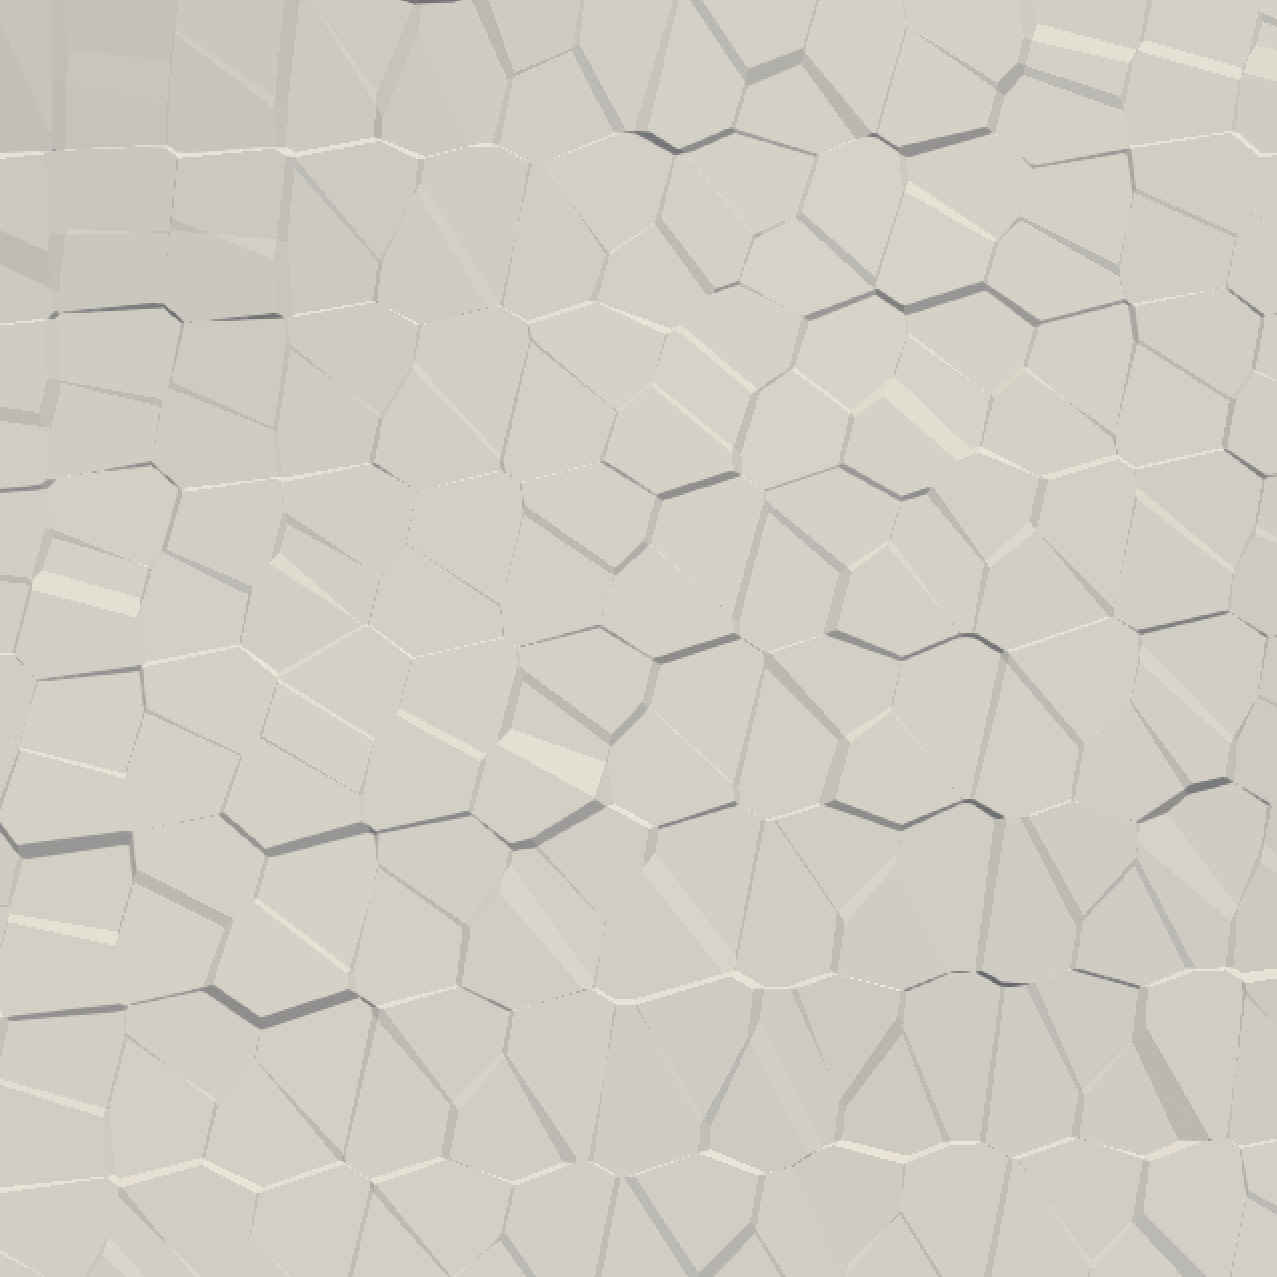
\includegraphics[scale=0.11]{media/2-shabaka/3-clean-zoom/1-init-zoom.png}
\label{fig:cross1-1}}	
\subfigure[]{%
		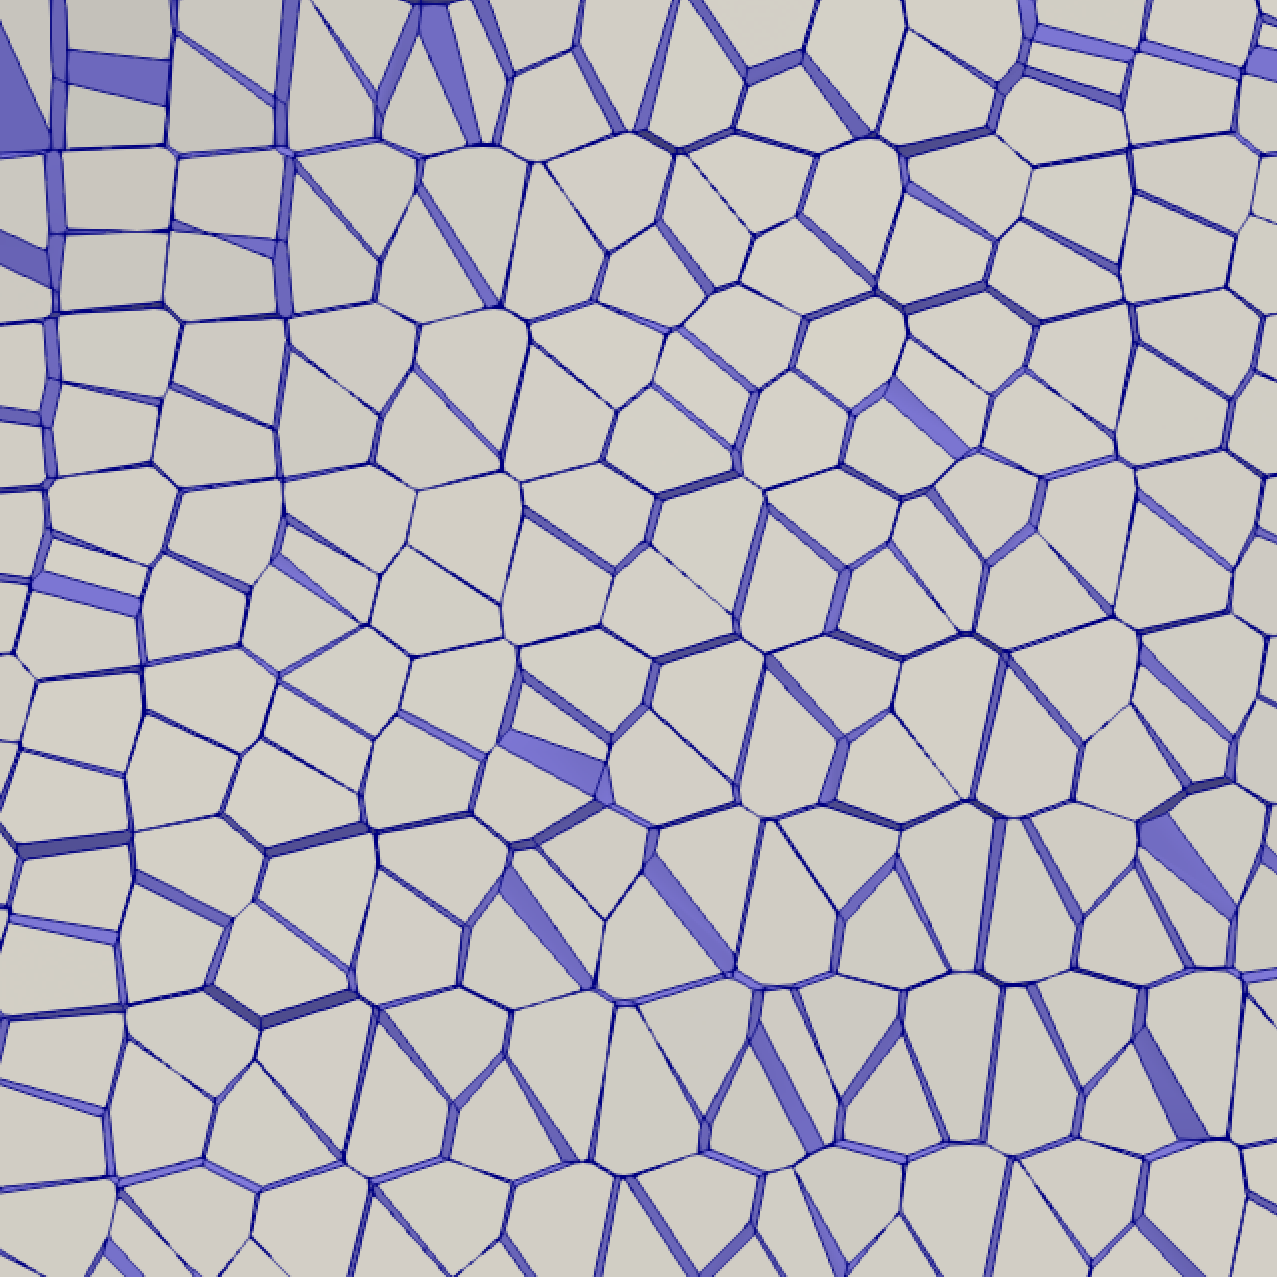
\includegraphics[scale=0.11]{media/2-shabaka/3-clean-zoom/2-badfacets-zoom.png}
\label{fig:cross1-2}}
\subfigure[]{%
		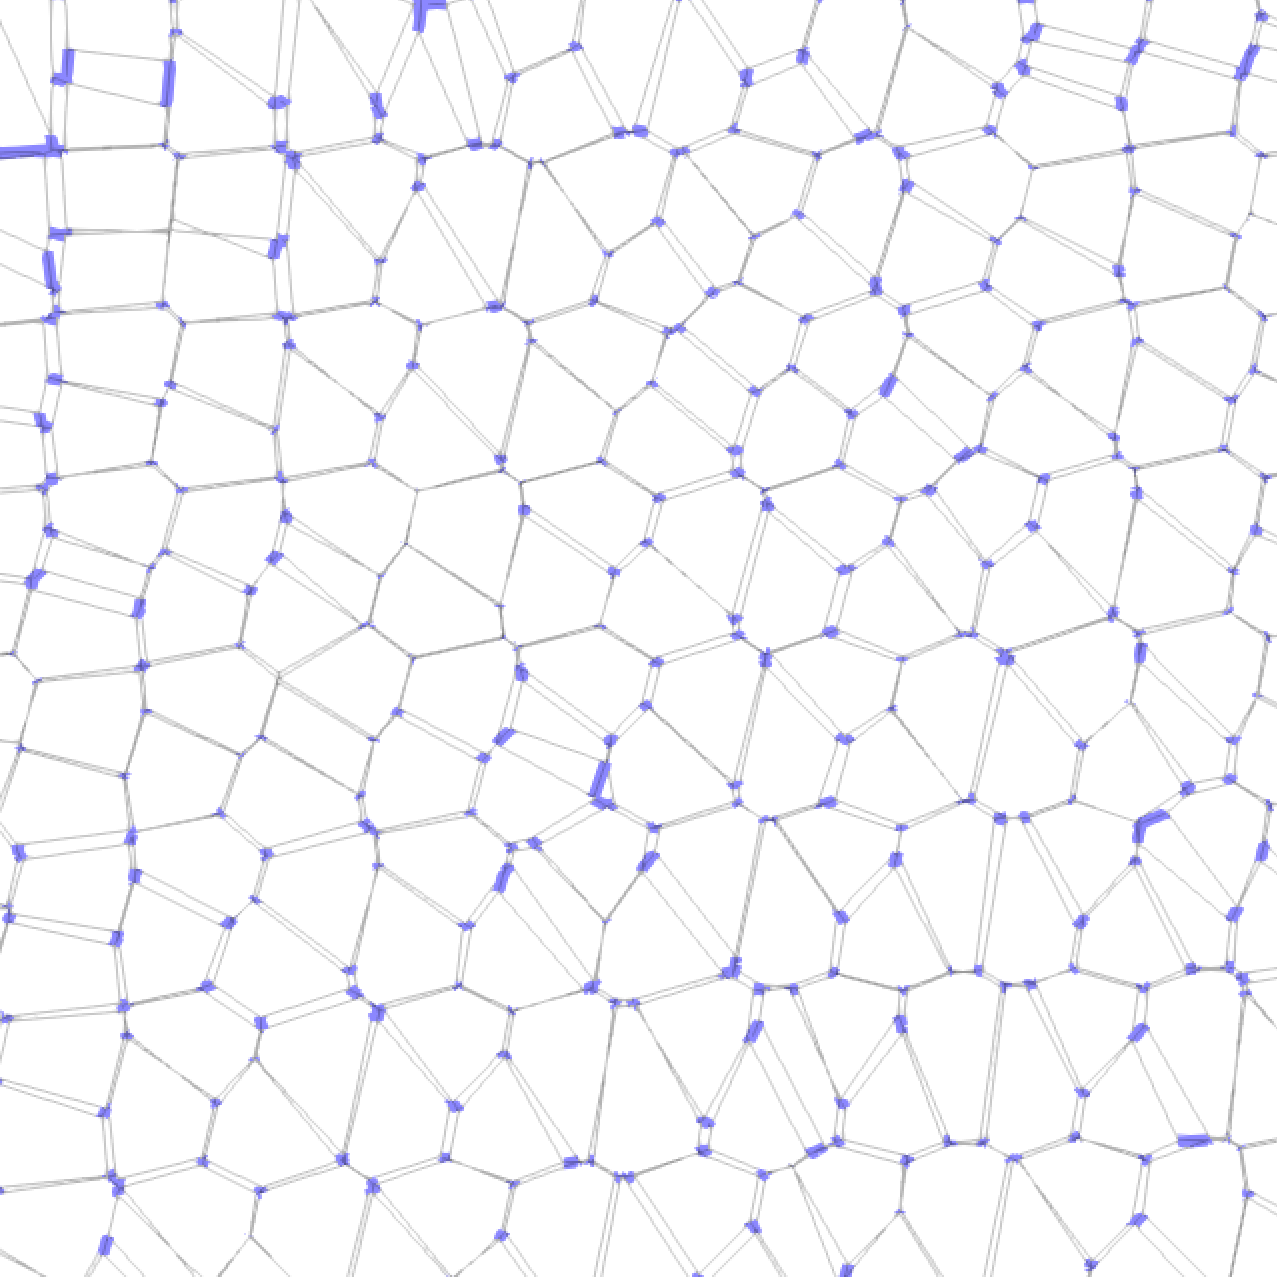
\includegraphics[scale=0.11]{media/2-shabaka/3-clean-zoom/3-badsegs-zoom.png}		
\label{fig:cross1-3}}
\subfigure[]{%
		
\includegraphics[scale=0.11]{media/2-shabaka/3-clean-zoom/4-fine-zoom.png}
\label{fig:cross1-4}}				
%
\caption{Clean-up of undesirable ``cross-talk'' facets for a surface patch: (a) initial surface following Voronoi-based surface reconstruction, (b) identification of ``cross-talk'' facets, (c) identification of edges to be collapsed, (d) final cleaned surface}
\label{fig:cross1}
\end{sidewaysfigure}

For the vast majority of bad edge networks, the collapse technique results in a smoother surface that remains closed and manifold. For regions of high-curvature, there is a small set of cases in which the clean-up step may cause the surface to become non-manifold. The topology of particular networks of bad edges that cause this phenomenon are identified based on heuristics. These networks are not collapsed to preserve the manifold property. The current approach thus does not capture regions of high curvature well during the point cloud generation step, and furthermore is unable to alleviate the issue of ``cross-talk'' facets in regions of high curvature. Fortunately, these remaining artifacts are small enough that the ensuing decimation step removes them.

Handling regions of curvature or even sharp corners and edges can certainly be done, though. The technique would involve including additional templates in the interface approximation step that would allow more than two Voronoi sites to be generated for each sampling window. For example, three Voronoi sites can be used to produce an edge, and four sites can be used to produce a corner. This would significantly improve the point cloud approximation of the underlying surface, perhaps to a degree that the collapsing technique described would remove all cross-talk facets with no concern of losing manifoldness.

\begin{sidewaysfigure}[htbp!]
\centering
\subfigure[]{%
		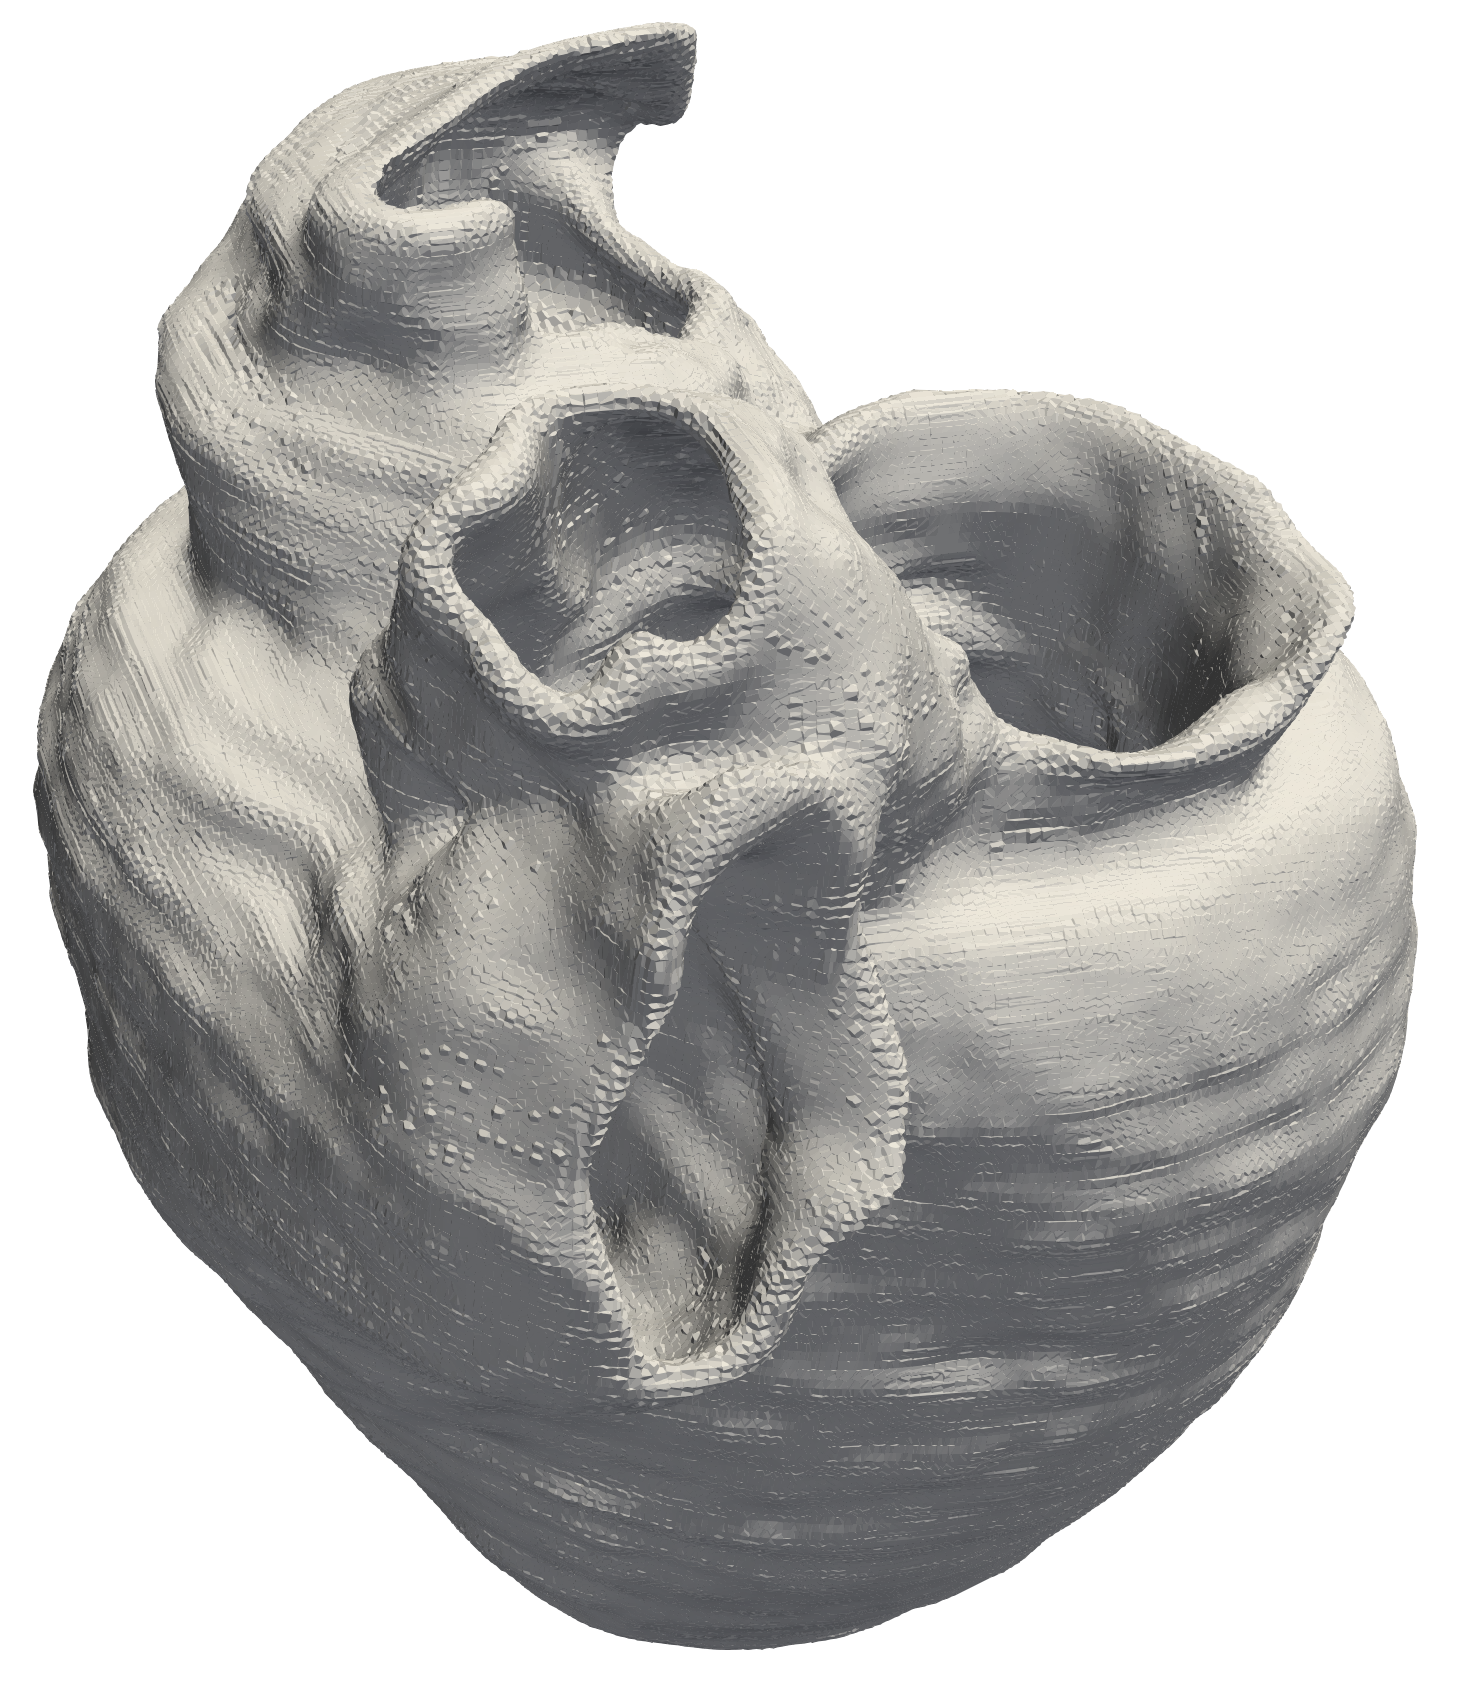
\includegraphics[scale=0.1]{media/2-shabaka/4-clean/1-init.png}
\label{fig:cross2-1}}		
\subfigure[]{%
		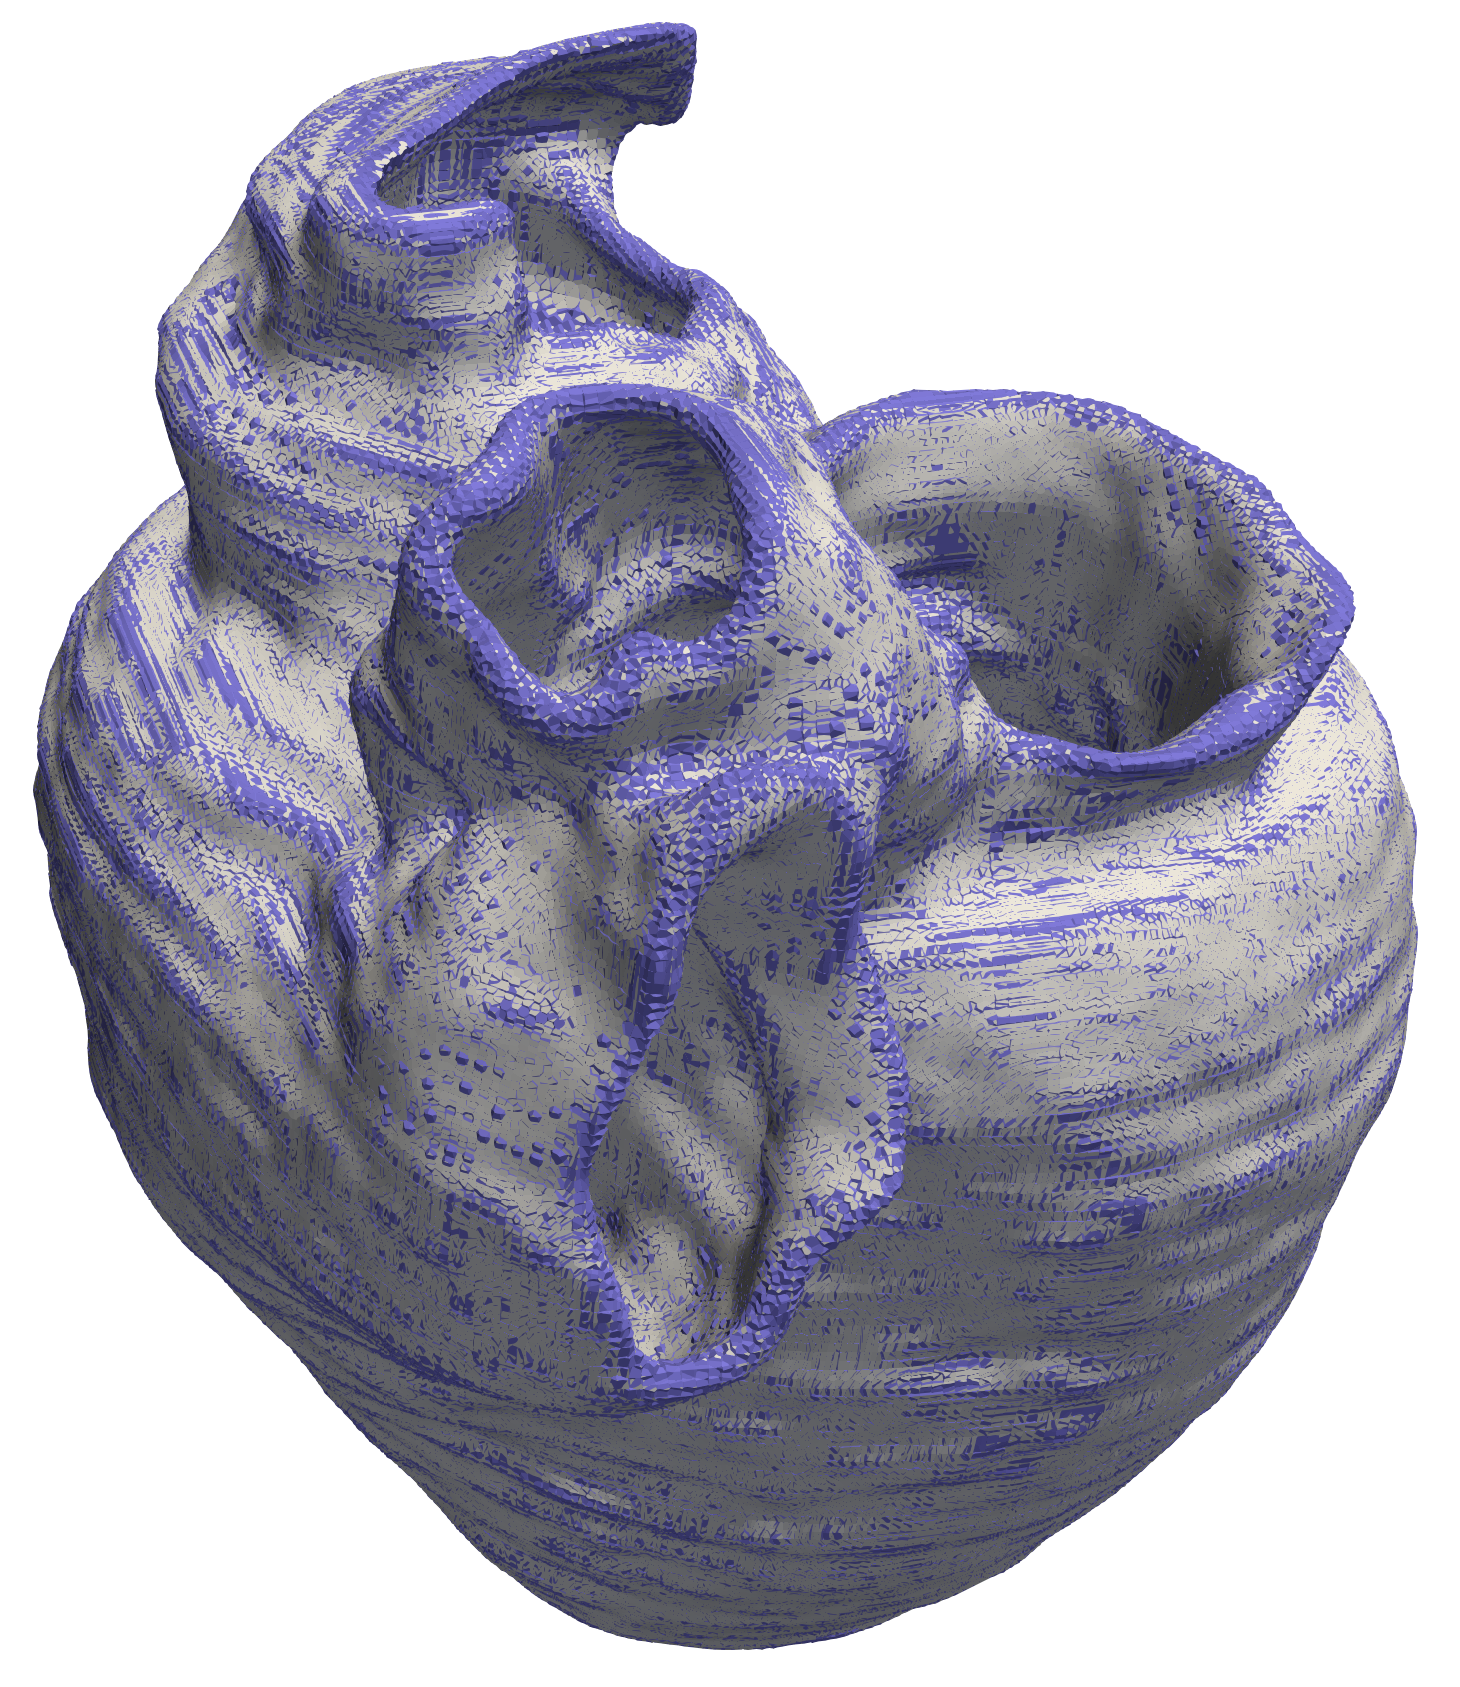
\includegraphics[scale=0.1]{media/2-shabaka/4-clean/2-badfacets.png}
\label{fig:cross2-2}}		
\subfigure[]{%
		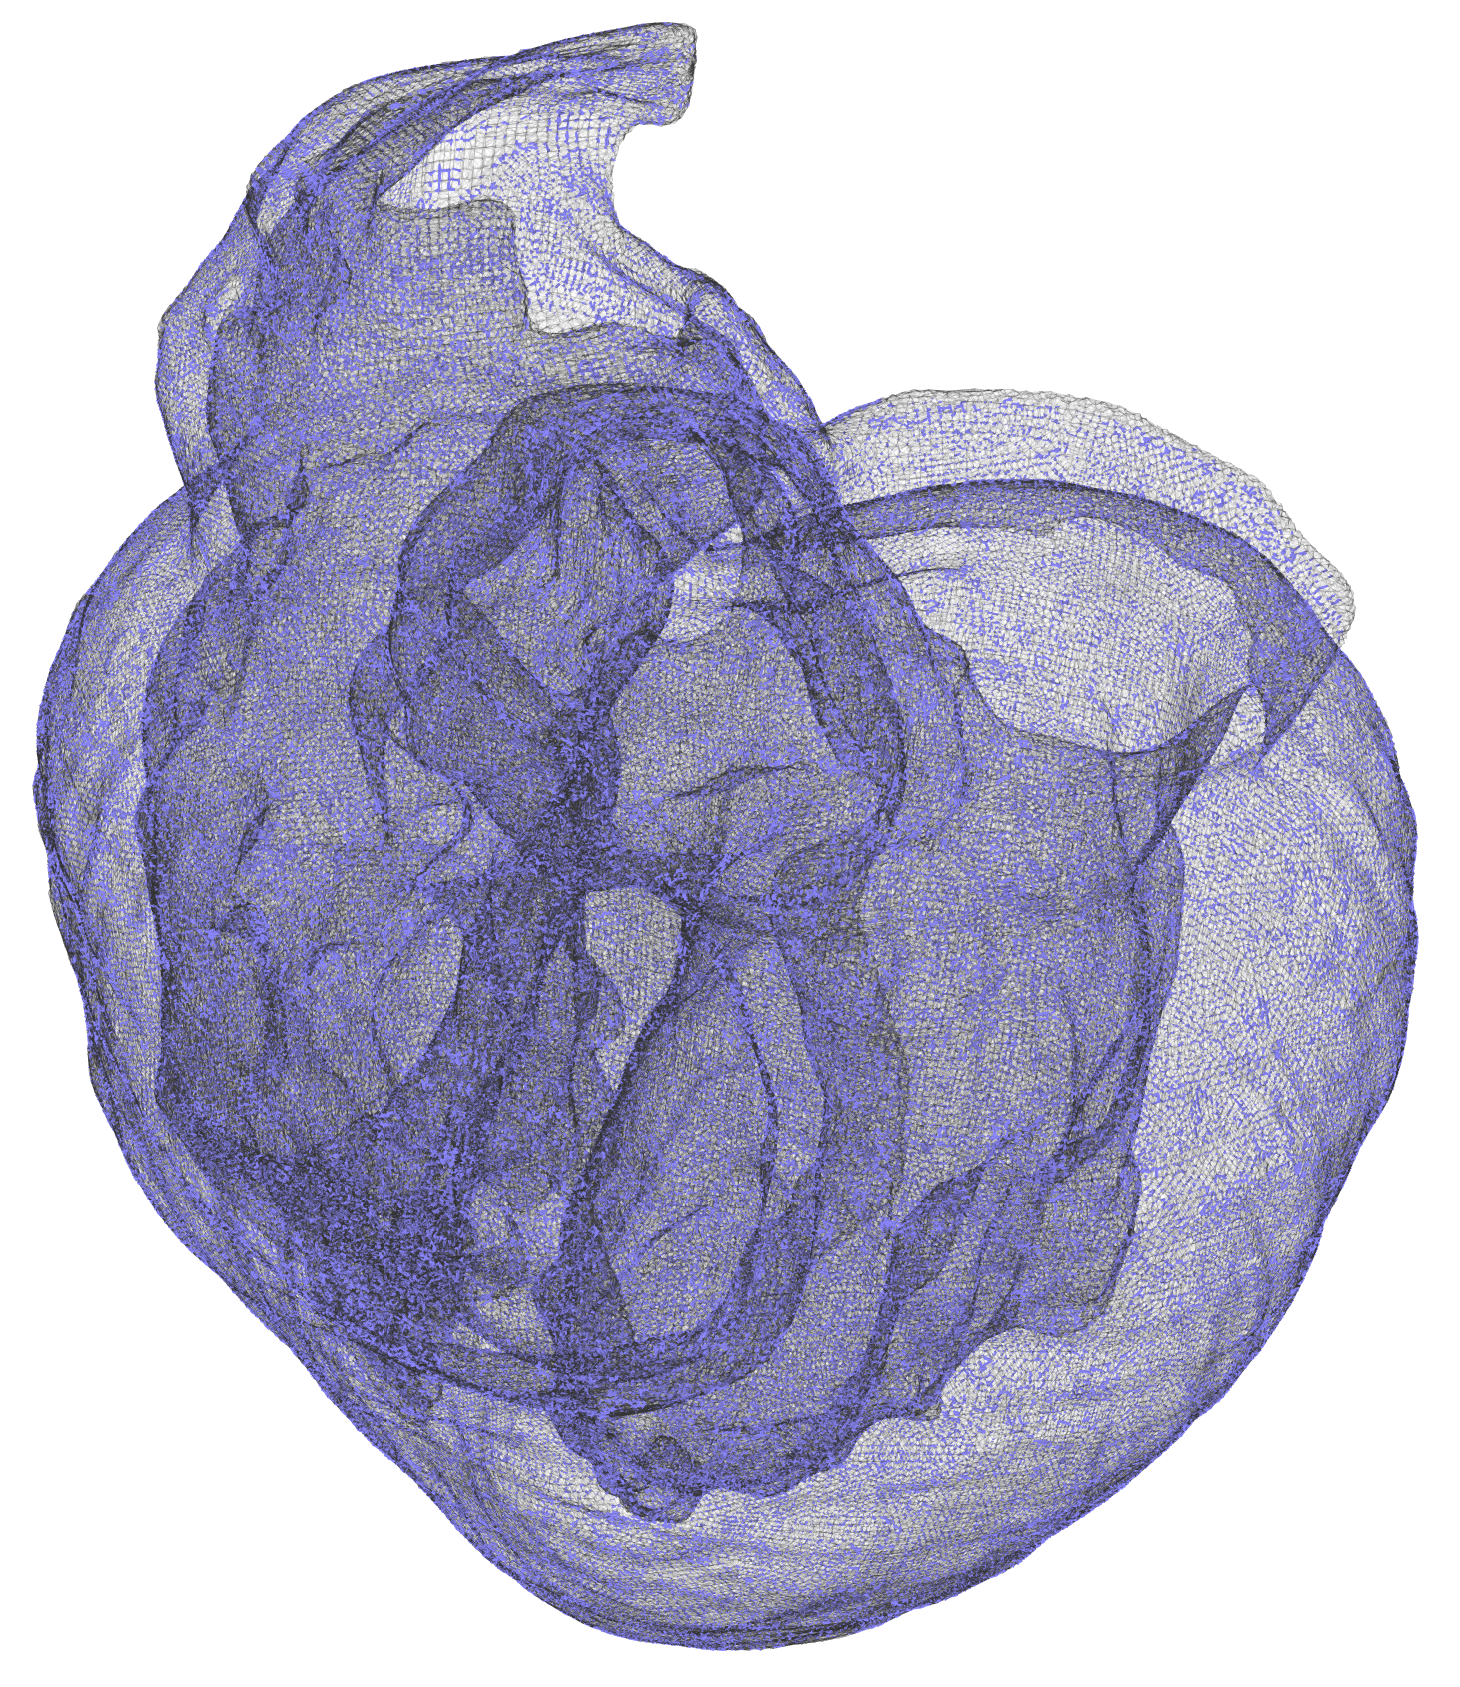
\includegraphics[scale=0.1]{media/2-shabaka/4-clean/3-badsegs.png}	
\label{fig:cross2-3}}						
\subfigure[]{%
		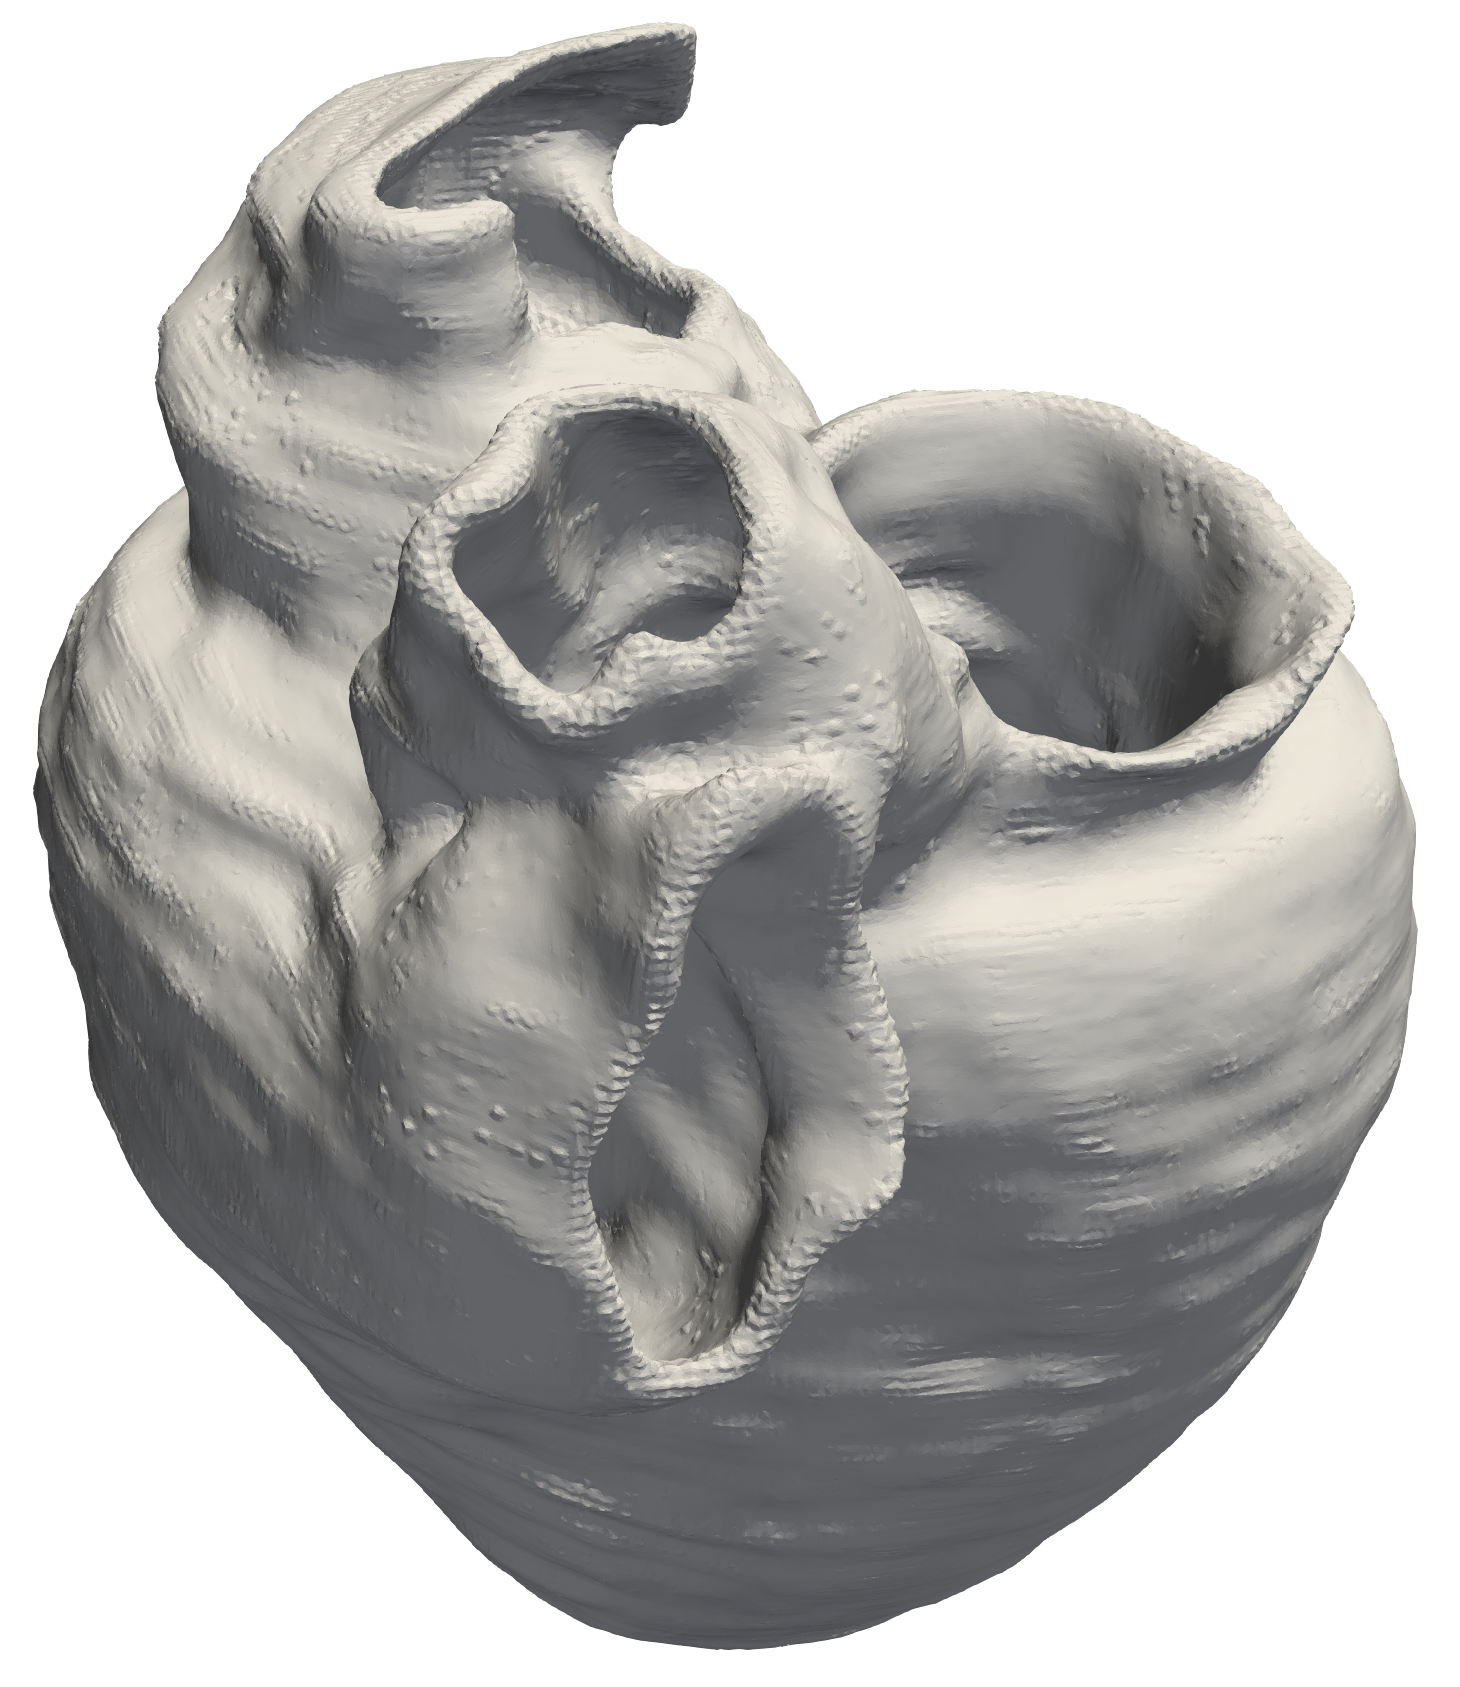
\includegraphics[scale=0.1]{media/2-shabaka/4-clean/4-fine.png}		
\label{fig:cross2-4}}		
%
\caption{Clean-up of undesirable ``cross-talk'' facets for surface of \textit{ex vivo} human heart: (a) initial surface following Voronoi-based surface reconstruction, (b) identification of ``cross-talk'' facets, (c) identification of edges to be collapsed, (d) final cleaned surface}
\label{fig:cross2}
\end{sidewaysfigure}

\subsubsection{Surface Decimation}

Surface \textit{decimation} is performed to reduce the surface mesh to a practical resolution without significantly changing the geometry. The philosophy in image-based meshing, surface extraction, and surface reconstruction is typically to make use of as much information as available to construct a mesh of the highest fidelity possible, and only then to address the practical consideration of mesh resolution for simulation purposes. Indeed, this is what Simpleware's {+FE Free} module does, as described previously. The challenge then becomes decimating in a manner that does not lose more features from the original surface than is desired. For the purposes of this algorithm, decimation is performed using the code \textit{ACVD}~\cite{valette_2004, valette_2008}, which clusters vertices and triangles to generate a coarser surface mesh whose resulting triangles exhibit excellent aspect ratio. The code does not preserve sharp edges or corners, however. This is actually not necessarily an issue for biological structures, as they tend not to have singularities, but would be a problem if the proposed image-based meshing paradigm were extended to meshing mechanical parts from micro-CT scans, for example.

\subsubsection{Results}

Results of the entire surface generation procedure described in this chapter are shown in~\figref{shabakaseq} for the \textit{ex vivo} human heart example. The optimal parameters identified for robust surface generation are shown in~\tabref{Mod5}. The algorithm was rigorously tested with these parameters to produce closed, manifold surfaces for a wide variety of examples. For the \textit{ex vivo} heart, the corresponding point cloud consisted of 236k points, the Voronoi site set comprised of 472k sites, and. the surface mesh prior to decimation yielded 1.00m points and 2.01m triangles. Following decimation, the final surface mesh consisted of 50k points and 100k triangles.

\begin{table}[ht!]
 \centering
   \begin{tabular}{|c||c|c|}
   \hline 
   \textbf{Variable} & \textbf{Description} & \textbf{Value} \\ \hline \hline
   $R_{\mathcal{W}}$ & window radius (in voxels) & 5 \\ \hline
   $d_{\mathcal{W}}$ & sampling distance between adjacent windows (in voxels) & 2 \\ \hline
   \multirow{2}{*}{$\overline{k}_{\mathcal{M}}$ \rule{0mm}{4mm}} & threshold for acceptable ratio of voxels in & \multirow{2}{*}{0.925} \\
   {} & window $\mathcal{W}$ belonging to material $m$ & {} \\ \hline
   $\beta_0$ & functional weighting coefficient for zeroth moment of volume & 0.5 \\ \hline
   $\beta_1$ & functional weighting coefficient for first moment of volume & 0.3 \\ \hline   
   $\varepsilon$ & tolerance for minimization of functional $\mathcal{F}$ & $10^{-14}$ \rule{0mm}{4mm} \\ \hline
   $\overline{\mathcal{F}}$ \rule{0mm}{4mm} & largest acceptable value of functional $\mathcal{F}$ & $0.15$ \\ \hline
   \multirow{2}{*}{$b$} & distance between interface normal and & \multirow{2}{*}{$1.1$} \\
   {} & corresponding Voronoi site pair (in voxels) & {} \\ \hline
\end{tabular}
\caption{Optimal parameter values for b-rep generation}
\label{tab:Mod5}
\end{table}

\begin{sidewaysfigure}[htbp!]
\centering
\subfigure[]{%
		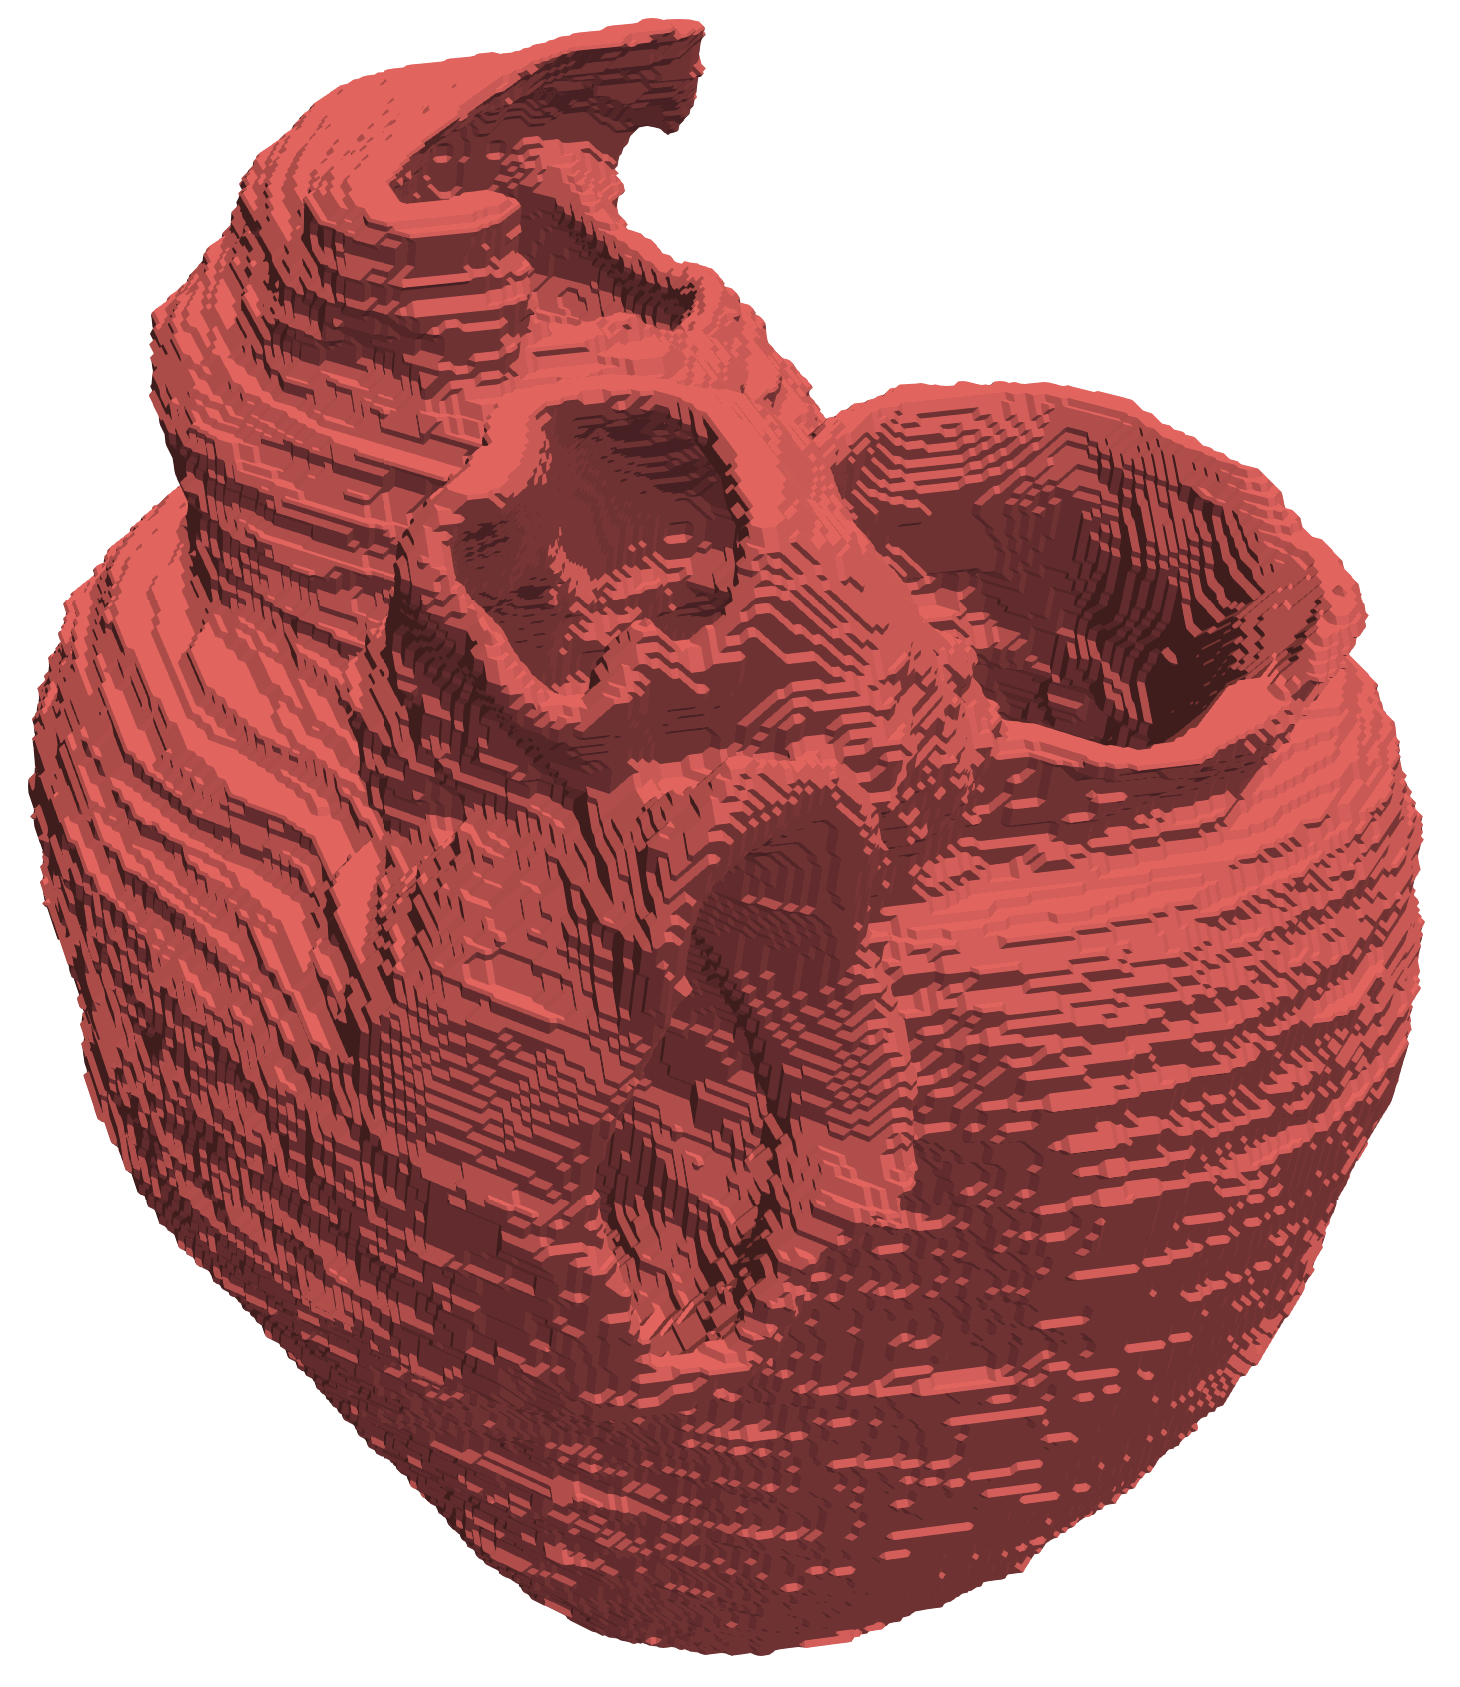
\includegraphics[scale=0.1]{media/2-shabaka/2-surf/1-seg.png}
\label{fig:shabakaseq1}}
\subfigure[]{%
		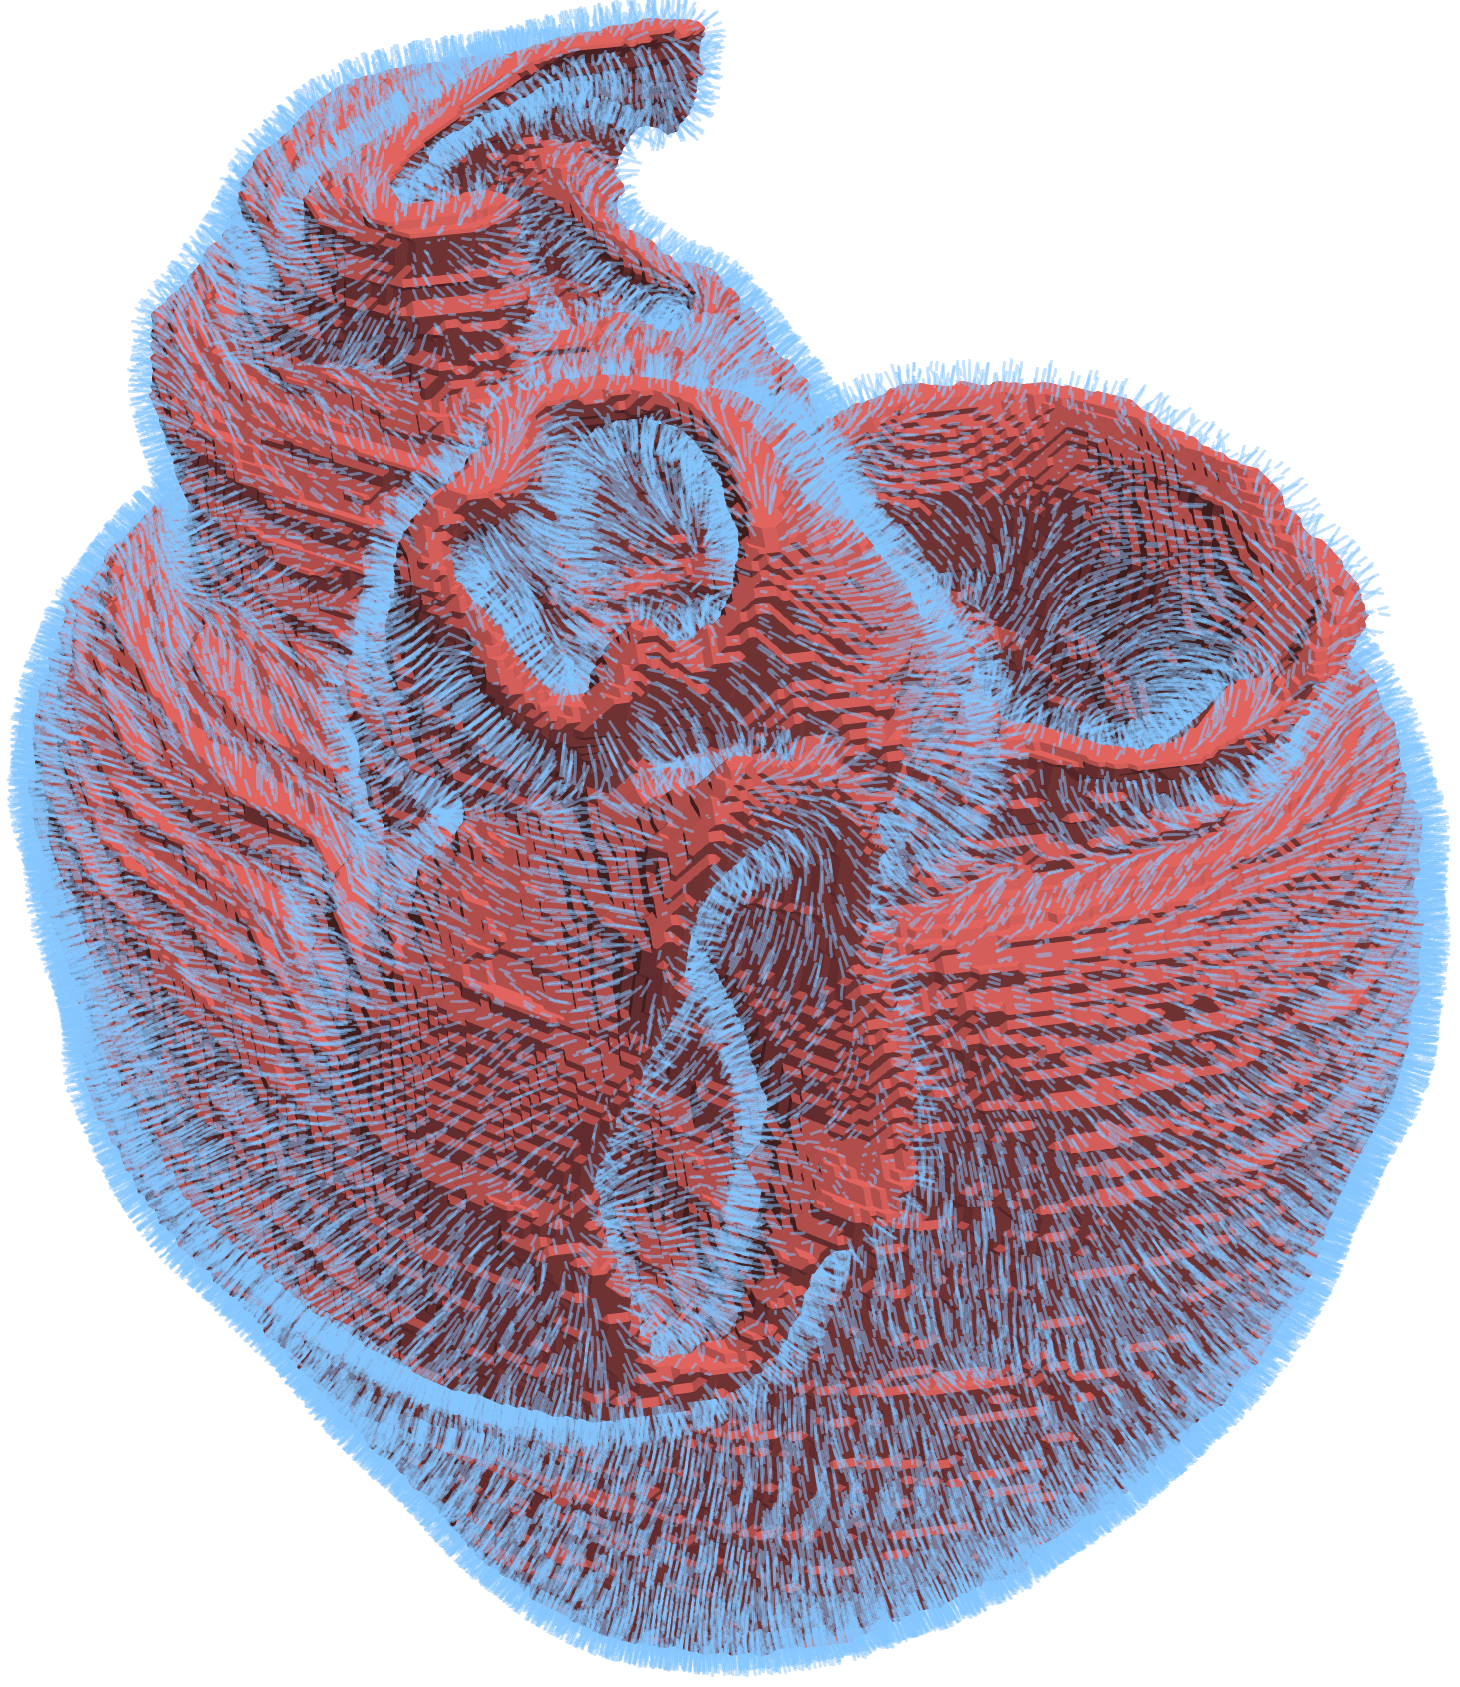
\includegraphics[scale=0.1]{media/2-shabaka/2-surf/2-normals.png}
\label{fig:shabakaseq2}}
\subfigure[]{%
		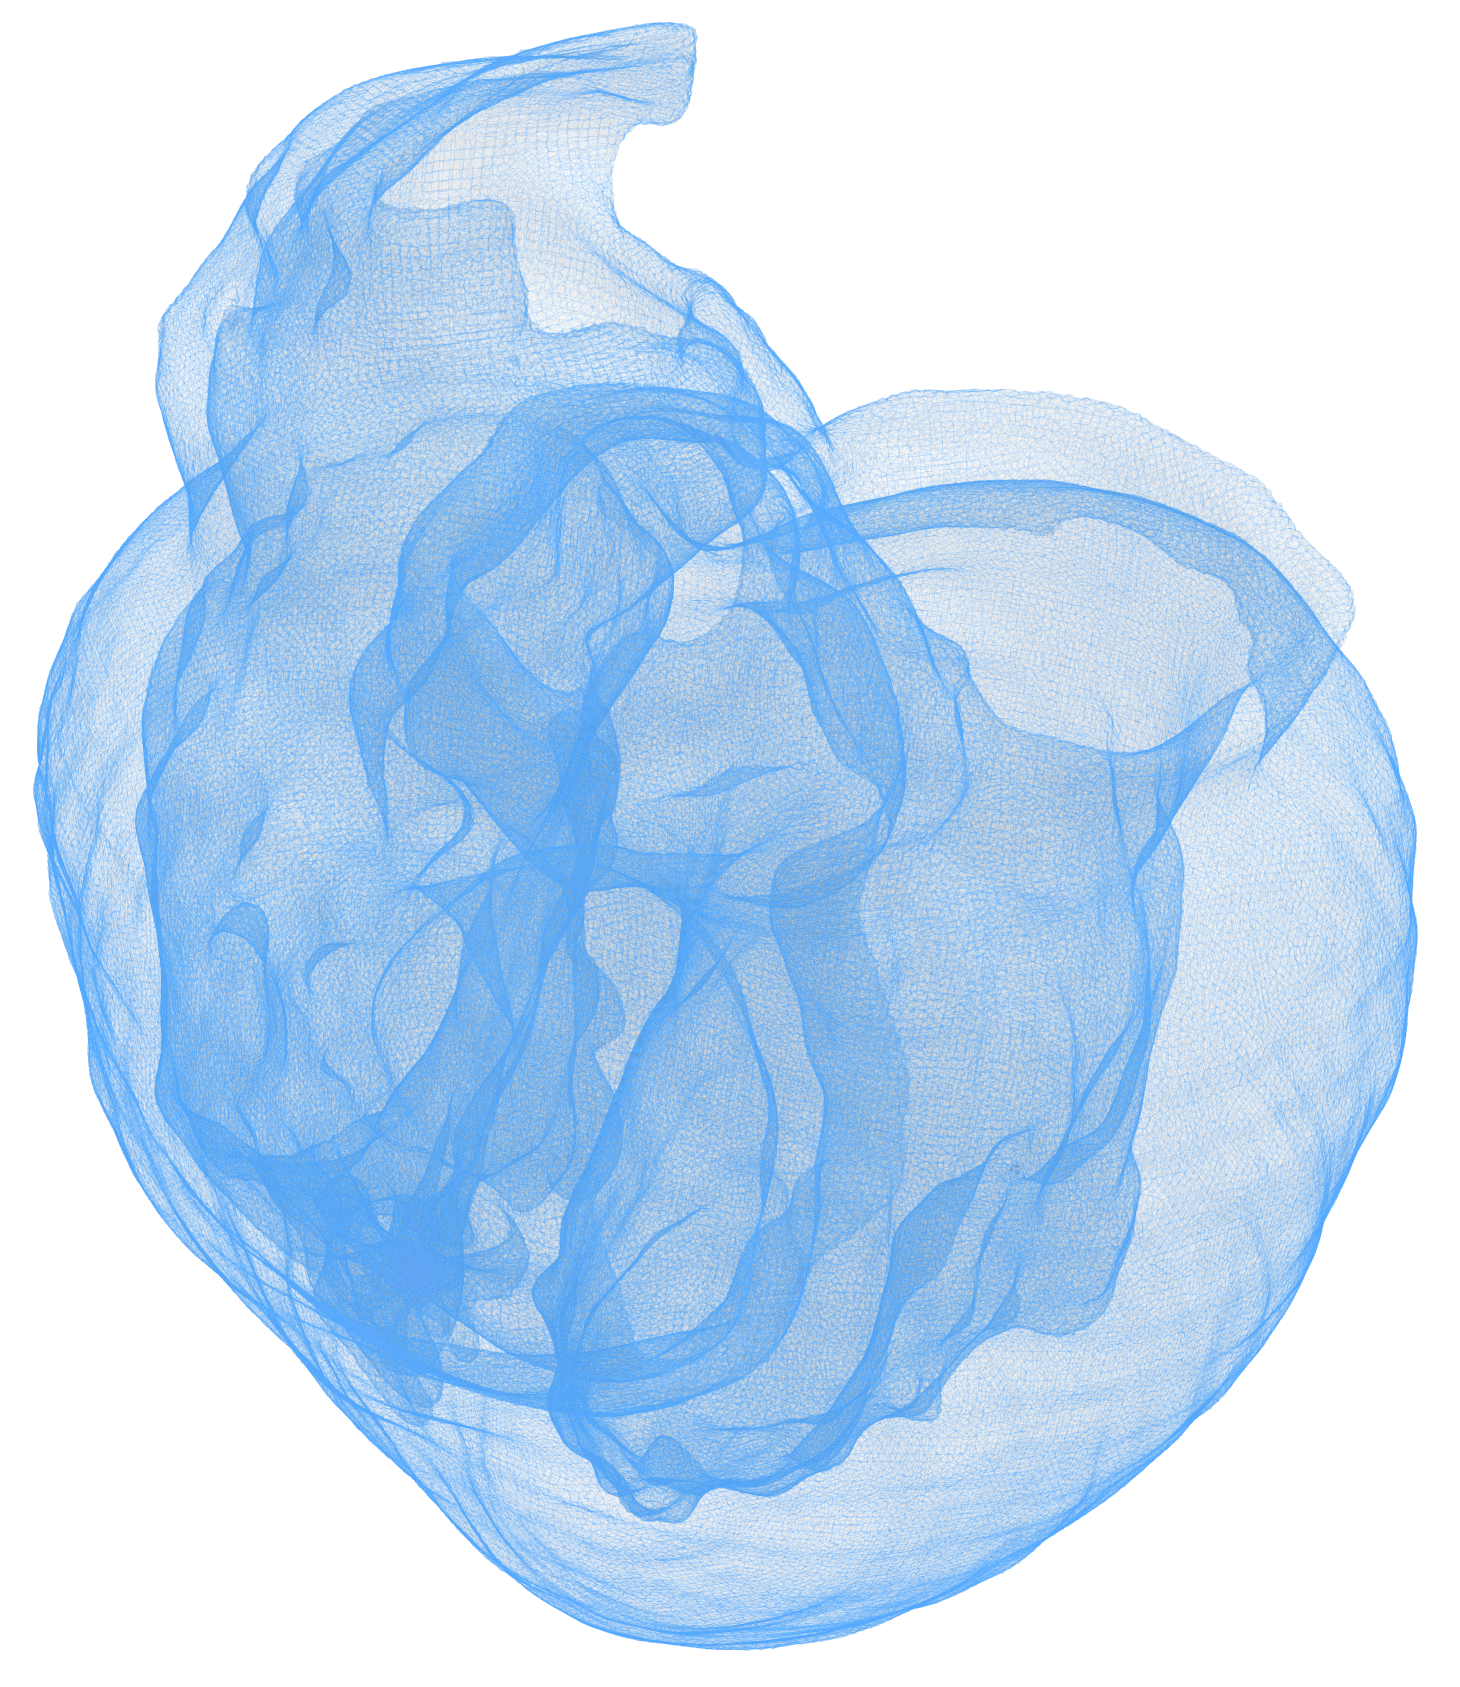
\includegraphics[scale=0.1]{media/2-shabaka/2-surf/3-ptcloud.png}
\label{fig:shabakaseq3}}
\\
\subfigure[]{%
		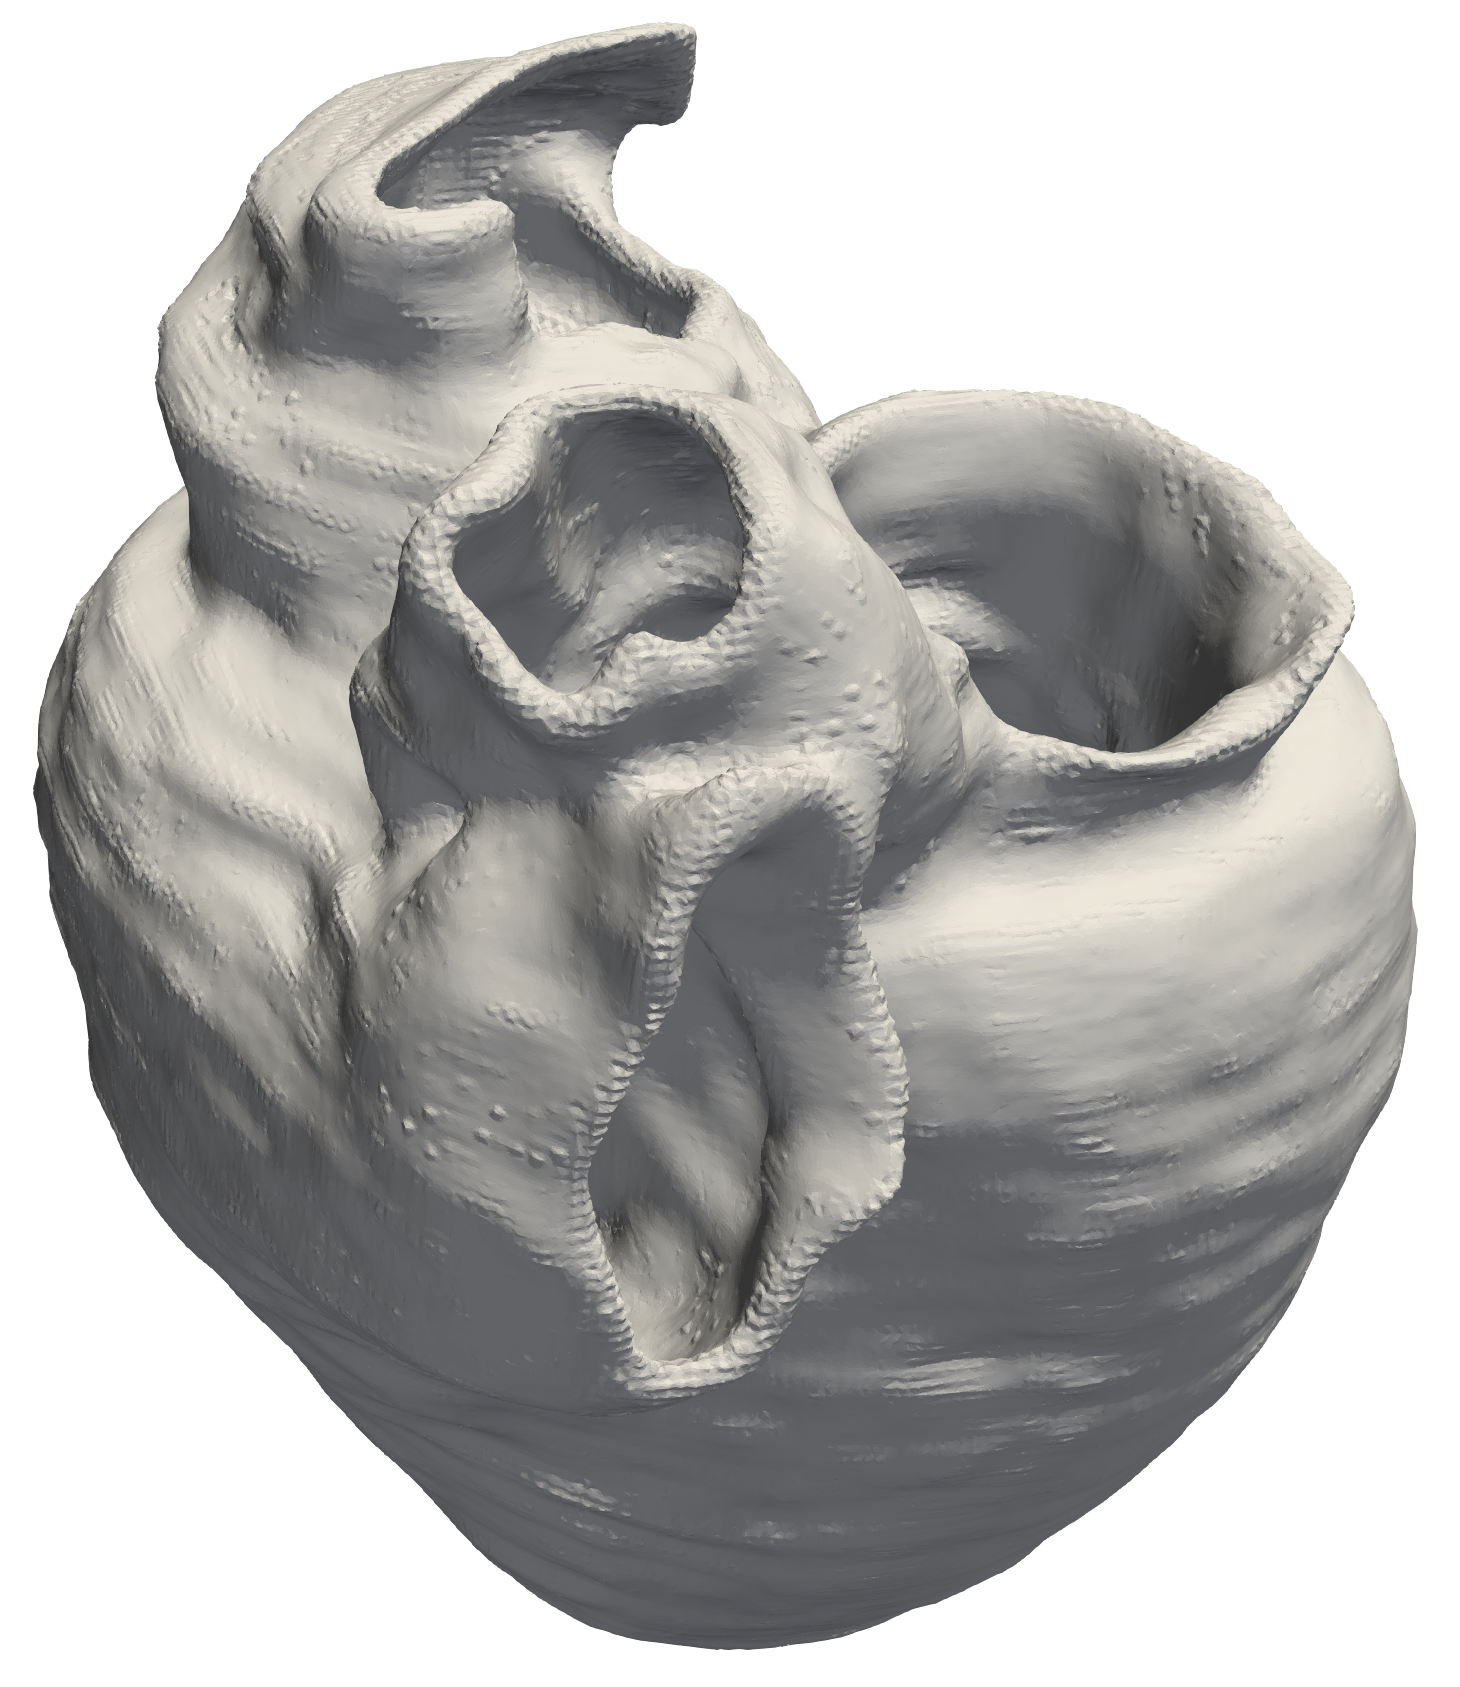
\includegraphics[scale=0.1]{media/2-shabaka/2-surf/4-finesurf.png}
\label{fig:shabakaseq4}}
\subfigure[]{%
		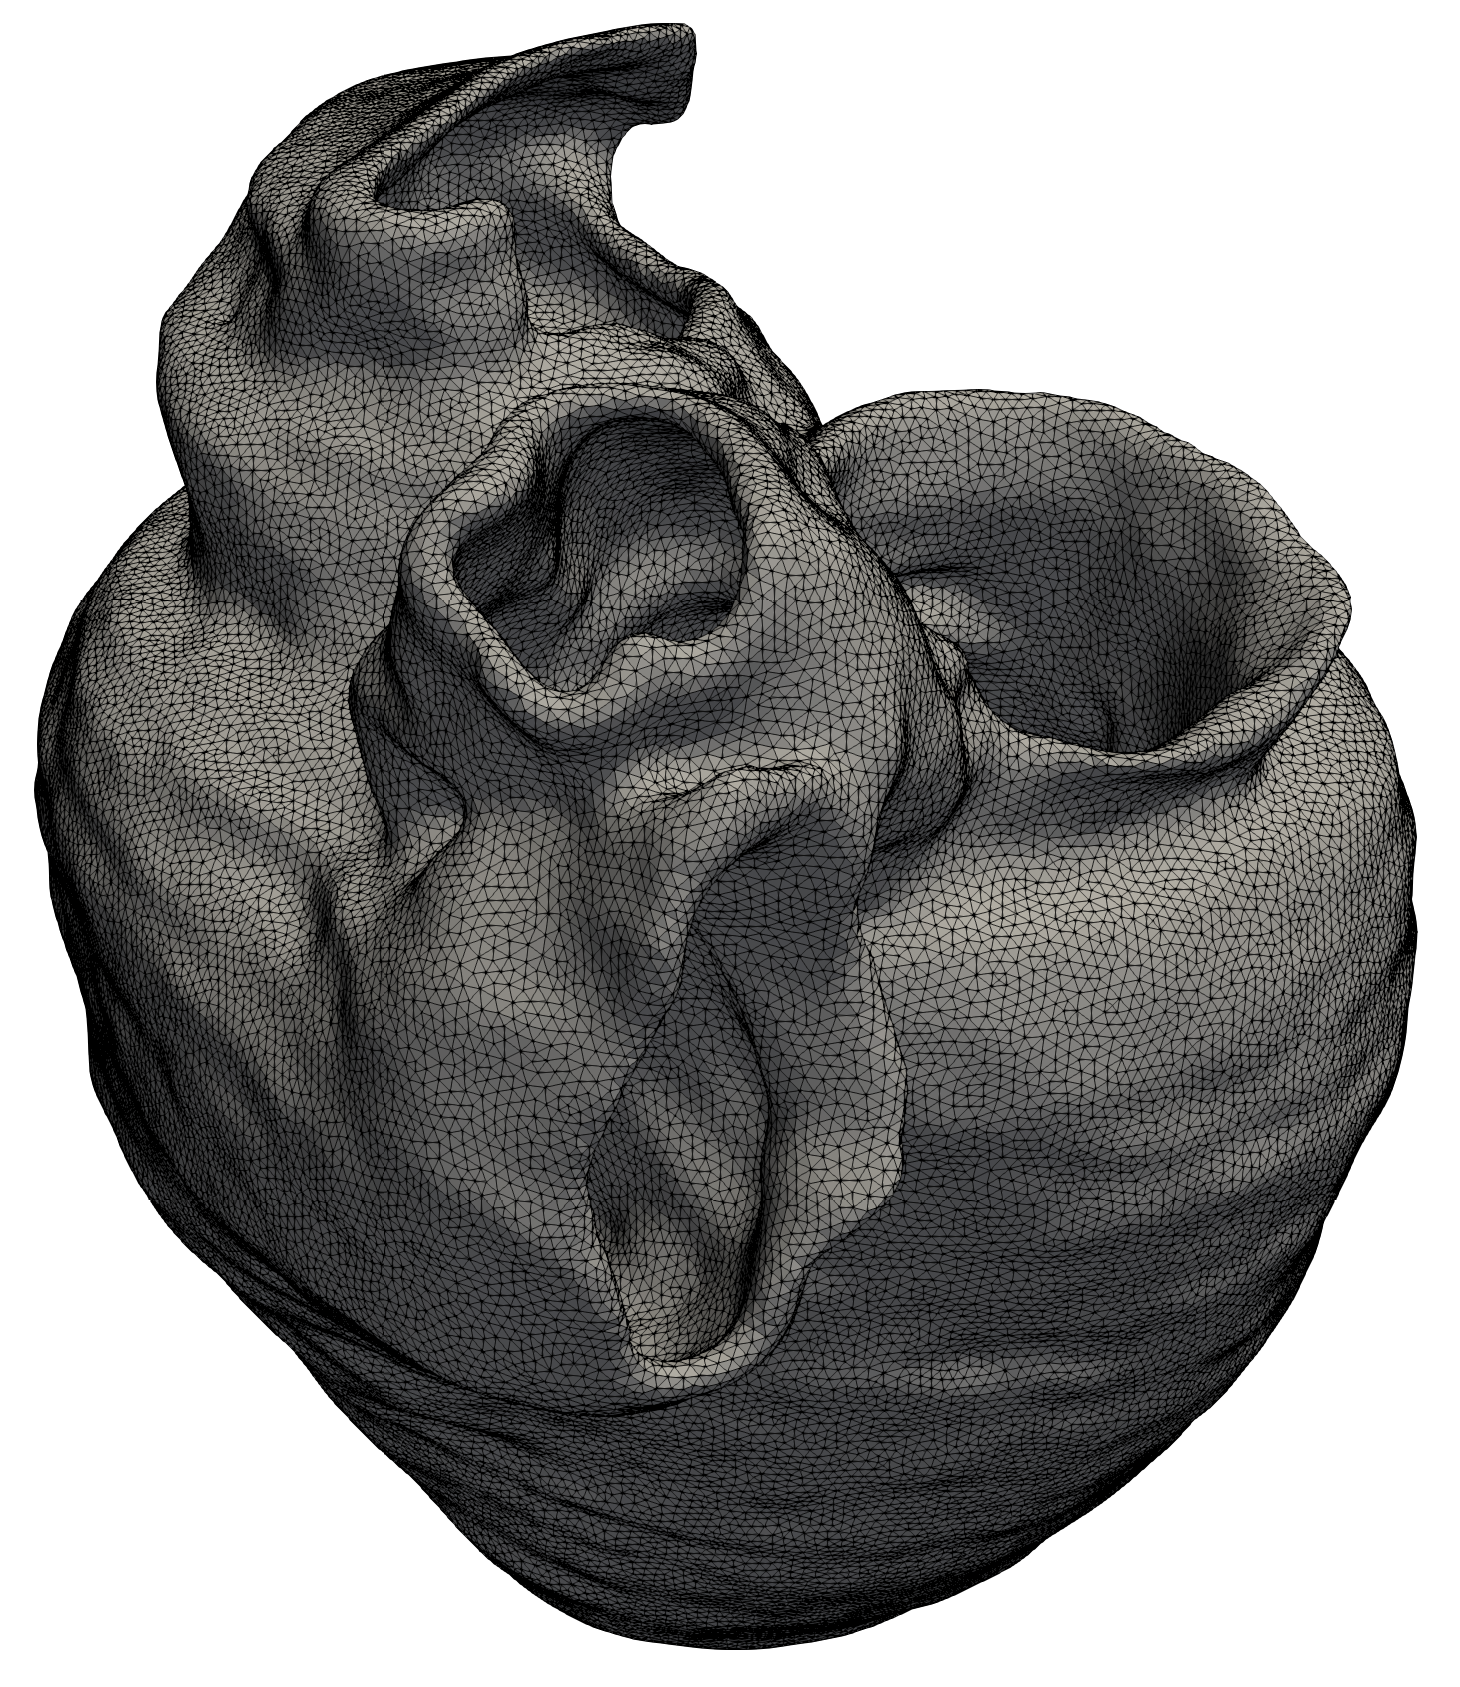
\includegraphics[scale=0.1]{media/2-shabaka/2-surf/5-surf.png}
\label{fig:shabakaseq5}}
%
\caption{(a) Segmented image, (b) point/normal placement, (c) oriented point cloud (normals not shown), c) cleaned surface mesh generated from Voronoi partition (edges not shown), and d) final decimated surface}
\label{fig:shabakaseq}
\end{sidewaysfigure}

%%%%%%%%%%%%%%%%%%%%%%%%%%%%%%%%%%%%%%%%%%%%%%%
%%%%%%%%%%%%%%%%%%%%%%%%%%%%%%%%%%%%%%%%%%%%%%%
\subsection{File Formats}
\label{File Formats-SURF}

Among free software, the simplest and most prevalent file formats for storing point clouds and surface meshes are the Stanford Polygon Format (PLY)~\cite{ply} and the Visualization Toolkit Format (VTK)~\cite{vtk}. Similar to the file format of images and image masks, these formats include a header that describes the data that it precedes. The number of vertices is included in the header, as well as a list of expected point data in the file (e.g., spatial coordinates, normal components). Both file formats handle many different data types (again, \texttt{unsigned char}, \texttt{int}, etc.), so the data type of each piece of data must be prescribed as well. The data itself simply includes vertex coordinates, additional vertex property data if available, and in the case of meshes, the vertex connectivity of facets.

Once again, the raw data may be stored in ASCII or binary format. ASCII format for these point clouds and surface meshes holds significantly more value for these data types than for images or image masks, as specific vertex coordinates and/or connectivities can be queried or even modified. However, for dense point clouds or fine meshes, file sizes can become intractable, and thus binary storage is still the preferred route. Newer editions of the VTK format store data in XML format but were not explored for the purposes of this work.

The Stereolithography (STL) file format is, unfortunately, still the most popular manner in which surface meshes are stored. STL files store a list of independently defined triangles based on vertex coordinates. Thus, for a closed surface the amount of unnecessarily repeated vertex coordinate data can balloon. The tolerances for which the STL file is generated and subsequently read can cause much more serious problems though. For example, if the tolerance for which the STL is generated is less than that for which it is read (potentially in a different piece of software), the file may be incorrectly deemed non-manifold, and require processing to address the problem. This of course is a non-issue for file formats like PLY and VTK, in which vertices are explicitly defined and numbered in the file, rather than requiring the software reading the file to determine that information.

\section{Mesh Generation}
%
Provided an appropriate surface mesh, CAD-based meshing techniques seek to automatically generate an unstructured discretization of the enclosed volume. Under rare circumstances, the topology of the object of interest may allow for a \textit{structured} mesh, in which there is a predictable repeated connectivity among neighboring elements. To accommodate a surface of arbitrary form, though, an \textit{unstructured} mesh is necessary. The challenge in automated meshing is to maximize the element shape quality while minimizing computational cost or human intervention~\cite{blacker_2001}. The discussion will focus on generating meshes for simulations using finite element methods and its variants. For conventional finite element approaches, topological restrictions on the mesh elements make tetrahedral and hexahedral shapes the most popular choices. Hex and tet meshing approaches have had some success, but not without serious drawbacks. Polyhedral meshing is considered as an alternative, to be used in conjunction with polyhedral finite element methods. Established meshing techniques are summarized, together with a demonstration of the advantages of the polyhedral approach.

%%%%%%%%%%%%%%%%%%%%%%%%%%%%%%%%%%%%%%%%%%%%%%%
%%%%%%%%%%%%%%%%%%%%%%%%%%%%%%%%%%%%%%%%%%%%%%%
\subsection{Hexahedral Meshing}
\label{Hexahedral Meshing}

In general, hexahedral meshes produce the most accurate solutions in finite element simulations and are more computationally efficient than its alternatives~\cite{tautges_2001}. Additionally, for problems involving near-incompressibility, mitigation strategies for volumetric locking like \textit{F-bar projection} are more developed and tested for linear 8-node hexes compared to, say, higher order tetrahedra. To date, though, no algorithm exists that can perform automatic hexahedral meshing of surfaces with arbitrary geometry and topology. The difficulty lies in the strict nodal connectivity constraints that require the hexahedral discretization to consist of either stacks of elements or closed loops~\cite{young_2008}. 

Among the most popular classes of hexahedral meshing techniques are: \textit{primitives}, \textit{overlay grid}, and \textit{automated decomposition}~\cite{blacker_2001}. \textit{Primitives} typically involve producing a 2D unstructured quad mesh of a cross section, followed by \textit{sweeping} the constant topology cross section. This approach is limited to topologies involving a swept cross-section. \textit{Overlay grids} produce a structured background grid and then cut elements and/or modify vertices so that the hex elements near the surface conform to the original surface.  However, this approach can lead to elements with potentially very poor quality. \textit{Automated decomposition} techniques attempt to decompose the volume into separate parts that are subsequently meshed based on swept volumes or other primitive shapes. Decomposing the surface typically requires some degree of manual guidance, though. These approaches suffer from difficulty in matching meshes at part interfaces, and they require potentially significant user-driven de-featuring of the surface.

Hexahedral meshing algorithms typically only apply to a limited set of geometries. In practice, human intervention is necessary to decompose the geometry according to the algorithms available, adjust the geometry as needed to accommodate those algorithms, and - much like image segmentation - potentially select between a suite of tools to be employed as needed~\cite{blacker_2001}. These manual efforts can become impracticably time consuming or even impossible for surfaces of biological tissues, and thus fully hex meshes are not typically used in biomechanics applications.

Mixed element approaches attempt to alleviate the difficulty of producing fully hexahedral meshes by only requiring the mesh to be \textit{hex dominant}. In hex dominant meshes, tetrahedra exist where a hexahedral mesh is intractable, and pyramid elements are required in the transitional layers between hexes and tets. These techniques tend to either: convert an already existing tetrahedral mesh to a hex-dominant mesh by combining tetrahedral elements~\cite{baudouin_2014, gao_2017}; attempt to honor the surface with tetrahedral elements together with an octree hexahedral representation in the interior of the volume~\cite{young_2008, lobos_2015}; or insert tetrahedral elements toward the interior of the volume where frontal approaches of purely hex meshes fail~\cite{blacker_2001}. These approaches have shown promise in meshing arbitrary domains, but little work has been done in evaluating the accuracy and performance in a finite element setting in comparison to fully hex or fully tet meshes~\cite{tautges_2001}.

%%%%%%%%%%%%%%%%%%%%%%%%%%%%%%%%%%%%%%%%%%%%%%%
%%%%%%%%%%%%%%%%%%%%%%%%%%%%%%%%%%%%%%%%%%%%%%%
\subsection{Tetrahedral Meshing}
\label{Tetrahedral Meshing}

The two most widely adopted approaches for automated unstructured tetrahedral mesh generation are \textit{advancing front} and \textit{Delaunay tetrahedralization}~\cite{lohner_1997}. In advancing front techniques~\cite{jin_1993, lohner_1988}, elements are inserted one at a time, starting from the initial triangular surface mesh and working toward the interior of the enclosed volume. Care must be taken to avoid poor element quality when the front collides from different directions. The success of the approach depends on the initial quality and size of the triangular surface mesh, which can be remedied by surface remeshing/decimation.

Delaunay tetrahedralization is the dual of the previously described \textit{Voronoi diagram}. Namely, the Voronoi sites form the vertices of the Delaunay tetrahedralization, whose edges perpendicularly pass through the corresponding shared Voronoi facets. The set of tetrahedra satisfy the property that no other vertex is contained within the circumsphere formed by the vertices of each tetrahedron. The Delaunay tetrahedralization is typically constructed incrementally. A tetrahedralization is carried out on an initial point distribution. Additional points are introduced and tetrahedra encompassing the new point are removed. The void created by the deletion of these tetrahedra is then remeshed~\cite{young_2008}. The specification of the initial point distribution and subsequent insertion of points dictates the resulting quality of the mesh elements. Constraining the Delaunay tetrahedralization to adhere to the input surface can also severely affect element quality and even produce sliver elements~\cite{lohner_1997}.

A Delaunay meshing implementation from \textit{Tetgen}~\cite{tetgen} is utilized to generate high-quality tetrahedral meshes of linear or quadratic order that exactly honor input surface meshes. A tetrahedral mesh of the ventricles of the \textit{ex vivo} heart example is shown in \figref{tetmesh}.

\begin{sidewaysfigure}[htbp!]
\centering
\subfigure[]{%
		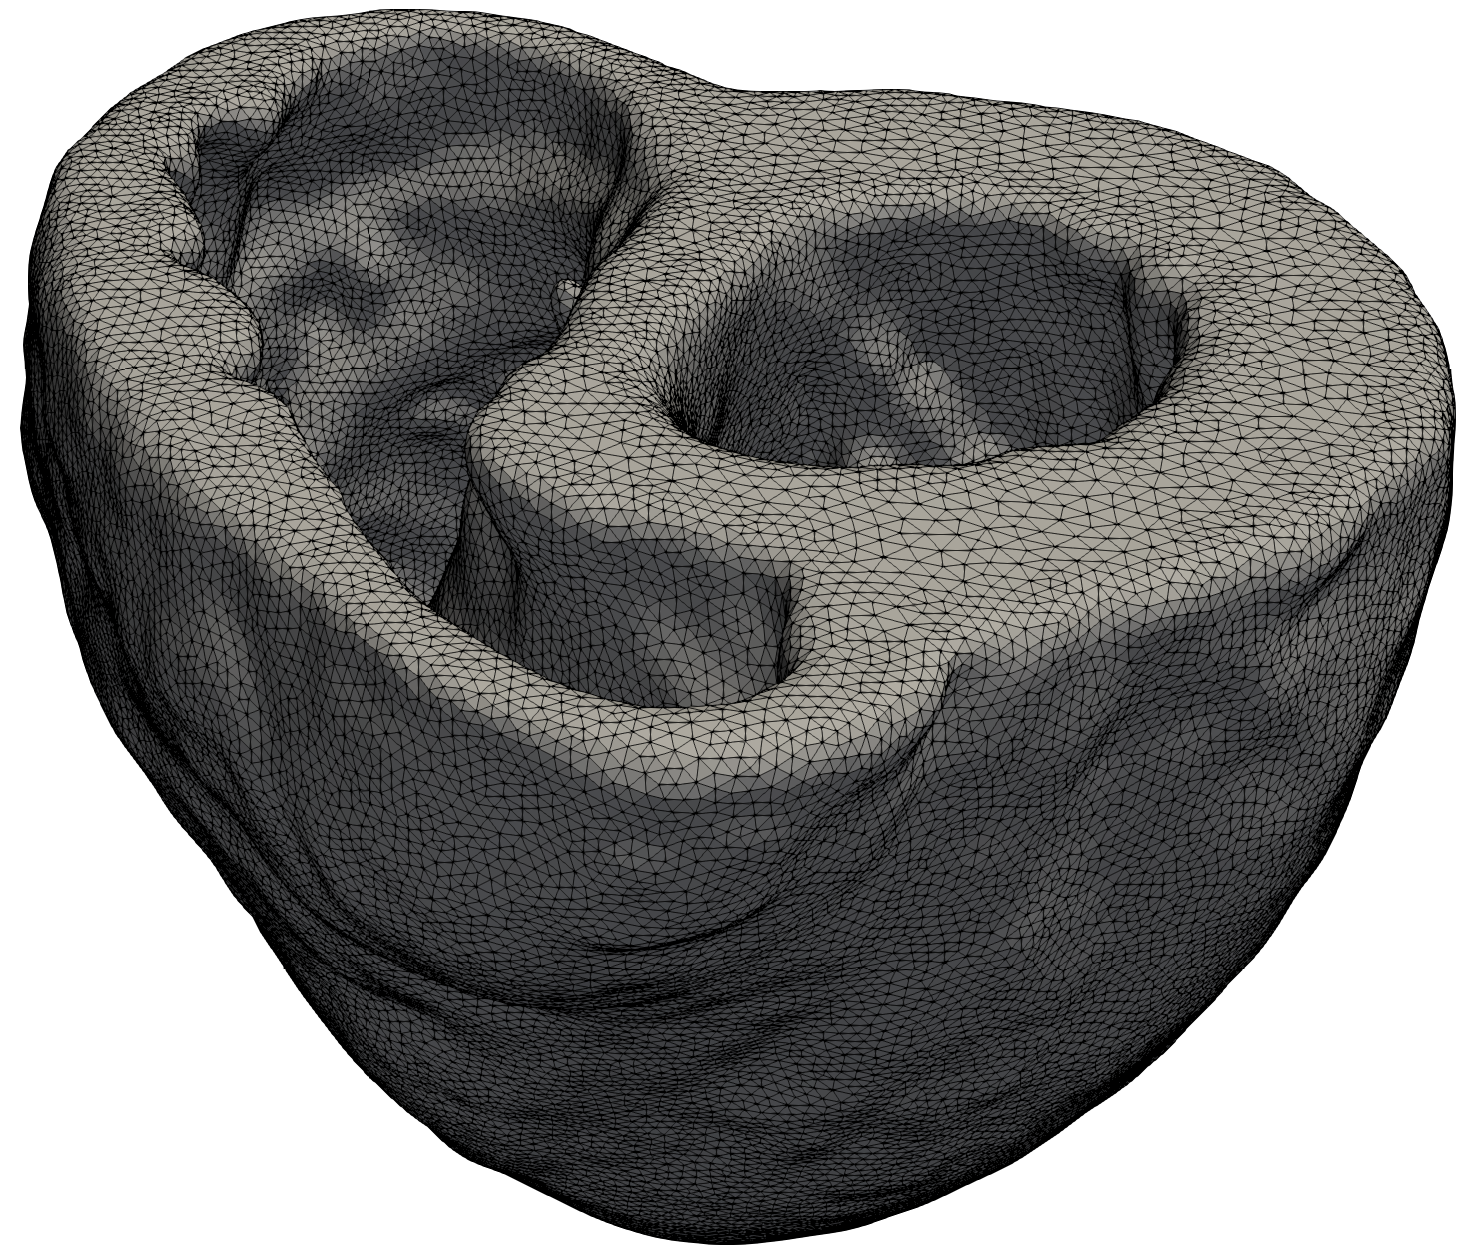
\includegraphics[scale=0.16]{media/4-cardioid/0-ventriclesurf.png}
\label{fig:tet1}}
\subfigure[]{%
		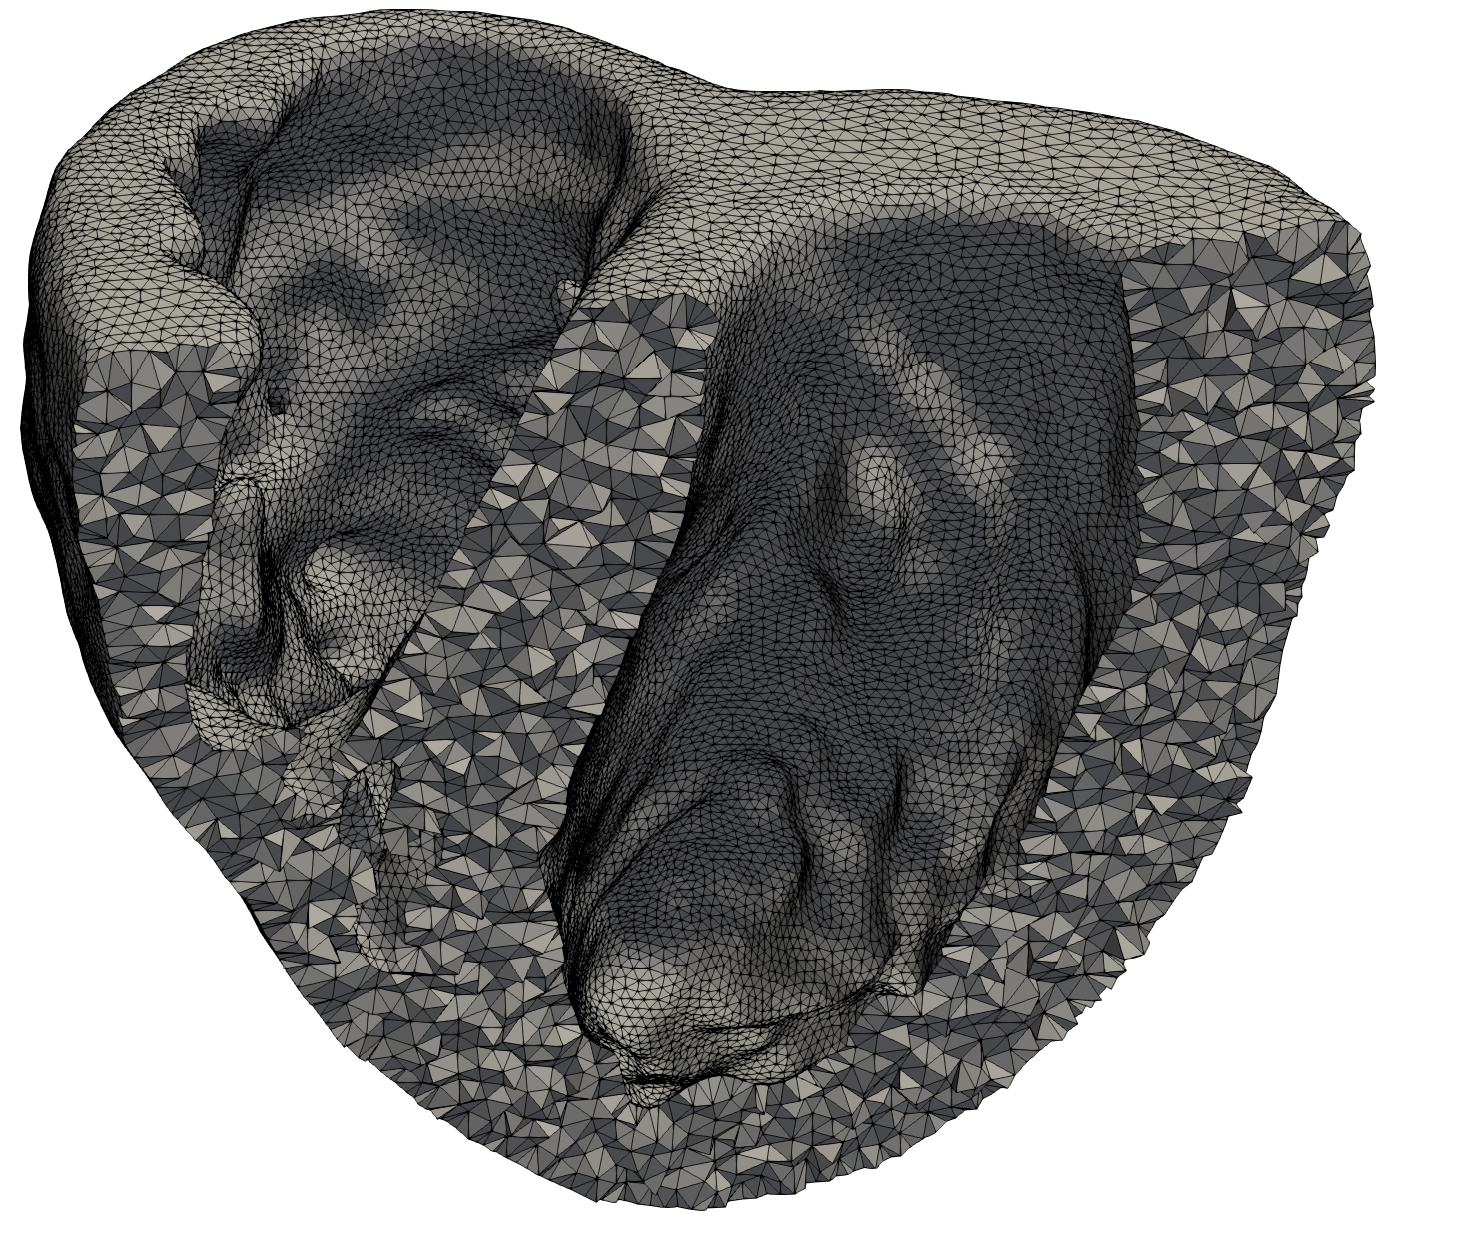
\includegraphics[scale=0.16]{media/4-cardioid/1-tet.png}
\label{fig:tet2}}
%
\caption{Bi-ventricular mesh of \textit{ex vivo} human heart: (a) input surface mesh, and (b) clipped view of quadratic tetrahedral mesh}
\label{fig:tetmesh}
\end{sidewaysfigure}

%%%%%%%%%%%%%%%%%%%%%%%%%%%%%%%%%%%%%%%%%%%%%%%
%%%%%%%%%%%%%%%%%%%%%%%%%%%%%%%%%%%%%%%%%%%%%%%
\subsection{Polyhedral Meshing}
\label{Polyhedral Meshing}

Although hexahedral meshes are generally preferred for conventional finite element approaches, to date there are no techniques available that offer a robust automatic pipeline to generate hex meshes. Thus, tetrahedral mesh generation tools are typically the de facto choice for image-based meshing. Linear tet elements can only represent a constant strain, however, leading to inaccurate solution approximation unless impractically fine meshes are used. Generally speaking, linear tets are not to be used for nonlinear solid mechanics problems involving near-incompressibility~\cite{hughes_2000}, tension, torsion, bending~\cite{wang_2004, benzley_1995}, or contact~\cite{maas_2016}. Quadratic tets, on the other hand, produce much more accurate results and are generally the most popular element choice for biological applications. For problems involving complex geometries and/or requiring high fidelity solutions, though, the resulting problem size for quadratic tet meshes can be problematic. Polyhedral meshes, in conjunction with polyhedral finite element methods, attempt to compete with the robustness of tetrahedral meshes and the accuracy and computational efficiency enjoyed when using hexahedral meshes.

Polyhedral meshing approaches tend to fall under two categories: those that seek to produce a Voronoi partition of the domain, and those that seek a hex-dominant mesh. Meshing techniques that seek to generate Voronoi partitions~\cite{garimella_2014, lee_2015} offer the advantage of exclusively convex elements with desirable aspect ratios. However, this comes at the price of needing to remesh the surface, which re-opens the issue of feature preservation. Indeed, Ebeida \textit{et al.}~\cite{ebeida_2011, mitchell_2015} for example, strategically sampled the input surface mesh before reconstructing it. Special care must be taken to sample regions of high curvature and sharp corners, and these features are not well preserved for some of the examples shown in their work. Additionally, for more general CAD-based meshing applications, it may be desirable to preserve the input surface mesh even if all features are honored exactly, for the purposes of applying boundary conditions or mating adjacent parts later.

Hex-dominant polyhedral meshing ``sculpts'' a background hex mesh with the input b-rep, producing hexahedra on the interior and arbitrary polyhedral shapes near the surface. These arbitrary polyhedra are accommodated by an element formulation that deviates from the conventional FEM approach, to be discussed in~\chapref{4}. This sculpting approach must handle geometric near-degeneracies in a robust way. Indeed, topological correctness is the highest priority if one is to guarantee a simulation-ready mesh for an arbitrary input surface. An implementation of such an approach in the polyhedral FEM software \textit{Celeris} is used to generate polyhedral meshes from input b-reps~\cite{rashid_2013}. To avoid undesirably small elements, the intersection calculation between the input b-rep and its corresponding bounding hex mesh is tolerance-driven. Each polytope of the b-rep and bounding hex mesh is stored via a recursive definition of lower dimensional polytopes, and thus intersections are calculated in stages from lower order polytopes to higher order. In this manner, intersections of dimension greater than zero only require integer logic, and floating-point calculations are kept to a minimum~\cite{rashid_2013}. \figref{cel} illustrates the robust polyhedral meshing sequence, and~\figref{zoom} shows some example arbitrary polyhedral elements for which a novel element formulation is required.

\begin{sidewaysfigure}[htbp!]
\centering
\subfigure[]{%
		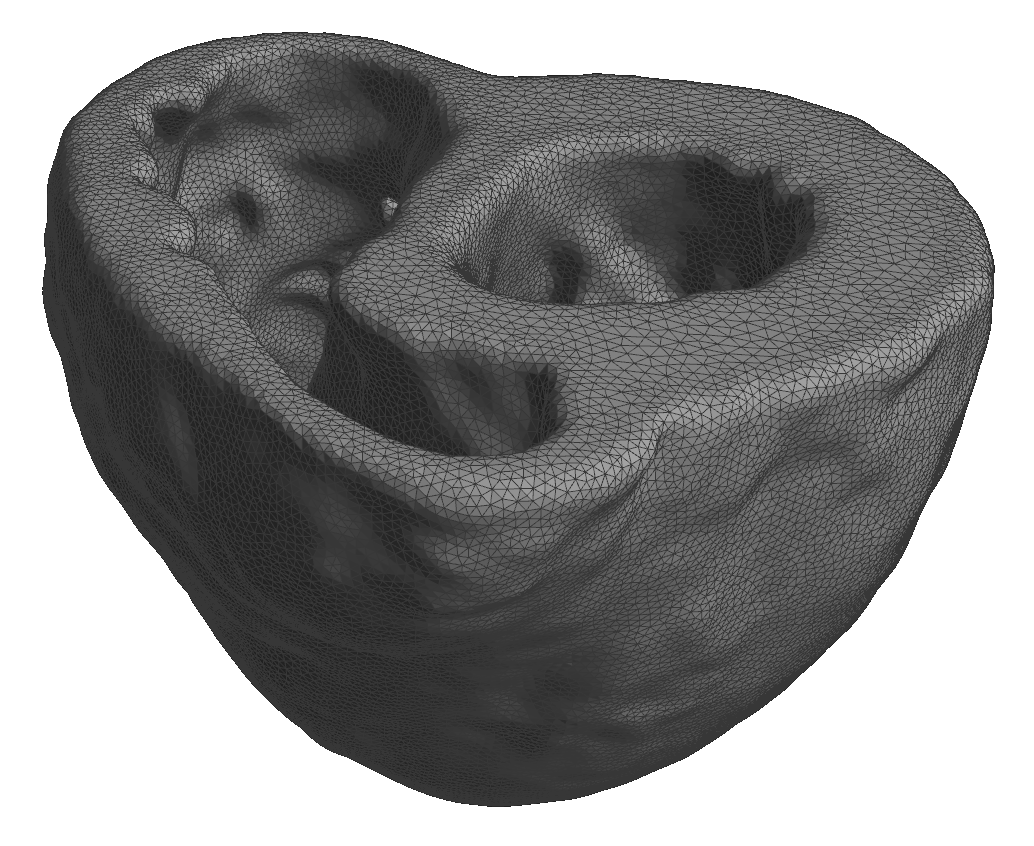
\includegraphics[scale=0.18]{media/3-celeris/1-brep.png}
\label{fig:cel1}}		
\subfigure[]{%
		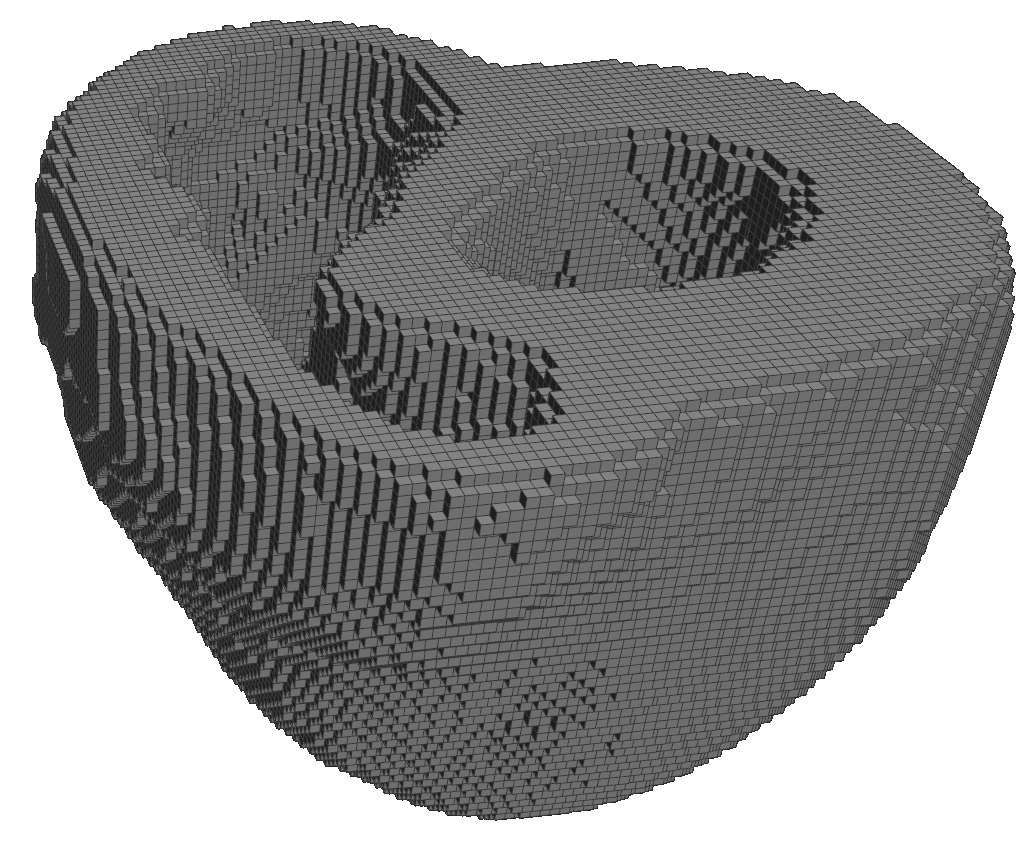
\includegraphics[scale=0.18]{media/3-celeris/2-hex.png}
\label{fig:cel2}}		
\subfigure[]{%
		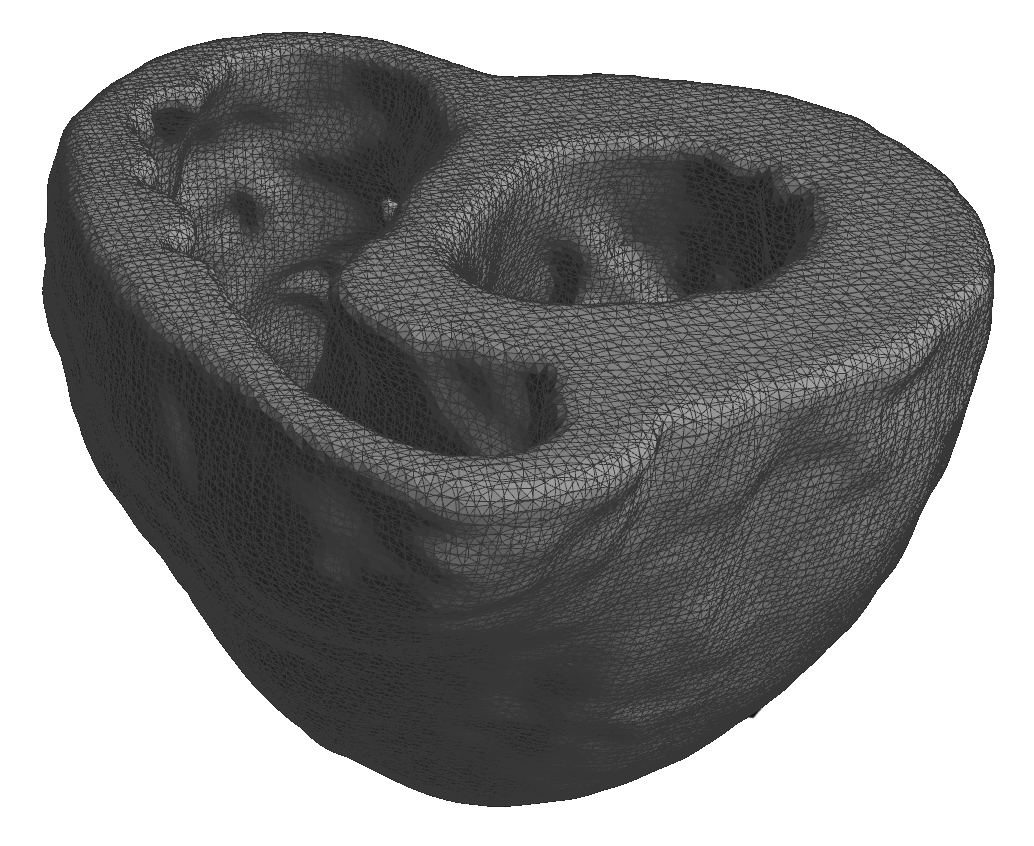
\includegraphics[scale=0.18]{media/3-celeris/3-pmesh.png}
\label{fig:cel3}}
\\		
\subfigure[]{%
		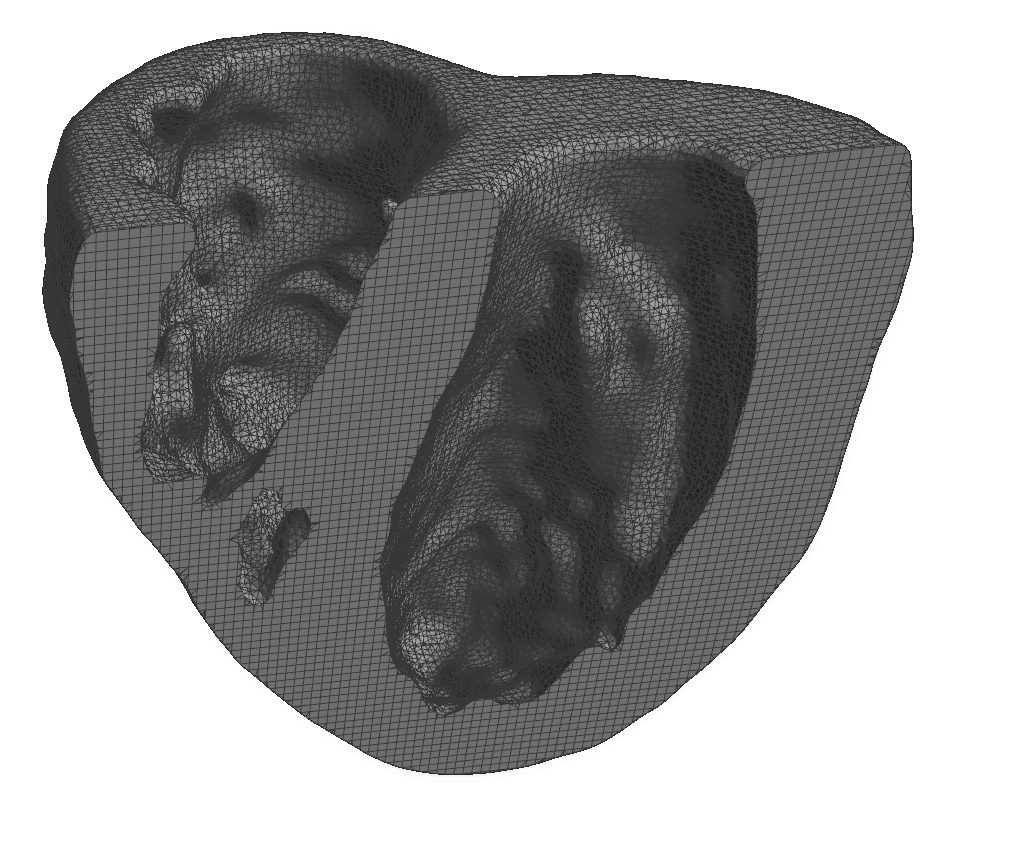
\includegraphics[scale=0.18]{media/3-celeris/4-clip.png}
\label{fig:cel4}}	
\subfigure[]{%
		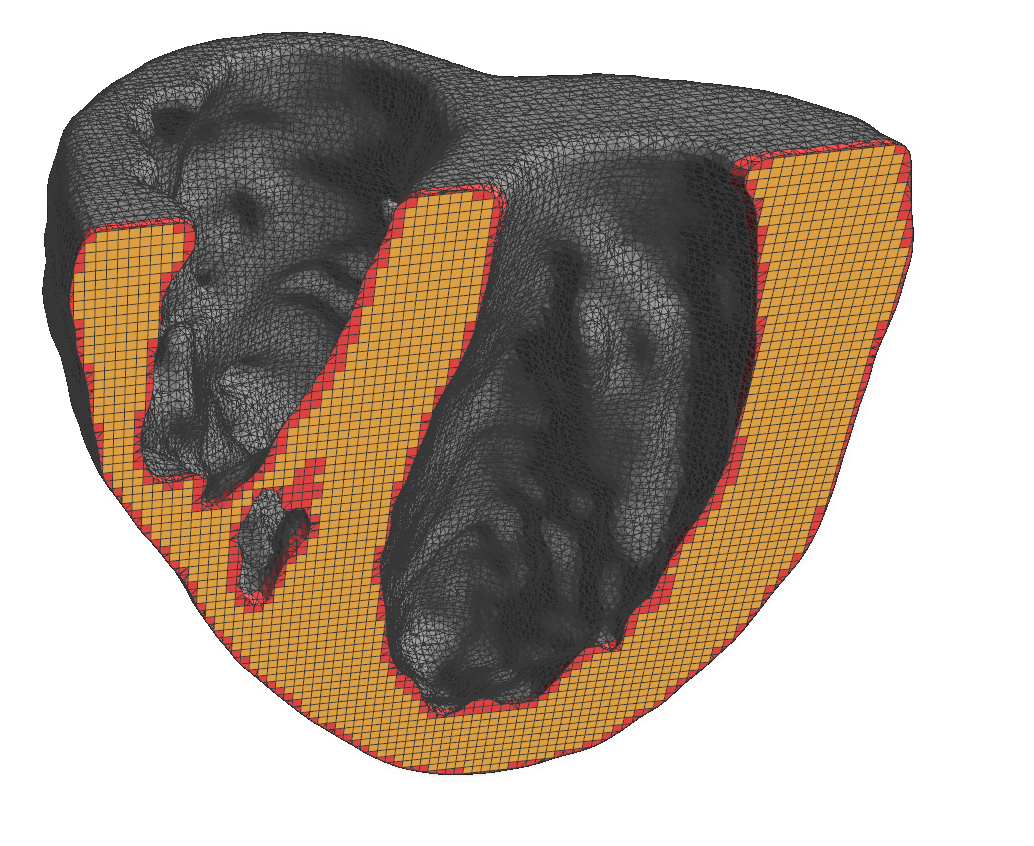
\includegraphics[scale=0.18]{media/3-celeris/5-color.png}
\label{fig:cel5}}			
\caption{Generation of polyhedral mesh: (a) input surface mesh, (b) bounding hex mesh,  (c) resulting polyhedral mesh, (d) clipped mesh, and (e) highlight of elements with cuboidal vs. general polyhedral shape}
\label{fig:cel}
\end{sidewaysfigure}

\begin{figure}[htbp!]
\centering
\subfigure[]{%
		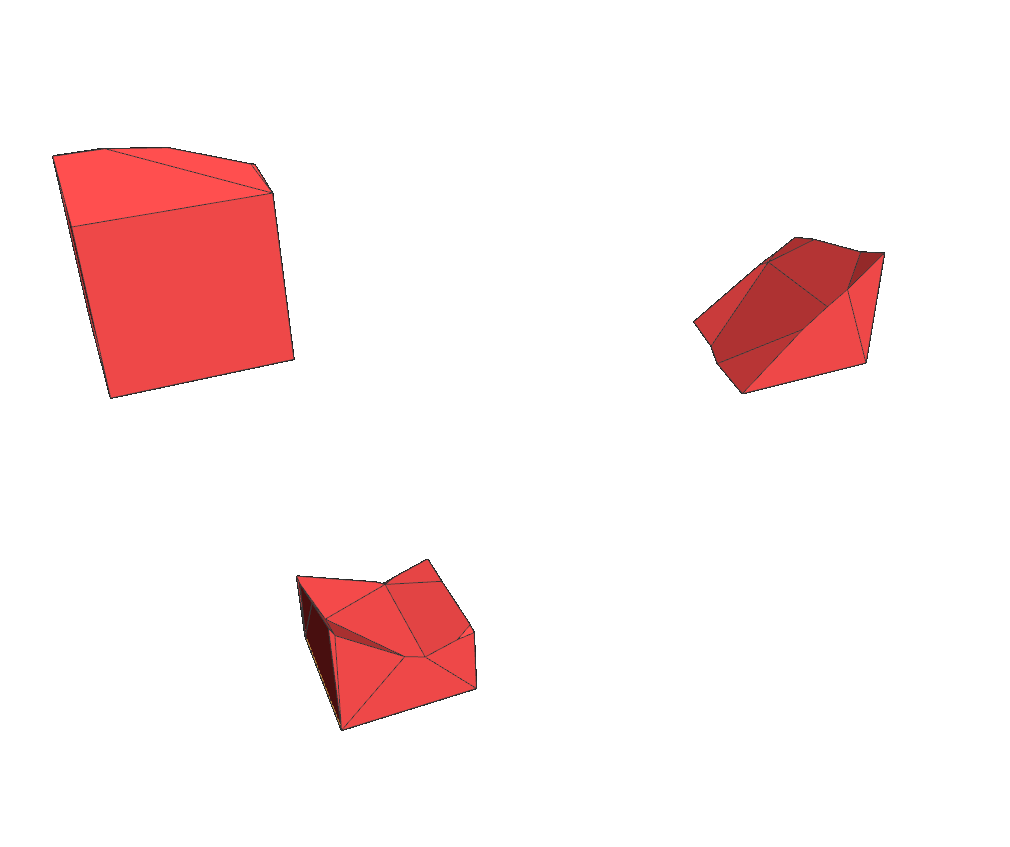
\includegraphics[scale=0.125]{media/3-celeris/zoom/zoom1.png}
\label{fig:zoom1}}		
\hfill
\subfigure[]{%
		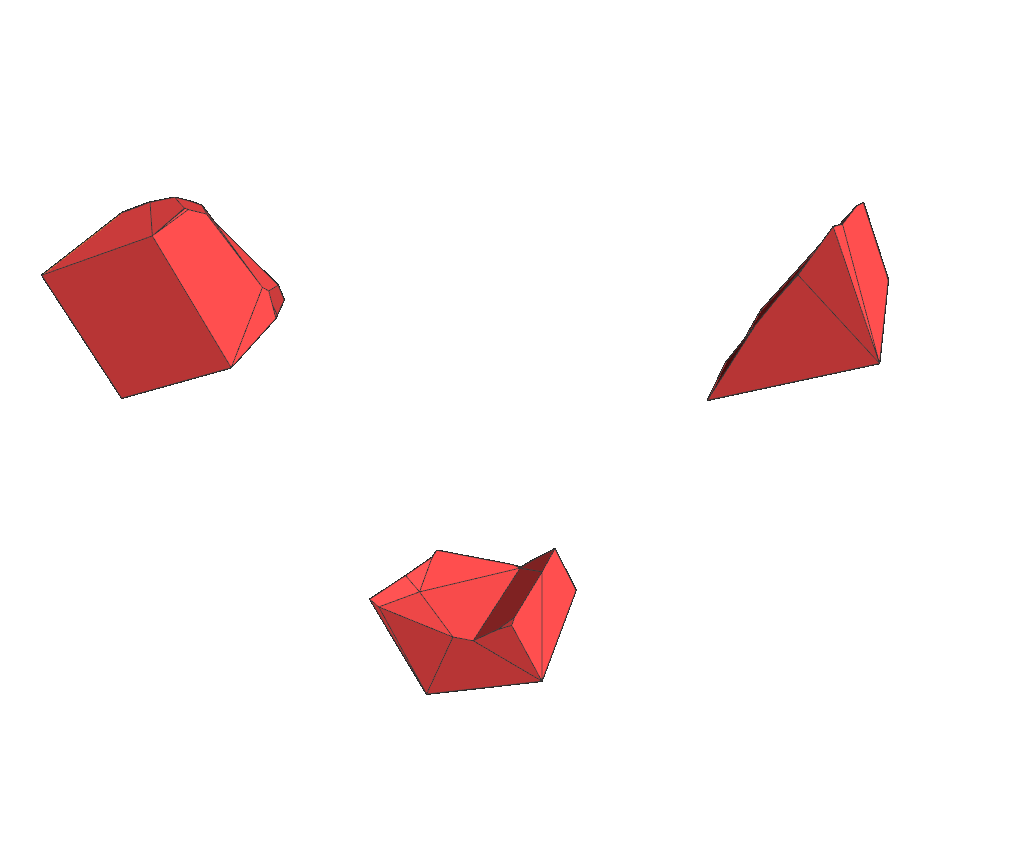
\includegraphics[scale=0.125]{media/3-celeris/zoom/zoom2.png}
\label{fig:zoom2}}		
\hfill
\subfigure[]{%
		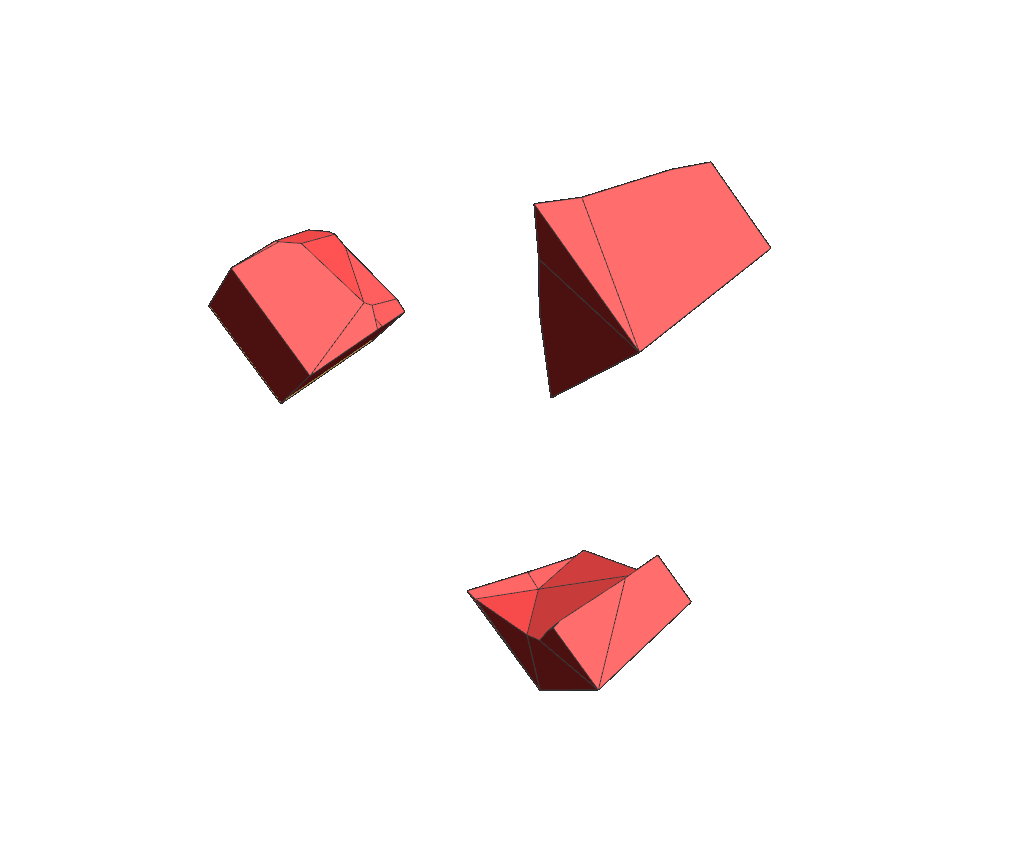
\includegraphics[scale=0.125]{media/3-celeris/zoom/zoom3.png}
\label{fig:zoom3}}		
\subfigure[]{%
		\includegraphics[scale=0.125]{media/3-celeris/zoom/zoom4.png}
\label{fig:zoom4}}	
\hfill
\subfigure[]{%
		\includegraphics[scale=0.125]{media/3-celeris/zoom/zoom5.png}
\label{fig:zoom5}}		
\hfill
\subfigure[]{%
		\includegraphics[scale=0.125]{media/3-celeris/zoom/zoom6.png}
\label{fig:zoom6}}	
\caption{Three example arbitrary polyhedral elements presented at different angles}
\label{fig:zoom}
\end{figure}

As it pertains to image-based modeling and simulation, the greatest benefit that polyhedral approaches offer is a separation between the \textit{simulation resolution} and the \textit{geometric resolution}. More detail will come in \chapref{4} regarding the polyhedral element formulation, but for this discussion the key is that nodal degrees of freedom are only defined at the points involving the background mesh, independent of the input b-rep. Thus, one can simultaneously retain a high-fidelity description of a surface while performing a simulation at a significantly lower resolution. For the other meshing approaches described in this chapter, the volume mesh resolution is implicitly constrained by the input surface mesh resolution. For complex geometries found in biological tissues, the surface mesh resolution is almost always sacrificed to avoid an unwieldy number of degrees of freedom in the subsequent finite element solution.

For the same bi-ventricular surface mesh of the \textit{ex vivo} human heart example generated by the algorithm described in the previous section, volume meshes are compared between linear polyhedral elements and quadratic tetrahedral elements. Linear polyhedral elements are chosen for comparison because they behave and perform like linear hexahedra, and thus are sufficient for generating accurate solutions. The same surface mesh with desired resolution of 50k points and desired maximum element volume of 2 $mm^3$ is supplied to: the sculpt routine in Celeris; the Delaunay tetrahedralization routine in Tetgen; and the advancing front routine in Simpleware. ~\figref{compdof} shows that for this example, the polyhedral approach reduces the system size by a factor of 2 or more. The reduction in system size stems first from the fact that the polyhedral elements are lower order compared to the tetrahedral elements (87$\%$ of the 2.5 million DOF in the Simpleware mesh correspond to midside nodes), and second from not requiring an unnecessarily large number of surface \textit{nodes} to accommodate the large number of surface \textit{points}. It should be emphasized that even at this surface resolution, a noticeable degree of geometric features is sacrificed. The greater the importance of geometric fidelity, the greater the value the polyhedral approach offers in reducing the system size.

\begin{figure}[ht!]
\centering
		\includegraphics[scale=0.2]{media/comparison.png}
%\subfigure[]{%
%		\includegraphics[scale=0.15]{media/3-celeris/8-celeris.png}
%\label{fig:comp-1}}		
%\subfigure[]{%
%		\includegraphics[scale=0.15]{media/3-celeris/9-cardioid.png}		
%\label{fig:comp-2}}	
%\subfigure[]{%
%		\includegraphics[scale=0.15]{media/3-celeris/10-simpleware.png}
%\label{fig:comp-3}}				
%
\caption{Comparison of meshes between: linear polyhedral mesh from Celeris; quadratic tetrahedral mesh from Tetgen; and quadratic tetrahedral mesh from Simpleware. Note, Simpleware focuses on generating high-quality elements, hence the larger number of DOF compared to Tetgen.}
\label{fig:compdof}
\end{figure}

The final result of the workflow from image to image mask to b-rep to polyhedral mesh is demonstrated in ~\figref{celsuite} for \textit{ex vivo} canine and human heart ventricles from the CardioVascular Research Grid~\cite{cvgg}.

\begin{sidewaysfigure}[htbp!]
\centering
\includegraphics[width=1.0\textwidth]{media/3-celeris/7-suite.png}
\caption{Suite of polyhedral finite element meshes generated from image data \vspace{1cm}}
\label{fig:celsuite}
\end{sidewaysfigure}

%%%%%%%%%%%%%%%%%%%%%%%%%%%%%%%%%%%%%%%%%%%%%%%
%%%%%%%%%%%%%%%%%%%%%%%%%%%%%%%%%%%%%%%%%%%%%%%
\subsection{File Formats}
\label{File Formats-MESH}
File formats for volume meshes follow the same paradigm as for point clouds and surface meshes. Namely, spatial coordinates of points are listed, followed by a list of elements that are defined based on connectivities of those points. The tetrahedral meshes generated by Tetgen are stored in VTK format or \textit{Abaqus} INP~\cite{abaqus} format. Polyhedral meshes are stored in a similar manner, but each element additionally requires a listing of facet data to accommodate arbitrary polyhedral topology. For the purposes of running simulations, additional information may be included with the mesh, such as surface sets or point sets for the purposes of assigning boundary conditions.

\section{Shabaka: A Free Image-Based Meshing Tool}

The image-based meshing steps described in this chapter are assembled to form a novel image-based meshing tool \textit{Shabaka}~\cite{shab}, available on GitHub at~\href{http://github.com/omhafez/shabaka}{{\url{http://github.com/omhafez/shabaka}}}. A screenshot of the repository on GitHub is shown in~\figref{github}.

\begin{figure}[ht!]
\centering
\vspace{2.5mm}
\includegraphics[width=1.0\textwidth]{media/2-shabaka/2-surf/7-shabaka.png}
\caption{Screenshot of Github repo}
\label{fig:github}
\end{figure}

Simple instructions are available to install the code on Linux, Mac, or Windows in about 15 minutes. A bash script compiles the code and downloads library dependencies including: \textit{NRRD}~\cite{nrrd} for image mask I/O, \textit{NLopt}~\cite{nlo} for nonlinear optimization, \textit{Qhull}~\cite{barber_1996} for Voronoi partitioning, \textit{ACVD}~\cite{valette_2004} for surface decimation, and \textit{Meshlab}~\cite{meshlab} and \textit{Gmsh}~\cite{geuzaine_2009} for miscellaneous mesh tasks. Libraries are gathered from the standard APT package manager on Ubuntu and from \textit{Homebrew}~\cite{brew} on Mac. The Windows installation makes use of the \textit{Windows Subsystem for Linux (WSL)}, so installation is treated in the same manner as for Ubuntu. Unit tests are available to verify a successful installation and the utility of various components of the code.

Additional free software packages are included in the build to provide an end-to-end image-based meshing pipeline. Namely, \textit{Seg3D}~\cite{Seg3D} is included for image processing and image segmentation functionality, \textit{Tetgen}~\cite{tetgen} for tetrahedral meshing, and \textit{ParaView}~\cite{paraview} for visualization. Following a full installation of the code, the user can: process and segment a medical image in Seg3D to produce an image mask; produce a high-quality surface mesh with Shabaka; produce a tetrahedral mesh using Tetgen; and visualize the resulting mesh in ParaView. Documentation on how to efficiently segment images in Seg3D has been written and included in the GitHub repo, along with essential publications related to steps in the workflow. The tool is catered toward users of simulation, 3D printing, or visualization software. No prior knowledge or understanding of image segmentation, mesh generation, or UNIX is required.

The core code for Shabaka is written in C++ and Fortran, along with Python scripts to facilitate the interaction between different portions of the code with external packages. After processing command-line inputs, the code reads the input image mask in NRRD format. The code automatically resamples segmented images that do not exhibit isotropic voxel spacing. In this manner, the point cloud generation step may assume every input image mask has equal spacing in all three directions. The point cloud generation code in C++ is easily parallelized since interfaces are approximated for each window independently of one another. The final oriented point cloud is exported in PLY format. Voronoi site locations are generated and provided to the Voronoi partitioning tool. The surface mesh is subsequently extracted, cleaned, and decimated. The final surface is exported in both PLY and STL formats.

The code has a simple UNIX environment interface that offers a number of command-line options. Options include the ability to specify a desired mesh resolution, and whether to automatically call Tetgen to produce a tetrahedral mesh from the surface generated from Shabaka. The option is also available to call the Meshlab implementation of screened Poisson surface reconstruction as an alternative to the default Voronoi-based surface reconstruction technique. Resulting surface meshes from screened Poisson surface reconstruction tend to be over-smoothed compared to those from the Voronoi-based approach. The implementation in Meshlab performs impressively fast, though, and tends to be more robust for particularly challenging surfaces, where in rare cases Voronoi approach fails to produce a valid surface.

Shabaka is currently limited to meshing binary image masks. It can mesh multiple disjoint objects in a single image but cannot currently produce meshes from multi-label masks. Each surface is watertight and manifold, and no manual correction of the mesh is required. A surface produced from Shabaka may be used as input to any software that accepts a surface mesh as input. As it pertains to the focus of this discussion, the surface mesh is inserted into a mesh generation tool, be it Tetgen for creating a quadratic tetrahedral mesh, or Celeris for creating a linear polyhedral mesh. The surface generation step typically takes less than 5 minutes for realistic input image masks using a 2.4 GHz Intel Core i7 processor with 16 GB RAM. In all, if the user has an image mask readily available, he or she can install Shabaka and generate a high-quality surface mesh and subsequent volume mesh in less than half an hour on a typical laptop.

Shabaka has been rigorously tested against a wide variety of input images. Image masks have been meshed for the heart, brain, lungs, liver, skull, pelvis, vertebra, femur, and portions of the knee joint (see \figref{showcase}).

\begin{sidewaysfigure}[htbp!]
\centering
\vspace{2.5mm}
\includegraphics[width=1.0\textwidth]{media/2-shabaka/2-surf/6-showcase.png}
\caption{Suite of example meshes generated from image data using Shabaka}
\label{fig:showcase}
\end{sidewaysfigure}

%\chapter{Physics-Based Modeling and Simulation}
\label{chap:4}
%

Numerical approximation methods may utilize an explicit geometric description of the biological tissues to model a wide array of physical phenomena. For these purposes, the discussion will be restricted to modeling quasistatic finite-deformation nonlinear solid mechanics behavior via finite element methods. Selected relevant topics in nonlinear solid mechanics and conventional finite element methods are presented. Concepts are drawn heavily from Rashid~\cite{rashid_2017, rashid_289, rashid_212, rashid_201}, Sukumar~\cite{suku_212}, and Dafalias~\cite{dafalias_205}. Lastly, a brief summary is given of a polyhedral finite element method that is to be explored as an alternative approach in biomechanical modeling.

%%%%%%%%%%%%%%%%%%%%%%%%%%%%%%%%%%%%%%%%%%%%%%%
\section{Nonlinear Solid Mechanics}
\label{Nonlinear Solid Mechanics}

Pertinent topics of nonlinear solid mechanics will be briefly summarized herein. Biological tissues can easily experience strains of 30$\%$ or more, so finite deformation kinematics of material bodies is essential. Although dynamics are of critical importance for many biomechanical studies, the formulation will be restricted here to problems in which inertial terms are considered negligible. This assumption will suffice for the cardiac mechanics applications to be discussed in \chapref{5}, since the motion of the heart is typically taken to be quasistatic.

%%%%%%%%%%%%%%%%%%%%%%%%%%%%%%%%%%%%%%%%%%%%%%%
\subsection{Kinematical Preliminaries}

The specification of \textit{nonlinear} solid mechanics is due to \textit{geometric nonlinearities} and/or \textit{material nonlinearities}. Contact considerations may also produce nonlinearities, but will not be considered here. Geometric nonlinearities arise due to the assumed \textit{finite} deformations that occur for a body of interest $\mathcal{B}$. Unlike small deformation solid mechanics, in the case of finite deformations the fixed \textit{reference configuration} $\kappa_0$ and \textit{current configuration} $\kappa_t$ are considered distinct. The reference configuration is typically chosen as the unloaded state of the body, defined at time $t=0$. Material points in the reference configuration are defined by the position vector $\bm{X}$, and locations in the current configuration by $\bm{x}(\bm{X},t)$. The displacement $\bm{u}(\bm{X},t)$ at a material point is $\bm{u}(\bm{X},t) = \bm{x}(\bm{X},t) - \bm{X}$.

The fundamental kinematic quantity in nonlinear solid mechanics is the \textit{deformation gradient} $\bm{F} = \frac{\partial \bm{x}}{\partial \bm{X}}$, which maps infinitesimal line segments in the reference configuration $\bm{dX}$ to infinitesimal line segments in the current configuration $\bm{dx}$, namely: $\bm{dx} = \bm{F}\bm{dX}$. Given the reference configuration and deformation gradient, the current configuration of the deformed body is fully defined. The local volume change at a particular point in $\mathcal{B}$ is defined by the determinant of $\bm{F}$, known as the \textit{Jacobian}: $J = \det{\bm{F}}$.

The mapping from reference configuration to current configuration $\bm{F}$ may be decomposed into a  stretch followed by a pure rotation, or vice versa, in what is known as a \textit{polar decomposition}:
\begin{equation}
\bm{F} = \bm{R}\bm{U} = \bm{V}\bm{R}
\end{equation}
where $\bm{U}$ and $\bm{V}$ are symmetric positive definite tensors, and $\bm{R}$ is a proper orthogonal tensor. Several strain measures may be defined in terms of the deformation gradient. Refer to Chadwick~\cite{chadwick_1999} for a discussion of those definitions.

Although we will focus on quasistatic problems, numerical solutions are still obtained incrementally, and thus rate quantities derived from $\bm{F}$ also come in use. The \textit{rate of deformation} (or stretch rate) tensor $\bm{D}$ and \textit{vorticity} tensor $\bm{W}$ are defined as the symmetric and antisymmetric parts of the spatial \textit{velocity gradient} $\bm{L} = \frac{\partial \bm{v}}{\partial \bm{x}} = \dot{\bm{F}}{\bm{F}}^{-1}$. Thus, $\bm{D} = \frac{1}{2}(\bm{L} + \bm{L}^T)$, $\bm{W} = \frac{1}{2}(\bm{L} - \bm{L}^T)$, and $\bm{L} = \bm{D} + \bm{W}$.

These kinematic quantities will be heavily utilized in developing the governing equations of nonlinear solid mechanics, developing kinematic update strategies to update the solution from one time step to the next, and defining material models and boundary conditions. A more detailed account of continuum kinematics can be found in Dafalias~\cite{dafalias_205} and Chadwick~\cite{chadwick_1999}.

%%%%%%%%%%%%%%%%%%%%%%%%%%%%%%%%%%%%%%%%%%%%%%%
\subsection{Traction and Stress Measures}

We define the \textit{Cauchy traction} $\bm{t}$ at a particular location on a surface in the following manner:
\begin{equation}
\bm{t} = \lim_{\substack{{da} \rightarrow 0, \\ {\bm{n} \text{\ fixed}}}} \frac{{\bm{df}}}{da}
\end{equation}
where $\bm{da} = \bm{n}da$ is an infinitesimal unit of area in the current configuration, and $\bm{n}$ is the corresponding normal to that current-configuration surface. The term $\bm{df}$ is an infinitesimal contact force in the current configuration acting on $\bm{da}$. Thus, the Cauchy traction is defined as the \textit{current configuration force} per \textit{current configuration area} at a given point, acting on a given surface. Applying a balance of linear momentum on an infinitesimal tetrahedral body yields the following relationship: $\bm{t} = \bm{T}^T\bm{n}$. The quantity $\bm{T}$ is the \textit{Cauchy stress} tensor, which defines the current configuration force per current configuration area at a particular location in space \textit{for any surface orientation}. It is the most common measure of stress. The Cauchy stress tensor is symmetric due to conservation of angular momentum for arbitrary portions of a body of interest, and so the more commonly used relationship between Cauchy traction and Cauchy stress is $\bm{t} = \bm{T}\bm{n}$.

Other common measures of stress are the \textit{first Piola-Kirchhoff stress} $\bm{P}$ and \textit{second Piola-Kirchhoff stress} $\bm{S}$. The first P-K stress relates forces in the \textit{current configuration} to areas in the \textit{reference configuration}, and is not symmetric. The second P-K stress relates forces that have been \textit{pulled back} to the reference configuration via pre-multiplication by $\bm{F}^{-1}$ to areas in the \textit{reference configuration}.

If we define the surface normal in the reference configuration as $\bm{N}$, we may define the \textit{Piola traction} as $\bm{p} = \bm{P}\bm{N}$ in an analogous manner as was done for Cauchy stress. Cauchy and Piola tractions act in the same direction since they are both defined in terms of current configuration forces. They are related based on static equivalency of forces: $\bm{p}dA = \bm{t}da$, and thus $\bm{p} = \alpha\bm{t}$, where $\alpha = \frac{da}{dA} = J\left(\bm{N} \bm{\cdot} \bm{F}^{-1}\bm{F}^{-T}\bm{N}\right)^{1/2}$ is the \textit{area stretch}.

The Cauchy stress, first P-K stress, and second P-K stress are related to one another in the following manner:
\begin{equation}
\bm{P} = J\bm{T}\bm{F}^{-T} = \bm{F}\bm{S}
\end{equation}
These relationships arise from utilizing the area ratio and deformation gradient to transform the differential force and differential area between reference and current configurations as needed based on the desired stress measure.

%%%%%%%%%%%%%%%%%%%%%%%%%%%%%%%%%%%%%%%%%%%%%%%
\subsection{Governing Equations}
Balance of linear momentum for the body $\mathcal{B}$ in the \textit{reference configuration} amounts to the following relationship:
\begin{equation}
\int_{\partial \kappa_0}{p_i}dA + \int_{\kappa_0}\rho_0{b}_idV = 0
\end{equation}
where $\partial \kappa_0$ is the boundary of the body $\mathcal{B}$ in the reference configuration, $\rho_0$ is the mass per unit reference configuration volume, $\bm{b}(\bm{X})$ is a body force (typically gravity), and inertial terms are deemed negligible. By making use of the relationship $\bm{p} = \bm{P}\bm{N}$ and the divergence and localization theorems, the final governing equations for nonlinear solid mechanics in index notation are:
\begin{gather}
P_{ij,j} + \rho_0b_i = 0, \text{\ \ } \forall \text{\ \ } \bm{X} \in \kappa_0 \label{eqn:equilibrium} \\
{u_i} = \overline{{u}}_i \text{\ \ on\ \ } \partial_u\kappa_0 \\
{p_i} = \overline{{p}}_i\text{\ \ on\ \ } \partial_t\kappa_0
\end{gather}
where $(),_j = \frac{\partial()}{\partial {{X_j}}}$ are derivatives with respect to the reference-configuration position, $\overline{{u}}_i$ are prescribed displacement boundary conditions, ${\overline{p}_i}$ are prescribed Piola tractions, $\partial_u\kappa_0 \text{\ }\bigcup\text{\ } \partial_t\kappa_0 = \partial\kappa_0$, and $\partial_u\kappa_0 \text{\ }\bigcap\text{\ } \partial_t\kappa_0 = \emptyset$. Robin boundary conditions are omitted here for clarity. Balance of linear momentum is enforced in the \textit{reference} configuration for reasons to be explained in the next section. When the field equations above for nonlinear solid mechanics are combined with the definition of the deformation gradient and with a material model, they form a well-posed elliptic boundary value problem. They constitute what is known as the \textit{strong form} of the problem statement.

%%%%%%%%%%%%%%%%%%%%%%%%%%%%%%%%%%%%%%%%%%%%%%%
%%%%%%%%%%%%%%%%%%%%%%%%%%%%%%%%%%%%%%%%%%%%%%%
\section{The Finite Element Method in Computational Solid Mechanics}
\label{The Finite Element Method in Computational Solid Mechanics}

Finite element methods are the most popular numerical methods for approximating solutions to nonlinear solid mechanics problems. Finite element approximations are based on the \textit{weak}, or \textit{variational} problem statement. The weak form of the problem statement is presented, followed by a brief discussion of Galerkin approximations to the weak form of equilibrium, of which finite element methods are a special case~\cite{rashid_2017}. Some of the major considerations for conventional FEM are discussed, including solution of the the nonlinear residual equations, mesh considerations, constitutive models, and boundary conditions.

\subsection{Weak Form and Galerkin Approximation}

The weak form of \eqnref{equilibrium} enforces equilibrium in an average integral sense, in which the equations are dotted with a \textit{test function} $\bm{w}$ and integrated over the domain of $\mathcal{B}$ in the reference configuration:
\begin{equation}
\int_{\kappa_0}{P_{ij,j}}w_idV + \int_{\kappa_0}\rho_0b_iw_idV = 0, \text{\ \ } \forall \text{\ \ } \bm{w} \in \mathcal{V}
\end{equation}
where $\mathcal{V} = \lbrace\bm{w} \text{\ }|\text{\ } \bm{w} \in H^1(\kappa_0), \text{\ }\bm{w} = 0 \text{\ \ on\ } \partial_u\kappa_0\rbrace$.

Define a \textit{trial solution space} $\mathcal{S} = \lbrace\bm{u} \text{\ }|\text{\ } \bm{u} \in H^1(\kappa_0), \text{\ }\bm{u} = \overline{\bm{u}} \text{\ \ on\ } \partial_u\kappa_0\rbrace$  to which displacements $\bm{u}$ must belong. Utilizing the divergence theorem, the weak form of equilibrium takes the following form:

Find $\bm{u}(\bm{X},t) \in \mathcal{S}$ such that
\begin{gather}
\int_{\kappa_0}P_{ij}w_{i,j}dV - \int_{\kappa_0}\rho_0b_iw_idV - \int_{\partial_t\kappa_0}\overline{p}_iw_idA = 0 \text{\ \ } \forall \text{\ \ } \bm{w} \in \mathcal{V}
\end{gather}

The weak form is solved by \textit{Galerkin approximation}, which involves approximating $\bm{u}$ and $\bm{w}$ with linear combinations of a finite set of \textit{basis functions} $\phi_a$:
\begin{gather}
\bm{u}(\bm{X},t) = \sum\limits_{a}\bm{u}_a(t)\phi_a(\bm{X}) \\
\bm{w}(\bm{X}) = \sum\limits_{a}\bm{w}_a\phi_a(\bm{X})
\end{gather}
where $\bm{u}_a$ and $\bm{w}_a$ are nodal values. The approximation is of the Galerkin variety because the basis functions used to approximate $\bm{u}$ and $\bm{w}$ are chosen to be identical. A finite discretization of the geometry of the reference configuration $\kappa_0$ provides the nodes and elements that approximate the geometry of the body, but also serves to define the basis functions. The nodes $a$ consist of those nodes in the discretization that do not lie on $\partial_u\kappa_0$. We assume from here on that the displacement boundary conditions are homogeneous, for simplicity.

The basis functions are globally continuous functions that exhibit important features in a finite element setting, namely: 1) \textit{compact support}, meaning $\phi_a$ is nonzero only on elements that contain node $a$; 2) the \textit{Kronecker delta} property, meaning $\phi_a(\bm{X}_b) = \delta_{ab}$, where $b$ is another node in the reference configuration; and 3) \textit{partition of unity}, meaning $\sum\limits_a\phi_a(\bm{X}) = 1$ throughout the body.

Utilization of the approximations to $\bm{u}$ and $\bm{w}$, and the fact that equilibrium must hold for any choice of $\bm{w}_a$ as long as $\bm{w} \in \mathcal{V}$, leads to the finite element approximation to the weak form of equilibrium, known as the \textit{residual equations}:
\begin{equation}
R_{ia} = \int_{\kappa_0}P_{ij}\phi_{a,j}dV - \int_{\kappa_0}\rho_0b_i\phi_adV - \int_{\partial_t\kappa_0} \overline{p}_i\phi_adA = 0
\label{eqn:elresid}
\end{equation}
Shape functions and integrals are all performed in the \textit{reference configuration}, making this a \textit{total Lagrangian} formulation. Performing all integrals in the reference configuration allows the basis function derivatives to be stored, rather than recomputed for each iteration of each solution step. It also simplifies derivatives of integrals over the body because the integral domain does not depend on the solution. The global residual equations are a nonlinear system of equations, solved in steps to ensure equilibrium is enforced throughout the quasistatic loading.

\subsection{Solution of the Nonlinear Residual Equations}

The solution to the global residual equations is advanced from one equilibrium state to the next as the loading is incrementally applied, until the final equilibrium state is reached for the quasistatic problem. Assuming equilibrium has been established for time $t_n$, we seek to find equilibrium for time $t_{n+1}$ through the time step $\Delta = t_{n+1} - t_{n}$. The \textit{beginning step} will refer to $t_n$ and the \textit{end step} to $t_{n+1}$. Define the position $\overline{\bm{x}} = \bm{x}(\bm{X},t_n)$, and for the forthcoming purposes we refer to ${\bm{x}}$ specifically as $\bm{x}(\bm{X},t_{n+1})$. Define ${\bm{u}}^* = \overline{\bm{x}} - \bm{X}$. In order to solve for displacements $\bm{u} = \bm{x} - \bm{X}$ at time $t_{n+1}$, the incremental displacements $\hat{\bm{u}} = \bm{x} - \overline{\bm{x}}$ are needed so that $\bm{u}$ can be updated via $\bm{u} = {\bm{u}}^* + \hat{\bm{u}}$. Thus, when seeking to update from time $t_n$ to $t_{n+1}$, we seek the incremental displacements $\hat{\bm{u}}$ such that the global residual equations are satisfied at time $t_{n+1}$, within a specified tolerance.

The most common approach to solving the nonlinear system of equations is via a \textit{Newton-Rapshon} iterative scheme. The solution of $\bm{R}_a(t_{n+1}) = \bm{0}$ is performed via successive solution of the following \textit{linearized global residual equations}:
\begin{equation}
\frac{\partial R_{ia}}{\partial \hat{u}_{jb}} \bigg|_{k+1} \delta\hat{u}_{jb} = -R_{ia}\bigg|_{k+1}
\label{eqn:newtonraphson}
\end{equation}
where:
\begin{equation}
\delta\hat{\bm{u}} = \hat{\bm{u}}\big|_{k+1} - \text{\ }\hat{\bm{u}}\big|_k
\end{equation}
and $k$ is the iteration number. When applied successfully, the procedure iterates and corrects the incremental nodal displacements until they satisfy the residual equations. Provided appropriate time steps and convergence criteria, the scheme should in practice converge to the solution ideally in only a handful of iterations.

Populating and solving the linearized residual equations requires computing the following two terms: $\frac{\partial R_{ia}}{\partial \hat{u}_{jb}} \big|_{k+1}$ and $R_{ia}\big|_{k+1}$. The nodal residuals have been defined previously in \eqnref{elresid}. For a constant reference density, and assuming the body force is not a function of displacement, the tangent stiffness is:
\begin{equation}
\frac{\partial R_{ia}}{\partial \hat{u}_{jb}} = \int_{\kappa_0}\frac{\partial P_{ik}}{\partial \hat{u}_{jb}}\phi_{a,k}dV - \int_{\partial_t\kappa_0}\frac{\partial \overline{p}_i}{\partial \hat{u}_{jb}}\phi_adA
\end{equation}
Note, because the integrals are performed in the reference configuration, the derivatives are moved past the integral signs and applied directly to the integrands. The manner in which the integrals in these terms are performed is based on the discretization of the body $\mathcal{B}$ into a discrete \textit{mesh} of finite elements. The calculation of $P_{ij}$ and $\partial{P}_{ik}/\partial{\hat{u}_{jb}}$ relies on a careful treatment of the \textit{constitutive update} and corresponding material model. The calculation of $\overline{p}_i$ and $\partial{\overline{p}_i}/\partial{\hat{u}_{jb}}$ corresponds to the choice of traction \textit{boundary conditions}. Each of these three important components to FEM are discussed next.

%%%%%%%%%%%%%%%%%%%%%%%%%%%%%%%%%%%%%%%%%%%%%%%
\subsection{Mesh Considerations}

The integrals in the linearized residual equations are performed on an element level and subsequently combined to form the global residual and tangent stiffness terms. Integrals over a single element domain $\Omega_e \subseteq \kappa_0$ have the same form as those defining $\frac{\partial R_{ia}}{\partial \hat{u}_{jb}} \big|_k$ and $R_{ia}\big|_k$, with the exception that integrals are performed over $\Omega_e$ instead of $\kappa_0$. Thus, for each element, the quantities $\frac{\partial R^e_{ia}}{\partial \hat{u}_{jb}} \big|_k$ and $R^e_{ia}\big|_k$ are of interest.

Via the spatial discretization of $\mathcal{B}$ into elements, basis functions are decomposed into element \textit{shape functions} defined on each of the neighboring elements to the node $a$ for which $\phi_a$ is defined. Those shape functions are used to compute volume and facet integrals via an \textit{isoparametric transformation} from the physical space to a \textit{parent space}, in the following manner:
\begin{equation}
\bm{X}(\bm{\xi}) = \sum\limits_{a}\bm{X}_a{N}_a(\bm{\xi})
\end{equation}
where $\bm{X}_a$ are spatial coordinates of the element nodes, $N_a$ are the shape functions, and $\bm{\xi}$ is the position vector in the parent element domain. The transformation is \textit{isoparametric} because the same shape functions are used to interpolate nodal displacements.

Thus, the element-level residual and tangent stiffness equations take the following form:
\begin{gather}
R^e_{ia} = \int_{\Omega_e}P_{ij}N_{a,j}dV - \int_{\Omega_e}\rho_0b_iN_adV - \int_{\partial_t\Omega_e} \overline{p}_iN_adA = 0 \label{eqn:elr} \\[0.7em]
\frac{\partial R^e_{ia}}{\partial \hat{u}_{jb}} = \int_{\Omega_e}\frac{\partial P_{ik}}{\partial \hat{u}_{jb}}N_{a,k}dV - \int_{\partial_t\Omega_e}\frac{\partial \overline{p}_i}{\partial \hat{u}_{jb}}N_adA \label{eqn:elt}
\end{gather}

The \textit{order} of an element corresponds to the polynomial degree of its corresponding shape functions. Refer to Hughes~\cite{hughes_2007} for a definition of the shape functions $N_a$ for linear and quadratic tetrahedral and hexahedral elements. 

Volume and facet integrals are evaluated via numerical quadrature rules on the parent element and subsequently \textit{assembled} into the linearized global residual equations. Because the shape functions $N_a$ are functions of parent space coordinates $\bm{\xi}$, integrands are computed in the parent space and the corresponding differential element is scaled to correspond to the physical reference configuration. For volume integrals, the differential volume $dv = {d\xi}{d\eta}{d\zeta}$ is scaled by the determinant of the Jacobian of the isoparametric transformation to acquire the desired $dV$ in the physical space. Namely $J_v = \det(\frac{\partial{\bm{X}}}{\partial\bm{\xi}})$ and $dV = J_vdv$. A two-dimensional analog applies for facet integrals, in which we define $da = {d\xi}{d\eta}$, $J_f = \det(\frac{\partial{\bm{X}}}{\partial\bm{\xi}})$, and $dA = J_fda$. In this case, $\bm{\xi}$ is a two-dimensional parameterization of the particular facet of interest.

Lastly, performing the volume integral of the stress-divergence term requires computing shape function gradients $N_{a,k} = \frac{\partial N_a}{\partial X_k}$ in the physical space. We may write the derivatives in terms of parent-space derivatives in the following manner:
\begin{equation}
\frac{\partial N_a}{\partial \bm{X}} = \left(\frac{\partial \bm{X}}{\partial \bm{\xi}}\right)^{\hspace{-0.3em}-T} \hspace{0.05em} \frac{\partial N_a}{\partial \bm{\xi}}
\end{equation}

For conventional FEM, the quality of the approximating solution depends critically on the ability to map spatial coordinates of an element to its parent space with high fidelity. Thus, the notion of \textit{mesh quality} is an important consideration for automated meshing tools if the resultant mesh is to be provided to a conventional FEM code. Mesh quality metrics attempt in various ways to measure the distortion of physical elements from their corresponding parent elements. Refer to the CUBIT User Documentation~\cite{cubit_2018} for an in-depth description of mesh quality metrics.

%%%%%%%%%%%%%%%%%%%%%%%%%%%%%%%%%%%%%%%%%%%%%%%
\subsection{Constitutive Update}

The constitutive update involves updating the \textit{material state} from time $t_n$ to $t_{n+1}$ at each integration point of each element in $\mathcal{B}$. Provided the motion from $\kappa_n$ to $\kappa_{n+1}$, we seek to update all \textit{state variables} based \textit{only} on their values at $t_n$, independent of choice of reference configuration. More specifically, provided incremental displacements $\hat{\bm{u}} = \bm{u} - \bm{u}^*$ from $t_n$ to $t_{n+1}$, $P_{ij}$ evaluated at $t_n$, and state variables defined at $t_n$, we seek to determine $P_{ij}$, $\partial{P_{ik}}/\partial{\hat{u}_{jb}}$, and state variables at time $t_{n+1}$. The terms $P_{ij}$ and $\partial{P_{ik}}/\partial{\hat{u}_{jb}}$ are used to compute element-level volume integrals to ultimately populate the linearized global residual equations. State variables may take many forms depending on the material model, such as \textit{plastic strain}, \textit{back stress}, or even the deformation gradient itself. In conjunction with the stress state, the state variables should fully describe the current state of the material at that particular location.

The following discussion will center around the kinematics, material update, and subsequent contribution to the linearized residual equations for \textit{hypoelastic} materials. Hypoelastic materials are typically defined as a rate form of the Cauchy stress in terms of stretch rate $\bm{D}$:
\begin{equation}
\overset{\circ}{\bm{T}} =  {\mathbfcal{C}}\bm{D}
\end{equation}
The quantity ${\mathbfcal{C}}$ is an isotropic rank-four \textit{modulus tensor}. The \textit{Jaumann rate} of stress $\overset{\circ}{\bm{T}} = \dot{\bm{T}} + \bm{T}\bm{W} - \bm{W}\bm{T}$ is known as a \textit{co-rotational} or \textit{objective} stress rate because it behaves as $\bm{Q}\overset{\circ}{\bm{T}}\bm{Q}^T$ under a superposed rigid rotation $\bm{Q}$. Among the various objective stress rates, the Jaumann rate is chosen because it respects the notion of material state, i.e., it does not depend on any reference configuration. See Rashid for a more complete discussion on material state and its relationship to objective stress rates~\cite{rashid_1991}.

In such an incremental approach, the desired input kinematic quantities are the strain increment $\bm{D}\Delta$ and rotation increment $\hat{\bm{R}}$. Rashid's incremental kinematics algorithm~\cite{rashid_1993} computes these quantities in a manner that allows accurate updates to the material state in the presence of large increments of stretch and rotation. The algorithm will be summarized herein, as it pertains to the constitutive update to hypoelastic materials. The material model is defined in terms of Cauchy stress, but the residual and tangent stiffness terms are defined in terms of the first P-K stress, so additional considerations are required to convert relevant quantities from one stress measure to the other. The following discussion will touch upon all of these details. Because material models in biological applications tend not to be defined in an incremental sense, strategies for applying this framework to \textit{hyperelastic} materials is also covered. Finally, a brief comment on treatment of material incompressibility constraints is discussed.

\subsubsection{Incremental Kinematics}

A faithful treatment of incremental kinematics depends critically on the assumed deformation history through a time step as the material state is updated from time $t_n$ to $t_{n+1}$. Rashid~\cite{rashid_1993} assumed the path is separated into two discrete motions: a pure stretching motion at constant stretch rate $\bm{D}$, followed by an instantaneous rotation $\hat{\bm{R}}$. This assumed motion proves to generate accurate stress updates in the presence of simultaneously large stretch and rotation increments, which is not the case for other popular incremental kinematics approaches~\cite{rashid_1996}. Some preliminary kinematic quantities will be defined, followed by an algorithm to compute the approximate polar decomposition of $\hat{\bm{F}}$ to acquire $\bm{D}$ and $\hat{\bm{R}}$. Finally, a description of the subsequent steps are detailed to use this assumed deformation path within the context of element contributions to residual and tangent stiffness terms for a linear hypoelastic material.

\textbf{Kinematics Quantities}

Given the incremental displacements $\hat{\bm{u}}$, we seek to compute the quantities $\bm{D}$ and $\hat{\bm{R}}$. Much in the same way we approximate $\bm{u}$ by a linear combination of shape functions $\phi_a$, we make the same approximations for $\bm{u}^*$ and $\hat{\bm{u}}$. Since we are concerned with element-level computations here, the definitions will shift from using basis functions $\phi_a$ to using shape functions $N_a$:
\begin{align}
u_i = u_{ia}N_a, \qquad u^*_i &= u^*_{ia}N_a, \qquad \hat{u}_i = \hat{u}_{ia}N_a \\
u_{i,j} = u_{ia}N_{a,j}, \qquad u^*_{i,j} &= u^*_{ia}N_{a,j}, \qquad \hat{u}_{i,j} = \hat{u}_{ia}N_{a,j}
\end{align}
Note, the nodal values are only functions of time, and not of reference configuration position. Because this is a total Lagrangian approach, the quantities $N_a$ and $N_{a,j}$ do not depend on the solution and need only be computed once for each integration point for the entire simulation.

The corresponding deformation gradients of interest are then defined as:
\begin{equation}
\bm{F} = \frac{\partial \bm{x}}{\partial \bm{X}}, \qquad \overline{\bm{F}} = \frac{\partial \overline{\bm{x}}}{\partial \bm{X}}, \qquad \hat{\bm{F}} = \frac{\partial \bm{x}}{\partial \overline{\bm{x}}}
\end{equation}
Thus, $\bm{F}$ can be decomposed as:
\begin{equation}
\bm{F} = \hat{\bm{F}}\overline{\bm{F}}
\end{equation}
It can be shown that the deformation gradients can be written in terms of the nodal displacements and shape function gradients in the following form:
\begin{align}
F_{ij} &= \delta_{ij} + \left(u^*_{ia} + \hat{u}_{ia} \right) N_{a,j} = \delta_{ij} + \left(u^*_{ia} + \hat{u}_{ia} \right) B_{ja} \\
\overline{F}_{ij} &= \delta_{ij} + u^*_{ia} N_{a,j} = \delta_{ij} + u^*_{ia} B_{ja}
\end{align}
where $B_{ja} = N_{a,j}$ are the components of the shape function gradient for node a and element $e$, evaluated at $t_{n+1}$, and $\delta_{ij}$ are the components of the Kronecker delta.

As previously mentioned, the velocity gradient is defined as $\bm{L} = \frac{\partial \bm{u}}{\partial \bm{x}} = \dot{\bm{F}}\bm{F}^{-1} = \bm{D} + \bm{W}$. In the absence of rotation, $\dot{\bm{F}}\bm{F}^{-1} = \dot{\bm{U}}\bm{U}^{-1}$ and $\bm{L} = \bm{D}$. Combining results yields $\dot{\bm{U}}\bm{U}^{-1} = \bm{D}$. Assuming a constant rate of stretch, the calculation of the rate-of-stretch tensor involves solving the following ODE:
\begin{align}
&\dot{{\bm{U}}} = {\bm{D}}{\bm{U}}, \qquad t\in (t_n, t_{n+1}) \\
&{\bm{U}}\left(t_n\right) = \bm{I}
\end{align}
Solving the ODE and imposing the desired ${\bm{U}}(t_{n+1}) = \hat{\bm{U}}$ yields $\hat{\bm{U}} = \text{exp}(\bm{D}\Delta)$. Performing a Taylor expansion about $\hat{\bm{U}} = \bm{I}$ and making use of the right Cauchy-Green deformation tensor $\hat{\bm{C}} = \hat{\bm{U}}^2$ yields the following result: 
\begin{equation}
{\bm{D}}\Delta \approx -\frac{1}{2}(\hat{\bm C}^{-1} - {\bm{I}})+ \frac{1}{4} (\hat{\bm{C}}^{-1} - {\bm{I}})^{2} - \frac{1}{6} (\hat{\bm{C}}^{-1} - {\bm{I}})^{3}
\end{equation}

The assumption that $\hat{\bm{U}}$ is near $\bm{I}$ is valid as long as the time steps are chosen so that the stretch in each time step is relatively small. Because $\hat{\bm{C}}^{-1}$ is close to identity, we define it in terms of $\bm{A} = \bm{I} - \hat{\bm{F}}^{-1} = \bm{I} - \overline{\bm{F}}\bm{F}^{-1}$ to avoid floating point precision issues. The strain increment is then computed as follows:
\begin{gather}
\hat{\bm C}^{-1} - {\bm I} = \bm{A} \bm{A}^T - \bm{A} - \bm{A}^T \\
{\bm D}\Delta = -\frac{1}{2}(\hat{\bm C}^{-1} - {\bm I})+ \frac{1}{4} (\hat{\bm C}^{-1} - {\bm I})^{2} - \frac{1}{6} (\hat{\bm C}^{-1} - {\bm I})^{3}
\end{gather}
With the strain increment now formed, what remains is the rotation increment. The calculation of the incremental rotation $\hat{\bm{R}}$ is approximated in the following manner:
\begin{equation}
\hat{R}_{ij} = \delta_{ij}\cos\theta + \frac{1 - \cos \theta}{4Q}\alpha_i\alpha_j - \frac{\sin\theta}{2\sqrt{Q}}\varepsilon_{ijk}\alpha_{k}
\end{equation}
where $\theta$ is the rotation angle, $\boldsymbol{\alpha}$ is an intermediate quantity, $\boldsymbol{\varepsilon}$ is the alternator symbol, and $Q  =\frac{1}{4}\bm{\alpha} \bm{\cdot} \bm{\alpha}$. Special care is observed when $Q$ is close to zero. Refer to Rashid~\cite{rashid_1993} for a complete description of how the rotation increment is formed. Importantly, this approximation retains proper orthogonality of $\hat{\bm{R}}$.

Thus, the stretch rate $\bm{D}$ and incremental rotation $\hat{\bm{R}}$ have been defined in an incrementally objective manner, provided the input incremental displacement $\hat{\bm{u}}$.  It should be noted that the actual polar decomposition of $\hat{\bm{F}} = \hat{\bm{R}}\hat{\bm{U}}$ may be computed at more computational cost. The additional accuracy from an exact polar decomposition may come in use for increments involving particularly large stretches and rotations, but for most practical purposes the accuracy of the algorithm via an approximated polar decomposition is sufficient~\cite{rashid_1993}.

\textbf{Element Contribution to the Linearized Global Residual Equations}

The quantities $\bm{D}$ and $\hat{\bm{R}}$ are used in conjunction with the material model to compute $P_{ij}$ in the element residual equations. This is accomplished by computing the end step \textit{unrotated} Cauchy stress $\tilde{\bm{T}}$, forward-rotating it by $\hat{\bm{R}}$ to compute $\bm{T}$, and finally converting the Cauchy stress to the first P-K stress $\bm{P}$.

For a demonstration on how to utilize the kinematics algorithm within a finite element framework, we will address the linear hypoelastic material defined by $\overset{\circ}{\bm{T}} = \bm{\mathcal{C}}\bm{D}$. Provided $\bm{D}$, we seek to integrate the stress rate in order to update the beginning step stress $\overline{\bm{T}}$. Note that the constitutive update subroutine itself is executed completely independently of $\hat{\bm{R}}$; the rotation occurs \textit{after} the update. In the absence of rotation, i.e., $\bm{W} = \bm{0}$, the Jaumann rate reduces to the time rate and the material model simplifies to $\dot{\bm{T}} = \mathbfcal{C}\bm{D}$. Provided the beginning step Cauchy stress $\overline{\bm{T}}$, the end step unrotated stress is computed via $\tilde{\bm{T}} = \overline{\bm{T}} + \mathbfcal{C}\bm{D}\Delta$. The subroutine must also provide the \textit{tangent modulus} $\partial\tilde{\bm{T}}/\partial({\bm{D}\Delta}$), which for the case of a linear hypoelastic material is simply $\mathbfcal{C}$. For the purposes of such an incremental framework, the term $\mathbfcal{C}\bm{D}\Delta$ may be viewed as an incremental stress $\hat{\bm{T}}$. The stress is then forward rotated by $\hat{\bm{R}}$:
\begin{equation}
\bm{T} = \hat{\bm{R}}\tilde{\bm{T}}\hat{\bm{R}}^T
\end{equation}
Finally, the first P-K stress is computed via $\bm{P} = J\bm{T}\bm{F}^{-T}$.

For the contribution at a particular integration point of an element to the tangent stiffness terms, the quantity $\partial{\bm{P}}/\partial{\hat{\bm{u}}}$ is desired. This term must be computed in a manner \textit{consistent} with the constitutive update algorithm to ensure desirable convergence behavior of the Newton-Raphson scheme. Namely, this term should ideally reflect the derivative of the end step stress $\bm{P}$ \textit{as it is computed} with respect to incremental displacements $\hat{\bm{u}}$, as opposed to an analytic computation insensitive to the approximations made for the kinematic input, or a numerically approximated value via finite differences.

The derivatives are performed in a lengthy but relatively straightforward manner. Using the product rule,
\begin{equation}
\frac{\partial {\bm P}}{\partial \hat{{\bm u}}} = \frac{\partial J}{\partial \hat{\bm u}}{\bm T}{\bm F}^{-T} + J\frac{\partial {\bm T}}{\partial \hat{\bm u}}{\bm F}^{-T} + J{\bm T}\frac{\partial {\bm F}}{\partial \hat{\bm u}}^{-T}
\end{equation}

Thus, the terms of interest are ${\partial J}/{\partial \hat{\bm{u}}}$, ${\partial \bm{T}}/{\partial \hat{\bm{u}}}$, and ${\partial \bm{F}^{-T}}/{\partial \hat{\bm{u}}}$. The requisite terms to compute the derivative of the first P-K tensor with respect to incremental nodal displacements follow:
\begin{gather}
\frac{\partial J}{\partial F_{kl}} = JF_{lk}^{{-1}} \\
\frac{\partial F_{ij}}{\partial \hat{u}_{ka}} = \delta_{ik}\delta_{pa}B_{jp} \\
\frac{\partial J}{\partial \hat{u}_{ka}} = JF_{pk}^{-1}B_{pa} \\
\frac{\partial F_{ij}^{-1}}{\partial F_{kl}} = - F_{ik}^{-1}F_{lj}^{-1} \\
\frac{\partial F_{ij}^{-1}}{\partial \hat{u}_{ka}} = - F_{ik}^{-1}B_{pa}F_{pj}^{-1} \\
A_{ij} = \hat{u}_{ia}B_{ka}F^{-1}_{kj} \\
\hat{{\bm C}}^{-1} = {\bm I} - {\bm A} - {\bm A}^T + {\bm A}{\bm A}^T \\
\frac{\partial A_{ij}}{\partial \hat{u}_{ka}} = \hat{F}^{-1}_{ik}B_{pa}F^{-1}_{pj} \\
\frac{\partial \hat{C}^{-1}_{ij}}{\partial \hat{A}_{kl}} = -\delta_{ik}\delta_{jl} - \delta_{jk}\delta_{il} + \delta_{ik}A_{jl} + A_{il}\delta_{jk}
\end{gather}
\begin{equation}
\begin{aligned}
\frac{\partial ({\bm D}\Delta)}{\partial {\bm A}} = &-\frac{1}{2}\frac{\partial {\hat{\bm C}^{-1}}}{\partial \bm A} + \frac{1}{4}({\hat{\bm C}}^{-1} - {\bm I})\frac{\partial \hat{\bm C}^{-1}}{\partial {\bm A}} + \frac{1}{4}\frac{\partial \hat{\bm C}^{-1}}{\partial {\bm A}}({\hat{\bm C}}^{-1} - {\bm I}) \\
&-\frac{1}{6} \frac{\partial {\hat{\bm C}^{-1}}}{\partial \bm A} (\hat{\bm C}^{-1} - {\bm I})^{2} - \frac{1}{6}  (\hat{\bm C}^{-1} - {\bm I}) \frac{\partial {\hat{\bm C}^{-1}}}{\partial \bm A} (\hat{\bm C}^{-1} - {\bm I}) \\
&- \frac{1}{6}(\hat{\bm C}^{-1} - {\bm I})^{2} \frac{\partial {\hat{\bm C}^{-1}}}{\partial \bm A} 
\end{aligned}
\end{equation}
\begin{gather}
\frac{\partial (D_{ij}\Delta)}{\partial \hat{u}_{ka}} = \frac{\partial (D_{ij}\Delta)}{\partial A_{mn}}\frac{\partial A_{mn}}{\partial \hat{u}_{ka}} \\
\frac{\partial \hat{R}_{ij}}{\partial A_{mn}} = \frac{1}{2}(-\delta_{in}\delta_{jm} + \hat{R}_{im}\hat{R}_{nj}) \\
\frac{\partial \hat{R}_{ij}}{\partial \hat{u}_{ka}} = \frac{1}{2}\left(-\hat{F}_{jk}^{-1}(F_{pi}^{-1}B_{pa}) + \hat{R}_{im}\hat{F}_{mk}^{-1}\hat{R}_{nj}(F_{pn}^{-1}B_{pa})\right) \\
\frac{\partial \tilde{\bm T}}{\partial \hat{\bm u}} = \frac{\partial \tilde{\bm T}}{\partial ({\bm D}\Delta)}\frac{\partial ({\bm D}\Delta)}{\partial \hat{\bm u}}
\end{gather}
Finally, the derivative is forward-rotated by the incremental rotation:
\begin{equation}
\frac{\partial {\bm T}}{\partial \hat{\bm u}} = \frac{\partial \hat{\bm R}}{\partial \hat{\bm u}}{\tilde {\bm T}}{\hat{\bm R}}^{T} + {\hat{\bm R}}\frac{\partial \tilde{\bm T}}{\partial \hat{\bm u}}\hat{\bm R}^T + \hat{\bm R}\tilde{\bm T}\frac{\partial \hat{\bm R}^{T}}{\partial \hat{\bm u}}
\end{equation}
Note the calculation of ${\partial \hat{R}_{ij}}/{\partial A_{mn}}$ makes use of the assumption that $\hat{\bm{U}} \approx \bm{I}$.

Thus, the end step first P-K stress and its derivative with respect to incremental nodal displacements have been computed, and via isoparametric mapping and numerical quadrature, the element level residual and tangent stiffness integrals can be populated. Those terms are then assembled into the residual equations and solved to advance the solution to the next time step.

\subsubsection{Hyperelastic Materials}

Hyperelastic material models describe nonlinear elastic behavior under finite deformations, and are commonly utilized to model the mechanical behavior of biological or rubber-like materials. A body comprised of a hyperelastic material that undergoes mechanical deformation is an example of a  \textit{conservative system}, and thus the stress may be written as a function of a \textit{strain energy potential} $W$. Indeed, hyperelastic materials are typically defined by the strain energy, rather than by a particular stress measure.

For hyperelastic materials, the strain energy $W$ is typically defined as a function of the deformation gradient $\bm{F}$ or a related kinematic quantity, from which the stress may be computed via its relationship with $W$. In the context of a constitutive update, in contrast to the hypoelastic case, the only kinematic quantity required to compute the Cauchy stress $\bm{T}$ is the end step deformation gradient $\bm{F}$. For the purposes of the linearized residual equations, rather than the tangent modulus ${\partial \tilde{\bm{T}}}/{\partial (\bm{D}\Delta)}$, the quantity ${\partial \bm{T}}/{\partial \bm{F}}$ may be computed instead. Computing the inner product of ${\partial \bm{T}}/{\partial \bm{F}}$ with $\partial \bm{F}/\partial \hat{\bm{u}}$ finally yields the desired quantity $\partial \bm{T}/\partial \hat{\bm{u}}$. In this manner, no forward rotation of the end step stress or tangent modulus is necessary.

A hyperelastic material may still be implemented within the incremental kinematics framework that has been discussed, however. This may be desirable if it is preferred that the finite element codebase treat all materials in the same way, as opposed to computing the constitutive update and contributions to the residual equations in a fundamentally different way for hyperelastic vs. hypoelastic materials. In order to accomplish this task, the deformation gradient is stored as a state variable. Care must then be taken to accurately update the deformation gradient in the constitutive update, and to subsequently forward-rotate it afterwards. The details are henceforth described for an implementation of the Mooney-Rivlin hyperelastic material model as a means of demonstration.

\textbf{Material Model Definition}

A compressible Mooney-Rivlin material is defined by the following relationship:
\begin{align}
W = C_1(\overline{I}_1 - 3) + C_2(\overline{I}_2 - 3) + D_1(J - 1)^2
\end{align}
where $W$ is the strain energy density, $C_1$ and $C_2$ are constants related to distortional response, and $D_1$ is a constant related to volumetric response. The deformation quantities are $\overline{I}_1 = J^{-2/3}I_1$ and $\overline{I}_2 = J^{-4/3}I_2$, where $I_1$ and $I_2$ are the first and second invariants of $\bm{B} = {\bm F}{\bm F}^T$. Specifically, $I_1 = \lambda_1^2 + \lambda_2^2 + \lambda_3^2$ and $I_2 = \lambda_1^2\lambda_2^2 + \lambda_2^2\lambda_3^2 + \lambda_1^2\lambda_3^2 = \frac{1}{2}[(\text{tr}{\bm B})^2 - \text{tr}({\bm B}^2)]$, where $\lambda_i$ are the eigenvalues of the deformation gradient ${\bm F}$.

The relationship between Cauchy stress ${\bm T}$ and strain energy density $W$ is as follows:
\begin{align}
{\bm T} = \frac{1}{J}\frac{\partial W}{\partial {\bm F}}{\bm F}^{T}
\end{align}
Using this relationship, one may obtain a direct expression for the Cauchy stress ${\bm T}$ in terms of the deformation gradient:
\begin{align}
{\bm T} = \frac{2}{J}\left[\frac{1}{J^{2/3}}(C_1 + \overline{I}_1{C_2}){\bm B} - \frac{1}{J^{4/3}}C_2{\bm B}^2\right] + \left[2D_1(J-1) - \frac{2}{3J}(C_1\overline{I}_1 + 2C_2\overline{I}_2)\right]{\bm I}
\end{align}
which can be written in index notation as:
\begin{align}
T_{ij} = \frac{2}{J}\left[\frac{1}{J^{2/3}}(C_1 + \overline{I}_{1}C_2)B_{ij} - \frac{1}{J^{4/3}}C_2B_{ik}B_{kj}\right] + \left[2D_1(J-1) - \frac{2}{3J}(C_1\overline{I}_{1} + 2C_2\overline{I}_{2})\right]\delta_{ij}
\end{align}
Using the relationships $\overline{I}_{1} = J^{-2/3}I_1$ and $\overline{I}_{2} = J^{-4/3}I_2$ and reorganizing, the relationship that will be used moving forward is as follows:
\begin{align}
\label{eqn:stress}
T_{ij} = 2C_1J^{-5/3}\left[B_{ij} - \frac{1}{3}I_1\delta_{ij}\right] + 2C_2J^{-7/3}\left[I_1B_{ij} - B_{im}B_{mj} - \frac{2}{3}I_2\delta_{ij}\right] + 2D_1(J-1)\delta_{ij}
\end{align}
In the limit of small strains, this reduces to a linear elastic material if the bulk modulus $K = 2D_1$ and the shear modulus $\mu = 2(C_1 + C_2)$.

\textbf{Stress Update}

Much in the same way as is done in the hypoelastic case, we define the following:
\begin{align}
\hat{\bm {U}} &= {\bm I} + {\bm D} + \frac{1}{2}{\bm D}^2 + \frac{1}{6}{\bm D}^3
\end{align}
where we have redefined ${\bm D}\leftarrow{\bm D}\Delta$ for convenience.

We now define $\tilde {\bm F}$ as the deformation gradient at time $t_{n+1}$ prior to applying the rotation increment $\hat{\bm R}$. Specifically,
\begin{align}
\tilde {\bm F} = \hat{\bm U}\overline{\bm F} \\
{\bm F} = \hat{\bm R}\tilde {\bm F}
\end{align}

When calculating stresses for the new time step, rather than feed ${\bm F}$ into the constitutive update to calculate ${\bm T}$, we feed $\bm{D}$ to calculate $\tilde{\bm{T}}$ as is done for hypoelastic materials. This requires $\overline {\bm F}$ to be stored as a state variable, which is accordingly updated at the beginning of the constitutive routine via $\tilde {\bm F} = \hat{\bm U}\overline{\bm F} $. The quantity $\tilde{\bm{F}}$ is used to compute $\tilde{\bm T}$ via \eqnref{stress}. Note that $\tilde{\bm{T}}$ is computed based only on $\tilde{\bm{F}}$, and is not computed by incrementing $\overline{\bm{T}}$ as is done for hypoelasticity. Finally, outside of the constitutive update subroutine, the end step unrotated Cauchy stress and deformation gradient are forward rotated in the following manner:
\begin{gather}
{\bm T} = \hat{\bm R}\tilde{\bm T}\hat{\bm R}^T \\
\bm{F} = \hat{\bm{R}}\tilde{\bm{F}}
\end{gather}

\textbf{Tangent Modulus}

When stepping from time $t_n$ to $t_{n+1}$, we seek the derivative $\partial{\tilde{\bm T}}/\partial {\bm D}$, where ${\bm D}$ retains its redefinition as stretch rate \textit{multiplied by the time step}. Successive use of chain rule will be used to compute $\partial \tilde{\bm{T}}/\partial{\bm{D}}$ as follows:
\begin{equation}
\frac{\partial \tilde{\bm T}}{\partial \bm D} = \frac{\partial \tilde{\bm T}}{\partial \tilde{\bm F}}\frac{\partial \tilde{\bm F}}{\partial {\hat {\bm U}}}\frac{\partial \hat{\bm U}}{\partial {\bm D}} 
\label{eq:tanmod}
\end{equation}
The following tensor derivatives will be used repeatedly in what follows:
\begin{align}
\text{if } {\bm A} \neq {\bm A}^T\text{,}\ \ \ &\frac{\partial A_{ij}}{\partial A_{kl}} = \delta_{ik}{\delta_{jl}} \\
\text{if } {\bm A} = {\bm A}^T\text{,}\ \ \ &\frac{\partial A_{ij}}{\partial A_{kl}} = \frac{1}{2}(\delta_{ik}{\delta_{jl}} + \delta_{il}{\delta_{jk}})
\end{align}
Importantly, these derivatives are not the same for symmetric and nonsymmetric tensors.

The Taylor expansion definition of $\hat{\bm U}$ from the previous section is repeated here in index notation:
\begin{align}
\hat{U}_{ij} &= \delta_{ij} + D_{ij} + \frac{1}{2}D_{im}D_{mj} + \frac{1}{6}D_{im}D_{mn}D_{nj}
\end{align}
The derivative $\partial \hat{\bm U}/{\partial {\bm D}}$ is then:
\begin{equation}
\begin{split}
\frac{\partial \hat{U}_{ij}}{\partial D_{kl}} = &\frac{1}{2}\left[\delta_{ik}\delta_{jl} + \frac{1}{2}\delta_{ik}\delta_{ml}D_{mj} + \frac{1}{2}D_{im}\delta_{mk}\delta_{jl}\  + \right.\\
&\ \left.\ \ \frac{1}{6}\delta_{ik}\delta_{ml}D_{mn}D_{nj} + \frac{1}{6}D_{im}\delta_{mk}\delta_{nl}D_{nj} + \frac{1}{6}D_{im}D_{mn}\delta_{nk}\delta_{jl}\right] + \\
&\frac{1}{2}\left[\delta_{il}\delta_{jk} + \frac{1}{2}\delta_{il}\delta_{mk}D_{mj} + \frac{1}{2}D_{im}\delta_{ml}\delta_{jk}\  + \right.\\
&\ \left.\ \ \frac{1}{6}\delta_{il}\delta_{mk}D_{mn}D_{nj} + \frac{1}{6}D_{im}\delta_{ml}\delta_{nk}D_{nj} + \frac{1}{6}D_{im}D_{mn}\delta_{nl}\delta_{jk}\right]
\end{split}
\end{equation}
Further simplifying,
\begin{align}
\frac{\partial \hat{U}_{ij}}{\partial D_{kl}} = &\frac{1}{2}\left[\delta_{ik}\delta_{jl} + \frac{1}{2}\delta_{ik}D_{lj} + \frac{1}{2}D_{ik}\delta_{jl} + \frac{1}{6}\delta_{ik}D_{ln}D_{nj} + \frac{1}{6}D_{ik}D_{lj} + \frac{1}{6}D_{im}D_{mk}\delta_{jl}\right] + \\
&\frac{1}{2}\left[\delta_{il}\delta_{jk} + \frac{1}{2}\delta_{il}D_{kj} + \frac{1}{2}D_{il}\delta_{jk} + \frac{1}{6}\delta_{il}D_{kn}D_{nj} + \frac{1}{6}D_{il}D_{kj} + \frac{1}{6}D_{im}D_{ml}\delta_{jk}\right]
\end{align}

Now, repeating the definition for $\tilde {\bm F}$ in index notation,
\begin{align}
\tilde{F}_{ij} = \hat{U}_{im}\overline{F}_{mj}
\end{align}
The derivative ${\partial \tilde{\bm F}}/{\partial \hat{\bm U}}$ is:
\begin{align}
\frac{\partial \tilde{F}_{ij}}{\partial \hat{U}_{kl}} = \frac{1}{2}\left(\delta_{ik}\delta_{ml}\overline{F}_{mj} + \delta_{il}\delta_{mk}\overline{F}_{mj}\right)
\end{align}
and simplifying:
\begin{align}
\frac{\partial \tilde{F}_{ij}}{\partial \hat{U}_{kl}} &= \frac{1}{2}\left(\delta_{ik}\overline{F}_{lj} + \delta_{il}\overline{F}_{kj}\right)
\end{align}

With $\partial \tilde{\bm F}/\partial \hat{\bm U}$ and $\partial \hat{\bm U}/\partial {\bm D}$ specified, $\partial \tilde{\bm T}/\partial \tilde {\bm F}$ remains in order to compute the tangent modulus $\partial \tilde{\bm T}/\partial {\bm D}$. We may write the derivative as follows:
\begin{align}
\frac{\partial \tilde{\bm T}}{\partial \tilde{\bm F}} &= \frac{\partial \tilde{\bm T}}{\partial J}\frac{\partial J}{\partial \tilde {\bm F}} + \frac{\partial \tilde{\bm T}}{\partial {\tilde{\bm {B}}}}\frac{\partial {\tilde{\bm {B}}}}{\partial \tilde {\bm F}}
\end{align}
where $J = \det\tilde{\bm{F}}$ and $\tilde{\bm{B}} = \tilde{\bm{F}}\tilde{\bm{F}}^T$.

The corresponding intermediate terms are then:
\begin{align}
\frac{\partial J}{\partial {\tilde{F}}_{kl}} &= {J}{\tilde{F}}^{-1}_{lk} \\
\frac{\partial \tilde{B}_{ij}}{\partial {\tilde{F}}_{kl}} &= \delta_{ik}\delta_{ml}{\tilde{F}}_{jm} + {\tilde{F}}_{im}\delta_{jk}\delta_{ml} \\
 &=  \delta_{ik}{\tilde{F}}_{jl} + {\tilde{F}}_{il}\delta_{jk}
\end{align}
The relationship for the updated Cauchy stress is repeated here:
\begin{equation}
\begin{aligned}
T_{ij} = &\ 2C_1J^{-5/3}\left[\tilde{B}_{ij} - \frac{1}{3}I_1\delta_{ij}\right] + \\ 
&\ 2C_2J^{-7/3}\left[I_1\tilde{B}_{ij} - \tilde{B}_{im}\tilde{B}_{mj} - \frac{2}{3}I_2\delta_{ij}\right] + \\
&\ 2D_1(J-1)\delta_{ij}
\end{aligned}
\end{equation}
Then,
\begin{equation}
\begin{aligned}
\frac{\partial \tilde{T}_{ij}}{\partial J} = &\frac{-10}{3}C_1J^{-8/3}\left[\tilde{B}_{ij} - \frac{1}{3}I_1\delta_{ij}\right] + \\
&\ \frac{-14}{3}C_2J^{-10/3}\left[I_1\tilde{B}_{ij} - \tilde{B}_{im}\tilde{B}_{mj} - \frac{2}{3}I_2\delta_{ij}\right] + \\ &\ 2D_1\delta_{ij}
\end{aligned}
\end{equation}

To calculate the derivative $\partial \tilde{\bm T}/\partial {\tilde{\bm {B}}}$, the following relationships are needed:
\begin{align}
\frac{\partial I_1}{\partial \tilde{B}_{kl}} &= \delta_{lk}  \\
\frac{\partial I_2}{\partial \tilde{B}_{kl}} &= I_1\delta_{kl} - \tilde{B}_{lk}
\end{align}
Finally,
\begin{equation}
\begin{aligned}
\frac{\partial \tilde{T}_{ij}}{\partial \tilde{B}_{kl}} = &\ 2C_1J^{-5/3}\left[\frac{1}{2}\left(\delta_{ik}\delta_{jl} + \delta_{il}\delta_{jk}\right) - \frac{1}{3}\delta_{ij}\delta_{kl}\right] + \\
&\ 2C_2J^{-7/3}\left[\delta_{kl}\tilde{B}_{ij} + \frac{1}{2}I_1\left(\delta_{ik}\delta_{jl} + \delta_{il}\delta_{jk}\right) -\frac{1}{2}\left(\delta_{ik}\delta_{ml} + \delta_{ik}\delta_{ml}\right)\tilde{B}_{mj} \right. + \\
&\phantom{xxxxxxxx}-\frac{1}{2}\tilde{B}_{im}\left(\delta_{mk}\delta_{jl} +\delta_{ml}\delta_{jk}\right) 
\left.- \frac{2}{3}I_1\delta_{ij}\delta_{kl} + \frac{2}{3}\delta_{ij}\tilde{B}_{lk}\right]
\end{aligned}
\end{equation}
And simplifying,
\begin{equation}
\begin{aligned}
\frac{\partial \tilde{T}_{ij}}{\partial \tilde{B}_{kl}} = &\ 2C_1J^{-5/3}\left[\frac{1}{2}\delta_{ik}\delta_{jl} + \frac{1}{2}\delta_{il}\delta_{jk} - \frac{1}{3}\delta_{ij}\delta_{kl}\right] + \\
&\ 2C_2J^{-7/3}\left[\delta_{kl}\tilde{B}_{ij} + \frac{1}{2}I_1\delta_{ik}\delta_{jl} + \frac{1}{2}I_1\delta_{il}\delta_{jk} -\frac{1}{2}\delta_{ik}\tilde{B}_{lj} -\frac{1}{2}\delta_{il}\tilde{B}_{kj} \right. + \\
&\left.\phantom{xxxxxxxx}-\frac{1}{2}\tilde{B}_{ik}\delta_{jl} -\frac{1}{2}\tilde{B}_{il}\delta_{jk} - \frac{2}{3}I_1\delta_{ij}\delta_{kl} + \frac{2}{3}\delta_{ij}\tilde{B}_{lk}\right]
\end{aligned}
\end{equation}
Thus, all terms have been defined in the calculation of the tangent modulus $\partial{\tilde{\bm{T}}}/\partial{\bm{D}}$. Like the stress and state variables, the tangent modulus is forward-rotated elsewhere in the finite element code prior to contributing to the linearized global residual equations, in the same manner described previously.

The procedure for implementing a hyperelastic material into an FEM code that only accepts hypoelastic materials has thus been established, and will be used again in \chapref{5} for implementing the mechanical behavior of cardiac tissue.

\subsubsection{Incompressibility}

Special measures must be taken to avoid \textit{volumetric locking} for materials with an incompressibility constraint. Volumetric locking occurs when there is a large mismatch between the material's apparent stiffness in deviatoric deformation compared to its volumetric deformation~\cite{rashid_2017}. The most common approach to \textit{fully} enforcing incompressibility is a \textit{mixed pressure-displacement} formulation, in which the pressure is treated as an independent variable and interpolated independently from displacement. For displacement-only formulations, however, the constraint may be enforced in a \textit{nearly incompressible} sense.

Enforcement of near-incompressibility on an integration-point level results in the displacement solution being too small, though. That is, the mesh is artificially too ``stiff.'' This volumetric locking phenomenon occurs because modes of deformation (referred to as \textit{hourglass modes} for quad or hex elements) are prevented even though they preserve the volume over the entire element.

Thus, the constraint is relaxed by enforcing incompressibility only on an element level. This amounts to modifying the incremental deformation gradient $\hat{\bm{F}}$ at each of the integration points of an element such that the dilatation is replaced by an element-averaged value, while the deviatoric deformation is unmodified. Thus, at each of the integration points, $\hat{\bm{F}}$ is replaced by $\doublehat{\bm{F}}$ in the following manner:
\begin{align}
\doublehat{\bm{F}}  &= \left(\frac{\det\bm{G}}{\hat{J}}\right)^{1/3}\hat{\bm{F}} \\
\bm{G} &= \frac{1}{|\overline{\Omega}|} \int_{\overline{\Omega}} \hat{\bm{F}}dv
\end{align}
where $\hat{J} = \det\hat{\bm{F}}$, $\overline{\Omega}$ is the element at its beginning-step configuration, and ${|\overline{\Omega}|}$ is its volume.

It should be noted that $\det\doublehat{\bm{F}}$ only approximates the overall volume change of the corresponding element. Nonetheless, the approach has been shown to approximate the exact solution under mesh refinement with sufficient accuracy for hex-8 and quad-4 elements. Refer to Rashid~\cite{rashid_2017} and Doll \textit{et al.}~\cite{doll_2000} for a more comprehensive description of volumetric locking for incompressible materials and how to address it, as well as a more detailed commentary on the F-bar method.

\subsection{Boundary Conditions}
The mechanical boundary conditions (BCs) considered here either prescribe displacements or tractions on the boundary of the body. Displacement boundary conditions on $\partial_u\kappa_0$ are enforced on the corresponding nodal displacements belonging to that surface. In the event that the prescribed displacements do not depend on the solution, the corresponding nodal values are no longer considered unknowns. Indeed, the nodes $a$ in the residual equations refer only to those nodes in $\kappa_0$ not belonging to $\partial_u\kappa_0$.

Traction boundary conditions prescribe the Piola traction $\overline{\bm{p}}$ in the residual equations over the patch of facets comprising $\partial_t\kappa_0$. The Piola traction may be directly specified, or the Piola pressure, Cauchy traction, or Cauchy pressure may be enforced. For the latter three options, the boundary condition must be converted to a Piola traction to fit into the form of the total Lagrangian residual equations. Enforcing the latter three BCs in a finite deformation setting is nontrivial. Specifically, facet contributions to the residual and stiffness terms require the area stretch $\alpha$ and current configuration normal $\bm{n}$ to be computed, along with their derivatives with respect to incremental nodal displacements.

Cauchy and Piola \textit{follower loads} may also be considered, in which case the normal and shear tractions ``follow'' the local orientation of the facet in the current configuration. Those BCs are less common and will not be discussed here, however. The remaining discussion revolves around the implementation of Piola tractions, Piola pressures, Cauchy tractions, and Cauchy pressures into a nonlinear finite element code. The task involves computing $\overline{\bm{p}}$ for the residual and ${\partial \overline{\bm{p}}}/{\partial {\hat {\bm{u}}}}$ for the tangent stiffness.

Calculations for the traction boundary conditions all stem from the formation of ${\bm {da}} = \alpha{\bm n}$ in the current configuration for the facet of interest. The quantity $\alpha{\bm n}$ is found via the cross product of orthonormal in-plane deformed material line directions in the current configuration: ${\alpha}{\bm n} = {\bm F}{\bm M}_1 \times {\bm F}{\bm M}_2$. For each integration point of a particular facet element, the four boundary conditions mentioned are then enforced based on the following calculations:

If Cauchy pressure $\overline{p}_c$ is prescribed, then $\bm {\overline{p}} = {-\overline{p}_c}\alpha{\bm n}$ and $\frac{\partial \overline{\bm{p}}}{\partial \hat {\bm{u}}} = {-\overline{p}_c}\frac{\partial (\alpha {\bm n})}{\partial {\hat {\bm{u}}}}$, where:
\begin{align}
\alpha{\bm n} &= {\bm F}{\bm M}_1 \times {\bm F}{\bm M}_2 \\
\frac{\partial (\alpha{\bm n})}{\partial {\hat {\bm{u}}}} &= (\frac{\partial {\bm F}}{\partial {\hat {\bm{u}}}}{\bm M}_1 \times {\bm F}{\bm M}_2) + ({\bm F}{\bm M}_1 \times \frac{\partial {\bm F}}{\partial {\hat {\bm{u}}}}{\bm M}_2)
\end{align}
If Cauchy traction $\overline{\bm{t}}$ is prescribed, then $\overline{\bm{p}} = \alpha{\overline{\bm{t}}}$ and $\frac{\partial \overline{\bm{p}}}{\partial {\hat {\bm{u}}}} = \frac{\partial \alpha}{\partial {\hat {\bm{u}}}}{\overline{\bm{t}}}$, where:
\begin{align}
{\alpha \bm n}, \ \frac{\partial (\alpha {\bm n})}{\partial {\hat {\bm{u}}}} &\text{ computed as before} \nonumber \\
\alpha &= [\alpha {\bm n} \bm{\cdot} \alpha {\bm n}]^{1/2} \\
 \frac{\partial{\alpha}}{\partial {\hat {\bm{u}}}} &= \frac{1}{\alpha}\frac{\partial({\alpha {\bm n}})}{\partial {\hat {\bm{u}}}} \bm{\cdot} ({\alpha \bm n})
\end{align}
If Piola pressure $\overline{p}_p$ is prescribed, then $\overline{\bm{p}} = {-\overline{p}_p}{\bm n}$ and $\frac{\partial \overline{\bm{p}}}{\partial {\hat {\bm{u}}}} = {-\overline{p}_p}\frac{\partial {\bm n}}{\partial {\hat {\bm{u}}}}$, where:
\begin{align}
{\alpha \bm n}, \ &\frac{\partial (\alpha {\bm n})}{\partial {\hat {\bm{u}}}}, \ \alpha, \ \frac{\partial \alpha}{\partial {\hat {\bm{u}}}} \text{ computed as before} \nonumber \\
{\bm n} &= \frac{1}{\alpha}(\alpha {\bm n}) \\
\frac{\partial {\bm n}}{\partial {\hat {\bm{u}}}} &= -\frac{1}{\alpha^2}(\alpha {\bm n}) + \frac{1}{\alpha}\frac{\partial (\alpha{\bm n})}{\partial {\hat {\bm{u}}}}
\end{align}

Finally, If Piola traction $\overline{\bm{p}}$ is prescribed: $\overline{\bm{p}}$ is explicitly defined and $\frac{\partial \overline{\bm{p}}}{\partial {\hat {\bm{u}}}} = {\bm 0}$.

In order to perform these steps, the deformation gradient $\bm{F}$, its derivative ${\partial \bm{F}}/{\partial \hat{\bm{u}}}$, and the local material line directions $\bm{M}_1$ and $\bm{M}_2$ in the reference configuration must be computed for each integration point of each facet element. The following intermediate quantities are required to do so: 1) shape function values $N_a$ (which are simply evaluated at the integration points), 2) the ratio $J_f$ of differential areas between reference configuration and parent space, 3) the reference configuration normal ${\bm {N}}$, and 4) the in-plane shape function gradients ${\bm {g}}_a$. The remaining discussion is centered around computing those values.

To determine these quantities, assume a parametrization $\bm{X} \in \Omega^m$ for a particular facet element $m$ is available in the reference configuration in the physical space. For conventional finite element methods, the parameterization is provided by shape functions defined in the parent space: ${X}_{i} = \sum\limits_{a}{X}_{ia}{N}_a(\xi_i)$, where parameterization variables $\xi_i$ are the parent space coordinates. The cross product of ${\partial{\bm {X}}}/{\partial \xi_1}$ and ${\partial{\bm {X}}}/{\partial \xi_2}$ defines a vector that points normal to the facet in the reference configuration, with magnitude equal to the differential area spanned by ${\partial{\bm {X}}}/{\partial \xi_1}$ and ${\partial{\bm {X}}}/{\partial \xi_2}$. This magnitude and direction are indeed the quantities $J_f$ and ${\bm {N}}$ we desire, respectively.

With $\bm{N}$ defined, the local orthonormal in-plane directions in the reference configuration $\bm{M}_1$ and $\bm{M}_2$ straightforwardly follow. Calculation of the material line segment ${\bm {M}}_1$ is performed by choosing the basis vector ${\bm {e}}_p$ that is closest to lying in the plane defined by ${\bm N}$, projecting that basis vector onto the plane defined by $\bm{N}$, and scaling it to be unit magnitude. The second direction ${\bm M}_2$ is then calculated simply via ${\bm {N}} \times {\bm {M}}_1$.

In-plane shape function gradients $\bm{g}_a$ remain to be defined, which are used to reconstruct the deformation gradient $\bm{F}$ and its derivatives within the facet integral subroutine. We seek to calculate the in-plane shape function gradients in the reference configuration $\bm{g}_a = \frac{\partial N_a}{\partial \bm{X}}$ in terms of $\bm{M}_1$ and $\bm{M}_2$. We may then define ${\bm {g}}_a = {h_{1a}}{\bm {M}}_1 + {h_{2a}}{\bm {M}}_2$, where the coefficients $h_{1a}$ and $h_{2a}$ must still be determined.

If we define ${\bm {M}}$ as the 3$\times$2 matrix whose columns are ${\bm {M}}_1$ and ${\bm M}_2$, and $\bm{h}_a$ as the 2$\times$1 column vector with components $h_{1a}$ and $h_{2a}$, we may write ${\bm g}_a = {\bm M}{\bm h}_a$. The shape function gradients with respect to the parameterization variables are then \mbox{$\frac{\partial N_a}{\bm{\partial {\xi}}} = {\bm g}_a \bm{\cdot} \frac{\partial {\bm X}}{\bm{\partial {\xi}}}$}. Using the definition for ${\bm g}_a$, this can be written as:
\begin{align}
\frac{\partial N_a}{\partial {\bm \xi}} &= {\bm g}_a \bm{\cdot} \frac{\partial {\bm X}}{\partial {\bm \xi}} \\
&= {\bm M}{\bm h}_a \bm{\cdot} \frac{\partial {\bm X}}{\partial {\bm \xi}} \\
&= (\frac{\partial {\bm X}}{\partial {\bm \xi}}^T{\bm M}){\bm h}_a \\
&= {\bm H}{\bm h}_a
\end{align}
The matrix ${\bm H} = \frac{\partial {\bm X}}{\partial {\bm \xi}}^T{\bm M}$ maps in-plane shape function gradients $h_{ia}$ acting in directions ${\bm M}_i$ into shape function gradients in directions of the parameterized variables ${\xi_j}$. The components $h_{ia}$ are then found from ${\bm h}_a = {\bm H}^{-1}\frac{\partial N_a}{\partial {\bm \xi}}$. Finally, ${\bm g}_a$ is formed using the relation ${\bm g}_a = {h_{1a}}{\bm M}_1 + {h_{2a}}{\bm M}_2$.

The previous discussion simplifies to a concise set of calculations that are performed at each integration point of a facet:
\begin{align}
\frac{\partial X_{i}}{\partial \xi_j} &= \sum_a X_{i}\frac{\partial N_a}{\partial \xi_j}, \text{\ \ \ \ }i=1,3, \text{\ \ }j = 1,2 \\
{\bm{dA}} &= \frac{\partial{\bm{X}}}{\partial \xi_1} \times \frac{\partial {\bm {X}}}{\partial \xi_2} \\
J_f &= | {\bm {dA}}| \\
{\bm N} &= \frac{1}{J_f}{\bm {dA}} \\
\text{Determine } p &\text{ such that } N_p = \min_i{|N_i|} \\
{\bm M}_1 &=\frac{ ({\bm I} - {\bm N}\otimes{\bm N}){\bm e}_p}{|({\bm I} - {\bm N}\otimes{\bm N}){\bm e}_p|} \\
{\bm M}_2 &= {\bm N} \times {\bm M}_1 \\
H_{ij} &= \frac{\partial {\bm X}}{\partial \xi_i} \bm{\cdot} {\bm M}_j, \text{\ \ \ \ }i=1,\text{2}, \text{\ \ }j = 1,\text{2} \\
{\bm h}_a &= {\bm H}^{-1} \frac{\partial N_a}{\partial {\bm \xi}} \\
{\bm g}_a &= h_{1a}{\bm M}_1 + h_{2a}{\bm M}_2
\end{align}
Finally,
\begin{align}
F_{ij} &= \delta_{ij} + \sum_a{u_{ia}g_{ja}} \\
\frac{\partial F_{ij}}{\partial \hat{u}_{kb}} &= \delta_{ik}g_{jb}
\end{align}

Thus, $\bm{F}$, ${\partial \bm{F}}/{\partial \hat{\bm{u}}}$, $\bm{M}_1$, and $\bm{M}_2$ have all been defined and can be used to compute the various boundary conditions described previously.

\subsection{Additional Topics}
Finite element methods is a rich field with many more pertinent topics related to producing accurate and efficient approximations to physical phenomena. Additional important topics, to name only a few, include: more advanced nonlinear solution schemes to the residual equations; direct and iterative solvers for large matrix computations; mesh refinement/convergence studies and \textit{a posteriori} error estimation; 
enforcement of \textit{fully} incompressible materials, for example with a mixed pressure-displacement formulation; numerical modeling of frictionless and frictional contact; numerical modeling of material separation, including fracture; numerical modeling of thin structures and additional approaches to mitigating element locking; implicit and explicit approaches to modeling the dynamics of solid bodies; and coupling of multiple physical phenomena. Refer to Hughes~\cite{hughes_2000} as a starting point for addressing some of these topics.

%%%%%%%%%%%%%%%%%%%%%%%%%%%%%%%%%%%%%%%%%%%%%%%
%%%%%%%%%%%%%%%%%%%%%%%%%%%%%%%%%%%%%%%%%%%%%%%
\section[A Polyhedral Finite Element Method in Computational Solid \\ Mechanics]{\texorpdfstring{A Polyhedral Finite Element Method in \\ Computational Solid Mechanics}{A Polyhedral Finite Element Method in Computational Solid \\ Mechanics}}
\label{A Polyhedral Finite Element Method in Computational Solid Mechanics}

As discussed in this chapter, conventional finite element methods utilize analytic shape functions that are defined in a parent space, from which a mapping is defined to compute element-level integration via numerical quadrature rules. This mapping introduces restrictions on the element geometry and topology that, for practical purposes, limit the element type to a very small set of choices. For complex geometries seen in biological tissues, the restrictions on element geometry and topology cause serious challenges for the automatic meshing algorithms discussed in \chapref{3}. \textit{Polyhedral finite element methods} attempt to improve upon conventional techniques by defining shape functions and corresponding integration rules for general  \textit{polyhedral} element topologies. Polyhedral FEM exhibits elements that do not need to conform to the topology of a fixed parent element, thus removing debilitating constraints on automatic meshing tools for the purposes of simulation. At the same time, these methods enjoy much of the same desirable properties of conventional FEM, including high quadrature efficiency and straightforward FEM-like boundary condition enforcement.

The construction of polygonal and polyhedral finite element shape functions, including for concave geometries, are discussed in detail by Sukumar \textit{et al.}~\cite{sukumar_2006} and Manzini \textit{et al.}~\cite{manzini_2014}. Rashid \textit{et al.}~\cite{rashid_2012, rashid_2015} offer a particular flavor of polyhedral FEM methods known as the \textit{Partitioned Element Method (PEM)}, whose implementation offers a robust workflow for CAD-based simulation. An important feature of PEM stems from the realization that the shape functions do not need to be defined over the entire element domain. Instead, only their values and gradients need be defined at the quadrature points of the element.

The Partitioned Element Method explicitly partitions each element into polyhedral \textit{cells}. They are constructed in a tolerance-aware sense that is robust in the presence of geometric pathologies. These subdomains are used to define a discontinuous piecewise linear shape function in the physical space over each element, along with its corresponding quadrature rule. Shape functions are constructed first on element edges, then on element faces, and finally over the three-dimensional element. The shape function construction on lower-order topes informs the construction on higher-order topes. In each case, a quadratic objective function is minimized in an attempt to minimize jumps in the shape function and its gradients along cell interfaces. The solution of this minimization problem leads to a small linear system to be solved for each element in a mesh at the beginning of the simulation. Quadrature rules are defined based on specifying the integration points at the cell centroids and the integration weights as the cell volumes. Additional constraints to the minimization problem ensure \textit{quadrature consistency} (the property that a constant stress field exactly satisfies the weak form of equilibrium on a single element). PEM has been shown to converge at the same rate as FEM~\cite{rashid_2012}. Many of the considerations outlined are nontrivial - refer to the resources cited for a more rigorous and complete accounting of the method.

As it pertains to the user of simulation software for performing biomechanical simulations, PEM offers three critical benefits related to meshing. First, the meshing procedure need not adhere to the strict geometric and topological requirements of conventional FEM, allowing for more robust automated mesh generation. Second, as discussed in \chapref{3}, the simulation and geometric resolutions are decoupled. Namely, the simulation resolution need only be refined to the extent that accurate solutions can be provided, rather than being constrained in some way by the number of points and polygons used to the describe the surface of the object. And lastly, linear PEM elements have been shown to produce accurate results, which together with the previous benefit can significantly reduce the number of DOF compared to automated higher-order FEM approaches. This reduction in DOF was demonstrated in \figref{compdof}. A further exploration of the polyhedral approach and its benefits and will be conducted alongside conventional FEM in modeling cardiac mechanics in \chapref{5}.

%%%%%%%%%%%%%%%%%%%%%%%%%%%%%%%%%%%%%%%%%%%%%%%
%\chapter{Application: Cardiac Mechanics}
\label{chap:5}
%

REFER HEAVILY TO LIVERMORE FINAL REPORT \\
%~\cite{heartmech} \\
%~\cite{newheartpaper} \\
Describe generation of segs and meshes: \\
threshold \\
level set \\
connected components \\
fill holes \\
dilate-erode \\
manual fine-tuning \\

\begin{figure}[ht]
\centering
\subfigure[]{%
		\includegraphics[scale=0.081]{media/4-cardioid/2-activationtime.png}
\label{fig:supp1}}
\subfigure[]{%
		\includegraphics[scale=0.081]{media/4-cardioid/3-fibers.png}
\label{fig:supp2}}
\subfigure[]{%
		\includegraphics[scale=0.081]{media/4-cardioid/4-tagged.png}
\label{fig:supp3}}
%
\caption{Mechanics modeling considerations: (a) muscle fiber orientations, (b) electrical activation times, and c) surface tagging and prescription of corresponding boundary conditions.}
\label{fig:supp}
\end{figure}

\begin{figure}[ht]
\centering
\subfigure[]{%
		\includegraphics[scale=0.5]{media/4-cardioid/5-pv/pressure_volume-1.pdf}
\label{fig:pv1}}		
\subfigure[]{%
		\includegraphics[scale=0.5]{media/4-cardioid/5-pv/pressure_volume-2.pdf}
\label{fig:pv2}}		
%
\caption{Results from Cardioid simulation: (a) P-V loop of left ventricle, (b) pressure time history in left and right ventricles.}
\label{fig:pv}
\end{figure}

\begin{figure}[ht!]
\centering
\subfigure[]{%
		\includegraphics[scale=0.057]{media/4-cardioid/6-vid/a.png}
\label{fig:snaps1}}		
\subfigure[]{%
		\includegraphics[scale=0.057]{media/4-cardioid/6-vid/b.png}
\label{fig:snaps2}}		
\subfigure[]{%
		\includegraphics[scale=0.057]{media/4-cardioid/6-vid/c.png}
\label{fig:snapsf3}}		
\subfigure[]{%
		\includegraphics[scale=0.057]{media/4-cardioid/6-vid/d.png}
\label{fig:snaps4}}		
%
\caption{Deformed mesh from Cardioid simulation at different stages of cardiac cycle. Panels (a), (b), (c), and (d) correspond to the stages in the P-V loop denoted in FIGREF ???.}
\label{fig:snaps}
\end{figure}

\begin{figure}[ht]
\centering
\subfigure[]{%
		\includegraphics[scale=0.18]{media/5-verif/1-gurev2/gurev2.png}
\label{fig:beams1}}		
\subfigure[]{%
		\includegraphics[scale=0.18]{media/5-verif/2-gurev3/gurev3.png}
\label{fig:beams2}}		
\subfigure[]{%
		\includegraphics[scale=0.18]{media/5-verif/3-gurev4/gurev4.png}
\label{fig:beams3}}		
\subfigure[]{%
		\includegraphics[scale=0.18]{media/5-verif/4-land1/land1.png}
\label{fig:beams4}}		
%
\caption{Undeformed (bottom) and deformed (top) configurations for cantilever beam verification problems: (a) Gurev P2: bending, (b) Gurev P3: torsion, c) Gurev P4: active contraction, and (d) Land P1: bending. The red curve denotes the curve over which displacements and positions are recorded for comparison of results.}
\label{fig:beams}
\end{figure}

\begin{figure}[ht]
\centering
\subfigure[]{%
		\includegraphics[scale=0.18]{media/5-verif/5-land2/land2-1.png}
\label{fig:ventricles1}}		
\subfigure[]{%
		\includegraphics[scale=0.18]{media/5-verif/5-land2/land2-2.png}
\label{fig:ventricles2}}		
\subfigure[]{%
		\includegraphics[scale=0.18]{media/5-verif/6-land3/land3-1.png}
\label{fig:ventricles3}}		
\subfigure[]{%
		\includegraphics[scale=0.16]{media/5-verif/6-land3/land3-2.png}
\label{fig:ventricles4}}		
%
\caption{Undeformed (left) and deformed (right) configurations for single ventricle verification problems: (a,b) Land P2: inflation, and (c,d) Land P3: inflation and active contraction. The red curve denotes the curve over which displacements and positions are recorded for comparison of results.}
\label{fig:ventricles}
\end{figure}

\begin{figure}[ht]
\centering
\subfigure[]{%
		\includegraphics[scale=0.48]{media/5-verif/1-gurev2/gurev2-1.pdf}
\label{fig:gurev2-1}}		
\subfigure[]{%
		\includegraphics[scale=0.48]{media/5-verif/1-gurev2/gurev2-2.pdf}
\label{fig:gurev2-2}}		
%
\caption{Results for Gurev P2 verification problem: (a) Displacement magnitude along diagonal axis, with (b) details for the free end of the beam}
\label{fig:gurev2}
\end{figure}

\begin{figure}[ht!]
\centering
\subfigure[]{%
		\includegraphics[scale=0.48]{media/5-verif/2-gurev3/gurev3-1.pdf}
\label{fig:gurev3-1}}		
\subfigure[]{%
		\includegraphics[scale=0.48]{media/5-verif/2-gurev3/gurev3-2.pdf}
\label{fig:gure3-2}}		
%
\caption{Results for Gurev P3 verification problem: (a) Displacement magnitude along diagonal axis, with (b) details for the fixed end of the beam. The results for imitor and Celeris are indistinguishable in these plots.}
\label{fig:gurev3}
\end{figure}

\begin{figure}[ht!]
\centering
\subfigure[]{%
		\includegraphics[scale=0.48]{media/5-verif/3-gurev4/gurev4-1.pdf}
\label{fig:gurev4-1}}		
\subfigure[]{%
		\includegraphics[scale=0.48]{media/5-verif/3-gurev4/gurev4-2.pdf}
\label{fig:gurev4-2}}		
%
\caption{Results for Gurev P4 verification problem: (a) Displacement magnitude along diagonal axis, with (b) details for the free end of the beam. The results for imitor and Celeris are indistinguishable in these plots.}
\label{fig:gurev4}
\end{figure}

\begin{figure}[ht!]
\centering
\subfigure[]{%
		\includegraphics[scale=0.48]{media/5-verif/4-land1/land1-1.pdf}
\label{fig:land1-1}}		
\subfigure[]{%
		\includegraphics[scale=0.48]{media/5-verif/4-land1/land1-2.pdf}
\label{fig:land1-2}}	
\subfigure[]{%
		\includegraphics[scale=0.48]{media/5-verif/4-land1/land1-3.pdf}
\label{fig:land1-3}}			
%
\caption{Results for Land P1 verification problem: (a) Deformed position of midline, with (b) details for the free end of the beam. Panel (c) shows the deformed position of the point $\mathbf{X} = (10, 0.5, 1)$ for each of the simulation codes.}
\label{fig:land1}
\end{figure}


\begin{figure}[ht!]
\centering
\subfigure[]{%
		\includegraphics[scale=0.48]{media/5-verif/5-land2/land2-1.pdf}
\label{fig:land2-1}}		
\subfigure[]{%
		\includegraphics[scale=0.48]{media/5-verif/5-land2/land2-2.pdf}
\label{fig:land2-2}}	
\subfigure[]{%
		\includegraphics[scale=0.48]{media/5-verif/5-land2/land2-3.pdf}
\label{fig:land2-3}}			
%
\caption{Results for Land P2 verification problem: (a) Deformed position of middle of the ventricle wall, with (b) details at the inflection point (top right) and the apical region (bottom right). Panel (c) shows the deformed position of the apex at the endo- and epicardium for each of the simulation codes.}
\label{fig:land2}
\end{figure}

\begin{figure}[ht!]
\centering
\subfigure[]{%
		\includegraphics[scale=0.48]{media/5-verif/6-land3/land3-1.pdf}
\label{fig:land3-1}}		
\subfigure[]{%
		\includegraphics[scale=0.48]{media/5-verif/6-land3/land3-2.pdf}
\label{fig:land3-2}}	
%
\caption{Results for Land P3 verification problem: (a) Deformed position of middle of the ventricle wall, with (b) details at the inflection point (top right) and the apical region (bottom right).}
\label{fig:land3}
\end{figure}

\begin{figure}[ht!]
\centering
\subfigure[]{%
		\includegraphics[scale=0.48]{media/5-verif/6-land3/land3-3.pdf}
\label{fig:land3.2-1}}		
\subfigure[]{%
		\includegraphics[scale=0.48]{media/5-verif/6-land3/land3-4.pdf}		
\label{fig:land3.2-2}}	
\subfigure[]{%
		\includegraphics[scale=0.48]{media/5-verif/6-land3/land3-5.pdf}
\label{fig:land3.2-3}}			
	
%
\caption{Results for Land P3 verification problem: (a) The same deformed position of middle of the ventricle wall, shown in the $x-y$ plane, with (b) details at the inflection point. Panel (c) shows the deformed position of the apex at the endo- and epicardium for each of the simulation codes.}
\label{fig:land3.2}
\end{figure}

{http://www.springer.com/us/book/9781441907295} \\
Cardioid science on saturday Youtube
$heart_papers$
papers Mark mentions in SOW

%%%%%%%%%%%%%%%%%%%%%%%%%%%%%%%%%%%%%%%%%%%%%%%
%%%%%%%%%%%%%%%%%%%%%%%%%%%%%%%%%%%%%%%%%%%%%%%
\section{Problem Description}
\label{Problem Description}

%%%%%%%%%%%%%%%%%%%%%%%%%%%%%%%%%%%%%%%%%%%%%%%
%%%%%%%%%%%%%%%%%%%%%%%%%%%%%%%%%%%%%%%%%%%%%%%
\section{Material Model}
\label{Material Model}

\subsection{Passive Stress}
\label{Passive Stress}

\subsection{Active Stress}
\label{Active Stress}

%%%%%%%%%%%%%%%%%%%%%%%%%%%%%%%%%%%%%%%%%%%%%%%
%%%%%%%%%%%%%%%%%%%%%%%%%%%%%%%%%%%%%%%%%%%%%%%
\section{Fiber Generation}
\label{Fiber Generation}

%%%%%%%%%%%%%%%%%%%%%%%%%%%%%%%%%%%%%%%%%%%%%%%
%%%%%%%%%%%%%%%%%%%%%%%%%%%%%%%%%%%%%%%%%%%%%%%
\section{Boundary Conditions}
\label{Boundary Conditions}

%%%%%%%%%%%%%%%%%%%%%%%%%%%%%%%%%%%%%%%%%%%%%%%
%%%%%%%%%%%%%%%%%%%%%%%%%%%%%%%%%%%%%%%%%%%%%%%
\section{Solver}
\label{Solver}

%%%%%%%%%%%%%%%%%%%%%%%%%%%%%%%%%%%%%%%%%%%%%%%
%%%%%%%%%%%%%%%%%%%%%%%%%%%%%%%%%%%%%%%%%%%%%%%
\section{Simulation Results}
\label{Simulation Results}


%\chapter{Future Work}
\label{chap:6}

Potential for future work exists in a number of directions, both in the near term and long term. More pressing research opportunities and improvements to the tools discussed are outlined, followed by a discussion of grander directions in which the field of image-based modeling and simulation is moving.

%%%%%%%%%%%%%%%%%%%%%%
%%%%%%%%%%%%%%%%%%%%%%
\section{Short Term}
\label{Short Term}

Tasks related to completing the full demonstration of polyhedral FEM in Celeris, improving the image-based meshing tool Shabaka, and improving the cardiac mechanics code Cardioid are described herein.

\subsection[A Polyhedral Finite Element Demonstration in Cardiac \\ Mechanics]{\texorpdfstring{A Polyhedral Finite Element Demonstration in Cardiac Mechanics}{A Polyhedral Finite Element Demonstration in Cardiac Mechanics}}
\label{A Polyhedral Finite Element Demonstration in Cardiac Mechanics}

Pending some minor fixes in the Celeris codebase, the first task would be to complete the verification problems outlined in \chapref{5}. Given the accurate results provided by Imitor, it is expected that Celeris will produce satisfactory results as well, at least for cuboidal PEM elements. The benefit of polyhedral FEM for these purposes is again three-fold: complex geometries may be meshed automatically, the mesh resolution is not constrained directly by the surface resolution, and linear element shape functions avoid an unnecessary increase in DOF. The single ventricle geometry is quite simple, though, and thus automated hex and tet meshing that is not particularly constrained by the surface resolution is possible in this case. Nonetheless, the completion of the verification problems will at a minimum show the capability to automatically generate a general polyhedral mesh and run accurate solutions while avoiding quadratic elements.

Once the implementation has been fully verified, the next step would be to run a complete bi-ventricular cardiac mechanics simulation using polyhedral finite elements. The highest priority is first to demonstrate capability, followed by a more direct comparison of results and computational effort between the quadratic tet mesh in Cardioid and the polyhedral mesh in Celeris. This would require a convergence study in both codes to ensure that the coarsest possible meshes were being used while still attaining accurate results. This likely would also include a more comprehensive comparison of results, for example by measuring and comparing stresses and strains at particular locations of interest. As of yet, there is no definitive answer to whether polyhedral FEM is a viable replacement for quadratic tetrahedra in cardiac mechanics simulations, but the preliminary results look very promising. A direct demonstration of polyhedral FEM's desirable features would be quite useful.

It is worth mentioning that for polyhedral FEM to have competitive runtimes, the associated code would likely need to incorporate an iterative solver and potentially be restructured to run on a distributed memory system. There is nothing unique to polyhedral FEM that would prohibit those changes though. Depending on the degree to which the number of DOF can be reduced, and the desired simulation resolution, a direct solver on a shared memory system may well be more than sufficient, but that would need to be proven. Additionally, the notion of \textit{element quality} has not yet been well defined in the context of polyhedral elements. Concepts related to mapping shape functions from the physical space to a parent space are obviously not an issue, but it is still unclear the degree to which elements near the boundary may be ``ill-shaped'' before solution accuracy begins to degrade. A complete bi-ventricular simulation would certainly clarify some of these matters.

Ultimately, polyhedral finite element methods would exhibit its advantages most strongly in image-based biomechanics for geometries that require a high resolution to define the surface, and for problems that require frequent remeshing during the simulation. It is hoped that these next steps would further solidify the promise of such an approach.

\subsection{Improvements to Image-Based Meshing Code}
\label{Improvements to Image-Based Meshing Code}

A vast number of improvements may be made to the image-based meshing code Shabaka, which would open several additional application areas for which the code could be useful.

The highest yield improvements involve expanding the capabilities of the interface approximation and surface reconstruction tasks. Interface approximation would be significantly improved if expanded to handle regions of high curvature or even sharp edges and corners. This would involve creating more interface ``templates'' in addition to the plane approximation that is currently in place. The most favorable additions would include a paraboloid interface, an edge interface, and a corner interface. For these interfaces, several point/normals may be placed for a single window. This extension would significantly improve the accuracy (and resulting density) of points in regions of high curvature, and even allow image-based mesh generation for objects with sharp edges and corners. The ability to generate high quality surfaces involving sharp features would usher opportunities for more conventional mechanical and aerospace engineering applications.

Another important extension to Shabaka is handling multi-material image masks. As of now, the algorithm is restricted to binary image masks. Although plenty of work is still performed for single object meshes, the state of the art tools available for image-based meshing tend to have capability for multiple materials. Ideas may be gleaned from Dyadechko and Shashkov~\cite{dyadechko_2008}, who reconstruct polygonal multi-material interfaces for simulations of incompressible fluid flows. Although currently only developed for two dimensions, their work provides a partitioning scheme for multiple material junctions based on similar notions of minimizing error in the moments of volume. Once the matter is sorted, Shabaka may link with the same mesh generation tools as before, which are already well-equipped to handle multi-material b-reps. This improvement would significantly expand the range of biomedical applications, most notably to the brain and the knee (see \figref{polyknee}).

\begin{sidewaysfigure}[htbp!]
\centering
		\includegraphics[width=1.0\textwidth]{media/7-polyknee/fullmesh.png}
%
\caption{Polyhedral mesh of human knee generated from Open Knee b-rep~\cite{erdemir_2015}}
\label{fig:polyknee}
\end{sidewaysfigure}

Improving the surface reconstruction of an oriented point cloud is also critical. Work is underway within the Celeris codebase to allow for a \textit{tolerance-aware} Voronoi partioning scheme~\cite{rashid_2019}, with similar philosophy and implementation to how polyhedral meshes are constructed from b-reps. This could potentially mitigate the issue of ``cross-talk'' facets discussed in \chapref{3}. If a tolerance-aware approach does not resolve the issues caused by the current Voronoi approach, the surface reconstruction task may be better suited to follow the approach outlined by Meyer \textit{et al.}~\cite{meyer_2008}. Provided an oriented point cloud, they perform a Delaunay tetrahedralization on the point cloud itself, and then extract the surface of interest based on \textit{Delaunay} facets that share different material types.

A less urgent task would involve improving the interaction between image, image mask, and surface mesh. Work may be explored to generate point clouds directly from medical images, bypassing the image segmentation step altogether. Considering the complexity of image segmentation techniques, avoiding that intermediate step would likely prove to be a difficult task. A more fruitful intermediate term approach may be to extract more information from the image mask. For example, the underlying image carries a range of intensity values near the interface approximated by the image mask. Retaining that information with the segmented image can lead to more accurate surfaces. Indeed, Young \textit{et al.}~\cite{young_2008}, for example, make use of ``soft segmentations'', or what they call the \textit{partial volume effect} to produce smoother surfaces. In essence, they honor the fact that the image and image mask are inextricably linked.

From a software utility standpoint, the Shabaka code may be improved in some tangible ways as well. The bash build script should be replaced by a \textit{CMake}~\cite{cmake} file for a more robust installation process in downloading and installing external packages. In the same vein, the Windows version ideally would not depend on the Windows Subsystem for Linux, which is essentially a temporary workaround due to familiarity with accessing third-party software in a UNIX environment. In the interest of a faster and more reliable build, more tools should be developed within Shabaka to avoid dependence on admittedly fragile third-party software.

Finally, a necessary step in proving the quality of results from Shabaka is a numerical validation of point clouds and surface meshes for a variety of example inputs. Error measures should be defined and calculated to quantify the degree to which the interface approximations generate point clouds that honor the original surfaces from a medical image. Similarly, the quality of resulting surface meshes should be measured numerically, perhaps again comparing moments of volume between the original image mask and the resulting surface. Of course, these error measures ideally should be compared to other popular surface reconstruction and image-bashed meshing algorithms. Lastly, as coined by Young \textit{et al.}~\cite{young_2008}, the notion of \textit{convergence to geometry} must be further explored and understood. Specifically, mesh convergence from CAD data typically assumes there is no error in the geometric accuracy of the solid model itself. In image-based meshing, however, a finite number of sampling points are used to reconstruct the b-rep, and thus there is inevitably an error associated with that approximation. Shabaka currently allows the user to specify the number of points to define the surface of interest, but developing guidelines for how many points are actually required to ``converge to geometry'' would be quite informative and useful.

\subsection{Improvements to Cardiac Mechanics Code}
\label{Improvements to Cardiac Mechanics Code}

The cardiac mechanics code Cardioid has room for improvement on several fronts now that a robust workflow for cardiac simulations has been established. Arguably the most interesting tasks from a computing standpoint are moving towards a complete coupling between the mechanics, electrophysiology, and \textit{hemodynamics} (i.e., circulatory model) codes. As mentioned before, only a one-way coupling currently exists between the electrophysiology and mechanics codes. In reality, of course, the large deformations experienced in the heart certainly affect the manner in which electrical waves propagate within the body. Likewise, the pressures in each ventricle are certainly not spatially uniform. The current lumped circulatory model could be replaced by a complete fluid dynamics code modeling blood flow, such as the one developed by Gounley \textit{et al.}~\cite{gounley_2017}, which is also affiliated with Lawrence Livermore National Laboratory. In this case, the volume constraints would be replaced by fluid-structure interaction considerations.

Other important improvements include the treatment of boundary conditions at the base and epicardium of the heart. As of now, the less-than-convincing BCs that displacements at the base be restricted in-plane, and that an arbitrary strip of the epicardium is restrained in all three directions, must be improved. A simple improvement to the epicardium BCs, for example, could involve modeling the heart inside a fixed elastic medium. \textit{In vivo} behavior of the heart should certainly guide those decisions. Although not urgent, providing the ability to generate muscle fiber orientations directly from DTMRI data would also improve the Cardioid code. Although the process has not been perfected, some groups have been successful in moving away from model-based fiber generation~\cite{yang_2012, zhukov_2003}.

Even without the improvements suggested here, several studies may now be performed with the current model. Validation of results must be the highest priority as Cardioid moves toward answering clinical questions. Additionally, given a working model, a whole range of sensitivity studies may be performed to determine what meshing and modeling parameters are most influential. Some questions include:
\begin{itemize}[noitemsep]
\item How sensitive are the results to approximating the surface of the heart accurately? Is diligently capturing the inner structures in the ventricles necessary? Some preliminary work hints that papillary muscles, for example, do not play a significant role~\cite{korte_2019}.
\item How does the accuracy of fiber orientation affect the solution? Do fibers generated from a rule-based approach produce different results compared to those generated from DTMRI data?
\item How do different passive and active constitutive models affect the solution?
\item How does mesh quality affect the iterative solver performance?
\item To what degree do the boundary conditions influence the solution?
\item How important is it to include electromechanics coupling and/or fluid-structure interaction?
\end{itemize} 
Lastly, much in the same way convergence to geometry should be guaranteed by Shabaka, a mesh convergence study should be performed to determine the desired resolution of cardiac meshes for converged simulation results.

%%%%%%%%%%%%%%%%%%%%%%
%%%%%%%%%%%%%%%%%%%%%%
\section{Long Term}
\label{Long Term}

A brief discussion here covers the future of image-based modeling and simulation and how it might interact more with machine learning and 3D printing in the coming years.

\subsection{Simulation of Clinical Trials}
\label{Simulation of Clinical Trials}

Although plenty of opportunities still exist to improve the tools involved in image-based modeling and simulation, the problem of robustly performing patient-specific modeling has more or less been solved. Patient-specific treatments and medical devices are already a reality. The important next step in the field is to combine simulations related to a single patient with statistical and/or machine learning technologies for large populations of patients. One may refer to this extension as \textit{simulation of clinical trials}. To properly perform such an ambitious task will involve several important considerations moving forward. Among the most important are: appropriate assignment of material properties for each patient, appropriate boundary conditions for each patient, performing rigorous verification, validation, and potentially even uncertainty quantification (VVUQ) ~\cite{NAP13395}, and heavily relying on high performance computing to perform large numbers of simulations in a timely manner.

For example, the project ``A Machine Learning System to Guide Clinical Procedures in Real-Time'' currently funded by Lawrence Livermore National Laboratory will utilize the image-based modeling workflow that has been described, and will certainly need to attend to many of the considerations mentioned. That project aims to improve surgical treatment of \textit{ventricular fibrillation}, the deadliest form of cardiac arrhythmia. The research aims to produce a large virtual patient dataset based on imaging data, from which machine learning tools can determine optimal locations to \textit{ablate} (or remove) portions of an arrhythmic heart. The proposed virtual population of 10-40k patients will be based on a real patient population of roughly 100. The focus of this document has been to robustly generate quality meshes for accurate simulation. With that task at a working level, the focus will shift to ensuring accurate depictions of the material behavior, boundary conditions, and overall validation of results. Provided those tasks are accomplished, machine learning-guided simulations can improve real surgeries and save real lives.

\subsection[Applications in Rapid Prototyping and Additive Manufacturing]{\texorpdfstring{Applications in Rapid Prototyping and Additive \newline Manufacturing}{Applications in Rapid Prototyping and Additive \newline Manufacturing}}
\label{Applications in Rapid Prototyping and Additive Manufacturing}

Rapid prototyping and additive manufacturing have begun to revolutionize many facets of engineering, and biomechanics applications are no exception. Indeed, in 2017 the FDA issued a guideline titled ``Technical Considerations for Additive Manufactured Medical Devices''~\cite{fda3_2016}, signifying the degree to which the technology is beginning to play an important role in medical device design.

The input requirements for a 3D printer are in fact identical to those of a CAD-based mesh generation tool: a closed, manifold surface mesh is required in both cases. STL files are by far the most popular surface mesh file format for 3D printing. Some of the STL surfaces generated using Shabaka were printed with a \textit{fused deposition modeling (FDM)} printer, in which melted material is extruded layer by layer to produce a three-dimensional object (see~\figref{3dprint}). A visual print of an object can be quite illuminating, even for a surgeon or technician who has already become accustomed to 3D computer models.

\begin{sidewaysfigure}[htbp!]
\centering
		\includegraphics[width=1.0\textwidth]{media/6-3dprint/3dprint.jpg}
%
\caption{Suite of 3D-printed organs using surface meshes generated from novel image-based meshing tool Shabaka}
\label{fig:3dprint}
\end{sidewaysfigure}

Of the many challenges to robustly create 3D-printed objects using fused deposition modeling, some include:
\begin{itemize}[noitemsep]
\item reliability, i.e., getting the same output for multiple instances of the same input;
\item optimizing the many print design parameters, including extruder temperature, layer thickness, support structure, and extruder outflow rate;
\item determining the desired print precision; and
\item cost
\end{itemize}
It was deemed that fused deposition modeling is better suited for simple prototyping applications, and not for precise or large-scale applications. Other (more expensive) printing technologies will likely be more appropriate for production-level prints, such as \textit{stereolithography (SLA)}, in which a laser cures liquid resin into hardened plastic via \textit{photopolymerization}, or \textit{selective laser sintering (SLS)}, in which a high-powered laser fuses small particles of polymer or metal powder~\cite{3dprints}.

Tack \textit{et al.}~\cite{tack_2016} outlined a comprehensive review of 3D printing in medical settings. They covered various surgical domains in which 3D-printed surgical guides and implants have impacted the field, including orthopedics, cerebrovascular, cardiovascular, and dental applications. Clearly 3D printing enjoys several directions in which it could potentially improve the field of biomedical engineering, and its intimacy with simulation will certainly increase over time.

%\chapter{Conclusions}
\label{chap:7}
%

This work presented a new image-based modeling and simulation pipeline. The workflow includes a novel algorithm for generating b-reps from binary image masks. The algorithm first generates a dense oriented point cloud approximating the surface of the object by minimizing a relative error functional measuring the difference in geometric properties between the voxelated image mask and the approximated surface. The point cloud generation step is highly parallelizable since the calculation of each point is independent of one another. A Voronoi-based surface reconstruction algorithm was presented, that inserts Voronoi sites based on the point cloud, computes a Voronoi partition, and extracts the surface based on material assignments of the Voronoi sites. The surface generation algorithm performs well for surfaces that do not exhibit regions of excessively high curvature or sharp features. The surface is subsequently cleaned and decimated to produce a watertight, manifold surface mesh that may be used as input to CAD-based meshing software, 3D printers, or visualization programs. The code was linked with third-party image segmentation and CAD-based meshing software, and packaged into a free, open-source tool named Shabaka, available on Linux, Mac, or Windows. The tool installs in a matter of 15 minutes, and meshes are generated from image masks typically in less than 5 minutes on a personal computer. Dozens of example meshes were created to demonstrate capability.

The surface mesh of a human heart was generated using the tools described, and used as input to produce quadratic tetrahedral and polyhedral bi-ventricular meshes for the purposes of finite element analysis. Cardiac mechanics simulations were performed on massively parallel systems to model the mechanical behavior of a beating human heart using quadratic tets within the code Cardioid. In the process, existing tools to model muscle fiber orientations, simulate the electrophysiology, and assign boundary conditions were streamlined for expedient results. The fiber orientations, boundary condition tags, activation times, and pressure boundary conditions were imported into the polyhedral code Celeris for the purposes of running the same simulation using polyhedral FEM. Polyhedral finite elements offer the promise of a robust and automated image-based modeling and simulation workflow while potentially significantly reducing the system size compared to conventional FEM approaches. That reduction is most importantly achieved because the simulation mesh resolution is completely independent of the geometric resolution. The material model involved in producing the cardiac simulations was implemented in the polyhedral code and verified against a suite of test problems. Additional steps will complete the verification of the polyhedral implementation, demonstrate capability of polyhedral FEM in cardiac mechanics, and showcase the ability to produce accurate results with fewer degrees of freedom.The work has shown promising preliminary results in demonstrating PFEM as an alternative to conventional approaches in modeling cardiac mechanics.

The image-based modeling and simulation workflow is to be used in a project that performs cardiac simulations in conjunction with machine learning techniques to improve procedures treating cardiac arrhythmia. Provided that the role of patent-specific material parameters are patient-specific boundary conditions are better understood, and models begin to incorporate more rigorous validation and uncertainty quantification techniques, \textit{in silico} modeling has the potential to significantly impact how medicine is performed. Simulation of clinical trials, optimization of surgical techniques and medical device designs, and additive manufacturing, are among the most compelling and impactful areas that may benefit from this technology.

\bibliography{references}

% The UMI abstract uses square brackets!
\UMIabstract[The abstract that is submitted to UMI must be formatted as shown in the example here. The body of the abstract cannot exceed 350 words. It should be in typewritten form, double-spaced, and on bond paper. It is important to write an abstract that gives a clear description of the content and major divisions of the dissertation]

\end{document} 